\chapter{General topology}
\section{Topological structures}
\subsection{Topological spaces}
\begin{definition}
A \textbf{topological structure} (or, more briefly, a \textbf{topology}) on a set $X$ is a structure given by a set $\mathcal{T}$ of subsets of $X$, having the following properties:
\begin{itemize}
\item[(O1)] $\emp,X\in\mathcal{T}$.
\item[(O2)] Every union of sets of $\mathcal{T}$ is a set of $\mathcal{T}$.
\item[(O3)] Every finite intersection of sets of $\mathcal{T}$ is a set of $\mathcal{T}$.
\end{itemize}
The sets of $\mathcal{T}$ are called \textbf{open sets} of the topological structure defined by $\mathcal{T}$ on $X$.
\end{definition}
A \textbf{topological space} is a set endowed with a topological structure. The elements of a topological space are often called points. When a topology has been defined on a set $X$, this set is said to be the set undering the topological space $X$.
\begin{example}
If $X$ is any set, the collection of all subsets of $X$ is a topology on $X$; it is called the \textbf{discrete topology}. The collection consisting of $X$ and $\emp$ only is also a topology on $X$; we shall call it the \textbf{indiscrete topology}, or the \textbf{trivial topology}.
\end{example}
\begin{example}
Let $X$ be a set; let $\mathcal{T}_{fc}$ be the collection of all subsets $U$ of $X$ such that $U^c$ either is finite or is all of $X$. Then $\mathcal{T}_{fc}$ is a topology on $X$, called the \textbf{finite complement topology}. Both $X$ and $\emp$ are in $\mathcal{T}_{fc}$, since $X^c$ is finite and $\emp^c$ is all of $X$. If $\{U_\alpha\}$ is an indexed family of nonempty elements of $\mathcal{T}_{fc}$, to show that $\bigcap_\alpha U_\alpha$ is in $\mathcal{T}_{fc}$, we compute
\[\Big(\bigcup_\alpha U_\alpha\Big)^c=\bigcap_\alpha U_\alpha^c.\]
The latter set is finite because each set $U_\alpha^c$ is finite. If $U_1,\dots,U_n$ are nonempty elements of $\mathcal{T}_{fc}$, to show that $\bigcap_{i=1}^{n}U_i$ is in $\mathcal{T}_{fc}$, we compute that
\[\Big(\bigcap_{i=1}^{n}U_\alpha\Big)^c=\bigcup_{i=1}^{n}U_\alpha^c.\]
The latter set is a finite union of finite sets and, therefore, finite.\par
Similarly, let $\mathcal{T}_{cc}$ be the collection of all subsets $U$ of $X$ such that $U^c$ either is countable or is all of $X$. Then $\mathcal{T}_{cc}$ is a topology on $X$, called the \textbf{countable complement topology} on $X$.
\end{example}
\begin{definition}
Suppose that $\mathcal{T}_1$ and $\mathcal{T}_2$ are two topologies on a given set $X$. If $\mathcal{T}_1\sups\mathcal{T}_2$, we say that $\mathcal{T}_1$ is \textbf{finer} than $\mathcal{T}_2$; if $\mathcal{T}_1$ properly contains $\mathcal{T}_2$, we say that $\mathcal{T}_1$ is \textbf{strictly finer} than $\mathcal{T}_2$. We also say that $\mathcal{T}_2$ is \textbf{coarser} than $\mathcal{T}_1$, or \textbf{strictly coarser}, in these two respective situations. We say $\mathcal{T}_1$ is \textbf{comparable} with $\mathcal{T}_2$ if either $\mathcal{T}_1\sub\mathcal{T}_2$ or $\mathcal{T}_2\sub\mathcal{T}_1$.
\end{definition}
\subsection{Base of topologies}
For each of the examples in the preceding part, we were able to specify the topology by describing the entire collection $\mathcal{T}$ of open sets. Usually this is too difficult. In most cases, one specifies instead a smaller collection of subsets of $X$ and defines the topology in terms of that.
\begin{definition}
If $X$ is a set, a base for a topology on $X$ is a collection $\mathcal{B}$ of subsets of $X$ (called \textbf{base elements}) such that
\begin{itemize}
\item[(B1)] For each $x\in X$, there is at least one base element $B$ containing $x$.
\item[(B2)] If $x$ belongs to the intersection of two base elements $B_1$ and $B_2$, then there is a base element $B_3$ containing $x$ such that $B_3\sub B_1\cap B_2$.
\end{itemize}
\end{definition}
If $\mathcal{B}$ satisfies these two conditions, then we define the topology $\mathcal{T}$ generated by $\mathcal{B}$ as follows: A subset $U$ of $X$ is said to be open in $X$ (that is, to be an element of $\mathcal{T}$) if for each $x\in U$, there is a base element $B\in\mathcal{B}$ such that $x\in B$ and $B\sub U$. Note that each base element is itself an element of $\mathcal{T}$. We now check that the collection $\mathcal{T}$ is indeed a topology on $X$. 
\begin{proposition}
The collection $\mathcal{T}$ induced by a base $\mathcal{B}$ is a topology on $X$.
\end{proposition}
\begin{proof}
If $U$ is the empty set, it satisfies the defining condition of openness vacuously. Likewise, $X$ is in $\mathcal{T}$, since for each $x\in X$ there is some base element $B$ containing $x$ and contained in $X$. Now let us take an indexed family $(U_\alpha)_{\alpha\in A}$, of elements of $\mathcal{T}$ and consider $U=\bigcup_{\alpha}U_\alpha$. Given $x\in U$, there is an index $\alpha$ such that $x\in U_\alpha$. Since $U_\alpha$ is open, there is a base element $B$ such that $x\in B\sub U_\alpha$. Then $x\in B\sub U$, so that $U$ is open, by definition.\par
Now let us take two elements $U_1$ and $U_2$ of $\mathcal{T}$ and show that $U_1\cap U_2$ belongs to $\mathcal{T}$. Given $x\in U_1\cap U_2$, choose a base element $B_1$ containing $x$ such that $B_1\sub U_1$; choose also a base element $B_2$ containing $x$ such that $B_2\sub U_2$. The second condition for a base enables us to choose a base element $B_3$ containing $x$ such that $B_3\sub B_1\cap B_2$. Then $x\in B_3$ and $B_3\sub U_1\cap U_2$, so $U_1\cap U_2$ belongs to $\mathcal{T}$, by definition.
\end{proof}
\begin{example}
Let $\mathcal{B}$ be the collection of all circular regions (interiors of circles) in the plane. Then $\mathcal{B}$ satisfies both conditions for a base. In the topology generated by $\mathcal{B}$, a subset $U$ of the plane is open if every $x$ in $U$ lies in some circular region contained in $U$.
\end{example}
\begin{example}
Let $\mathcal{B}$ be the collection of all rectangular regions (interiors of rectangles) in the plane, where the rectangles have sides parallel to the coordinate axes. Then $\mathcal{B}$ satisfies both conditions for a base. In this case, the condition (B2) is trivial, because the intersection of any two base elements is itself a base element (or empty). As we shall see later, the base $\mathcal{B}$ generates the same topology on the plane as the base given in the preceding example.
\end{example}
\begin{example}
If $X$ is any set, the collection of all one-point subsets of $X$ is a base for the discrete topology on $X$.
\end{example}
Another way of describing the topology generated by a base is given in the following lemma:
\begin{lemma}\label{topological space open set is union of base}
Let $X$ be a set; let $\mathcal{B}$ be a base for a topology $\mathcal{T}$ on $X$. Then $\mathcal{T}$ equals the collection of all unions of elements of $\mathcal{B}$.
\end{lemma}
\begin{proof}
Given a collection of elements of $\mathcal{B}$, they are also elements of $\mathcal{T}$. Because $\mathcal{T}$ is a topology, their union is in $\mathcal{T}$. Conversely, given $U\in\mathcal{T}$, choose for each $x\in U$ an element $B_x$ of $\mathcal{B}$ such that $x\in B_x\sub U$. Then $U=\bigcup_{x\in U}B_x$, so $U$ equals a union of elements of $\mathcal{B}$.
\end{proof}
This lemma states that every open set $U$ in $X$ can be expressed as a union of base elements. This expression for $U$ is not, however, unique. Thus the use of the term "base" in topology differs drastically from its use in linear algebra, where the equation expressing a given vector as a linear combination of base vectors is unique. We have described in two different ways how to go from a base to the topology it generates.  Sometimes we need to go in the reverse direction, from a topology to a base generating it. Here is one way of obtaining a base for a given topology; we shall use it frequently.
\begin{proposition}\label{topological space base if}
Let $X$ be a topological space. Suppose that $\mathcal{B}$ is a collection of open sets of $X$ such that for each open set $U$ of $X$ and each $x$ in $U$, there is an element $B$ of $\mathcal{B}$ such that $x\in B\sub U$. Then $\mathcal{B}$ is a base for the topology of $X$.
\end{proposition}
\begin{proof}
We must show that $\mathcal{B}$ is a base. The first condition for a base is easy: Given $x\in X$, since $X$ is itself an open set, there is by hypothesis an element $B$ of $\mathcal{B}$ such that $x\in B\sub X$. To check the second condition, let $x$ belong to $B_1\cap B_2$, where $B_1$ and $B_2$ are elements of $\mathcal{B}$. Since $B_1$ and $B_2$ are open, so is $B_1\cap B_2$. Therefore, there exists by hypothesis an element $B_3$ in $\mathcal{B}$ such that $x\in B_3\sub B_1\cap B_2$.\par
Let $\mathcal{T}$ be the collection of open sets of $X$; we must show that the topology $\mathcal{T}$ generated by $\mathcal{B}$ equals the topology $\mathcal{T}$. First, note that if $U$ belongs to $\mathcal{T}$ and if $x\in U$, then there is by hypothesis an element $B$ of $\mathcal{B}$ such that $x\in B\sub U$. It follows that $U$ belongs to the topology $\mathcal{T}'$, by definition. Conversely, if $W$ belongs to the topology $\mathcal{T}'$, then $W$ equals a union of elements of $\mathcal{B}$, by the preceding lemma. Since each element of $B$ belongs to $\mathcal{T}$ and $\mathcal{T}$ is a topology, $W$ also belongs to $\mathcal{T}$.
\end{proof}
When topologies are given by bases, it is useful to have a criterion in terms of the bases for determining whether one topology is finer than another. One such criterion is the following:
\begin{proposition}
Let $\mathcal{B}_1$ and $\mathcal{B}_2$ be bases for the topologies $\mathcal{T}$ and $\mathcal{T}_2$, respectively, on $X$. Then the following are equivalent:
\begin{itemize}
\item[(\rmnum{1})] $\mathcal{T}_1$ is finer than $\mathcal{T}_2$.
\item[(\rmnum{2})] For each $x\in X$ and each base element $B_2\in\mathcal{B}_2$ containing $x$, there is a base element $B_1\in\mathcal{B}_1$ such that $x\in B_1\sub B_2$.
\end{itemize}
\end{proposition}
\begin{proof}
Assume (\rmnum{2}). Given an element $U$ of $\mathcal{T}_2$, we wish to show that $U\in\mathcal{T}_1$. Let $x\in U$. Since $\mathcal{B}_2$ generates $\mathcal{T}_2$, there is an element $B_2\in\mathcal{B}_2$ such that $x\in B_2\sub U$. Condition (\rmnum{2}) tells us there exists an element $B_1\in\mathcal{B}_1$ such that $x\in B_1\sub B_2$. Then $x\in B_1\sub U$, so $U\in\mathcal{T}_1$, by definition.\par
Conversely, assume (\rmnum{1}). We are given $x\in X$ and $B_2\in\mathcal{B}_2$, with $x\in B_2$. Now $\mathcal{B}_2$ belongs to $\mathcal{T}_2$ by definition and $\mathcal{T}_2\sub\mathcal{T}_1$ by condition (\rmnum{1}); therefore, $B\in\mathcal{T}_1$. Since $\mathcal{T}_1$ is generated by $\mathcal{B}_1$, there is an element $B_1\in\mathcal{B}_1$ such that $x\in B_1\sub B_2$.
\end{proof}
We now define three topologies on the real line $\R$, all of which are of interest.
\begin{example}
If $\mathcal{B}$ is the collection of all open intervals in the real line,
\[(a,b)=\{x\in\R:a<x<b\}\]
the topology generated by $\mathcal{B}$ is called the standard topology on the real line. Whenever we consider $\R$, we shall suppose it is given this topology unless we specifically state otherwise. If $\mathcal{B}'$ is the collection of all half-open intervals of the form
\[[a,b)=\{x\in\R:a\leq x<b\},\]
where $a<b$, the topology generated by $\mathcal{B}'$ is called the lower limit topology on $\R$. When $\R$ is given the lower limit topology, we denote it by $\R_l$. Finally let $K$ denote the set of all numbers of the form $1/n$, for $n\in\Z_+$, and let $\mathcal{B}_K$ be the collection of all open intervals $(a,b)$, along with all sets of the form $(a,b)\setminus K$. The topology generated by $\mathcal{B}_K$ will be called the $K$-topology on $\R$. When $\R$ is given this topology, we denote it by $\R_K$.
\end{example}
It is easy to see that all three of these collections are bases; in each case, the intersection of two base elements is either another base element or is empty. The relation between these topologies is the following:
\begin{proposition}
The topologies of $\R_l$ and $\R_K$ are strictly finer than the standard topology on $\R$, but are not comparable with one another.
\end{proposition}
\begin{proof}
Let $\mathcal{T}$, $\mathcal{T}_l$, and $\mathcal{T}_K$ be the topologies of $\R$, $\R_l$, and $\R_K$, respectively. Given a base element $(a,b)$ for $\mathcal{T}$ and a point $x$ of $(a,b)$, the base element $[x,b)$ for $\mathcal{T}_l$ contains $x$ and lies in $(a,b)$. On the other hand, given the base element $[x,d)$ for $\mathcal{T}_l$, there is no open interval $(a,b)$ that contains $x$ and lies in $[x,d)$. Thus $\mathcal{T}_l$ is strictly finer than $\mathcal{T}$.\par
A similar argument applies to $\R_K$. Given a base element $(a,b)$ for $\mathcal{T}$ and a point $x$ of $(a,b)$, this same interval is a base element for $\mathcal{T}_K$ that contains $x$. On the other hand, given the base element $B=(-1,1)\setminus K$ for $\mathcal{T}_K$ and the point $0$ of $B$, there is no open interval that contains $0$ and lies in $B$.\par
Finally, given the base element $[x,d)$ for $\mathcal{T}_l$, there is no base element of $\mathcal{T}_K$ that contains $x$ and lies in $[x,d)$, so $\mathcal{T}_K$ is not finer than $\mathcal{T}_l$. Conversely, given the base element $B=(-1,1)\setminus K$ for $\mathcal{T}_K$ and the point $0$ of $B$, there is no interval $[a,b)$ that contains $0$ and lies in $B$. Thus $\mathcal{T}_l$ is not finer than $\mathcal{T}_K$.
\end{proof}
\begin{example}
Let $X$ be a totally ordered set; assume $X$ has more than one element. Let $\mathcal{B}$ be the collection of all sets of the following types:
\begin{itemize}
\item[(a)] All open intervals $(a,b)$ in $X$.
\item[(b)] All intervals of the form $[a_0,b)$, where $a_0$ is the smallest element (if any) of $X$.
\item[(c)] All intervals of the form $(a,b_0]$, where $b_0$ is the largest element (if any) of $X$.
\end{itemize}
The collection $\mathcal{B}$ is a base for a topology on $X$, which is called the \textbf{order topology}.
\end{example}
A question may occur to us at this point. Since the topology generated by a base $\mathcal{B}$ may be described as the collection of arbitrary unions of elements of $\mathcal{B}$, what happens if we start with a given collection of sets and take finite intersections of them as well as arbitrary unions? This question leads to the notion of a subbase for a topology.
\begin{definition}
A \textbf{subbase} $\mathcal{S}$ for a topology on $X$ is a collection of subsets of $X$ whose union equals $X$. The topology generated by the subbase $\mathcal{S}$ is defined to be the collection $\mathcal{T}$ of all unions of finite intersections of elements of $\mathcal{S}$.
\end{definition}
We must of course check that $\mathcal{T}$ is a topology. For this purpose it will suffice to show that the collection $\mathcal{B}$ of all finite intersections of elements of $\mathcal{S}$ is a base. Given $x\in X$, it belongs to an element of $\mathcal{S}$ and hence to an element of $\mathcal{B}$; this is the first condition for a base. The second condition is trivial since the intersection of two elements of $\mathcal{B}$ again belongs to $\mathcal{B}$.
\subsection{Neighborhoods}
Let $X$ be a topological space and $A$ any subset of $X$. A \textbf{neighbourhood of $\bm{A}$} is any subset of $X$ which contains an open set containing $A$. The neighbourhoods of a subset $\{x\}$ consisting of a single point are also called \textbf{neighbourhoods of the point $\bm{x}$}.\par
\begin{proposition}\label{topological space open iff is nbhd of its point}
A set $A$ is a neighbourhood of each of the points of a set $B$ if and only if it is a neighborhood of $B$. It particular, a set is open if and only if it is a neighborhood of each of its points.
\end{proposition}
\begin{proof}
It is clear that every neighbourhood of a subset $B$ of $X$ is also a neighbourhood of each subset of $B$; in particular, it is a neighbourhood of each point of $B$. Conversely, suppose $A$ is a neighbourhood of each of the points of a set $B$, and let $V$ be the union of the open sets contained in $A$; then $V\sub A$, and since each point of $B$ belongs to an open set contained in $A$, we have $B\sub V$; but $V$ is open by virtue of (O2), hence $A$ is a neighbourhood of $B$.
\end{proof}
\begin{remark}
The everyday sense of the word "neighbourhood" is such that many of the properties which involve the mathematical idea of neighbourhood appear as the mathematical expression of intuitive properties; the choice of this term thus has the advantage of making the language more expressive. For this purpose it is also permissible to use the expressions "sufficiently near" and "as near as we please" in some statements. For example, Proposition~\ref{topological space open iff is nbhd of its point} can be stated in the following form: a set $A$ is open if and only if, for each $x\in A$, all the points sufficiently near $x$ belong to $A$. More generally, we shall say that a property holds for all points sufficiently near a point $x$, if it holds at all points of some neighbourhood of $x$.
\end{remark}
Let us denote by $\mathfrak{U}(x)$ the set of all neighbourhoods of $x$. The sets $\mathfrak{U}(x)$ have the following properties:
\begin{enumerate}[leftmargin=35pt]
\item[(U1)] Every subset of $X$ which contains a set belonging to $\mathfrak{U}(x)$ itself belongs to $\mathfrak{U}(x)$.
\item[(U2)] Every finite intersection of sets of $\mathfrak{U}(x)$ belongs to $\mathfrak{U}(x)$.
\item[(U3)] Every element of $\mathfrak{U}(x)$ contains $x$.
\item[(U4)] If $V$ belongs to $\mathfrak{U}(x)$, then there is a set $W\in\mathfrak{U}(x)$ such that, for each $y\in W$, $V$ belongs to $\mathfrak{U}(y)$.
\end{enumerate}
These four properties of the sets $\mathfrak{U}(x)$ are characteristic. To be precise, we have:
\begin{proposition}\label{topological space determined by nbhd filter}
If to each element $x\in X$ there corresponds a set $\mathfrak{U}(x)$ of subsets of $X$ such that the properties (U1), (U2), (U3) and (U4) are satisfied, then there is a unique topological structure on $X$ such that, for each $x\in X$, $\mathfrak{U}(x)$ is the set of neighbourhoods of $x$ in this topology.
\end{proposition}
\begin{proof}
By Proposition~\ref{topological space open iff is nbhd of its point}, if there is a topology on $X$ satisfying these conditions, the set of open sets for this topology is necessarily the set $\mathcal{T}$ of subsets $A$ of $X$ such that for each $x\in A$ we have $A\in\mathcal{B}(X)$; hence the uniqueness of this topology if it exists.\par
Now we prove that the set $\mathcal{T}$ is a topology on $X$. It is clear that $\mathcal{T}$ satisfies the axoim (O1). It satisfies axioms (O2) and (O3) because: for (O2), this follows immediately from (U1), and for (O3), from (U2). It remains to show that, in the topology defined by $\mathcal{T}$, $\mathcal{B}(x)$ is the set of neighbourhoods of $x$ for each $x\in X$.\par
It follows from (U1) that every neighbourhood of $x$ belongs to $\mathfrak{U}(x)$. Conversely, let $V$ be a set belonging to $\mathcal{B}(x)$, and let $U$ be the set of points $y\in X$ such that $V\in\mathcal{B}(y)$; if we can show that $x\in U$, $U\sub V$ and $U\in\mathcal{T}$, then the proof will be complete.\par
We have $x\in U$ since $V\in\mathfrak{U}(x)$; also $U\sub V$, for every point $y\in U$ belongs to $V$ by reason of (U3) and the hypothesis $V\in\mathfrak{U}(y)$. It remains to show that $U\in\mathcal{T}$, i.e. that $U\in\mathfrak{U}(y)$ for each $y\in U$; now if $y\in U$ then by (U4) there is a set $W\in\mathfrak{U}(y)$ such that for each $z\in W$ we have $V\in\mathfrak{U}(z)$; since $V\in\mathfrak{U}(z)$ means that $z\in U$, it follows that $W\sub U$, and therefore, by (U1) that $U\in\mathfrak{U}(y)$.
\end{proof}
Proposition~\ref{topological space determined by nbhd filter} shows that a topology on $X$ can be defined by means of the sets $\mathfrak{U}(x)$ of neighbourhoods of points of $X$, subject only to the axioms (U1), (U2) , (U3) and (U4).
\begin{definition}
In a topological space $X$, a \textbf{fundamental system of neighbourhoods} of a point $x$ (resp. of a subset $A$ of $X$) is any set $\mathfrak{B}$ of neighbourhoods of $x$ (resp. $A$) such that for each neighbourhood $V$ of $x$ (resp. of $A$) there is a neighbourhood $W\in\mathfrak{B}$ such that $W\sub V$.
\end{definition}
If $\mathfrak{B}$ is a fundamental system of neighbourhoods of a subset $A$ of $X$, then every finite intersection of sets of $\mathfrak{B}$ contains a set of $\mathfrak{B}$. In fact, as we will see, a neighborhood base of $x$ is just a filterbase for the neighborhood filter $\mathfrak{U}(x)$.
\begin{proposition}\label{topological space base iff}
If $X$ is a topological space, then for a set $\mathcal{B}$ of open subsets of $X$ to be a base of the topology of $X$ it is necessary and sufficient that for each $x\in X$ the set of $V\in\mathcal{B}$ such that $x\in V$ is a fundamental system of neighbourhoods of $X$.
\end{proposition}
\begin{proof}
It is clear that the condition is necessary. Conversely, if it is satisfied, then given any open set $U$ and any $x\in U$ there is an open set $V_x\in\mathcal{B}$ such that $x\in V_x\sub U$. The union of the sets $V_x$ for $x\in U$ is therefore equal to $U$. This completes the proof.
\end{proof}
\subsection{Closure, interior and boundary}
\begin{definition}
In a topological space $X$, a point $x$ is said to be an \textbf{interior point} of a subset $A$ of $X$ if $A$ is a neighbourhood of $x$. The set of interior points oj $A$ is called the interior of $A$ and is denoted by $\Int A$.
\end{definition}
According to the definition, a point $x$ is an interior point of $A$ if there is an open set contained in $A$ which contains $x$; it follows that $\Int A$ is the union of all the open sets contained in $A$, and hence is the largest open set contained in $A$. Every point which is interior to the complement of a set $A$ is said to be an \textbf{exterior point} of $A$, and the set of these points is called the \textbf{exterior} of $A$ in $X$; a point $x\in X$ which is an exterior point of $A$ is therefore characterized by the property that $x$ has a neighbourhood which does not
meet $A$.\par
Now we define the closure of a subset $A\sub X$.
\begin{definition}
The \textbf{closure} of a subset $A$ of a topological space $X$ is the set of all points $x\in X$ such that every neighbourhood of $x$ meets $A$, and is denoted by $\widebar{A}$.
\end{definition}
Every point which is not in the closure of $A$ is exterior to $A$, and conversely; thus we have the formulae (which are duals of each other)
\[\widebar{A}^c=\Int A^c,\quad (\Int A)^c=\widebar{A^c}.\]
Hence, to any proposition on interiors of sets, there corresponds by duality a proposition on closures, and vice versa. In particular, the closure of a set $A$ is the smallest closed set which contains $A$.
\begin{proposition}\label{topological space closure of open intersection}
Let $U$ be an open set in $X$; then for every subset $A$ of $X$, we have $U\cap\widebar{A}\sub\widebar{U\cap A}$.
\end{proposition}
\begin{proof}
For suppose $x\in U\cap\widebar{A}$; then if $V$ is any neighbourhood of $x$, $V\cap U$ is a neighbourhood of $x$, since $U$ is open; hence $V\cap U\cap A$ is not empty and therefore $x$ lies in the closure of $U\cap A$.
\end{proof}
If $x$ lies in the closure of $\widebar{A}$ but not in $A$, then every neighbourhood of $x$ contains a point of $A$ other than $x$; but if $x\in A$ it can happen that $x$ has a neighbourhood which contains no point of $A$ except $x$. We say then that $x$ is an \textbf{isolated point} of $A$. In particular, $x$ is isolated in the whole space $X$ if and only if $\{x\}$ is an open set.
\begin{example}
Let $X$ be the real line $\R$. If $A=(0,1]$, then $\widebar{A}=[0,1]$, for every neighborhood of $0$ intersects $A$, while every point outside $[0,1]$ has a neighborhood disjoint from $A$. Similar arguments apply to the following subsets of $X$: If $B=\{1/n:n\in\Z_+\}$, then $\widebar{B}=\{0\}\cup B$. If $C=\{0\}\cup(1,2)$, then $\widebar{C}=\{0\}\cup[1,2]$. If $\Q$ is the set of rational numbers, then $\widebar{\Q}=\R$. If $\Z_+$ is the set of positive integers, then $\widebar{\Z}_+=\Z_+$. If $\R_+$ is the set of positive reals, then the closure of R+ is the set $\R_+\cup\{0\}$.
\end{example}
\begin{example}
Consider the subspace $A=(0,1]$ of the real line $\R$. The set $B=(0,1/2)$ is a subset of $A$; its closure in $\R$ is the set $[0,1/2]$, and its closure in $A$ is the set $[0,1/2]\cap A=(0,1/2]$.
\end{example}
\begin{definition}
In a topological space $X$, a point $x$ is said to be a \textbf{boundary point} of a set $A$ if $x$ lies in the closure of $A$ and in the closure of $A^c$. The set of boundary points of $A$ is called the \textbf{boundary} of $A$, denoted by $\partial A$.
\end{definition}
The boundary of $A$ is therefore the set $\widebar{A}\cap\widebar{A^c}$, which is closed. A boundary point $x$ of $A$ is characterized by the property that every neighbourhood of $x$ contains at least one point of $A$ and at least one point of $A^c$; $x$ may or may not belong to $A$. The boundary of $A$ is the same as the boundary of $A^c$. The interior of $A$, the exterior of $A$ and the boundary of $A$ are mutually disjoint and their union is the whole space $X$.\par
Now we prove some basic properties of closures and interiors.
\begin{proposition}
Let $A$, $B$ be subsets of a topological space $X$. Then
\begin{itemize}
\item[(a)] $\Int(A\cap B)=(\Int A)\cap(\Int B)$ and $\widebar{A\cup B}=\widebar{A}\cup\widebar{B}$.
\item[(b)] If $A\sub B$ then $\widebar{A}\sub\widebar{B}$ and $\Int A\sub\Int B$.
\item[(c)] For a family $(A_i)_{i\in I}$ of subsets of $X$, we have
\[\widebar{\bigcap_{i\in I}A_i}\sub\bigcap_{i\in I}\widebar{A_i},\quad \widebar{\bigcup_{i\in I}A_i}\sups\bigcup_{i\in I}\widebar{A_i}\]
and
\[\quad\Int\Big(\bigcup_{i\in I}A_i\Big)\sups\bigcup_{i\in I}\Int A_i,\quad\Int\Big(\bigcap_{i\in I}A_i\Big)\sub\bigcap_{i\in I}\Int A_i.\] 
\end{itemize}
\end{proposition}
\begin{proof}
Part (b) and (c) are clear by definition, so we only prove (a). Since $A\cap B$ is contained in $A$ and $B$, it is clear that $\Int(A\cap B)\sub\Int(A)\cap\Int(B)$. Conversely, if $x\in\Int(A)\cap\Int(B)$, then there are open sets $U$, $V$ in $X$ such that $x\in U\sub A$ and $x\in V\sub B$. Then $x\in U\cap V\sub A\cap B$, hence $x\in\Int(A\cap B)$. This proves $\Int(A\cap B)=(\Int A)\cap(\Int B)$, and the other part follows from duality.
\end{proof}
There is yet another way of describing the closure of a set, a way that involves the important concept of limit point, which we consider now.\par
If $A$ is a subset of the topological space $X$ and if $x$ is a point of $X$, we say that $x$ is a limit point of $A$ if every neighborhood of $x$ intersects $A$ in some point other than $x$ itself. Said differently, $x$ is a limit point of $A$ if it belongs to the closure of $A\setminus\{x\}$. The point $x$ may lie in $A$ or not; for this definition it does not matter.
\begin{example}
Consider the real line $\R$. If $A=(0,1]$, then the point $0$ is a limit point of $A$ and so is the point $1/2$. In fact, every point of the interval $[0,1]$ is a limit point of $A$, but no other point of $\R$ is a limit point of $A$.\par
If $B=\{1/n:n\in\Z_+\}$, then $0$ is the only limit point of $B$. Every other point $x$ of $\R$ has a neighborhood that either does not intersect $B$ at all, or it intersects $B$ only in the point $x$ itself. If $C=\{0\}\cup(1,2)$, then the limit points of $C$ are the points of the interval $[1,2]$. If $\Q$ is the set of rational numbers, every point of $\R$ is a limit point of $\Q$. If $\Z_+$ is the set of positive integers, no point of $\R$ is a limit point of $\Z_+$. If $\R_+$ is the set of positive reals, then every point of $\{0\}\cup\R_+$ is a limit point of $\R_+$.
\end{example}
It follows from the definition of closure that the following result is valid.
\begin{proposition}
Let $A$ be a subset of the topological space $X$; let $A'$ be the set of all limit points of $A$. Then $\widebar{A}=A\cup A'$.
\end{proposition}
\begin{corollary}
A subset of a topological space is closed if and only if it contains all its limit points.
\end{corollary}
\section{Continuous functions}
\subsection{Semicontinuity}
Recall the usual topology of $\R$ has a subbase $S=\{(a,+\infty):a\in\R\}\cup\{(-\infty,a):a\in\R\}$. Therefore a function $f:X\to\R$ is continuous if and only if $f^{-1}((a,+\infty))$ and $f^{-1}((-\infty,a))$ are open for every $a\in\R$. This motivates the following definition:
\begin{definition}
Let $X$ be a topological space. A function $f:X\to\R$ is called \textbf{lower semicontinuous} at $x$ if for any $\eps>0$ there exists a neighborhod $U$ of $x$ such that $f(U)\sub (f(x)-\eps,+\infty)$, and \textbf{lower semicontinuous} if $f^{-1}((a,+\infty))$ is open for every $a\in\R$. A similar terminology is addressed for \textbf{upper semicontinuous}.
\end{definition}
It is clear that $f$ is continuous at $x$ if and only if $f$ is lower and upper semicontinuous at $x$, and $f$ is continuous if and only if $f$ is lower and upper semicontinuous. Now we collect some properties of semicontinuity.
\begin{proposition}\label{lower semicontinuous prop}
Let $X$ be a topological space and $f:X\to\R$ be a function. Then
\begin{itemize}
\item[(a)] $f$ is lower (upper) semicontinuous if and only if $f$ is lower (upper) semicontinuous at every $x\in X$.
\item[(b)] $f$ is lower semicontinuous if and only if $-f$ is upper semicontinuous.
\item[(c)] If $\mathscr{F}$ is a family of lower semicontinuous functions, then $g(x)=\sup_{f\in\mathscr{F}}f(x)$ is lower semicontinuous.
\item[(d)] A finite sum of lower semicontinuous functions is lower semicontinuous  
\item[(b)] If $X$ is compact and $f:X\to\R$ is lower semicontinuous. Then $f$ attains its minimum on $X$.
\end{itemize}
\end{proposition}
\begin{proof}
If $f$ is lower semicontinuous, then for any $x\in X$ and $\eps>0$, the set $f^{-1}((f(x)-\eps,+\infty))$ is open. Since $x$ is contained in it, we can find a neighborhood $U$ of $x$ such that $U\sub f^{-1}((f(x)+\eps,+\infty))$. Therefore $f$ is lower semicontinuous at $x$. The converse is done similarly. This proved (a).\par
For (b), just note that $(-f)^{-1}((-\infty,a))=f^{-1}((-a,+\infty))$, so $(-f)$ is upper semicontinuous if and only if $f$ is lower semicontinuous.\par
Now assume that $\mathscr{F}$ is a family of lower semicontinuous functions, then for any $a\in\R$ and $f\in\mathscr{F}$, the set $\{x:f(x)>a\}$ is open. Since we have
\[\{x:g(x)>a\}=\bigcup_{f\in\mathscr{F}}\{x:f(x)>a\},\]
we see the left side is also open, therefore $g$ is lower semicontinuous.\par
Let $f$ and $g$ be lower semicontinuous functions, then for every $a\in\R$, we observe that
\begin{align*}
\{x:f(x)+g(x)>a\}&=\{x:f(x)>a-g(x)\}=\bigcup_{r\in\Q}\Big(\{x:f(x)>r\}\cap\{x:a-g(x)<r\}\Big)\\
&=\bigcup_{r\in\Q}\Big(\{x:f(x)>r\}\cap\{x:g(x)>a-r\}\Big).
\end{align*}
Therefore the left side is open, and so $f+g$ is also lower semicontinuous.\par
Finally, if $f$ is lower semicontinuous and $X$ is compact. Then an open cover of $X$ is given by the collection $\{f^{-1}((a,+\infty)):a\in\R\}$, hence has a finite subcover. This means $f(X)$ has a lower bound. Let $\alpha$ be the infimum of $f(X)$, and assume that $f$ does not attain $\alpha$. Then the collection $\{f^{-1}((\alpha+1/n,+\infty)):n\in\N\}$ is an open cover of $X$, which does not have a finite subcover. This is a contradiction.  
\end{proof}
\begin{proposition}\label{lower semicontinuous open closed}
Let $X$ be a topological space and $A\sub X$ be a subset. Then
\begin{itemize}
\item[(a)] $A$ is open if and only if $\chi_A$ is lower semicontinuous.
\item[(b)] $A$ is closed if and only if $\chi_A$ is upper semicontinuous. 
\end{itemize}
\end{proposition}
\begin{proof}
This follows from the observations
\[A=\chi_A^{-1}((0,+\infty)),\quad A^c=\chi_A^{-1}((-\infty,1)),\]
so $A$ is open if and only if $\chi_A$ is lower semicontinuous, and $A^c$ is open if and only if $\chi_A$ is upper semicontinuous.
\end{proof}
\begin{proposition}\label{semicontinuous via liminf and limsup}
Let $X$ be a topological space and $f:X\to\R$. Let $x\in X$. Then
\begin{itemize}
\item[(a)] $f$ is lower semicontinuous at $x$ if and only if $f(x)\leq\varliminf f(x_\alpha)$ for every net $\{x_\alpha\}$ converging to $x$.
\item[(b)] $f$ is upper semicontinuous at $x$ if and only if $f(x)\geq\varlimsup f(x_\alpha)$ for every net $\{x_\alpha\}$ converging to $x$.
\end{itemize}
\end{proposition}
\begin{proof}
If $f$ is lower semicontinuous at $x$, then for any $\eps>0$, ther exists a neighborhood $U$ of $x$ such that $f(U)\sub f^{-1}((f(x)-\eps,+\infty))$. This then implies $\varliminf f(x_\alpha)\geq f(x)-\eps$, and since $\eps$ is arbitrary, that $\varliminf f(x_\alpha)\geq f(x)$. Conversely, if $f(x)\leq\varliminf f(x_\alpha)$, let $\{x_\alpha\}$ be the neighborhood net converging to $x$. Then for any $\eps>0$, there exist an index $\alpha_0$ such that $f(x_\alpha)>f(x)-\eps$ for any $\alpha\leq\alpha_0$. This then means $f$ is lower semicontinuous at $x$. The claim for upper semicontinuous is proved simialrly.
\end{proof}
\begin{example}[\textbf{Rank function is lower continuous}]\label{rank function}
Let $\rank:\mathcal{M}_{mn}(\R)\to\N\sub\R$ be the rank function, then $\rank$ is lower continuous.\par
In fact, the set
\[M_r=\{A\in\mathcal{M}_{mn}(\R):\rank(A)>r\}\]
is open in $\mathcal{M}_{mn}(\R)$ since if $\rank(A)>r$, then $A$ has a invertible squre submatrix with order $>r$. By the continuity of determinant, there is an neighborhood $U$ of $A$ in $\mathcal{M}_{mn}(\R)$ such that for any matrix $B\in U$, the squre submatrix of $B$ at the same place is invertible. This implies $\rank(B)>r$, thus $U\sub M_r$.
\end{example}
\subsection{Continuous functions}
\begin{definition}
A mapping $f$ of a topological space $X$ into a topological space $Y$ is said to be \textbf{continuous at a point $x_0\in X$} if, given any neighbourhood $V$ of $f(x_0)$ in $Y$, there is a neighbourhood $U$ of $x_0$ in $X$ such that the relation $x\in U$ implies $f(x)\in V$.
\end{definition}
The relation "for each $x\in U$, $f(x)\in V$" is equivalent to $f(U)\sub V$ or again to $U\sub f^{-1}(V)$; in view of the neighbourhood axiom (U1) we see that the above definition is equivalent to the following: $f:X\to Y$ is said to be continuous at the point $x_0$ if, for each neighbourhood $V$ of $f(x_0)$ in $Y$, $f^{-1}(V)$ is a neighbourhood of $x_0$ in $X$. Moreover, it is sufficient that $f^{-1}(V)$ is a neighbourhood of $x_0$ for each neighbourhood $V$ belonging to a fundamental system of neighbourhoods of $f(x_0)$ in $Y$.
\begin{proposition}
Let $f$ be a mapping of a topological space $X$ into a topological space $Y$. If $f$ is continuous at $x$, and if $x$ lies in the closure of a subset $A$ of $X$, then $f(x)$ lies in the closure of $f(A)$.
\end{proposition}
\begin{proof}
Let $V$ be a neighbourhood of $f(x)$ in $Y$. Since $f$ is continuous at $x$, $f^{-1}(V)$ is a neighbourhood of $x$ in $X$. Hence $f^{-1}(V)$ meets $A$, from which it follows that $V$ meets $f(A)$, and therefore $f(x)$ is in the closure of $f(A)$.
\end{proof}
\begin{proposition}\label{continuous at a point composition}
Let $X$, $Y$, $Z$ be three topological spaces; let $f$ be a mapping of $X$ into $Y$, continuous at $x\in X$; let $g$ be a mapping of $Y$ into $Z$, continuous at $f(x)$. Then the composition $h=g\circ f:X\to Z$ is continuous at $x$.
\end{proposition}
\begin{proof}
Let $W$ be a neighbourhood of $h(x)=g(f(x))$ in $Z$. Since $g$ is continuous at $f(x)$ it follows that $g^{-1}(W)$ is a neighbourhood of $f(x)$ in $Y$. But $f$ is continuous at $x$, hence $f^{-1}(g^{-1}(W))=h^{-1}(W)$ is a neighbourhood of $x$ in $X$, and therefore $h$ is continuous at $x$.
\end{proof}
\begin{definition}
A mapping of a topological space $X$ into a topological space $Y$ is said to be \textbf{continuous on $\bm{X}$} (or just continuous) if it is continuous at each point of $X$.
\end{definition}
\begin{example}[\textbf{Example of continuous maps}]
\mbox{}
\begin{enumerate}
\item[(a)] The identity mapping of a topological space $X$ onto itself is continuous.
\item[(b)] A constant map of a topological space into a topological space is continuous.
\item[(c)] Every mapping of a discrete space into a topological space is continuous.
\end{enumerate}
\end{example}
\begin{theorem}\label{topological space continuous map iff}
Suppose $X$ and $Y$ are topological spaces, and $f:X\to Y$ is any
map. Then the following statements are equivalent:
\begin{itemize}
\item[(\rmnum{1})] $f$ is continuous on $X$.
\item[(\rmnum{2})] For every subset $A$ of $X$, $f(\widebar{A})\sub\widebar{f(A)}$.
\item[(\rmnum{3})] For every subset $B$ of $Y$, $f^{-1}(\Int B)\sub\Int f^{-1}(B)$.
\item[(\rmnum{4})] The inverse image under $f$ of every closed subset of $Y$ is a closed subset of $X$.
\item[(\rmnum{5})] The inverse image under $f$ of every open subset of $Y$ is an open subset of $X$. 
\end{itemize}
Also, for $f$ to be continuous, it is sufficient that (\rmnum{5}) holds for bases of $Y$.
\end{theorem}
\begin{proof}
We have already seen (\rmnum{1}) implies (\rmnum{2}). To see (\rmnum{2}) implies (\rmnum{4}), let $F$ be a closed subset of $Y$ and let $E=f^{-1}(F)$; then by hypothesis
\[f(\widebar{E})\sub\widebar{f(E)}\sub F\]
hence $\widebar{E}\sub f^{-1}(F)=E$, so that $E$ is closed. By virtue of the relation $f^{-1}(Y\setminus U)=X\setminus f^{-1}(U)$ for every subset $U$ of $Y$, (\rmnum{4}) implies (\rmnum{5}).\par
Now suppose that (\rmnum{5}) is satisfied. Then for any subset $B$ of $Y$, $f^{-1}(\Int B)$ is open in $X$ and contained in $f^{-1}(B)$, hence $f^{-1}(\Int B)\sub\Int f^{-1}(B)$. Finally, assume (\rmnum{3}) and let $x$ be any point of $X$ and $B$ be any neighbourhood of $f(x)$ in $Y$; then there exists an open set $W$ in $Y$ such that $f(x)\in W\sub B$, and thus $f^{-1}(W)\sub\Int f^{-1}(W)\sub\Int f^{-1}(B)$. This means $f^{-1}(B)$ is a neigbourhood of $x$, which proves (\rmnum{1}). The last remark is obvious, so the proof is completed.
\end{proof}
One may also wonder when do the converse inclusions in Proposition~\ref{topological space continuous map iff}(\rmnum{2}) and (\rmnum{3}) hold. In fact, we have the following result. 
\begin{proposition}
Suppose $X$ and $Y$ are topological spaces, and $f:X\to Y$ is any map.
\begin{enumerate}
\item[(a)] $f$ is closed if and only if $f(\widebar{A})\sups\widebar{f(A)}$ for all $A\sub X$.
\item[(b)] $f$ is open if and only if $f^{-1}(\Int B)\sups \Int f^{-1}(B)$ for all $B\in Y$.
\end{enumerate}
\end{proposition}
\begin{proof}
If $f$ is a closed map, then $f(\widebar{A})$ is a closed subset in $Y$ containing $f(A)$. This implies $\widebar{f(A)}\sub f(\widebar{A})$. Conversely, if $\widebar{f(A)}\sub f(\widebar{A})$ holds, so that for closed subset $A$,
\[f(A)=f(\widebar{A})\sups \widebar{f(A)},\]
then $f(A)$ is closed.\par
If $f$ is open, let $x\in\Int f^{-1}(B)$ and $U$ be an open set such that $x\in U\sub f^{-1}(B)$. Then $f(U)$ is an open set contained in $B$, hence $f(x)\in\Int(B)$, and $x\in f^{-1}(\Int B)$. Conversely, let $U$ be open in $X$; if $f(U)$ is not open, then there is $x\in U$ such that $f(x)\notin\Int f(U)$. That is, $x\notin f^{-1}(\Int f(U))$. Since $f^{-1}(\Int f(U))\sups\Int f^{-1}(f(U))$, we then get $x\notin\Int f^{-1}(f(U))$. But $\Int f^{-1}(f(U))$ contains $U$, this is a contradiction.
\end{proof}
\begin{proposition}[\textbf{Properties of continuous maps}]
\mbox{}
\begin{itemize}
\item[(a)] If $f:X\to Y$ and $g:Y\to Z$ are two continuous mappings, then $g\circ f:X\to Z$ is continuous.
\item[(b)] For a bijection $f$ of a topological space $X$ onto a topological space $Y$ to be a homeomorphism, it is necessary and nifficient that $f$ and the inverse of $f$ are continuous (or, as is also said, that $f$ is bicontinuous).
\end{itemize}
\end{proposition}
\begin{proof}
The first assertion is an immediate consequence of Proposition~\ref{continuous at a point composition}; the second follows from Theorem~\ref{topological space continuous map iff} and the definition of a homeomorphism.
\end{proof}
Theorem~\ref{topological space continuous map iff} shows that we may take the continuous mappings as morphisms of topological structures; from now on, we shall assume that we have made this choice of morphisms. In accordance with the general definitions, this allows us to define an ordering on the set of topologies on a given set $X$, which coincides with our definition of comparability of topologies. The criteria for a mapping to be continuous give the following criterion:
\begin{proposition}\label{topological space finer topology iff}
Given two topologies $\mathcal{T}_1$ and $\mathcal{T}_2$ on a set $X$, the following statements are equivalent:
\begin{itemize}
\item[(\rmnum{1})] $\mathcal{T}_1$ is finer than $\mathcal{T}_2$.
\item[(\rmnum{2})] For each $x\in X$, each neighbourhood of $X$ for $\mathcal{T}_2$ is a neighbourhood of $x$ for $\mathcal{T}_1$.
\item[(\rmnum{3})] For each subset $A$ of $X$, the closure of $A$ in $\mathcal{T}_1$ is contained in the closure of $A$ in $\mathcal{T}_2$.
\item[(\rmnum{4})] Every subset of $X$ which is closed in $\mathcal{T}_2$ is closed in $\mathcal{T}_1$.
\item[(\rmnum{5})] Every subset of $X$ which is open in $\mathcal{T}_2$ is closed in $\mathcal{T}_1$.
\end{itemize}
\end{proposition}
\subsection{Initial topologies}
\begin{proposition}\label{topological space initial topology definition}
Let $X$ be a set, let $(Y_i)_{i\in I}$ be a family of topological spaces, and for each $i\in I$ let $f_i$ be a mapping of $X$ into $Y_i$. Let $\mathcal{S}$ be the set of subsets of $X$ of the form $f_i^{-1}(U_i)$, where $i\in I$ and $U_i$ is open in $Y_i$. Then $\mathcal{S}$ is a subbase of a topology $\mathcal{T}$ on $X$ which is the initial topological structure on $X$ for the family $(f_i)_{i\in I}$ and in particular is the coarsest topology on $X$ for which the mappings $f_i$ are continuous. More precisely, if $g$ is a mapping of a topological space $Z$ into $X$, then $g$ is continuous at a point $z\in Z$ (with $X$ carrying the topology $\mathcal{T}$) if and only if each of the functions $f_i\circ g$ is continuous at $z$.
\end{proposition}
\begin{proof}
The topology $\mathcal{T}$ is just that induced by the subbase $\mathcal{s}$. We shall prove the last assertion of the proposition, which implies the others by reason of the general properties of initial structure. In the first place, the definition of $\mathcal{S}$ shows that the $f_i$ are continuous on $X$; hence, if $g$ is continuous at $z$, so are the mappings $f_i\circ g$. Conversely, suppose that all the mappings $f_i\circ g$ are continuous at $z$, and let $U$ be a neighbourhood of $g(z)$ in $X$; by definition, there is a finite subset $J$ of $I$, and for each $i\in J$ an open subset $V_i$ of $Y_i$ such that $V$ contains the set $\bigcap_{i=1}^{n}f_i^{-1}(V_i)$ and $g(z)$ belongs to this set. It follows that
\[g^{-1}(U)\sups g^{-1}\Big(\bigcap_{i=1}^{n}f_i^{-1}(V_i)\Big)=\bigcap_{i\in J}(f_i\circ g)^{-1}(V_i)\]
and the hypothesis implies that each of the sets $(f_i\circ g)^{-1}(V_i)$ is a neighbourhood of $z$ in $Z$; hence $g^{-1}(V)$ is also a neighbourhood of $z$ in $Z$. This completes the proof.
\end{proof}
The topology $\mathcal{T}$ is called the \textbf{initial topology} induced by the family $(f_i)_{i\in I}$. It is clear that if $\mathcal{B}_i$ is a base of the topology of $Y_i$; then the set $\mathcal{S}'$ of subsets of $X$ of the form $f_i^{-1}(B_i)$ for $i\in I$ and $B_i\in\mathcal{B}_i$ for each $i\in I$ is also a subbase of the topology $\mathcal{T}$.\par
The general properties of initial structures imply in particular the following transitivity property:
\begin{proposition}
Let $X$ be a set, $(Z_\beta)_{\beta\in J}$ a family of topological spaces, $(J_\alpha)_{\alpha\in I}$ a partition of $B$ and $(Y_\alpha)_{\alpha\in I}$ a family of sets indexed by $I$. For each $\alpha\in I$, let $g_\alpha$ be a mapping of $X$ into $Y_\alpha$; and for each $\beta\in J_\alpha$, let $h_{\beta\alpha}$ be a mapping of $Y_\alpha$ into $Z_\beta$, and put $f_\beta=h_{\beta\alpha}\circ g_\alpha$. 
\[\begin{tikzcd}
X\ar[r,"g_\alpha"]&Y_\alpha\ar[r,"h_{\beta\alpha}"]&Z_\beta
\end{tikzcd}\]
If each $Y_\alpha$ carries the initial topology induced by $(h_{\beta\alpha})_{\beta\in J_\alpha}$ then the initial topology on $X$ induced by $(f_\beta)_{\beta\in J}$ is the same as the initial topology induced by $(g_\alpha)_{\alpha\in I}$.
\end{proposition}
\begin{example}[\textbf{Example of initial topologies}]
\mbox{}
\begin{enumerate}
\item[(a)] Let $X$ be a set, $Y$ a topological space, $f$ a mapping of $X$ into $Y$; the initial topology $\mathcal{T}$ on $X$ induced by $f$ is called the \textbf{inverse image} under $f$ of the topology of $Y$. It follows from Proposition~\ref{topological space initial topology definition} and the formula for the inverse image of a union and an intersection that the open (resp. closed) sets in the topology $\mathcal{T}$ are the inverse images under $f$ of the open (resp. closed) sets of $Y$; consequently, for each $x\in X$, the sets $f^{-1}(W)$, where $W$ runs through a neighbourhoods base of $f(x)$ in $Y$, form a fundamental system of neighbourhoods of $x$ in the topology $\mathcal{T}$. Later we shall study, under the name of induced topology, the particular case in which $X$ is a subset of $Y$ and $f$ is the canonical injection $X\to Y$; $X$, with the induced topology, is then called a \textbf{subspace} of $Y$.
\item[(b)] Every family $(\mathcal{T}_i)_{i\in I}$ of topologies on a set $X$ has a \textbf{least upper bound} $\mathcal{T}$ in the ordered set of all topologies on $X$, i.e. there exists a topology on $X$ which is coarsest among all the topologies on $X$ which are finer than each of the $\mathcal{T}_i$. To see this we may apply Proposition~\ref{topological space initial topology definition}, taking $Y_i$ to be the set $X$ with the topology $\mathcal{T}_i$ and $f_i$ to be the identity map $X\to X$. Then $\mathcal{T}$ is the initial topology induced by $(f_i)_{i\in I}$.
\item[(c)] Let $\mathcal{S}$ be an arbitrary set of subsets of a set $X$, not necessarily covers $X$. Amongst the topologies on $X$ for which the sets of $\mathcal{S}$ are open, there is a topology $\mathcal{T}$ which is coarser than all the others and which is called the topology generated by $\mathcal{S}$: For each set $U\in\mathcal{S}$ let $\mathcal{T}_U$ be the topology whose open sets are $\emp$, $U$ and $X$; then $\mathcal{T}$ is just the least upper bound of the topologies $\mathcal{T}_U$. By Proposition~\ref{topological space initial topology definition}, if $\mathcal{B}$ is the set of finite intersections of sets belonging to $\mathcal{S}$, then $\mathcal{B}$ is a base of the topology $\mathcal{T}$. Note that, if we take $\mathcal{S}'=\mathcal{S}\cup\{X\}$, then $\mathcal{T}$ is exactly the topology generated by $\mathcal{S}'$ as a subbase. In view of this, we may also make abuse of language and say $\mathcal{S}$ is a \textit{subbase} of $\mathcal{T}$.
\item[(d)] Let $(X_i)_{i\in I}$ be a family of topological spaces. The initial topology induced on the product space $X=\prod_{i\in I}X_i$ by the projections $\pi_i:X\to X_i$ is called the product of the topologies of the $X_i$'s; we shall study it in more detail later.
\end{enumerate}
\end{example}
\subsection{Final topologies}
\begin{proposition}\label{topological space final topology definition}
Let $X$ be a set, let $(Y_i)_{i\in I}$ be a family of topological spaces, and for each $i\in I$ let $f_i$ be a mapping of $Y_i$ into $X$. Let $\mathcal{T}$ be the set of subsets $U$ of $X$ such that $f_i^{-1}(U)$ is open in $Y$, for each $i\in I$. Then $\mathcal{T}$ is the final structure on $X$ for the family $(f_i)$, and in particular $\mathcal{T}$ is the finest topology on $X$ for which the mappings $f_i$ are continuous. In other words, if $g$ is a mapping of $X$ into a topological space $Z$, then $g$ is continuous (with $X$ carrying the topology $\mathcal{T}$) if and only if each of the mappings $g\circ f_i$ is continuous.
\end{proposition}
\begin{proof}
It is immediately verified that $\mathcal{T}$ satisfies the axioms (O1) and (O2). We shall prove the last assertion of the proposition, which implies the other assertions by reason of the general properties of final structures. It is clear that the $f_i$ are continuous in the topology $\mathcal{T}$, by the definition of $\mathcal{T}$; hence if $g$ is continuous, so is each mapping $g\circ f_i$. Conversely, suppose that each $g\circ f_i$ is continuous, and let $V$ be an open set in $Z$; by hypothesis, $f_i^{-1}(g^{-1}(V))$ is open in $Y_i$ for each $i\in I$; hence $g^{-1}(V)\in\mathcal{T}$, and the proof is complete.
\end{proof}
The topology in Proposition~\ref{topological space final topology definition} is called the \textbf{final topology} induced by $(f_i)$. It follows from definition that a subset $F$ of $X$ is closed in this topology if and only if $f_i^{-1}(F)$ is closed for all $i\in I$. The general properties of final structures imply the following transitivity property:
\begin{proposition}
Let $X$ be a set, $(Z_\beta)_{\beta\in J}$ a family of topological spaces, $(J_\alpha)_{\alpha\in I}$ a partition of $J$ and $(Y_\alpha)_{\alpha\in I}$ a family of sets indexed by $I$. For each $\alpha\in I$, let $g_\alpha$ be a mapping of $Y_\alpha$ into $X$; and for each $\beta\in J_\alpha$, let $h_{\alpha\beta}$ be a mapping of $Z_\beta$ into $Y_\alpha$, and put $f_\beta=g_\alpha\circ h_{\alpha\beta}$. 
\[\begin{tikzcd}
Z_\beta\ar[r,"h_{\alpha\beta}"]&Y_\alpha\ar[r,"g_\alpha"]&X
\end{tikzcd}\]
If each $Y_\alpha$ carries the final topology induced by $(h_{\alpha\beta})_{\beta\in J_\alpha}$ then the final topology on $X$ induced by $(f_\beta)_{\beta\in J}$ is the same as the final topology induced by $(g_\alpha)_{\alpha\in I}$.
\end{proposition}
\begin{example}[\textbf{Example of final topologies}]
\mbox{}
\begin{enumerate}
\item[(a)] Let $X$ be a topological space, $R$ an equivalence relation on $X$, $Y=X/R$ the quotient set of $X$ with respect to the relation $R$, $\pi:X\to Y$ the canonical mapping. The final topology on $Y$ induced by $\pi$ is called the \textbf{quotient} of the topology of $X$ by the relation $R$; we shall study it in more detail later.
\item[(b)] Every family $(\mathcal{T}_i)_{i\in I}$ of topologies on a set $X$ has a greatest lower bound $\mathcal{T}$ in the set of all topologies on $X$, i.e. $\mathcal{T}$ is the finest of all the topologies on $X$ which are coarser than each of the $\mathcal{T}$. To see this we may apply Proposition~\ref{topological space final topology definition}, taking $Y_i$ to be the set $X$ with the topology $\mathcal{T}_i$ and $f_i$ to be the identity mapping $Y_i\to X$. Then the collection $\mathcal{T}$ is given by the intersection of all $\mathcal{T}_i$. It is also called the \textbf{intersection} of the topologies $\mathcal{T}_i$.
\item[(c)] Let $(X_i)_{i\in I}$ be a family of topological spaces and $X=\coprod_{i\in I}X_i$ be the coproduct of $X_i$'s; for each $i\in I$, let $\iota_i$ be the canonical (injective) mapping of $X_i$ into $X$. The final topology $\mathcal{T}$ on $X$ induced by the mappings $\iota_i$ is called the \textbf{coproduct} of the topologies of the $X_i$ and $X$ with this topology is said to be the \textbf{coproduct} of the topological spaces $X_i$. Let us identify each of the $X_i$ with a subset of $X$ by means of $\iota_i$; then a set $A\sub X$ is open (resp. closed) in the topology $\mathcal{T}$ if and only if each of the sets $A\cap X_i$ is open (resp. closed) in $X_i$. In particular, each of the $X_i$ is both open and closed.
\end{enumerate}
\end{example}
The following proposition generalizes the situation of coproducts of a family of topological spaces.
\begin{proposition}\label{topological space pasting topology}
Let $X$ be a set, $(X_i)_{i\in I}$ a family of subsets of $X$. Suppose each $X_i$ carries a topology $\mathcal{T}_i$ such that for each pair of indices $(i,j)$:
\begin{itemize}
\item[(a)] $X_i\cap X_j$ is open (resp. closed) in each of the topologies $\mathcal{T}_i$ and $\mathcal{T}_j$.
\item[(b)] The topologies induced on $X_i\cap X_j$ by $\mathcal{T}_i$ and $\mathcal{T}_j$ coincide.
\end{itemize}
Let $\mathcal{T}$ be the final topology on $X$ induced by the inclusions $\iota_i:X_i\to X$, then for each $i\in I$ the subset $X_i$ is open (resp. closed) in $X$ in the topology $\mathcal{T}$ and the topology induced by $\mathcal{T}$ on $X_i$ coincides with $\mathcal{T}_i$.
\end{proposition}
\begin{proof}
In view of Proposition~\ref{topological space final topology definition}, it is enough to show that for each $i$ and each subset $A_i$ of $X_i$, the following statements are equivalent:
\begin{enumerate}
\item[(\rmnum{1})] $A_i$ is open (resp. closed) in the topology $\mathcal{T}_i$.
\item[(\rmnum{2})] For each $j\in I$, $A_i\cap X_j$ is open (resp. closed) in the topology $\mathcal{T}_j$.
\end{enumerate}
It is clear that (\rmnum{2}) implies (\rmnum{1}) by taking $j=i$. Conversely, if (\rmnum{1}) is satisfied, then $A_i\cap X_j$ is open (resp. closed) in $X_i\cap X_j$ for the topology $\mathcal{T}_{ij}$ induced on $X_i\cap X_j$ by $\mathcal{T}_i$; but $\mathcal{T}_{ij}$ is also the topology induced on $X_i\cap X_j$ by $\mathcal{T}_{j}$; hence $A_i\cap X_j$ is also the intersection of $X_i\cap X_j$ with a subset $B_j\sub X_j$ which is open (resp. closed) in the topology $\mathcal{T}_j$. Since $X_i\cap X_j$ is also open (resp. closed) in $\mathcal{T}_j$, so is $A_i\cap X_j$. This completes the proof.
\end{proof}
\subsection{Subspaces of a topological space}
Let $A$ be a subset of a topological space $X$. We have defined the topology induced on $A$ by the topology of $X$ as the inverse image of the latter under the canonical injection $A\to X$. An equivalent definition is as follows:
\begin{definition}
Let $A$ be a subset of a topological space $X$. The topology induced on $A$ by the topology of $X$ is that in which the open sets are the intersections with $A$ of open sets of $X$. The set $A$ with this topology is called a \textbf{subspace} of $X$.
\end{definition}
By the transitivity of initial topology (or from definition) we see that, if $B\sub A\sub X$, the subspace $B$ of $X$ is identical with the subspace $B$ of the subspace $A$ of $X$. If $\mathcal{S}$ is a subbase (resp. base) of the topology of $X$, its trace $\mathcal{S}_A$ on $A$ is a subbase (resp. a base) of the topology induced on $A$.\par
In all questions which involve the elements or subsets of $A$, it is essential to distinguish carefully between their properties as points (resp. subsets) of $X$, and their properties as points (resp. subsets) of the subspace $A$. We shall make this distinction by using the phrases "in $A$", "with respect to $A$, or "relative to $A$" to refer to properties in the latter category (possibly contrasting them with the phrases "in $X$", "with respect to $X$", "relative to $X$").\par
An open set of the subspace $A$ need not be open in $X$, and a closed subset of $A$ need not be closed. For these two conditions to be true, we have the following result.
\begin{proposition}
Let $A$ be a subspace of a topological space $X$.
\begin{itemize}
\item[(a)] In order that every set which is open in $A$ should be open in $X$ it is necessary and sufficient that $A$ is open in $X$.
\item[(b)] In order that every set which is closed in $A$ should be closed in $X$ it is necessary and sufficient that $A$ is closed in $X$.
\item[(c)] Every neighbourhood of $x$ relative to $A$ is a neighbourhood of $x$ relative to $X$ if and only if $A$ is a neighbourhood of $x$ in $X$.
\end{itemize}
\end{proposition}
\begin{proof}
The condition in (a) is necessary, since $A$ is open in $A$, and it is sufficient by virtue of (O2) and the definition of subspace topology. The other parts can be proved simialrly.
\end{proof}
Now let $X$ be an ordered set in the order topology, and let $A$ be a subset of $X$. The order relation on $X$, when restricted to $A$, makes $A$ into an ordered set. However, the resulting order topology on $A$ need not be the same as the topology that $A$ inherits as a subspace of $X$. We give one example where the subspace and order topologies on $A$ agree, and two examples where they do not.
\begin{example}
Consider the subset $A=[0,1]$ of the real line $\R$, in the subspace topology. The subspace topology has as basis all sets of the form $(a,b)\cap A$, where $(a,b)$ is an open interval in $\R$. Such a set is of one of the following types:
\[(a,b)\cap A=\begin{cases}
(a,b)&\text{if $a$ and $b$ are in $A$},\\
[0,b)&\text{if only $b$ is in $A$},\\
(a,1]&\text{if only $a$ is in $A$},\\
\text{$A$ or $\emp$}&\text{if neither $a$ nor $b$ is in $A$}.
\end{cases}\]
By definition, each of these sets is open in $A$. But sets of the second and third types are not open in the larger space $\R$.\par
Note that these sets form a basis for the order topology on $A$. Thus, we see that in the case of the set $A=[0,1]$, its subspace topology (as a subspace of $\R$) and its order topology are the same.
\end{example}
\begin{example}
Let $A$ be the subset $[0,1)\cup\{2\}$ of $\R$. In the subspace topology on $A$ the singleton $\{2\}$ is open, because it is the intersection of the open set $(3/2,5/2)$ with $A$. But in the order topology on $A$, the set $\{2\}$ is not open. Any basis element for the order topology on $A$ that contains $2$ is of the form $(a,2]$ for some $a\in A$; such a set necessarily contains points of $A$ less than $2$.
\end{example}
\begin{example}
Let $I=[0,1]$. The dictionary order on $I\times I$ is just the restriction to $I\times I$ of the dictionary order on the plane $\R\times\R$. However, the dictionary order topology on $I\times I$ is not the same as the subspace topology on $I\times I$ obtained from the dictionary order topology on $\R\times\R$! For example, the set $\{1/2\}\times(1/2,1]$ is open in $I\times I$ in the subspace topology, but not in the order topology since $(1/2,1)$ is not the biggest point of $I\times I$ in dictionary order. The set $I\times I$ in the dictionary order topology will be called the \textbf{ordered square}.
\end{example}
\begin{proposition}\label{topological subspace closure char}
If $A$ and $B$ are two subsets of a topological space $X$, and $B\sub A$, then the closure of $B$ in the subspace $A$ is the intersection with $A$ of the closure $\widebar{B}$ of $B$ in $X$.
\end{proposition}
\begin{proof}
If $x\in A$, every neighbourhood of $x$ in $A$ is of the form $V\cap A$, where $V$ is a neighbourhood of $x$ in $X$. Since $V\cap B=(V\cap A)\cap B$, it follows that $x$ lies in the closure of $B$ with respect to $A$ if and only if $x$ lies in the closure of $B$ with respect to $X$.
\end{proof}
\begin{corollary}
A subset $B$ of $A$ is dense in $A$ if and only if $\widebar{B}\sups A$ in $X$, if and only if $\widebar{B}=\widebar{A}$.
\end{corollary}
\begin{corollary}\label{topological space transitivity of density}
It follows that if $A$, $B$, $C$ are three subsets of $X$ such that $C\sub B\sub A$, and if $B$ is dense in $A$, and $C$ is dense in $B$, then $C$ is dense in $A$.
\end{corollary}
\begin{proposition}\label{topological dense subspace closure of nbhd}
Let $A$ be a dense subset of a topological space $X$; then for each $x\in A$ and each neighbourhood $V$ of $x$ relative to $A$, the closure $\widebar{V}$ of $V$ in $X$ is a neighbourhood of $x$ in $X$.
\end{proposition}
\begin{proof}
Since $C$ is a neigbourhood of $x$ relative to $A$, there exists an open subset $U$ of $X$ such that $x\sub U\cap A\sub V$. Then since $U$ is open, by Proposition~\ref{topological space closure of open intersection} we have
\[\widebar{V}\sups\widebar{U\cap A}\sups U\cap\widebar{A}=U,\]
whence $\widebar{V}$ is a neigbourhood of $x$ in $X$.
\end{proof}
Now we consider continuity with respect to subspaces. Let $X$ and $Y$ be two topological spaces, $f$ a mapping of $X$ into $Y$, $B$ a subset of $Y$ which contains $f(X)$. The definition of the induced topology as an initial topology shows that $f$ is continuous at $x\in X$ if and only if the mapping of $X$ into the subspace $B$ of $Y$, having the same graph as $f$, is continuous at $x$.\par
Now let $A$ be a subset of $X$; if $f$ is continuous at $x\in A$ (resp. continuous on $X$), its restriction $f|_A$ is a mapping of the subspace $A$ into $Y$, which is continuous at $x$ (resp. continuous on $A$). We shall sometimes say that a mapping $f:X\to Y$ is continuous relative to $A$ at $x\in A$ (resp. continuous relative to $A$) if its restriction $f|_A$ is continuous at $x$ (resp. continuous on $A$).\par
It should be noted that $f|_A$ can be continuous without $f$ being continuous at any point of $X$; an example of this phenomenon is provided by the characteristic function $\chi_A$ of a subset $A$ of $X$ which is such that both $A$ and its complement are dense in $X$. The function $\chi_A$, being regarded as a mapping of $X$ into the discrete space $\{0,1\}$ is not continuous at any point of $X$, but its restriction to $A$ is constant and therefore continuous.\par
On the other hand, if $A$ is a neighbourhood in $X$ of a point $x\in A$, and if $f:X\to Y$ is such that $f|_A$ is continuous at $x$, then $f$ is continuous at $x$; for each neighbourhood of $x$ in $A$ is a neighbourhood of $x$ in $X$ (local character of continuity).\par
To conlude, we give a condition in which the openness of a subset of $X$ can be detected by an cover of $X$ by subspaces.
\begin{proposition}\label{topological space coproduct topology if}
Let $(A_i)_{i\in I}$ be a family of subsets of a topological space $X$, such that one of the following properties holds:
\begin{itemize}
\item[(a)] the interiors of $A_i$'s cover $X$;
\item[(b)] $(A_i)_{i\in I}$ is a locally finite closed covering of $X$.
\end{itemize}
Then a subset of $X$ is open (resp. closed) in $X$ if and only if each of its intersection with $A_i$ is open (resp. closed) in $A_i$.
\end{proposition}
\begin{proof}
Clearly if $U$ is open (resp. closed) in $X$, then $U\cap A_i$ is open (resp. closed) in $A_i$. Conversely, suppose first that condition (a) is satisfied; since $U^c\cap A_i=A_i\setminus(U\cap A_i)$, it is enough, by duality, to consider the case in which each of the $U\cap A_i$ is open with respect to $A_i$. In this case $U\cap\Int A_i$ is open in $\Int A_i$ for each $i\in I$, and therefore open in $X$; and since $U=\bigcup_{i\in I}(U\cap\Int A_i)$ by hypothesis, it follows that $U$ is open in $X$.\par
Now suppose that (b) is satisfied and let $F\sub X$; by duality again, we need only consider the case in which each of the $F\cap A_i$ is closed in $A_i$ and therefore closed in $X$. Since the family $(F\cap A_i)$ is locally finite and $F=\bigcup_{i\in I}(F\cap A_i)$, it follows from Lemma~\ref{topological space locally finite family closure and union} that $F$ is closed in $X$.
\end{proof}
\section{Quotient spaces and quotient maps}
\subsection{Quotient spaces}
Let $X$ be a topological space, $R$ an equivalence relation on $X$. Recall that the quotient space of $X$ by $R$ is the quotient set $X/R$ with the quotient topology induced by the canonical map $\pi:X\to X/R$. Unless the contrary is expressly stated, whenever we speak of $X/R$ as a topological space, it is to be understood that we mean the quotient space of $X$ by $R$. We shall often say that this topological space is the space obtained by identifying the points of $X$ which belong to the same equivalence class mod $R$.\par
By the definition of quotient topology, the open sets in $X/R$ are the sets $U\sub X/R$ such that $\pi^{-1}(U)$ is open in $X$. In other words, the open (resp. closed) sets in $X/R$ are in one-to-one correspondence with the open (resp. closed) subsets of $X$ which are \textit{saturated} with respect to $R$ and are the canonical images of these subsets. (Recall that a subset $U\sub X$ is \textbf{saturated} with respect to a equivalent relation if it is a union of equivalent classes, or equivalently $U=\pi^{-1}(\pi(U))$.)\par
From the characterization of final topology and transitivity, we get the following results for quotient topology.
\begin{proposition}\label{topological space quotient topology char}
Let $X$ be a topological space, $R$ an equivalence relation on $X$, $\pi$ the canonical mapping of $X$ onto $X/R$; then a mapping $f$ of $X/R$ into a topological space $Y$ is continuous if and only if $f\circ\pi$ is continuous on $X$.
\end{proposition}
\begin{proposition}[\textbf{Transitivity of quotient spaces}]\label{topological space quotient topology transitivity}
Let $R$ and $S$ be two equivalence relations on a topological space $X$ such that $R\sub S$, and let $S/R$ be the quotient equivalence relation on the quotient space $X/R$. Then the canonical biJection $(X/R)/(S/R)\to X/S$ is a homeomorphism.
\end{proposition}
Note that, Proposition~\ref{topological space quotient topology char} also shows that there is a one-to-one correspondence between the continuous mappings of $X/R$ into $Y$ and the continuous maps of $X$ into $Y$ which are constant on each equivalence class mod $R$.
\begin{example}
Consider the equivalence relation mod $\Z$ on the real line $\R$; the quotient space of $\R$ by this relation is called the one-dimensional torus and is denoted by $\T$. The equivalence class of a point $x\in\R$ consists of all the points $x+n$, where $n$ runs through the set $\Z$ of integers. By Proposition~\ref{topological space quotient topology char}, there is a one-to-one correspondence between the continuous functions on $\T$ and the continuous functions on $\R$ which are periodic with period $1$.
\end{example}
\begin{corollary}\label{topological space continuous map quotient descent}
Let $X$, $Y$ be two topological spaces, $R$ (resp. $S$) an equivalence relation on $X$ (resp. $Y$), and let $f:X\to Y$ be a continuous mapping which is compatible with the equivalence relations $R$ and $S$. Then the mapping $\tilde{f}:X/R\to Y/S$ induced by $f$ is continuous.
\end{corollary}
\begin{proof}
Let $\pi_R$ and $\pi_S$ be the canonical projection of $R$ and $S$. To prove the claim, let $V$ be a open subset of $Y/S$, so that $\pi_S^{-1}(V)$ is open in $Y$. Then from the following commutative diagram 
\[\begin{tikzcd}
X\ar[d,swap,"\pi_R"]\ar[r,"f"]&Y\ar[d,"\pi_S"]\\
X/R\ar[r,"\tilde{f}"]&Y/S
\end{tikzcd}\]
and the continuity of $f$, we conlude that $f^{-1}(\pi_S^{-1}(V))=\pi_R^{-1}(\tilde{f}^{-1}(V))$ is open in $X$, whence $\tilde{f}^{-1}(V)$ is open in $X/R$. This proves the corollary.
\end{proof}
Now using the notation of quotient topologies, we can establish a canonical decomposition of a continuous map. To be more precise, let $X$ and $Y$ be two topological spaces, $f:X\to Y$ a continuous map, $R$ the equivalence relation $f(x)=f(y)$ on $X$. Consider the canonical decomposition
\[\begin{tikzcd}
X\ar[rrr,bend right=20pt,swap,"f"]\ar[r,"\pi"]&X/R\ar[r,"\tilde{f}"]&f(X)\ar[r,"\iota"]&Y
\end{tikzcd}\]
where $\pi$ is the canonical (surjective) mapping of $X$ onto the quotient space $X/R$, $\iota$ is the canonical injection of the subspace $f(X)$ into $Y$, and $\tilde{f}$ is the bijection associated with $f$. It is immediately seen that $\tilde{f}$ is continuous (by Proposition~\ref{topological space continuous map quotient descent}). But the bijection $\tilde{f}$ is not necessariry a homeomorphism.
\begin{proposition}\label{topological space canonical decomposition homeomorphism iff}
Let $f=\pi\circ\tilde{f}\circ\iota$ be the canonical decomposition of a continuous mapping $f:X\to Y$, and let $R$ denote the equivalence relation $f(x)=f(y)$. Then the following three conditions are equivalent:
\begin{itemize}
\item[(\rmnum{1})] $\tilde{f}$ is a homeomorphism of $X/R$ onto $f(X)$.
\item[(\rmnum{2})] The image under $f$ of every open set which is saturated with respect to $R$ is an open set in the subspace $f(X)$.
\item[(\rmnum{3})] The image under $f$ of every closed set which is saturated with respect to $R$ is a closed set in the subspace $f(X)$.
\end{itemize}
\end{proposition}
\begin{proof}
Since $\tilde{f}$ is bijective, it is a homeomorphism if and only if $\tilde{f}$ is open or closed. Now note that an open subset of $X/R$ is the image under $\pi$ of a saturated open subset of $X$, so the claim follows.
\end{proof}
\begin{example}
Let $X$ be a topological space and $(X_i)_{i\in I}$ a covering of $X$. Since for each $i\in I$ we have an inclusion $\iota_i:X_i\to X$, we can consider the coproduct $\widetilde{X}=\coprod_{i\in I}X_i$ and get a map $\Phi:\widetilde{X}\to X$. If we identify each $X_i$ as a subspace of $\widetilde{X}$, then $\Phi$ is a homeomorphism when restricted to each $X_i$. Let $R$ be the equivalence relation $\Phi(x)=\Phi(y)$; the quotient space $\tilde{X}/R$ is thus obtained by "pasting together" the overlaps of $X_i$'s.\par
Consider the bijection $\phi:\widetilde{X}/R\to X$ associated with $\Phi$, which is always continuous. In general $\phi$ is not a homeomorphism, as is shown by the example in which each $X_i$ consists of a single point and $X$ is not discrete.\par
However, if the interiors of the $X_i$ cover $X$, or if $(X_i)_{i\in I}$ is a locally finite closed covering of $X$, then $\phi$ is a homeomorphism: for if $U$ is any open subset of $Y$ which is saturated with respect to $R$, then $\Phi(U)$ is open in $X$ because for each $i\in I$ the set
\[\Phi(U)\cap X_i=\iota_i(U\cap Y_i)\]
is open in $X_i$ since $\Phi_i$ is a homeomorphism on each $X_i$, hence $\Phi(U)$ is open by Proposition~\ref{topological space coproduct topology if}.
\end{example}
The following proposition gives a simple sufficient condition for $\tilde{f}$ to be a homeomorphism:
\begin{proposition}\label{topological space induced map on quotient homeomorphism if section exist}
Let $f:X\to Y$ be a continuous surjection, and let $R$ denote the equivalence relation $f(x)=f(y)$. If there is a continuous section $s:Y\to X$ associated with $f$, then the mapping $\tilde{f}:X/R\to Y$ associated with $f$ is a homeomorphism, and $s$ is a homeomorphism of $Y$ onto the subspace $s(Y)$ of $X$.
\end{proposition}
\begin{proof}
If $\pi:X\to X/R$ is the canonical mapping, then $\tilde{f}$ and $\pi\circ s$ are bijective, continuous and inverse to each other; likewise $s$ and the restriction of $f$ to $s(Y)$ are bijective, continuous and inverse to each other. These prove the claim.
\end{proof}
If $R$ is an equivalence relation on a topological space $X$ and $\pi:X\to X/R$ is the canonical mapping, a continuous section $s:X/R\to X$ associated with $f$ is also called a \textbf{continuous section} of $X$ with respect to $R$; the subspace $s(X/R)$ of $X$ is then homeomorphic to $X/R$. If we are given $s(X/R)$, then $s$ is uniquely determined; $s(X/R)$ is often called, by abuse of language, a \textbf{(continuous) section} of $X$ with respect to $R$.
\subsection{Quotient maps}
Let $X$ and $Y$ be topological spaces, and $q:X\to Y$ be a map. Then $q$ is called a \textbf{quotient map} if it is surjective and $Y$ has the quotient topology induced by $q$. Once $q$ is known to be surjective, to say it is a quotient map is the same as saying that $V$ is open in $Y$ if and only if $q^{-1}(V)$ is open in $X$. It is immediate from the definition that every quotient map is continuous.
\begin{proposition}
Let $f:X\to Y$ be a continuous surjection. If $f$ is an open map, or a closed map, then $f$ is an quotient map.
\end{proposition}
\begin{proof}
Suppose that $f$ is an open map. Let $U$ be a subset of $Y$. By continuity, if $U$ is open in $Y$ then $f^{-1}(U)$ is open in $X$. On the other hand, since $f$ is a surjection, we have $f(f^{-1}(U))=U$. Hence $f^{-1}(U)$ is open if and only if $U$ is open. A similar proof applies with open replaced by closed.
\end{proof}
It is easy to see a composition of quotient maps is a quotient map; this fact follows from the equation
\[p^{-1}(q^{-1}(U))=(q\circ p)^{-1}(U).\]
On the other hand, products of maps do not behave well; the cartesian product of two quotient maps need not be a quotient map. One needs further conditions on either the maps or the spaces in order for this statement to be true. One such, a condition on the spaces, is called local compactness. Another, a condition on the maps, is the condition that both the maps $p$ and $q$ be open maps. In that case, it is easy to see that $p\times q$ is also an open map, so it is a quotient map.
\begin{example}
A product of quotient maps need not to be a quotient map. Let $\pi:\Q\to\Q/\Z$ be the quotient map and let $h=\pi\times\id:\Q\times\Q\to(\Q/\Z)\times\Q$. Let $r_0=1$ and for each non-zero $n\in\N$ let $r_n=\sqrt{2}/|n|$---thus $r_n$ is irrational and $r_n\to 0$ as $n\to\infty$. Let $A_n$ be any open subset of $[n,n+1]\times\R$
such that the closure of $A_n$ meets $\{n,n+1\}\times\R$ in the two points $(n,r_n)$ and $(n,r_{n+1})$. Let $A$ be the union of these sets $A_n$, $n\in\N$, and let 
$B=\widebar{A}\cap (\Q\times\Q)$. Then $B$ is closed in $\Q\times\Q$ and saturated with respect to $h$. By our construction of $r_n$, we see that in 
$(\Q/\Z)\times\Q$ the point $(\pi(0),0)$ belongs to the closure of $h(B)$, so $h(B)$ is not closed. This then implies that $h$ is not a quotient map.
\begin{figure}[htbp]
\centering
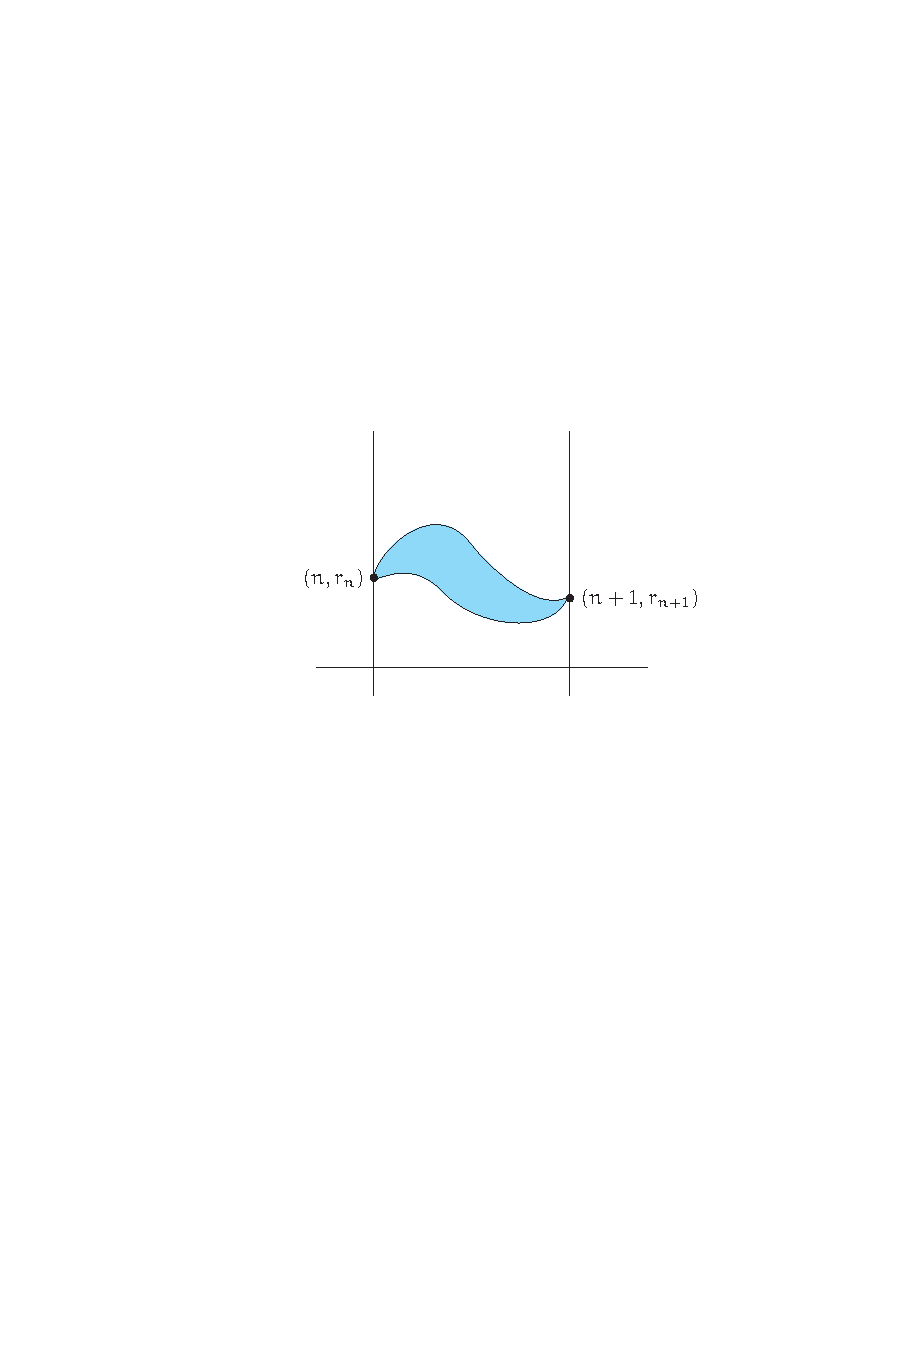
\includegraphics{pictures/quotient-product-no}
\caption{The open subset $A_n$.}
\end{figure}
\end{example}
On the other hand, we have the following result for coproducts.
\begin{proposition}\label{topological space coproduct of quotient map is quotient}
Let $(X_\alpha)_{\alpha\in A}$ and $(Y_\alpha)_{\alpha\in A}$ be topological spaces and for each $\alpha\in A$ let $p_\alpha:X_\alpha\to Y_\alpha$ be a quotient map. Then the map
\[p:\coprod_\alpha X_\alpha\to\coprod_\alpha Y_\alpha\]
which coincides with $p_\alpha$ on $X_\alpha$ is a quotient map.
\end{proposition}
\begin{proof}
Let $V$ be an subset in $\coprod_\alpha Y_\alpha$, then by the definition of $p$, we have
\[p^{-1}(V)=\bigcup_\alpha p_\alpha^{-1}(V\cap Y_\alpha),\]
so $p^{-1}(V)\cap X_\alpha=p_\alpha^{-1}(V\cap Y_\alpha)$. The claim now follows from by the definition of coproduct topology and the fact that each $p_\alpha$ is a quotient map.
\end{proof}
\subsection{Quotient space of a subspace}
Let $X$ be a topological space, $A$ a subspace of $X$, and $\pi$ the canonical map $X\to X/R$ of an equivalence relation $R$ on $X$. Let $R_A$ be the relation induced by $R$ on $A$, and $\pi|_A=\iota\circ\tilde{\pi}\circ\pi_A$ be the canonical decomposition of $\pi|_A$, so that we have a commutative diagram
\[\begin{tikzcd}
A\ar[rrr,bend right=20pt,swap,"\pi|_A"]\ar[r,"\pi_A"]&A/R_A\ar[r,"\tilde{\pi}"]&\pi(A)\ar[r,"\iota"]&X/R
\end{tikzcd}\]
\begin{proposition}\label{topological space quotient topology on subspace iff}
The canonical bijection $\tilde{\pi}:A/R_A\to\pi(A)$ is continuous. Furthermore, the following three statements are equivalent:
\begin{itemize}
\item[(\rmnum{1})] $\tilde{\pi}$ is a homeomorphism.
\item[(\rmnum{2})] Every open subset of $A$ which is saturated with respect to $R_A$ is the intersection with $A$ of an open subset of $X$ which is saturated with respect to $R$.
\item[(\rmnum{3})] Every closed subset of $A$ which is saturated with respect to $R_A$ is the intersection with $A$ of a closed subset of $X$ which is saturated with respect to $R$. 
\end{itemize}
\end{proposition}
\begin{proof}
Note that $A/R_A$ carries the quotient topology induced by $\pi_A$, and $\pi(A)$ carries the subspace topology induced by $X/R$. Now the claim follows from Proposition~\ref{topological space canonical decomposition homeomorphism iff}: if $U$ is an open subset of $A$ which is saturated with respect to $R_A$, and $\tilde{\pi}(U)=\pi(U)$ is the intersection with $\pi(A)$ of an open subset $V$ of $X/R$, then $U$ is the intersection with $A$ of the open subset $\pi^{-1}(V)$ of $X$, which is saturated with respect to $R$; and conversely, if $U$ is the intersection with $A$ of an open subset $W$ which is saturated with respect to $R$, then $\pi(U)$ is the intersection of $\pi(A)$ and $\pi(W)$, which is open in $X/R$.
\end{proof}
\begin{corollary}\label{topological space quotient map on saturated open set is quotient map}
If $A$ is an open (resp. closed) subset of $X$ which is saturated with respect to $R$, then the canonical mapping $\tilde{\pi}:A/R_A\to\pi(A)$ is a homeomorphism.
\end{corollary}
\begin{proof}
If $A$ is open (resp. closed) in $X$ and saturated with respect to $R$, and if $B\sub A$ is open (resp. closed) in $A$ and saturated with respect to $R_A$, then $B$ is open (resp. closed) in $X$ and saturated with respect to $R$.
\end{proof}
\begin{corollary}\label{topological space quotient map on sectioned orbit subspace}
If there is a continuous mapping $\varphi:X\to A$ such that $\varphi(x)\equiv x$ mod $R$ for each $x\in X$, then $\pi(A)=X/R$ and the canonical mapping $\tilde{\pi}:A/R_A\to X/R$ is a homeomorphism.
\end{corollary}
\begin{proof}
Since each equivalence class mod $R$ meets $A$, the canonical image of $\pi(A)$ in $X/R$ is the whole of $X/R$; on the other hand, if $U$ is open in $A$ and is saturated with respect to $R_A$, it follows from the hypothesis that $\varphi^{-1}(U)$ is the set obtained by saturating $U$ with respect to $R$; since $\varphi$ is continuous, $\varphi^{-1}(U)$ is open in $X$. The corollary follows from this fact by virtue of Proposition~\ref{topological space quotient topology on subspace iff}.
\end{proof}
\begin{example}
Let $R$ denote the equivalence relation $x=y$ mod $\Z$ on the real line $\R$ and let $I$ denote the closed interval $[0,1]$; $I$ contains at least one point of each equivalence class mod $R$. The canonical mapping of $I/R_I$ onto the torus $\T$ is a homeomorphism; for if $F$ is closed in $I$ (and hence in $\R$), in order to saturate $F$ with respect to the relation $R$ we have to take the union of the closed sets $F+n$ for all $n\in\Z$, which evidently form a locally finite family, so that their union is closed; the assertion follows from this. We remark that $I/R_I$ is obtained by identifying the points $0$ and $1$ in $I$.
\end{example}
\subsection{Hausdorff condition of quotient spaces}
Typically, to prove that a given quotient space is Hausdorff, one has to resort to the definition. For open quotient maps, however, we have the following criterion.
\begin{proposition}\label{quotient Hausdorff}
Suppose $q:X\to Y$ is an open quotient map. Then $Y$ is Hausdorff if and only if the set $\mathcal{R}:=\{(x_1,x_2):q(x_1)=q(x_2)\}$ is closed in $X\times X$.
\end{proposition}
\begin{proof}
First assume $Y$ is Hausdorff. If $(x_1,x_2)\notin\mathcal{R}$, then there are disjoint neighborhoods $V_1$ of $q(x_1)$ and $V_2$ of $q(x_2)$, and it follows that $q^{-1}(V_1)\times q^{-1}(V_2)$ is a neighborhood of $(x_1,x_2)$ that is disjoint from $\mathcal{R}$. Thus $\mathcal{R}$ is closed. (This implication does not require the assumption that $q$ is open.)\par
Conversely, assume $\mathcal{R}$ is closed. Given distinct points $y_1,y_2\in Y$, choose $x_1,x_2\in X$ such that $q(x_i)=y_i$. Because $(x_1,x_2)\notin\mathcal{R}$, there is a product neighborhood $U_1\times U_2$ of $(x_1,x_2)$ in $X\times X$ that is disjoint from $\mathcal{R}$. Since $q$ is open, $q(U_1)$ and $q(U_2)$ are disjoint neighborhoods of $y_1$ and $y_2$, respectively.
\end{proof}
\begin{corollary}
Suppose $\sim$ is an equivalence relation on a space $X$. If the quotient map $X\to X/$$\sim$ is an open map, then $X/$$\sim$ is Hausdorff if and only if $\sim$ is a closed subset of $X\times X$.
\end{corollary}
\begin{theorem}
Suppose $X$ is a compact Hausdorff space and $q:X\to Y$ is a quotient map. Then the following are equivalent.
\begin{itemize}
\item[(a)] $Y$ is Hausdorff.
\item[(b)] $q$ is a closed map.
\item[(c)] The set $\mathcal{R}=\{(x_1,x_2):q(x_1)=q(x_2)\}$ is closed in $X\times X$.
\end{itemize}
\end{theorem}
\begin{proof}
The implicaton $(a)\Rightarrow(b)$ is immediate by closed map lemma, and $(a)\Rightarrow(c)$ is proved just as in Proposition~\ref{quotient Hausdorff}. Next we prove $(b)\Rightarrow(a)$. Assuming $q$ is a closed map, we begin by showing that its fibers are compact. Every point $y\in Y$ is the image of some $x\in X$, and since $\{x\}$ is a closed subset of $X$, it follows that $\{y\}=q(\{x\})$ is a closed subset of $Y$. Thus by continuity, the fiber $q^{-1}(\{y\})$ is closed in $X$ and hence compact.\par 
To prove that $Y$ is Hausdorff, suppose $y_1$ and $y_2$ are distinct points of $Y$. Then we can prove the disjoint compact subsets $q^{-1}(y_1)$ and $q^{-1}(y_2)$ of $X$ have disjoint neighborhoods $U_1$ and $U_2$, respectively. Define subsets $W_1,W_2\sub Y$ by
\[W_i=Y-q(X-U_i)=\{y\in Y:q^{-1}(y)\sub U_i\}\]
Then $y_i\in W_i$ for each $i$ by construction, and $W_1$ and $W_2$ are disjoint because $U_1$ and $U_2$ are. To complete the proof, the fact that $q$ is closed implies that $W_i$ is open.\par
Finally, we prove $(c)\Rightarrow(a)$. Assuming that $\mathcal{R}$ is closed, we start again by showing that $q$ has compact fibers. Given $y\in Y$ and $x\notin q^{-1}(y)$, let $x_1$ be any point in $q^{-1}(y)$. (Such a point exists because $q$ is surjective.) Because $\mathcal{R}$ is closed and $(x,x_1)\notin\mathcal{R}$, there is a product neighborhood $U_1\times U_2$ of $(x_1,x)$ that is disjoint from $\mathcal{R}$. It follows that $U_2$ is a neighborhood of $x$ disjoint from $q^{-1}(y)$, for if $x_2$ were a point in $U_2\cap q^{-1}(y)$, then $(x_1,x_2)$ would lie in $\mathcal{R}\cap(U_1\times U_2)$, which is empty. Thus $q^{-1}(y)$ is closed in $X$ and hence compact.\par
Now let $y_1$ and $y_2$ be distinct points in $Y$. As before, there are disjoint open
subsets $U_1\sups q^{-1}(y_1)$ and $U_2\sups q^{-1}(y_2)$, and we define $W_1,W_2$ as before. These are disjoint sets containing $y_1$ and $y_2$, respectively, so we need only show they are open. Because $q$ is a quotient map, $W_i$ is open if and only if $q^{-1}(W_i)$ is open, which is the case if and only if $X-q^{-1}(W_i)$ is closed. From the definition of $W_i$, it follows that
\begin{align*}
X-q^{-1}(W_i)&=\{x\in X:q(x)\notin W_i\}=\{x\in X:q^{-1}(q(x))\nsubseteq U_i\}\\
&=\{x\in X:\text{$\exists x\in X-U_i$ such that $q(x)=q(x')$}\}\\
&=\pi_1(\mathcal{R}\cap(X\times X-U_i))
\end{align*}
where $\pi_1:X\times X\to X$ is the projection on the first factor. Observe that $\pi_1$ is a closed map by the closed map lemma. Our hypothesis on $\mathcal{R}$ implies that $\mathcal{R}\cap(X\times X-U_i)$ is closed in $X\times X$, and therefore $X-q^{-1}(W_i)$ is closed in $X$.
\end{proof}
\subsection{Direct limit of topological spaces}
Let $(X_\alpha)_{\alpha\in I}$ be a family of sets, and let $X$ be the set which is the coproduct of the $X_\alpha$. We shall identify each $X_\alpha$ with a subset of $X$ by means of the canonical injection $\iota_\alpha:X_\alpha\to X$.\par
Let $R$ be an equivalence relation on $X$ such that each equivalence class of $R$ has at most one element in each $X_\alpha$; for each pair of indices $(\alpha,\beta)$ let $A_{\alpha\beta}$ be the subset of $X_\alpha$ consisting of the elements $x$ for which there is an element $y\in X_{\beta}$ which belongs to the equivalence class of $x$. Clearly to each $x\in A_{\alpha\beta}$ there is a unique $y\in X_\beta$ which is congruent to $x$ mod $R$; the mappings $\phi_{\beta\alpha}:A_{\alpha\beta}\to A_{\beta\alpha}$ so defined satisfy the following conditions:
\begin{itemize}
\item[(a)] For each $\alpha\in I$, $\phi_{\alpha\alpha}$ is the identity mapping of $A_{\alpha\alpha}=X_\alpha$.
\item[(b)] For each triple of indices $(\alpha,\beta,\gamma)$ of $I$ and each $x\in A_{\alpha\beta}\cap A_{\alpha\gamma}$, we have $\phi_{\beta\alpha}(x)\in A_{\beta\gamma}$ and $\phi_{\gamma\alpha}(x)=\phi_{\gamma\beta}(\phi_{\beta\alpha}(x))$.
\end{itemize}

Conversely, suppose that for each pair of indices $(\alpha,\beta)$ we are given a subset $A_{\alpha\beta}$ of $X_\alpha$ and a mapping $\phi_{\beta\alpha}:A_{\alpha\beta}\to A_{\beta\alpha}$ satisfying the conditions (a) and (b) above. It follows first of all from (b) applied to the triples $(\alpha,\beta,\alpha)$ and $(\beta,\alpha,\beta)$ that $\phi_{\alpha\beta}\circ\phi_{\beta\alpha}$ (resp. $\phi_{\beta\alpha}\circ\phi_{\alpha\beta}$) is the restriction of $\phi_{\alpha\alpha}$ (resp. $\phi_{\beta\beta}$) to $A_{\alpha\alpha}$ (resp. $A_{\beta\beta}$); hence we deduce from (a) that $\phi_{\beta\alpha}$ and $\phi_{\alpha\beta}$ are bijections which are mverses of each other. Now let $R$ be the relation "there exist $\alpha,\beta$ such that $x\in A_{\alpha\beta}$, $y\in A_{\beta\alpha}$ and $y=\phi_{\beta\alpha}(x)$". It follows from (a) and what precedes that $R$ is reflexive and symmetric; on the other hand, if 
\[x\in A_{\alpha\beta},\quad y=\phi_{\beta\alpha}(x)\in A_{\beta\alpha}\cap A_{\beta\gamma},\quad z=\phi_{\gamma\beta}(y)\in A_{\gamma\beta},\]
then also $x=\phi_{\alpha\beta}(y)$ and by (b) we have $z=\phi_{\gamma\alpha}(x)$; thus $R$ is transitive, and so is an equivalence relation on $X$. It follows also from (a) and from the definition of $R$ that each equivalence class mod $R$ has at most one element in each of the sets $X_\alpha$, and that $A_{\alpha\beta}$ is the set of all $x\in X_\alpha$ for which there is an element $y\in X_\beta$ congruent to $x$ mod $R$. We say that the quotient set $X/R$ is obtained by pasting together the $X_\alpha$ along the $A_{\alpha\beta}$ by means of the bijections $\phi_{\beta\alpha}$. If $\pi:X\to X/R$ is the canonical mapping, the restriction of $\pi$ to each $X_\alpha$ is a bijection of $X_\alpha$ onto $\pi(X_\alpha)$.\par
Now suppose that each $X_\alpha$ is a topological space, and let $\mathcal{T}_\alpha$ be its topology. Let $\mathcal{T}$ be the finest topology on the set $X/R$ for which the mappings $\pi\circ\iota_\alpha$ are continuous; then $\mathcal{T}$ is the quotient by $R$ of the topology on $X$ which is the coproduct of the topologies $\mathcal{T}_\alpha$. We say that the topological space $X/R$ (with the topology $\mathcal{T}$) is obtained by pasting together the topological spaces $X_\alpha$ along the $A_{\alpha\beta}$ by means of the bijections $\phi_{\beta\alpha}$. The open (resp. closed) subsets of $X/R$ are thus the canonical images of the subsets $B$ of $X$ which are saturated with respect to $R$ and are such that $B\cap X_\alpha$ is open (resp. closed) in $X_\alpha$ for each $\alpha\in I$.\par
Since the restriction of $\pi$ to each $X_\alpha$ is a bijection onto the subset $\pi(X_\alpha)$ of $X/R$, we can transport the topology $\mathcal{T}_\alpha$ to $\pi(X_\alpha)$ by means of this bijection, so that $\pi(X_\alpha)$ carries a topology $\widetilde{\mathcal{T}}_\alpha$ and the topology $\mathcal{T}$ on $X/R$ is the finest for which the canonical injections $\pi(X_\alpha)\to X/R$ are continuous. In general, the topology induced by $\mathcal{T}$ on $\pi(X_\alpha)$ is coarser than $\widetilde{\mathcal{T}}_\alpha$, but not identical with the latter; even if the $\phi_{\beta\alpha}$ are homeomorphisms. However, it follows from Proposition~\ref{topological space pasting topology} that, with the preceding notation:
\begin{proposition}
Suppose that the $\phi_{\beta\alpha}$ are homeomorphisms and that each $A_{\alpha\beta}$ is open (resp. closed) in $X_\alpha$; then each $\pi(X_\alpha)$ is open (resp. closed) in $X/R$ and the restriction of $\pi$ to $X_\alpha$ is a homeomorphism of $X_\alpha$ onto the subspace $\pi(X_\alpha)$ of $X/R$.
\end{proposition}
\section{Product of topological spaces}
\subsection{Product spaces}
\begin{definition}
Given a family $(X_i)_{i\in I}$ of topological spaces, the \textbf{product space} of this family is the product set $X=\prod_{i\in I}X_i$ with the initial topology induced by the projections $\pi_i:X\to X_i$. The spaces $X_i$ are called the factors of $X$.
\end{definition}
By virtue of Proposition~\ref{topological space initial topology definition}, the product topology on $X$ has as a base the set of finite intersections of sets of the form $\pi_i^{-1}(U_i)$, where $U_i$ is open in $X_i$; these sets are products $\prod_{i\in I}U_i$, where $U_i$ is open in $X_i$ for each $i$ and $U_i=X_i$ for all but a finite number of indices These sets will be called \textbf{elementary sets}.\par
If $\mathcal{B}_i$ is a base of the topology of $X_i$ for each $i\in I$, it is clear that the elementary sets $\prod_iB_i$ such that $B_i=X_i$ for all but finitely many indices form another base of the product topology. The elementary sets of this type which contain a given point $x\in X$ thus form a fundamental system of neighbourhoods of $x$.\par
If $I$ is a finite set, the construction of the product topology from the topologies of the factors $X_i$ is simpler: the elementary sets are just products $\prod_{i\in I}U_i$ where $U_i$ is any open subset of $X_i$ for each $i\in I$.
\begin{example}
The product $\R^n$ of $n$ spaces identical with the real line $\R$ is called real number space of $n$ dimensions; $\R^2$ is also called the real plane. Likewise, starting from the rational line $\Q$, we define the rational number space of $n$ dimensions $\Q^n$ (rational plane for $n=2$). The topology of the space $\R^n$ has as a base the set of all products of $n$ open intervals in $\R$, which are called open boxes of $n$ dimensions. The open boxes which contain a point $x\in\R^n$ form a fundamental system of neighbourhoods of this point. Likewise the products of $n$ closed intervals in $\R$ are called closed boxes of $n$ dimensions. The closed boxes to which $x$ is interior also form a fundamental system of neighbourhoods of $x$. There are analogous results for $\Q^n$.
\end{example}
\begin{proposition}\label{topological space map into product continuous iff}
Let $f=(f_i)$ be a mapping of a topological space $Y$ into a product space $X=\prod_{i\in I}X_i$. Then $f$ is continuous at a point $y\in Y$ if and onlY if $f_i$ is continuous at $y$ for each $i\in I$.
\end{proposition}
\begin{proof}
Since $f_i=f\circ\pi_i$, this is a special case of Proposition~\ref{topological space initial topology definition}.
\end{proof}
\begin{corollary}\label{topological product map continuous iff}
Let $(X_i)_{i\in I}$ and $(Y_i)_{i\in I}$ be two families of topological spaces with tke same set of indices. For each $i\in I$, let $f_i$ be a mapping of $X_i$ into $Y_i$. In order that the product mapping $f:(x_i)\to(f_i(x_i))$ should be continuous at a point $a=(a_i)$, it is necessary and sufficient that $f_i$ is continuous at $a_i$ for each $i\in I$.
\end{corollary}
\begin{proof}
The map $f$ can be written as $x\mapsto(f_i(\pi_i(x)))$, so that by Proposition~\ref{topological space map into product continuous iff} the condition is sufficient. Conversely, for each $j\in I$ let $g_j$ be the mapping of $X_j$ into $\prod_{i\in I}X_i$ such that $\pi_j(g_j(x))=x_j$ and $\pi_i(g_j(x))=a_i$ for $i\neq j$. Then $g_j$ is continuous at the point $a_j$, by Proposition~\ref{topological space map into product continuous iff}. Since $f_j=\pi_j\circ f\circ g_j$, it follows that if $f$ is continuous at $a$ then $f_j$ is continuous at $a_j$.
\end{proof}
\begin{corollary}
Let $X$, $Y$ be two topological spaces. In order that a mapping $f:X\to Y$ should be continuous it is necessary and sufficient that the mapping $g:x\mapsto(x,f(x))$ is a homeomorphism of $X$ onto the graph $\Gamma(f)$ (considered as a subspace of the product space $X\times Y$).
\end{corollary}
\begin{proof}
Since $f=\pi_2\circ g$, the condition is sufficient. It is also necessary, for if $f$ is continuous, then $g$ is bijective and continuous (Proposition~\ref{topological space map into product continuous iff}) and the inverse of $g$ is the restriction of $\pi_1$ to $\Gamma(f)$, which is continuous.
\end{proof}
\begin{proposition}[\textbf{Associativity of topological products}]
Let $(X_i)_{i\in I}$ be a family of topological spaces, $(I_\kappa)_{\kappa\in K}$ a partition of the set $I$, and for each $\kappa\in K$ let $X_\kappa=\prod_{i\in I_\kappa}X_i$. Then the canonical mapping of the product space $\prod_{i\in I}X_i$ onto the product space $\prod_{\kappa\in K}X_\kappa$ is a homeomorphism.
\end{proposition}
\begin{proof}
This is a special case of the transitivity of initial topologies.
\end{proof}
\begin{corollary}
Let $\sigma\in\mathfrak{S}_I$ be a permutation of the set $I$. Then the mapping $(x_i)\mapsto(x_{\sigma(i)})$ is a homeomorphism of $\prod_{i\in I}$ onto $\prod_{i\in I}X_{\sigma(i)}$.
\end{corollary}
\begin{proof}
Take $K=I$ and $I_i=\{\sigma(i)\}$ in the previous proposition.
\end{proof}
Finally, we show that, the general concept of initial topologies can be defined using product spaces and product topology.
\begin{proposition}\label{topological space initial topology defined by product}
Let $X$ be a set, $(Y_i)_{i\in I}$ a family of topological spaces, and for each $i\in I$ let $f_i$ be a mapping of $X$ into $Y_i$. Let $f$ be the mapping $x\mapsto(f_i(x))$ of $X$ into $Y=\prod_{i\in I}Y_i$. Then the initial topology on $X$ induced by $(f_i)$ is the inverse image under $f$ of the topology induced on $f(X)$ by the product topology on $Y$.
\end{proposition}
\begin{proof}
This is another application of the transitivity of initial topologies.
\end{proof}
\begin{corollary}
For each $i\in I$ let $A_i$ be a subspace of $X_i$. Then the topology induced on $A=\prod_{i\in I}A_i$ by the product topology on $\prod_{i\in I}X_i$ is the product of the topologies of the subspaces $A_i$.
\end{corollary}
\begin{proof}
Let $\iota_i$ be the canonical injection $A_i\to X_i$ and apply Proposition~\ref{topological space initial topology defined by product} to the mappings $f_i=\iota_i\circ\pi_i$.
\end{proof}
There is another topology on the product space $X=\prod_{i\in I}X_i$ called the box topology, whose open sets are defined to be the product of open subsets in $X_i$. The box topology turns out to have too many open sets, for example, Proposition~\ref{topological space map into product continuous iff} does not hold for it.
\begin{example}
Consider $\R^\omega$, the countably infinite product of $\R$ with itself. That is, $\R^\omega=\prod_{n\in\Z_+}X_n$, where $X_n=\R$ for each $n$. Let us define a function $f:\R\to\R^\omega$ by the equation
\[f(x)=(x,x,\dots,x,\dots).\]
Each of the coordinate functions $f_n:\R\to\R$ is continuous; therefore, the function $f$ is continuous if $\R^\omega$ is given the product topology. But $f$ is not continuous if $\R^\omega$ is given the box topology. Consider, for example, the basis element
\[B=\prod_{n\in\Z_+}(-1/n,1/n),\]
for the box topology. We assert that $f^{-1}(B)$ is not open in $\R$: If $f^{-1}(B)$ contains some interval $(-\delta,\delta)$ about the point $0$, then we must have $(-\delta,\delta)\sub(-1/n,1/n)$ for each $n$, whence $\delta=0$, a contradiction.
\end{example}
\subsection{Sections and projections}
\begin{proposition}\label{topological space section map homeomorphism}
Let $X$ and $Y$ be topological spaces. Then
\begin{itemize}
\item[(a)] for each $a\in X$, the map $y\mapsto(a,y)$ is a homeomorphism from $Y$ to the subspace $\{a\}\times Y$ of $X\times Y$;
\item[(b)] for each $b\in Y$, the map $x\mapsto(x,b)$ is a homeomorphism from $X$ to the subspace $X\times\{b\}$ of $X\times Y$.
\end{itemize}
\end{proposition}
\begin{proof}
Since $\pi_Y$, restricted to $\{a\}\times Y$, is a continuous inverse of the given map in (a), this is a particular case of Corollary~\ref{topological product map continuous iff} applied to the constant function $x\mapsto a$. The same proof applies to (b).
\end{proof}
Note that the mapping $y\mapsto(a,y)$ is a continuous section with respect to the equivalence relation $\pi_X(z)=\pi_X(z')$ in $X\times Y$; the quotient space of $X\times Y$ by this equivalence relation is therefore homeomorphic to $Y$.
\begin{corollary}\label{topological space section of open close}
The section $A(x)$ of an open (resp. closed) set $A$ of the product $X\times Y$ at an arbitrary point $x\in X$ is open (resp. closed) in $Y$.
\end{corollary}
Using Proposition~\ref{topological product map continuous iff}, we also get the following useful fact.
\begin{proposition}\label{topological space projection is open}
The projection of $X\times Y$ onto either factor is an open map.
\end{proposition}
\begin{proof}
Let $U$ be open in $X\times Y$, then we have 
\[\pi_X(U)=\bigcup_{y\in Y}U(y),\quad\pi_Y(U)=\bigcup_{x\in X}U(x),\]
and the proposition follows from the Corollary~\ref{topological space section of open close}.
\end{proof}
Note that the projection of a closed subset of $X\times Y$ onto a factor need not be closed. For example, in the real plane $\R^2$, the hyperbola whose equation is $xy=1$ is a closed set, but both its projections are equal to the complement of the point $0$ in $\R$. and this is not a closed set.
\begin{proposition}\label{topological space continuous is separately conitnuous}
Let $X$, $Y$ and $Z$ be three topological spaces, $f$ a mapping of the product space $X\times Y$ into $Z$. If $f$ is continuous at the point $(a,b)\in X\times Y$, then the partial mapping $y\mapsto f(a,y)$ of $Y$ into $Z$ is continuous at the point $b$.
\end{proposition}
\begin{proof}
This mapping is the composition of $f$ and the mapping $y\mapsto(a,y)$; hence the result follows from Proposition~\ref{topological space section map homeomorphism}.
\end{proof}
Proposition~\ref{topological space continuous is separately conitnuous} is often expressed by saying that a continuous function of two variables is continuous with respect to each of them separately.
\begin{example}
It is possible for all the partial mappings determined by a map $f:X\times Y\to Z$ to be continuous without $f$ being continuous. For example if $f$ is the mapping of the real plane $\R^2$ into $\R$ defined by
\[f(x,y)=\begin{cases}
\dfrac{xy}{x^2+y^2}&(x,y)\neq(0,0),\\
0&(x,y)=(0,0).
\end{cases}\]
Then all the partial mappings are continuous; but $f$ is not continuous at $(0,0)$.
\end{example}
\begin{proposition}\label{topological space closure of product subspace}
In a product space $\prod_{i\in I}X_i$ the closure of a product of sets $\prod_{i\in I}A_i$ is the same as the product $A_i$ of their closures.
\end{proposition}
\begin{proof}
Suppose that $a=(a_i)$ lies in the closure of $\prod_{i\in I}A_i$; then for each $j\in I$, $a_j=\pi_j(a)$ is in the closure of $A_j$ because of the continuity of $\pi_j$ and therefore $a\in\prod_{i\in I}\widebar{A}_i$. Conversely, let $b=(b_i)\in\prod_{i\in I}\widebar{A}_i$ and let $\prod_{i\in I}U_i$ be any elementary set containing $b$; for each $i\in I$, $U_i$ contains a point $x_i\in A_i$; hence $\prod_{i\in I}U_i$ contains the point $(x_i)\in\prod_{i\in I}A_i$ and therefore $b$ lies in the closure of $\prod_{i\in I}A_i$.
\end{proof}
\begin{corollary}
A product $\prod_{i\in I}A_i$ of non-empty sets is closed in the product space $\prod_{i\in I}$ if and only if $A_i$ is closed in $X_i$ for each $i\in I$.
\end{corollary}
\begin{remark}
Note that if $I$ is finite, a product $\prod_{i\in I}A_i$ is open provided that $A_i$ is open in $X_i$ for each $i\in I$; but this is no longer so if $I$ is infinite.
\end{remark}
As an application of Proposition~\ref{topological space closure of product subspace}, we give a certain family of dense subsets in a product space.
\begin{proposition}\label{topological space dense subset in product}
Let $a=(a_i)$ be any point of a product space $X=\prod_{i\in I}X_i$; then the set $D$ of points $x\in X$ such that $\pi_i(x)=a_i$ except for a finite number of indices $i$ is dense in $X$.
\end{proposition}
\begin{proof}
For each $x\in X$ and each elementary set $U=\prod_{i\in I}U_i$ which contains $x$, we have $U_i=X_i$ except for indices $i$ belonging to a finite subset of $J$; if we take $y_i=x_i$ for $i\notin J$ and $y_i=a_i$ for $i\in J$, it is clear that $y=(y_i)\in D$ and $y\in U$; hence the result.
\end{proof}
\subsection{Inverse limit of topological spaces}
Let $I$ be a partially ordered (but not necessarily directed) set, in which the order relation is written as $\preceq$. For each $\alpha\in I$, let $X_\alpha$ be a topological space, and for each pair $(\alpha,\beta)$ such that $\alpha\preceq\beta$ let $f_{\alpha\beta}$ be a mapping of $X_\beta$ into $X_\alpha$. We say that $(X_\alpha,f_{\alpha\beta})$ is an inverse system of topological spaces if:
\begin{itemize}
\item[(a)] $(X_\alpha,f_{\alpha\beta}$) is an inverse system of sets;
\item[(b)] Each $f_{\alpha\beta}$ is continuous. 
\end{itemize} 
Let $X$ denote the set $\llim X_\alpha$ and for each $\alpha\in I$ let $f_\alpha$ be the canonical mapping $X\to X_\alpha$; then the initial topology induced by the $f_\alpha$'s is said to be the inverse limit (with respect to the $f_{\alpha\beta}$) of the topologies of the $X_\alpha$ and the set $X$ with this topology is called the inverse limit of the inverse system of topological spaces $(X_\alpha,f_{\alpha\beta})$. Whenever we speak of $\llim X_\alpha$ as a topological space, it is always to be understood that the topology of this space is the inverse limit of the topologies of the $X_\alpha$ unless the contrary is expressly stated.\par
The set $X$ is the subset of the product $\prod_{\alpha}X_\alpha$ consisting of those points $x$ such that
\[\pi_\alpha(x)=f_{\alpha\beta}(\pi_\beta(x)).\]
whenever $\alpha\preceq\beta$. It follows from Proposition~\ref{topological space initial topology defined by product} that the inverse limit of the topologies of the $X_\alpha$ is the same as the topology induced on $X$ by the topology of the product space $\prod_\alpha X_\alpha$. If, for each $\alpha\in I$, $A_\alpha$ is a subspace of $X_\alpha$ such that the $(A_\alpha,f_{\alpha\beta}|_{A_\beta})$ form an inverse system of subsets of the $X_\alpha$, then it is clear that the topological space $\llim A_\alpha$ is a subspace of $\llim X_\alpha$.\par
Let $(Y_\alpha,g_{\alpha\beta})$ be another inverse system of topological spaces indexed by the same set $I$, and for each $\alpha\in I$ let $\varphi_\alpha:X_\alpha\to Y_\alpha$ be a continuous mapping such that $(\varphi_\alpha)$ is an inverse system of mappings; then $\varphi=\llim \varphi_\alpha$ is a continuous mapping of $X=\llim X_\alpha$ into $Y=\llim Y_\alpha$. For if $g_\alpha$ is the canonical mapping $Y\to Y_\alpha$, we have $g_\alpha\circ\varphi=\varphi_\alpha\circ f_\alpha$, so that $g_\alpha\circ\varphi$ is continuous for each $\alpha\in I$, and so $\varphi$ is continuous.\par
Finally, suppose $I$ is a directed set, and let $J$ be a cofinal subset of $I$; let $\widetilde{X}$ be the inverse limit of the inverse system of topological spaces $(X_\alpha,f_{\alpha\beta})_{\alpha,\beta\in J}$. Then the canonical bijection $\psi:X\to\widetilde{X}$ is a homeomorphism. For we have $\pi_\alpha(\psi(x))=\pi_\alpha(x)$ for each $\alpha\in J$, hence $\psi$ is continuous; and if $\phi$ is the inverse of $\psi$, then for each $\alpha\in I$ there exists $\beta\in J$ such that $\alpha\preceq\beta$, and therefore $\pi_\alpha(\phi(z))=f_{\alpha\beta}(\pi_\beta(z))$, which shows that $\phi$ is continuous, since the $f_{\alpha\beta}$'s are continuous.
\begin{proposition}\label{topological space inverse limit cofinal system base}
Let $I$ be a directed set and $J$ a cofinal subset of $I$. Let $(X_\alpha,f_{\alpha\beta})$ be an inverse system of topological spaces indexed by $I$; let $X=\llim X_\alpha$ and let $f_\alpha:X\to X_\alpha$ be the canonical mapping. Then the family of sets $f_\alpha^{-1}(U_\alpha)$, where $\alpha$ runs through $J$ and $U_\alpha$ runs through a base $\mathcal{B}_\alpha$ of the topology of $X_\alpha$ for each $\alpha\in J$, is a base of the topology of $X$.
\end{proposition}
\begin{proof}
We know that the finite intersections of sets of the form $f_\alpha^{-1}(U_\alpha)$, $\alpha\in I$, $U_\alpha$ open in $X_\alpha$ form a base of the topology of $X$. If $\alpha_1,\dots,\alpha_n$ is a finite family of indices of $I$, then there exists $\beta\in J$ such that $\alpha_i\preceq\beta$ for $1\leq i\leq n$; hence $f_{\alpha_i}=f_{\alpha_i\beta}\circ f_\beta$; if we put $U_\beta=\bigcap_{i=1}^{n}f_{\alpha_i\beta}^{-1}(U_{\alpha_i})$, then
\[f_\beta^{-1}(U_\beta)=\bigcap_{i=1}^{n}f_{\alpha_i}^{-1}(U_{\alpha_i}).\]
But $U_\beta$ is open and is therefore a union of sets belonging to $\mathcal{B}_\beta$. Hence the result.
\end{proof}
\begin{corollary}
Let $A$ be a subset of $X$ and let $A_\alpha=f_\alpha(A)$ for each $\alpha\in I$. Then:
\begin{itemize}
\item[(a)] The $A_\alpha$ (resp. the $\widebar{A}_\alpha$) form an inverse system of subsets of the $X_\alpha$, and $\widebar{A}=\bigcap_{\alpha}f_\alpha^{-1}(\widebar{A}_\alpha)=\llim\widebar{A}_\alpha$.
\item[(b)] If $A$ is closed in $X$ then $A=\llim A_\alpha=\llim \widebar{A}_\alpha$.
\end{itemize}
\end{corollary}
\begin{proof}
The first assertion of (a) follows from the relations $f_\alpha=f_{\alpha\beta}\circ f_\beta$ for $\alpha\preceq\beta$ and from the continuity of the $f_\alpha$. Let $A'$ denote $\bigcap_{\alpha}f_\alpha^{-1}(\widebar{A}_\alpha)$, then it is clear that $A'$ is closed and contains $A$, so that $\widebar{A}\sub A'$. Conversely, let $x\in A'$; we have to show that $x$ lies in the closure of $A$. By virtue of Proposition~\ref{topological space inverse limit cofinal system base}, it is enough to prove that every neighbourhood of $x$ which is of the form $f_\alpha^{-1}(U_\alpha)$, with $\alpha\in I$ and $U_\alpha$ open in $X_\alpha$ meets $A$. Now, by hypothesis, $f_\alpha(x)\in U_\alpha$, and since $f_\alpha(x)\in \widebar{A}_\alpha$ we have $U_\alpha\cap A_\alpha\neq\emp$, which means $A\cap f_\alpha^{-1}(A_\alpha)\neq\emp$.\par
To establish (b) it is enough to remark that, without any restriction on $A$, we have $A\sub\llim A_\alpha\sub\llim\widebar{A}_\alpha$; now if $A$ is closed, then from (a) we have $A=\llim\widebar{A}_\alpha$, so the claim follows.
\end{proof}
\begin{example}
Let $I$ be a directed set and $(X_\alpha)_{\alpha\in I}$ a family of subsets of a set $Y$, such that $X_\alpha\sups X_\beta$ whenever $\alpha\preceq\beta$. For each $\alpha\in I$ let $\mathcal{T}_\alpha$ be a topology on $X_\alpha$ such that $\mathcal{T}_\alpha$ is finer than the topology induced on $X_\alpha$ by $\mathcal{T}_\beta$ whenever $\alpha\preceq\beta$. If we take $f_{\alpha\beta}$ to be the canonical injection $X_\beta\to X_\alpha$ for $\alpha\preceq\beta$, then $\llim X_\alpha$ may be identified canonically with the intersection $X$ of the $X_\alpha$, with the topology which is the least upper bound of the topologies induced on $X$ by the $\mathcal{T}_\alpha$.
\end{example}
\section{Connectedness}
\subsection{Connected spaces}
The definition of connectedness for a topological space is a quite natural one. One says that a space can be "separated" if it can be broken up into two "globs"--disjoint open sets. Otherwise, one says that it is connected. From this simple idea much follows.
\begin{definition}
Let $X$ be a topological space. A \textbf{separation} of $X$ is a pair $U$, $V$ of disjoint nonempty open subsets of $X$ whose union is $X$. The space $X$ is said to be connected if there does not exist a separation of $X$.
\end{definition}
Connectedness is obviously a topological property, since it is formulated entirely in terms of the collection of open sets of $X$. Said differently, if $X$ is connected, so is any space homeomorphic to $X$.\par
For a subspace $A$ of a topological space $X$, there is another useful way of formulating the definition of connectedness:
\begin{lemma}\label{topological space connectedness of subspace}
If $A$ is a subspace of $X$, a separation of $A$ is a pair of disjoint nonempty sets $U$ and $V$ whose union is $A$, neither of which contains a limit point of the other. The space $A$ is connected if there exists no separation of $A$.
\end{lemma}
\begin{proof}
Suppose first that $U$ and $V$ form a separation of $A$. Then $U$ is both open and closed in $A$. The closure of $U$ in $A$ is the set $\widebar{U}\cap A$ (where $\widebar{U}$ as usual denotes the closure of $U$ in $X$). Since $U$ is closed in $A$, $U=\widebar{U}\cap A$; or to say the same thing, $\widebar{U}\cap V=\emp$. Since $\widebar{U}$ is the union of $U$ and its limit points, $V$ contains no limit points of $U$. A similar argument shows that $U$ contains no limit points of $V$.\par
Conversely, suppose that $U$ and $V$ are disjoint nonempty sets whose union is $A$, neither of which contains a limit point of the other. Then $\widebar{U}\cap V=\emp$ and $\widebar{V}\cap U=\emp$; therefore, we conclude that $\widebar{U}\cap A=U$ and $\widebar{V}\cap A=V$. Thus both $U$ and $V$ are closed in $A$, and since $U\cup V=A$, they are open in $A$ as well.
\end{proof}
\begin{example}
Let $X$ denote a two-point space in the indiscrete topology. Obviously there is no separation of $X$, so $X$ is connected.
\end{example}
\begin{example}
Let $A$ denote the subspace $[-1,0)\cup(0,1]$ of the real line $\R$. Each of the sets $[-1,0)$ and $(0,1]$ is nonempty and open in $A$ (although not in $\R$); therefore, they form a separation of $A$. Alternatively, note that neither of these sets contains a limit point of the other. (They do have a limit point $0$ in common, but that does not matter.)
\end{example}
\begin{example}
A subspace of $\mathbb{R}$ is connected if and only if it is an interval: Clearly intervals are connected. Now suppose $X$ is connected in $\R$ and is not an interval. Then there are $x,y\in X$ and $z\notin X$ such that $x<z<y$. We set
\[O_1=(-\infty,z)\cap X,\quad O_2=X\cap(z,+\infty)\]
Then $O_1$ and $O_2$ is a separation of $X$, and since $x\in O_1$, $y\in O_2$ they are both nonempty. This is a contradiction since $X$ is connected, hence $X$ is an interval.
\end{example}
\begin{example}
Let $X$ be the subspace $[-1,1]$ of the real line. The sets $[-1,0]$ and $(0,1]$ are disjoint and nonempty, but they do not form a separation of $X$, because the first set is not open in $X$. Alternatively, note that the first set contains a limit point, $0$, of the second. Indeed, there exists no separation of the space $[-1,1]$.
\end{example}
\begin{example}
The rationals $\Q$ are not connected. Indeed, the only connected subspaces of $\Q$ are the one-point sets: If $A$ is a subspace of $\Q$ containing two points $p$ and $q$, one can choose an irrational number $\alpha$ lying between $p$ and $q$, and write $A$ as the union of the open sets
\[A=(A\cap(-\infty,\alpha))\cup(A\cap(\alpha,+\infty)).\]
\end{example}
\begin{example}
Consider the following subset of the plane $\R^2$:
\[X=\{(x,y)\in\R^2:y=0\}\cup\{(x,y):\text{$x>0$ and $xy=1$}\}.\]
Then $X$ is not connected; indeed, the two indicated sets form a separation of $X$ because neither contains a limit point of the other.
\end{example}
We have given several examples of spaces that are not connected. How can one construct spaces that are connected? We shall now prove some useful properties of connectedness, and later use them to construct connected topological spaces. First, we give another criterion for connectedness which is quite simple but useful.
\begin{proposition}\label{topological space connected iff continuous map to {0,1}}
A topological space $X$ is connected if and only if every continuous map $f:X\to\{0,1\}$ is constant, with the space $\{0,1\}$ given the discrete topology.
\end{proposition}
\begin{proof}
Clearly if $f$ is not constant then $f^{-1}(0)\cup f^{-1}(1)$ is a separation of $X$. Conversely, if $U$ and $V$ form a separation of $X$ then the characteristic function $\chi_U$ is nonconstant and continuous.
\end{proof}
\begin{proposition}[\textbf{Properties of Connected Spaces}]\label{topological space connected prop}
Let $X$ be a topological space.
\begin{itemize}
\item[(a)] Suppose that $U,V$ are disjoint open subsets of $X$. If $A$ is a connected subset of $X$ contained in $U\cup V$, then either $A\sub U$ or $A\sub V$.
\item[(b)] Suppose $X$ is any space and $A\sub X$ is connected. If $B$ is a subset such that $A\sub B\sub\widebar{A}$, then it is connected. In particular, $\widebar{A}$ is connected.
\item[(c)] Let $\{C_{\alpha}\}_{\alpha\in I}$ be a collection of connected subspaces of $X$ with a point in common. Then $\bigcup_{\alpha\in I}C_\alpha$ is connected.
\item[(d)] Let $\{C_{\alpha}\}_{\alpha\in I}$ be a collection of connected subspaces of $X$ with $C_\alpha\cap C_\beta\neq\emp$ for all $\alpha,\beta\in I$. Then $\bigcup_{\alpha\in I}C_\alpha$ is connected. 
\end{itemize}
\end{proposition}
\begin{proof}
For (a), if $A$ contained points in both $U$ and $V$, then $A\cap U$ and $A\cap V$ would form a separation of $A$. To prove (b), suppose $A$ is connected and $A\sub B\sub\widebar{A}$. Suppose that $B=U\cup V$ is a separation of $B$. By part (a), the set $A$ must lie entirely in $U$ or in $V$; say $A\sub U$. Then $\widebar{A}\sub\widebar{U}$; since $\widebar{U}$ and $V$ are disjoint, $B$ cannot intersect $V$. This contradicts the fact that $V$ is a nonempty subset of $B$.\par
For part (c), let $p$ be a point that is contained in $C_\alpha$ for every $\alpha$, and let $f:\bigcup_\alpha C_\alpha\to\{0,1\}$ be a continuous function. Then $f$ is constant when restricted to each $C_\alpha$, since $C_\alpha$ is connected. Since $C_\alpha$ contains $p$ for each $\alpha$, it then follows that $f$ is constant. This shows $\bigcup_{\alpha}C_\alpha$ is connected. Part (c) can be proved similarly.
\end{proof}
\begin{corollary}
Let $X$ be a topological space and $(A_n)_{n\in\N}$ be an infinite sequence of connected subspaces such that $A_n\cap A_{n+1}\neq\emp$ for all $n\geq 0$. Then the union $\bigcup_nA_n$ is connected.
\end{corollary}
\begin{proof}
By induction on $n$ we see immediately that the set $B_n=\bigcup_{i=1}^{n}A_i$ is connected for all $n$, by Proposition~\ref{topological space connected prop}. The sets $B_n$ have a non-empty intersection; hence their union, equal to $\bigcup_nB_n$, is connected by Proposition~\ref{topological space connected prop}.
\end{proof}
\begin{proposition}\label{topological space connected continuous image}
The image of a connected space under a continuous map is connected.
\end{proposition}
\begin{proof}
Let $f:X\to Y$ be a continuous map; let $X$ be connected. We wish to prove the image space $f(X)$ is connected. Since the map obtained from $f$ by restricting its range to the space is also continuous, it suffices to consider the case that $f$ is surjective. Suppose that $Y=U\cup V$ is a separation of $Y$ into two disjoint nonempty sets open in $Y$. Then $f^{-1}(U)$ and $f^{-1}(V)$ are disjoint sets whose union is $X$; they are open in $X$ because $f$ is continuous, and nonempty because $f$ is surjective. Therefore, they form a separation of $X$, contradicting the assumption that $X$ is connected.
\end{proof}
\begin{corollary}\label{topological space quotient of connected space}
Every quotient space of a connected space is connected.
\end{corollary}
As for Corollary~\ref{topological space quotient of connected space}, we have the following converse.
\begin{proposition}\label{topological space connected if quotient is}
Let $X$ be a topological space and $R$ an equivalence relation on $X$. If the quotient space $X/R$ is connected, and if each equivalence class of $R$ is connected, then $X$ is connected.
\end{proposition}
\begin{proof}
Suppose $X$ is not connected. Then there is a partition of $X$ into two open sets $U$, $V$. The sets $U$, $V$ are saturated with respect to $R$ in view of Proposition~\ref{topological space connected prop}(a). The canonical images of $U$ and $V$ are therefore open sets in $X/R$ and form a partition of $X/R$; this contradicts the assumption that $X/R$ is connected.
\end{proof}
\begin{proposition}\label{topological space connected product iff}
Every product of connected spaces is connected. Conversely, if a product of non-empty spaces is connected, then each of the factors is connected.
\end{proposition}
\begin{proof}
Let $(X_i)_{i\in I}$ be a family of topological spaces and $X=\prod_{i\in I}X_i$. Since the projection $\pi_i:X\to X_i$ is continuous and surjective, if $X$ is connected then so is each $X_i$. Conversely, assume that each $X_i$ is connected and let $f:X\to\{0,1\}$ be a continuous map, where $\{0,1\}$ is given the discrete topology. Let $a=(a_i)$ be any point of $X$, and for each $j\in I$ let $f_j:X_j\to\{0,1\}$ be the partial mapping defined by $f_j(x_j)=f((y_i))$, where $y_j=x_j$ and $y_i=a_i$ for $i\neq j$. Then $f_j$ is continuous, so is constant since $X_j$ is connected. It follows immediately by induction that $f(x)=f(a)$ for all points $x=(x_i)$ such that $x_i=a_i$ for all but finitely many indices of $I$. But these points form a dense subset of $X$ by Proposition~\ref{topological space dense subset in product}. Hence $f$ is continuous on $X$ and constant on a dense subset of $X$, and therefore constant on $X$. But this contradicts the definition of $f$.
\end{proof}
Now that, however, the result of Proposition~\ref{topological space connected product iff} depends on the topology we endow with the product space $\prod_{i\in I}X_i$. If we consider the box topology, it turns out that $\prod_{i\in I}X_i$ may be not connected even though each $X_i$ is.
\begin{example}
Consider the cartesian product $\R^\omega$ in the box topology. We can write $\R^\omega$ as the union of the set $A$ consisting of all bounded sequences of real numbers, and the set $B$ of all unbounded sequences. These sets are disjoint, and each is open in the box topology. For if $x=(x_n)$ is a point of $\R^\omega$, the open set
\[U=\bigcup_{n\in\Z_+}(x_n-1/n,x_n+1/n)\]
consists entirely of bounded sequences if $x$ is bounded, and of unbounded sequences if $x$ if unbounded. Thus, even though $\R$ is connected, $\R^\omega$ is not connected in the box topology.
\end{example}
\begin{example}
The set $\O(n)$ of all real orthogonal $n\times n$ matrices is not connected. The function $O(n)\to \{1,-1\}, A\mapsto\det A$ is continuous and surjective, since we have the formula
\[\det A=\sum_{\sigma\in\mathfrak{S}_n}(\text{sign}\ \sigma)a_{1\sigma(1)}\cdots a_{n\sigma(n)}\]
Since $\{1,-1\}$ has discrete topology, it follows that $\O(n)$ is not connected.
\end{example}
\subsection{Path connectedness}
The theorems of the preceding part show us how to construct new connected spaces out of given ones. But where can we find some connected spaces to start with? The best place to begin is the real line. We shall prove that $\R$ is connected, and so are the intervals and rays in $\R$.
The fact that intervals and rays in $\R$ are connected may be familiar to you from analysis. We prove it again here, in generalized form. It turns out that this fact does not depend on the algebraic properties of $\R$, but only on its order properties. To make this clear, we shall prove the theorem for an arbitrary ordered set that has the order properties of $\R$. Such a set is called a \textbf{linear continuum}.
\begin{definition}
A totally ordered set $L$ having more than one element is called a \textbf{linear continuum} if the following hold:
\begin{itemize}
\item[(a)] $L$ has the least upper bound property.
\item[(b)] If $x<y$, there exists $z$ such that $x<z<y$.
\end{itemize}
\end{definition}
\begin{theorem}
If $L$ is a linear continuum in the order topology, then $L$ is connected, and so are intervals and rays in $L$.
\end{theorem}
\begin{proof}
Recall that a subspace $A$ of $L$ is said to be convex if for every pair of points $a,b$ of $A$ with $a<b$, the entire interval $[a,b]$ of points of $L$ lies in $A$. We prove that if $A$ is a convex subspace of $L$, then $A$ is connected.\par
So suppose that $A$ is the union of the disjoint nonempty sets $U$ and $V$, each of which is open in $A$. Choose $a\in U$ and $b\in V$; suppose for convenience that $a<b$. The interval $[a,b]$ of points of $L$ is contained in $A$. Hence $[a,b]$ is the union of the disjoint sets
\[U_0=U\cap[a,b],\quad V_0=V\cap[a,b]\]
each of which is open in $[a,b]$ in the subspace topology, which is the same as the order topology. The sets $U_0$ and $V_0$ are nonempty because $a\in U_0$ and $b\in V_0$. Thus, $U_0$ and $V_0$ constitute a separation of $[a,b]$. Let $c=\sup U_0$. We show that $c$ belongs neither to $U_0$ nor to $V_0$, which contradicts the fact that $[a,b]$ is the union of $U_0$ and $V_0$.\par
Suppose that $c\in A_0$. Then $c\neq b$, so either $c=a$ or $a<c<b$. But $U_0$ is open in $[a,b]$, so there must be some interval of the form $[c,e)$ contained in $U_0$. Because of order property (b) of the linear continuum $L$, we can choose a point $z$ of $L$ such that $c<z<e$. Then $z\in U_0$, contrary to the fact that $c$ is an upper bound for $U_0$.\par
Suppose that $c\in B_0$. Then $c\neq a$, so either $c=b$ or $a<c<b$. In either case, it follows from the fact that $V_0$ is open in $[a,b]$ that there is some interval of the form $(d,c]$ contained in $V_0$. Since $(c,b]$ does not intersect $U_0$, we see that $(d,b]=(d,c]\cup(c,b]$ does not intersect $U_0$. Again, $d$ is a smaller upper bound on $U_0$ than $c$, contrary to construction.
\end{proof}
\begin{corollary}
The real line $\R$ is connected and so are intervals and rays in $\R$.
\end{corollary}
As an application, we prove the intermediate value theorem of calculus, suitably generalized.
\begin{theorem}[\textbf{Intermediate value theorem}]
Let $f:X\to Y$ be a continuous map, where $X$ is a connected space and $Y$ is an ordered set in the order topology. If $a$ and $b$ are two points of $X$ and if $r$ is a point of $Y$ lying between $f(a)$ and $f(b)$, then
there exists a point $c$ of $X$ such that $f(c)=r$.
\end{theorem}
\begin{proof}
Assume the hypotheses of the theorem. The sets
\[U=f(X)\cap(-\infty,r)\quad\text{and}\quad V=f(X)\cap(r,+\infty)\]
are disjoint, and they are nonempty because one contains $f(a)$ and the other contains $f(b)$. Each is open in $f(X)$, being the intersection of an open ray in $Y$ with $f(X)$. If there were no point $c$ of $X$ such that $f(c)=r$, then $f(X)$ would be the union of the sets $U$ and $V$. Then $U$ and $V$ would constitute a separation of $f(X)$, contradicting the fact that the image of a connected space under a continuous map is connected.
\end{proof}
\begin{example}
One example of a linear continuum different from $\R$ is the ordered square. We check the least upper bound property. (The second property of a linear continuum is trivial to check.)\par
Let $A$ be a subset of $I\times I$; let $\pi_1:I\times I\to I$ be projection on the first coordinate; let $b=\sup\pi_1(A)$. If $b\in\pi_1(A)$, then $A$ intersects the subset $\{b\}\times I$ of $I\times I$. Because $\{b\}\times I$ has the order type of $I$, the set $A\cap (\{b\}\times I)$ will have a least upper bound $(b,c)$, which will be the least upper bound of $A$.\par
If $b\notin\pi_1(A)$, then $(b,0)$ is the least upper bound of $A$; no element of the form $(b',c)$ with $b'<b$ can be an upper bound for $A$, for then $b'$ would be an upper bound for $\pi_1(A)$.
\end{example}
\begin{example}
If $X$ is a well-ordered set, then $X\times[0,1)$ is a linear continuum in the dictionary order. This set can be thought of as having been constructed by "fitting in" a set of the order type of $(0,1)$ immediately following each element of $X$.
\end{example}
Connectedness of intervals in $\R$ gives rise to an especially useful criterion for showing that a space $X$ is connected; namely, the condition that every pair of points of $X$ can be joined by a path in $X$:
\begin{definition}
Given points $x$ and $y$ of the space $X$, a \textbf{path} in $X$ from $x$ to $y$ is a continuous map $p:[0,1]\to X$ of the unit interval in the real line into $X$, such that $p(0)=x$ and $p(1)=y$. A space $X$ is said to be \textbf{path-connected} if every pair of points of $X$ can be joined by a path in $X$.
\end{definition}
It is easy to see that a path-connected space $X$ is connected. Suppose $X=U\cup V$ is a separation of $X$. Let $p:[0,1]\to X$ be any path in $X$. Being the continuous image of a connected set, the set $p([0,1])$ is connected, so that it lies entirely in either $U$ or $V$. Therefore, there is no path in $X$ joining a point of $U$ to a point of $V$, contrary to the assumption that $X$ is path-connected. The converse does not hold: a connected space need not be path-connected.
\begin{example}
Define punctured Euclidean space to be the space $\R^n\setminus\{0\}$, where $0$ is the origin in $\R^n$. If $n>1$, this space is path-connected: Given $x$ and $y$ different from $0$, we can join $x$ and $y$ by the straight-line path between them if that path does not go through the origin. Otherwise, we can choose a point $z$ not on the line joining $x$ and $y$, and take the broken-line path from $x$ to $z$, and then from $z$ to $y$.
\end{example}
\begin{example}
Being a linear continuum, the ordered square is connected. Let $x=(0,0)$ and $y=(1,1)$. We suppose there is a path $p:[0,1]\to I^2_o$ joining $x$ and $y$ and derive a contradiction. The image set $p([0,1])$ must contain every point $(x,y)$ of $I^2_o$, by the intermediate value theorem. Therefore, for each $x\in I$, the set
\[U_x=p^{-1}(\{x\}\times(0,1))\]
is a nonempty subset of $[0,1]$; by continuity, it is open in $[0,1]$. Choose, for each $x\in I$, a rational number $r_x$ belonging to $U_x$. Since the sets $U_x$ are disjoint, the map $x\mapsto r_x$ is an injective mapping of $I$ into $\Q$. This contradicts the fact that the interval $I$ is uncountable.
\end{example}
\begin{example}\label{topologist's sine curve}
Let $S$ denote the following subset of the plane
\[S=\{(x,y):\text{$0<x\leq 1$ and $y=\sin(1/x)$}\}.\]
Because $S$ is the image of the connected set $(0,1]$ under the continuous map $x\mapsto\sin(1/x)$, it is connected. Therefore, its closure $\widebar{S}$ in $\R^2$ is also connected. The set $\widebar{S}$ is a classical example in topology called the \textbf{topologist's sine curve}. It equals the union of $S$ and the vertical interval $\{0\}\times[-1,1]$. We show that $\widebar{S}$ is not path-connected.\par
Suppose there is a path $p:[a,b]\to\widebar{S}$ beginning at the origin and ending at a point of $S$. The set of those $t$ for which $p(t)\in\{0\}\times[-1,1]$ is closed, so it has a largest element $c$. Then $p:[c,b]\to\widebar{S}$ is a path that maps $c$ into the vertical interval $\{0\}\times[-1,1]$ and maps the other points of $[c,b]$ to points of $S$. Without loss of generality, we replace $[c,b]$ with $[0,1]$.\par
Let $p(t)=(x(t),y(t))$. Then $x(0)=0$, while $x(t)>0$ and $y(t)=\sin(1/x(t))$ for $t>0$. We show there is a sequence of points $t_n\to 0$ such that $y(t_n)=(-1)^n$. Then the sequence $y(t_n)$ does not converge, contradicting
continuity of $p$. To find $t_n$, we proceed as follows: Given $n$, choose $u$ with $0<u<x(1/n)$ such that $\sin(1/u)=(-1)^n$. Then use the intermediate value theorem to find $t_n$ with $0<t_n<1/n$ such that $x(t_n)=u$.
\end{example}
\begin{proposition}
Let $X$ be a topological space. Let $\{C_\alpha\}_{\alpha\in I}$ be a collection of path-connected subspaces of $X$ with a point in common. Then $\bigcup_{\alpha}C_\alpha$ is path-connected.
\end{proposition}
\begin{proof}
Let $p\in\bigcap_\alpha C_\alpha$, then for each $x\in \bigcup_\alpha C_\alpha$, there is a path from $x$ to $p$. This shows $\bigcup_\alpha C_\alpha$ is path-connected.
\end{proof}
\begin{proposition}
The image of a path-connected space under a continuous map is path-connected.
\end{proposition}
\begin{proof}
Let $f:X\to Y$ be a continuous map and $X$ be path-connected. Let $a,b\in f(X)$, and choose $x,y\in X$ such that $f(x)=a$, $f(y)=b$. Then if $p:[0,1]\to X$ be a path from $x$ to $y$, then it follows that $f\circ p$ is a path from $a$ to $b$. Therefore $f(X)$ is path-connected. 
\end{proof}
\begin{proposition}\label{topological space path-connected product iff}
Every product of path-connected spaces is path-connected. Conversely, if a product of non-empty spaces is path-connected, then each of the factors is path-connected.
\end{proposition}
\begin{proof}
Let $(X_i)_{i\in I}$ be a family of topological spaces and $X=\prod_{i\in I}X_i$. If $X$ is path-connected, then since $X_i=\pi_i(X)$, we have $X_i$ is path-connected for each $i\in I$. Conversely, assume that each $X_i$ path-connected. Let $x=(x_i)_{i\in I}$, $y=(y_i)_{i\in I}$ be two points in $X$. By assumption, there exist continuous paths $p_i:[0,1]\to X_i$ with $\gamma_i(0)=x_i$ and $\gamma_i(1)=y_i$. By definition of product, there exists a unique continuous $p:[0,1]\to X$ such that $\pi_i\circ\gamma=\gamma_i$ for all $i\in I$. That makes $p$ a path from $x$ to $y$, so $X$ is path-connected.
\end{proof}
\begin{example}
Let $\Omega$ be the first uncountable ordinal, and we use $S_\Omega$ to denote the set $\Omega$ together with the order topology. As a set, $S_\Omega$ consists of all countable ordinals. Let $L$ denote the ordered set $S_\Omega\times[0,1)$ in the dictionary order, with its smallest element deleted. The set $L$ is a classical example in topology called the \textbf{long line}. We now show that $L$ is path-connected.\par
Pick any two points $x=(\alpha,s)$ and $y=(\beta,t)$ on the long line, with $x<y$. If $\alpha=\beta$, then $s<t$ and the long line interval $[x,y]$ is readily homeomorphic to the real interval $[s,t]$, so $x,y$ are connected by a path. Otherwise, since $\alpha$ and $\beta$ are countable ordinals, the long line interval $[x,y]$ is the union of (in increasing order) $\alpha\times[s,1)$, then (at most)  ountably many intervals of the form $\gamma\times[0,1)$ with $\alpha<\gamma<\beta$, then $\beta\times[0,t]$, joined end to end. Again, this set is homeomorphic to a closed real interval, so that $x,y$ are connected by a path.
\end{example}
\subsection{Components and locally connectedness}
Given a point $x$ of a topological space $X$, the union of the connected subsets of $X$ which contain $x$ is connected; it is therefore the largest connected subset of $X$ which contains $x$.
\begin{definition}
The \textbf{component} (or \textbf{connected component}) of a point of a topological space $X$ is the largest connected subset of $X$ which contains this point. The components of a subset $A$ of $X$ are the components of the points of $A$, relative to the subspace $A$ of $X$.
\end{definition}
If a space is connected, the component of each point is the whole space. A space $X$ is said to be \textbf{totally disconnected} if the component of each point of $X$ consists of the point alone. A subset $A$ of $X$ is totally disconnected if the subspace $A$ of $X$ is totally disconnected.
\begin{proposition}\label{topological space component is closed}
The component of any point in a topological space $X$ is a closed set. The relation "$y$ belongs to the component of $x$" is an equivalence relation $R$ on $X$, and the equivalence classes are the components of $X$. The quotient space $X/R$ is totally disconnected.
\end{proposition}
\begin{proof}
If $C$ is any component of $X$, it follows that $\widebar{C}$ is a connected set containing $C$. Since components are maximal connected sets, $C=\widebar{C}$, so $C$ is closed.\par
Since the union of connected sets which have a point in common is connected, the relation $R$ is transitive, hence is an equivalence relation (since it is obviously reflexive and symmetric) and the equivalence class of $x$ with respect to $R$ is the component of $x$. It remains to show that $X/R$ is totally disconnected.\par
Let $\pi:X\to X/R$ be the canonical mapping, and let $F$ be a closed set in $X/R$ containing at least two distinct points; the inverse image $\pi^{-1}(F)$ of $F$ is closed in $X$, saturated with respect to $R$, and contains at least two distinct components of $X$ and hence is not connected. Hence there exist two non-empty disjoint closed sets $B,C$ in $X$ such that $B\cup C=\pi(F)$. The component of any point $x$ of $\pi^{-1}(F)$ in $\pi(F)$ is the same as the component of $x$ in $X$ (by the definition of $R$) and therefore $B$ and $C$, which are both open and closed in $\pi^{-1}(F)$, are saturated with respect to $R$. Hence $\pi(B)$ and $\pi(C)$ are closed in $X/R$, and $\pi(B)\cup\pi(C)=F$ and $\pi(B)\cap\pi(C)=\emp$; this shows that $F$ is not connected and consequently that $X/R$ is totally disconnected.
\end{proof}
\begin{proposition}\label{topological space component of product}
In a product space $X=\prod_{i\in I}X_i$ the component of $x=(x_i)$ in $X$ is the product of the components of $x_i$ in the factors $X_i$
\end{proposition}
\begin{proof}
This product set is connected by Proposition~\ref{topological space connected product iff}. Conversely, if $C$ is a connected subset of $X$ which contains $x$, then $\pi_i(C)$ is a connected set which contains $x_i$; since $C\sub\prod_i\pi_i(A)$, it follows that $C$ is contained in the product of the components of the $x_i$'s.
\end{proof}
Although components are always closed, they may not be open in general, so they do not necessarily disconnect the space. Consider the set $\Q^2$ of rational points in the plane, for example: its components are single points, which are not open subsets. There is a condition, however, which ensure that all components are open.
\begin{definition}
A topological space $X$ is said to be \textbf{locally connected} if each point of $X$ has a fundamental system of connected neighbourhoods.
\end{definition}
The existence, at each point $x$ of a space $X$, of one connected neighbourhood of $x$ by no means implies that $X$ is locally connected. In particular, $X$ can be connected but not locally connected. Conversely, a space can be locally connected but not connected (e.g. a discrete space which contains more than one point).
\begin{example}
The topologist's sine curve $\widebar{S}$ is connected but not locally connected. In fact, any neigbourhood of points in $\{0\}\times[-1,1]$ should intersect the set $S$, so is not connected.
\end{example}
\begin{example}
Consider $\R^2$ with its standard topology and let $K$ be the set $\{1/n:n\in\Z_+\}$. The set $C$ defined by:
\[C=(\{0\}\times[0,1])\cup(K\times[0,1])\cup([0,1]\times\{0\})\]
considered as a subspace of $\R^2$ equipped with the subspace topology is known as the comb space. The space $C$ is not locally connected, as every neighborhood of points in $\{0\}\times[0,1]$ is not connected. But it is easily seen to be path-connected.
\end{example}
\begin{proposition}\label{topological space locally connected iff compoenent open}
A necessary and sufficient condition for a space $X$ to be locally connected is that every component of an open set in $X$ is open in $X$.
\end{proposition}
\begin{proof}
Suppose that $X$ is locally connected; let $U$ be an open set in $X$; let $C$ be a component of $U$. If $x$ is a point of $C$, we can choose a connected neighborhood $V$ of $x$ such that $V\sub U$. Since $V$ is connected, it must lie entirely in the component $C$ of $U$. Therefore, $C$ is open in $X$.\par
Conversely, suppose that components of open sets in $X$ are open. Given a point $x$ of $X$ and a neighborhood $U$ of $x$, let $C$ be the component of $U$ containing $x$. Now $C$ is connected; since it is open in $X$ by hypothesis, $X$ is locally connected at $x$.
\end{proof}
The components of a locally connected space $X$ therefore form a partition of $X$ into open sets, and hence $X$ is the coproduct of its components.
\begin{corollary}
Let $U$ be an open subset of a locally connected space $X$, and let $V$ be a component of $U$. Then the boundary of $V$ (relative to $X$) is contained in the boundary of $U$.
\end{corollary}
\begin{proof}
Since $V$ is open and closed in $U$, a boundary point of $V$ (relative to $X$) cannot belong to $U$, for it would also be a bounadry point of $V$ relative to $U$, and there is none.
\end{proof}
\begin{proposition}\label{topological space quotient space locally connected}
Every quotient space of a locally connected space is locally connected.
\end{proposition}
\begin{proof}
Let $X$ be a locally connected space, $R$ an equivalence relation on $X$ and $\pi:X\to X/R$ the canonical mapping of $R$. Let $U$ be an open subset of $X/R$ and $C$ a component of $U$. Then $\pi^{-1}(C)$ is a union of components of $\pi^{-1}(U)$; for if $x\in\pi^{-1}(C)$ and if $K$ is the component of $x$ in $\pi^{-1}(U)$, then $\pi(K)$ is connected, is contained in $U$, and contains $\pi(x)$; hence $\pi(K)\sub C$ by the definition of $C$, and therefore $K\sub\pi^{-1}(C)$. Since $X$ is locally connected and $\pi^{-1}(U)$ is open in $X$, it follows from Proposition~\ref{topological space locally connected iff compoenent open} that $\pi^{-1}(C)$ is open in $X$; consequently $C$ is open in $X/R$ and hence, by Proposition~\ref{topological space locally connected iff compoenent open} again, $X/R$ is locally connected.
\end{proof}
\begin{proposition}
Let $(X_i)_{i\in I}$ be a family of topological spaces and $X=\prod_{i\in I}X_i$ be the product space.
\begin{itemize}
\item[(a)] If $X_i$ is connected for all but a finite number of indices $i\in I$. Then the product space $X$ is locally connected.
\item[(b)] Conversely, if the product space $X$ is locally connected, then each $X_i$ is locally connected, and $X_i$ is connected for all but a finite number of indices.
\end{itemize}
\end{proposition}
\begin{proof}
First assume (a), and let $J$ be the finite subset of $I$ such that $X_i$ is not connected if and only if $i\in J$. Let $U=\prod_{i\in I}U_i$ be an elementary set containing a point $x=(x_i)$ of $X$ and let $K$ be the finite subset of $I$ such that $U_i\neq X_i$ if and only if $i\in K$. Let $V_i=X_i$ for $i\in J\cup K$, and let $V_i$ be a connected neighbourhood of $x_i$ contained in $V_i$ for $i\notin J\cup K$; then $V=\prod_{i\in I}V_i$ is connected (by Proposition~\ref{topological space connected product iff}) and is a neighbourhood of $x$ contained in $U$. Hence $X$ is locally connected.\par
Conversely, assume that $X$ is locally connected. Let $a=(a_i)$ be a point of $X$ and let $V$ be a connected neighbourhood of $a$ in $X$. Since we have $\pi_i(V)=X_i$ except for a finite number of indices, it follows that the $X_i$ are connected, for all but a finite number of indices. On the other hand, for each $j\in I$, each $a_j\in X_j$ and each neighbourhood $V_j$ of $a_j$ in $X_j$, there is a point $x$ of $X$ such that $\pi_j(x)=a_j$, and
\[V=V_j\times\prod_{i\neq j}X_j\]
is a neighbourhood of $x$ in $X$; $V$ therefore contains a connected neighbourhood $W$ of $x$, whose projection $\pi_j(W)$ is a connected neighbourhood of $a_j$ contained in $V_j$ (the projection is open). Hence each $X_j$ is locally connected.
\end{proof}
\subsection{Path components}
We can also define an analogue of components with path-connectedness in place of connectedness. If $X$ is any space, define a \textbf{path component} of $X$ to be a maximal nonempty path-connected subset. The following properties of path compoenents are immediate.
\begin{proposition}[\textbf{Properties of Path Components}]
Let $X$ be any space.
\begin{itemize}
\item[(a)] The path components of $X$ form a partition of $X$.
\item[(b)] Each path component is contained in a single component, and each component is a disjoint union of path components.
\item[(c)] Any nonempty path-connected subset of $X$ is contained in a single path component.
\end{itemize}
\end{proposition}
\begin{example}
The topologist's sine curve $\widebar{S}$ is a space that has a single component (since it is connected) and two path components. One path component is the curve $S$ and the other is the vertical interval $V=\{0\}\times[-1,1]$. Note that $S$ is open in $\widebar{S}$ but not closed, while $V$ is closed but not open. If one forms a space from $\widebar{S}$ by deleting all points of $V$ having rational second coordinate, one obtains a space that has only one component but uncountably many path components.
\end{example}
Similarly, we say that a space $X$ is \textbf{locally path-connected} if each point of $X$ has a fundamental system of path-connected neigbourhoods. Since path-connectedness implies connectedness, every locally path-connected space is locally connected. We have the following analogue of Proposition~\ref{topological space locally connected iff compoenent open}.
\begin{proposition}
A space $X$ is locally path connected if and only if for every open set $U$ of $X$, each path component of $U$ is open in $X$.
\end{proposition}
\begin{proof}
The proof is identically the same as that of Proposition~\ref{topological space locally connected iff compoenent open}, replacing "connected" by "path-connected".
\end{proof}
\begin{proposition}[\textbf{Properties of Locally Path-Connected Spaces}]
Suppose $X$ is a locally path-connected space, then the path components of $X$ are equal to its components. In particular, $X$ is connected if and only if it is path-connected.
\end{proposition}
\begin{proof}
Let $x\in X$, and let $C$ and $P$ be the component and the path component containing $x$, respectively. By definition, we know that $P\sub C$ and $C$ can be written as a disjoint union of path components, each of which is open in $X$. Suppose that $P\subsetneq C$, let $Q$ denote the union of all the path components of $X$ that are different from $P$ and intersect $C$; each of them necessarily lies in $C$, so that $C=P\cup Q$. Because $X$ is locally path connected, each path component of $X$ is open in $X$. Therefore, $P$ (which is a path component) and $Q$ (which is a union of path components) are open in $X$, so they constitute a separation of $C$. This contradicts the fact that $C$ is connected.
\end{proof}
\section{Countablity and separation axoims}
There are actually several countability properties that are useful. We begin with the weakest one.Let $X$ be a topological space, we say that $X$ is \textbf{first countable} if there exists a countable neighborhood base at each point. A topological space is said to be \textbf{second countable} if it admits a countable base for its topology. A topological space $X$ is said to be \textbf{separable} if it contains a countable dense subset, and to be a \textbf{Lindel\"of} space if every open cover of $X$ has a countable subcover.
\begin{theorem}[\textbf{Properties of Second Countable Spaces}]\label{second countable prop}
Suppose that $X$ is a second countable space. Then:
\begin{itemize}
\item[(a)] $X$ is first countable.
\item[(b)] $X$ is Lindel\"of.
\item[(c)] $X$ is separable.
\end{itemize}
\end{theorem}
\begin{proof}
Let $\mathcal{B}$ be a countable base for $X$. To prove (a), just note that for any $p\in X$, the elements of $\mathcal{B}$ that contain $p$ form a countable neighborhood base at $p$.\par
Let $\{B_n\}$ be a countable base for $X$. For (b), let $\mathcal{U}$ be an open over of $X$ and set
\[J:=\{n\in\N:\exists U\in\mathcal{U}, B_n\sub U\}.\]
Let $\mathcal{B}'=\{B_n\}_{n\in J}$. The collection $\mathcal{B}'$ is countable, since it is indexed with a subset $J$ of the positive integers. Furthermore, it covers $X$: Given a point $x\in X$, we can choose an element $U$ of $\mathcal{U}$ containing $x$. Since $U$ is open, there is a base element $B_n$ such that $x\in B_n\sub U$. Because $B_n$ lies in an element of $\mathcal{U}$, the index $n$ belongs to the set $J$, so $B_n\in\mathcal{B}'$. Thus $\mathcal{B}'$ is a countable refinement of $\mathcal{U}$ that covers $X$, and hence $\mathcal{U}$ has a countable subcollection that covers $X$.\par
Finally, for (c), from each nonempty base element $B_n$, choose a point $x_n$. Let $D$ be the set consisting of the points $x_n$. Then $D$ is dense in $X$: Given any point $x$ of $X$, every base element containing $x$ intersects $D$, so $x$ belongs to $\widebar{D}$.
\end{proof}
The above theorem has a partial converse when $X$ is a metric space.
\begin{theorem}\label{metric space second countable iff}
Let X be a metrizable space. Then the following are equivalent:
\begin{itemize}
\item[(a)] $X$ is second countable.
\item[(b)] $X$ is separable.
\item[(c)] $X$ is Lindel\"of.
\end{itemize}
\end{theorem}
\begin{proof}
The implication $(a)\Rightarrow(b)$ and $(a)\Rightarrow(c)$ are done in Theorem~\ref{second countable prop}. For $(b)\Rightarrow(a)$, let $B$ be a countable dense subset of $X$. Then the collection 
\[\mathcal{B}=\{B_{1/n}(x):x\in X,n\in\N\}\]
is a countable base for $X$. Finally, if $X$ is Lindel\"of, for each fixed $n\in\N$ consider the collection
\[\mathcal{U}_n=\{B_{1/n}(x):x\in X\}\]
This is a cover of $X$, hence has a countable subcover $\mathcal{U}'_n$. Now vary $n$, and let $\mathcal{U}=\bigcup_{n=1}^{\infty}\mathcal{U}'_n$. Then $\mathcal{U}$ is a base of $X$, and is countable.
\end{proof}
\section{Nets and filters}
\subsection{Nets}
A \textbf{directed set} is a set $A$ equipped with a binary relation $\preceq$ such that
\begin{itemize}
\item $\alpha\preceq\alpha$ for all $\alpha\in A$;
\item if $\alpha\preceq\beta$ and $\beta\preceq\gamma$, then $\alpha\preceq\gamma$;
\item for any $\alpha,\beta\in A$ there exists $\gamma\in A$ such that $\alpha\preceq\gamma$ and $\beta\preceq\gamma$.
\end{itemize}
A \textbf{net} in a set $X$ is a mapping $x:\alpha\mapsto x_\alpha$ from a directed set $A$ into $X$. We shall usually denote such a mapping by $(x_\alpha)_{\alpha\in A}$, or just by $(x_\alpha)$ if $A$ is understood, and we say that $(x_\alpha)$ is indexed by $A$.\par
Let $X$ be a topological space and $E$ a subset of $X$. A net $(x_\alpha)_{\alpha\in A}$ is \textbf{eventually in $\bm{E}$} if there exists $\alpha_0\in A$ such that $x_\alpha\in E$ for $\alpha\succeq\alpha_0$, and $(x_\alpha)$ is \textbf{frequently in $\bm{E}$} if for every $\alpha\in A$ there exists $\beta\succeq\alpha$ such that $x_\beta\in E$. A point $x\in X$ is a \textbf{limit point} of $(x_\alpha)$ (or $(x_\alpha)$ converges to $x$) if for every neighborhood $U$ of $x$, $(x_\alpha)$ is \textit{eventually} in $U$, and $x$ is a \textbf{cluster point } of $(x_\alpha)$ if for every neighborhod $U$ of $x$, $(x_\alpha)$ is \textit{frequently} in $U$.\par
The next propositions show that nets are a good substitute for sequences.
\begin{proposition}\label{Hausdorff iff nets limit unique}
A topological space $X$ is Hausdorff if and only if the limit of every convergent net is unique.
\end{proposition}
\begin{proof}
If $X$ is Hausdorff and $(x_\alpha)$ is a net converging to $x\in X$. Then for any $y\neq x$, there exists disjoint neighborhoods $U,V$ such that $x\in U$, $y\in V$. If $x_\alpha$ also converges to $y$, then there exists $\beta$ and $\beta'$ such that $x_\alpha\in U$ for $\alpha\succeq\beta$ and $x_\alpha\in V$ for $\alpha\succeq\beta'$. Choose $\gamma\succeq\beta$ and $\gamma\succeq\beta'$, then $x_\gamma\in U\cap V=\emp$, which is a contradiction.\par
Conversely, if $X$ is not Hausdorff, then there exists $x,y\in X$, $x\neq y$ such that $U\cap V\neq\emp$ for $U\in\mathfrak{U}(x)$ and $V\in\mathfrak{U}(y)$. Choose $x_{U,V}\in U\cap V$ for each $U\in\mathfrak{U}(x)$ and $V\in\mathfrak{U}(y)$, we then get a net $(x_{U,V})$ in $X$. It is clear that $(x_{U,V})$ converges to both $x$ and $y$, thus the claim follows. 
\end{proof}
\begin{proposition}\label{set limit point iff net converge}
If $X$ is a topological space, $E\sub X$, and $x\in X$, then $x$ is a limit point of $E$ if and only if there is a net in $E\setminus\{x\}$ that converges to $x$, and $x\in\widebar{E}$ if and only if there is a net in $E$ that converges to $x$.
\end{proposition}
\begin{proof}
If $x$ is a limit point of $E$, let $\mathcal{N}$ be the set of neighborhoods of $x$, directed by reverse inclusion. For each $U\in\mathcal{N}$, pick $x\in(U\setminus\{x\})\cap E$. Then $x_U$ converges to $x$. Conversely, if $x_\alpha\in E\setminus\{x\}$ and $x_\alpha\to x$, then every punctured neighborhood of $x$ contains some $x_\alpha$, so $x$ is an accumulation point of $E$. The second claim is then clear.
\end{proof}
\begin{proposition}\label{continuous iff net}
If $X$ and $Y$ are topological spaces and $f:X\to Y$, then $f$ is continuous at $x\in X$ if and only if for every net $(x_\alpha)$ converging to $x$, $(f(x_\alpha))$ converges to $f(x)$.
\end{proposition}
\begin{proof}
If $f$ is continuous at $x$ and $V$ is a neighborhood of $f(x)$, then $f^{-1}(V)$ is a neighborhood of $x$. Hence, if $x_\alpha\to x$, then $(x_\alpha)$ is eventually in $f^{-1}(V)$, so $(f(x_\alpha))$ is eventually in $V$, and thus $f(x_\alpha)\to f(x)$. On the other hand, if $f$ is not continuous at $x$, there is a neighborhood $V$ of $f(x)$ such that $f^{-1}(V)$ is not a neighborhood of $x$, that is, $x\notin\Int f^{-1}(V)$, or equivalently, $x\in\widebar{f^{-1}(V^c)}$. By Proposition~\ref{set limit point iff net converge}, there is a net $(x_\alpha)$ in $f^{-1}(V^c)$ that converges to $x$. But then $f(x_\alpha)\notin V$, so $f(x_\alpha)$ does not converge to $f(x)$.
\end{proof}
\begin{proposition}\label{net in product space converge iff}
A net $(x_\alpha)$ in a product $X=\prod_s X_s$ converges to $x$ if and only if for each $s$, $\pi_s(x_\alpha)\to\pi_s(x)$ in $X_s$.
\end{proposition}
\begin{proof}
If $x_\alpha\to x$, then since each $\pi_s$ is continuous, $\pi_s(x_\alpha)\to\pi_s(x)$ by the previous theorem, for each $s$.\par
Suppose on the other hand that $\pi_s(x_\alpha)\to\pi_s(x)$ for each $s$. Let $U=\bigcap_{i=1}^{n}\pi^{-1}_{s_i}(U_{s_i})$ be a basic neighborhod of $x$ in the product space. Then for each $i=1,\dots,n$ there is a $\alpha_i$ such that whenever $\pi_{s_i}(x_\alpha)\in U_{s_i}$ for $\alpha\succeq\alpha_i$. Thus if $\beta$ is picked greater than all of $\alpha_1,\dots,\alpha_n$, we have $\pi_{s_i}(x_\alpha)\in U$ for all $\alpha\succeq\beta$. It follows that $x_\alpha\to x$ in the product space.
\end{proof}
A \textbf{subnet} of a net $(x_\alpha)_{\alpha\in A}$ is a net $(x_{\alpha_\beta})_{\beta\in B}$ together with a map $\beta\mapsto\alpha_\beta$ from $B$ to $A$ such that for every $\alpha_0\in A$ there exists $\beta_0\in B$ such that $\alpha_\beta\succeq\alpha_0$ whenever $\beta\succeq\beta_0$. Clearly if $(x_\alpha)$ converges to a point $x$, then so does any subnet $(x_{\alpha_\beta})$.
\begin{proposition}\label{net cluster point iff subnet}
If $(x_\alpha)_{\alpha\in A}$ is a net in a topological space $X$, then $x\in X$ is a cluster point  of $(x_\alpha)$ if and only if $(x_\alpha)$ has a subnet that converges to $x$.
\end{proposition}
\begin{proof}
If $(x_{\alpha_\beta})$ is a subnet converging to $x$ and $U$ is a neighborhood of $x$, choose $\beta_1\in B$ such that $x_{\alpha_\beta}\in U$ whenever $\beta\succeq\beta_1$. Also, given $\alpha_0\in A$, choose $\beta_2\in B$ such that $\alpha_\beta\succeq\alpha_0$ for $\beta\succeq\beta_2$. Then there exists $\beta\in B$ with $\beta\succeq\beta_1$ and $\beta\succeq\beta_2$, and we have $\alpha_\beta\succeq\alpha_0$ and $x_{\alpha_\beta}\in U$. Thus $(x_\alpha)$ is frequently in $U$, so $x$ is a cluster point of $(x_\alpha)$.\par
Conversely, if $x$ is a cluster point  of $(x_\alpha)$, let $\mathcal{N}$ be the set of neighborhoods of $x$ and make $\mathcal{N}\times A$ into a directed set by declaring that $(U,\alpha)\preceq(U',\alpha')$ iff $U\sups U'$ and $\alpha\preceq\alpha'$. For each $(U,\alpha)\in\mathcal{N}\times A$ we can choose $\alpha_{(U,\gamma)}\in A$ such that $\alpha_{(U,\gamma)}\succeq\gamma$ and $x_{\alpha_{(U,\gamma)}}\in U$. Then if $(U',\gamma')\succeq(U,\gamma)$ we have $\alpha_{(U',\gamma')}\succeq\gamma'\succeq\gamma$ and $x_{\alpha_{(U',\gamma')}}\in U'\sub U$, whence it follows that $(x_{\alpha_{(U,\gamma)}})$ is a subnet of $(x_\alpha)$ that converges to $x$.
\end{proof}
\begin{definition}
A net $(x_\alpha)$ in a set $X$ is an \textbf{ultranet} (universal net) if for each subset $E$ of $X$, $(x_\alpha)$ is either eventually in $E$ or eventually in $E^c$.
\end{definition}
It follows from this definition that if an ultranet is frequently in $E$ then it is eventually in $E$. In particular, an ultranet in a topological space must converge to each of its cluster points.\par
For any directed set $A$, the map $P:A\to X$, defined by $P(\alpha)=x$ for all $\alpha\in A$, gives an ultranet on $X$, called the \textbf{trivial ultranet}. Nontrivial ultranets can be proved to exist but none has ever been explicitly constructed. Most facts about ultranets are best developed using filters and ultrafilters as a vehicle.
\begin{proposition}
If $(x_\alpha)$ is an ultranet in $X$ and $f:X\to Y$, then $(f(x_\alpha))$ is an ultranet in $Y$.
\end{proposition}
\begin{proof}
If $A\sub Y$, then $f^{-1}(A)=f^{-1}(A^c)^c$, so $(x_\alpha)$ is eventually in either $f^{-1}(A)$ or $f^{-1}(A^c)$, from which it follows that $(f(x_\alpha))$ is eventually in either $A$ or $A^c$. Thus, $(f(x_\alpha))$ is an ultranet.
\end{proof}
\subsection{Filters}
We have already seen that net provides an effective approach to the topology of a topological space $X$. In this part we introduce another tool to do this job, namely filters. Later we will see that these two concepts are equivalent.
\begin{definition}
A \textbf{filter} $\mathfrak{F}$ on a set $X$ is a nonempty collection of subsets of $X$ with the properties:
\begin{itemize}
\item[(F1)] Every subset of $X$ which contains a set of $\mathfrak{F}$ belongs to $\mathfrak{F}$.
\item[(F2)] Every finite intersection of sets of $\mathfrak{F}$ belongs to $\mathfrak{F}$.
\item[(F3)] The empty set is not in $\mathfrak{F}$.
\end{itemize}
\end{definition}
A filter $\mathfrak{F}$ on $X$ defines a structure on $X$, the axioms of which are (F1), (F2) and (F3); this structure is called a \textbf{structure of a filtered set}, and the set $X$ endowed with this structure is called \textbf{a set filtered by $\mathfrak{F}$}.
\begin{example}[\textbf{Example of Filters}]
\mbox{}
\begin{itemize}
\item[(a)] Let $X$ be any set, $A\sub X$. Then $\{F\sub X:A\sub F\}$ is a filter on $X$ with a particularly simple filter base, the collection consisting of the single set $A$.
\item[(b)] Let $X$ be any topological space, $A\sub X$. Then $\{U\sub X:A\sub\Int U\}$ is a filter on $X$. In particular, the set $\mathfrak{U}(x)$ of all neighborhods of $x\in X$ is a filter on $X$, and any neighborhod base at $x$ is a filterbase for $\mathfrak{U}(x)$. This filter will sometimes be called the \textbf{neighborhod filter} at $x$.
\item[(c)] If $X$ is an infinite set, the complements of the finite subsets of $X$ are the elements of a filter.This is called the \textbf{Fr\'echet filter on $X$}.
\end{itemize}
\end{example}
If $\mathfrak{F}_1$ and $\mathfrak{F}_2$ are filters on $X$, we say $\mathfrak{F}_1$ is \textbf{finer} than $\mathfrak{F}_2$ (or $\mathfrak{F}_2$ is \textbf{coarser} than $\mathfrak{F}_1$) if $\mathfrak{F}_1\sups\mathfrak{F}_2$. Two filters are said to be comparable if one is finer than the other. The set of all filters on $X$ is ordered by the relation "$\mathfrak{F}_1$ is coarser than $\mathfrak{F}_2$"; this relation is induced by the inclusion relation. The filter formed by the single set $X$ is the smallest element of the ordered set of all filters on X. We shall see later that, if $X$ has more than one element, the set of all filters on $X$ has no greatest element.\par
Let $(\mathfrak{F}_i)_{i\in I}$ be any nonempty family of filters on a set $X$, then the set
\[\mathfrak{F}=\bigcap_{i\in I}\mathfrak{F}_i\]
is a filter on $X$, called the \textbf{intersection} of the family of filters $(\mathfrak{F}_i)_{i\in I}$ and is obviously the greatest lower bound of the set of the $\mathfrak{F}_i$, in the ordered set of all filters on $X$.\par
Given a set $\mathfrak{S}$ of subsets of a set $X$, let us consider whether there are any filters on $X$ which contain $\mathfrak{S}$. If such a filter exists then by (F2) it contains also the set $\mathfrak{S}'$ of finite intersections of sets of $\mathfrak{S}$; hence a necessary condition for such a filter to exist is that the empty subset of $X$ is not in $\mathfrak{S}'$. This condition is also sufficient, for by (F1) any filter which contains $\mathfrak{S}'$ also contains the set $\mathfrak{F}$ of subsets of $X$ which contain a set of $\mathfrak{F}$. Now $\mathfrak{F}$ clearly satisfies (F1); it satisfies (F2) by reason of the definition of $\mathfrak{S}'$; and finally it satisfies (F3) because the empty set does not belong to $\mathfrak{S}$. Hence $\mathfrak{F}$ is the coarsest filter which contains $\mathfrak{S}$, and we have proved:
\begin{proposition}
A necessary and sufficient condition that there should exist a filter on $X$ containing a set $\mathfrak{S}$ of subsets of $X$ is that no finite subset of $\mathfrak{S}$ has an empty intersection.
\end{proposition}
The filter $\mathfrak{F}$ defined above is said to be \textbf{generated} by $\mathfrak{S}$, and $\mathfrak{S}$ is said to be a \textbf{subbase} of $\mathfrak{F}$.
\begin{corollary}
Let $\mathfrak{F}$ be a filter on a set $X$, and $A$ a subset of $X$. Then there is a filter $\mathfrak{G}$ which is finer than $\mathfrak{F}$ and such that $A\in\mathfrak{G}$, if and only if $A$ meets all the sets of $\mathfrak{F}$.
\end{corollary}
\begin{corollary}\label{filter lub iff finite intersection prop}
A set $\Phi$ of filters on a non-empty set $X$ has a least upper bound in the set of all filters on $X$ if and only if, for all finite sequences $(\mathfrak{F}_i)_{i=1}^{n}$ of elements of $\Phi$ and all $A_i\in\mathfrak{F}_i$, the intersection $A_1\cap\cdots\cap A_n$ is not empty.
\end{corollary}
\begin{corollary}
The ordered set of all filters on a non-empty set $X$ is inductive (every linearly ordered subset has a upper bound).
\end{corollary}
\begin{proof}
For every linearly ordered set $\Phi$ of filters satisfies the condition of Corollary~\ref{filter lub iff finite intersection prop}, since the sets $A_i$ all belong to the same $\mathfrak{F}_j$ by hypothesis, and we can apply (F2).
\end{proof}
If $\mathfrak{S}$ is a subbase of a filter $\mathfrak{F}$ on $X$, then $\mathfrak{F}$ is not in general the set of subsets of $X$ which contain a set of $\mathfrak{S}$; for $\mathfrak{S}$ to have this property it is necessary and sufficient that every finite intersection of sets of $\mathfrak{S}$ should contain a set of $\mathfrak{S}$. Hence the following proposition:
\begin{proposition}
Let $\mathfrak{B}$ be a set of subsets of a set $X$. Then the set of subsets of $X$ which contain a set of $\mathfrak{B}$ is a filter if and onlY if $\mathfrak{B}$ has the following two properties:
\begin{itemize}
\item[(B1)] The intersection of two sets of $\mathfrak{B}$ contains a set of $\mathfrak{B}$.
\item[(B2)] $\mathfrak{B}$ is not empty, and the empty set is not in $\mathfrak{B}$.
\end{itemize}
\end{proposition}
\begin{definition}
A set $\mathfrak{B}$ of subsets of a set $X$ which satisfies axioms (B1) and (B2) is said to be a \textbf{base} of the filter it generates. Two filter bases are said to be \textbf{equivalent} if they generate the same filter.
\end{definition}
If $\mathfrak{S}$ is a subbase of a filter $\mathfrak{F}$, then the set $\mathfrak{B}$ of finite intersections of sets of $\mathfrak{S}$ is a base of $\mathfrak{F}$.
\begin{proposition}\label{filter base iff}
A subset $\mathfrak{B}$ of a filter $\mathfrak{F}$ on $X$ is a base of $\mathfrak{F}$ if and only if every set of $\mathfrak{F}$ contains a set of $\mathfrak{B}$.
\end{proposition}
\begin{proof}
If $\mathfrak{B}$ is a base of $\mathfrak{F}$, then clearly every set of $\mathfrak{F}$ contains a set of $\mathfrak{B}$; conversely, if every set of $\mathfrak{F}$ contains a set of $\mathfrak{B}$, then the set of subsets of $X$ containing a set of $\mathfrak{B}$ coincides with $\mathfrak{F}$ by reason of (F1).
\end{proof}
\begin{corollary}\label{filter finer iff base finer}
A filter $\mathfrak{F}'$ with base $\mathfrak{B}'$ is finer than a filter $\mathfrak{F}$ with base $\mathfrak{B}$ if and only if every set of $\mathfrak{B}$ contains a set of $\mathfrak{B}'$.
\end{corollary}
\begin{corollary}
Two filter bases $\mathfrak{B}$ and $\mathfrak{B}'$ on a set $X$ are equivalent if and only if every set of $\mathfrak{B}$ contains a set of $\mathfrak{B}'$ and every set of $\mathfrak{B}'$ contains a set of $\mathfrak{B}$.
\end{corollary}
\begin{example}[\textbf{Example of Filterbases}]
\mbox{}
\begin{itemize}
\item[(a)] Let $X$ be a topological space. Proposition~\ref{filter base iff} shows that the bases of the neighbourhood filter of a point $x\in X$ are precisely the fundamental systems of neighbourhoods of $x$.
\item[(b)] Let $(X,\preceq)$ be a non-empty directed set. For each $a\in X$, the set $S(a)$ of all $x\in X$ such that $a\preceq x$ will be called the section of $X$ relative to the element $a$. Then the set $\mathfrak{B}$ of sections of $X$ is a filter base, for it clearly satisfies (B2), and if $a,b$ are any two elements of $X$, then there is by hypothesis an element $c\in X$ such that $a\preceq c$ and $b\preceq c$, and therefore $S(a)\cap S(b)\sups S(c)\neq\emp$, so that (B1) is satisfied. The filter generated by $\mathfrak{B}$ is called the \textbf{section filter} of the directed set $X$. 
\end{itemize}
\end{example}
Finally, we introduce ultrafilters. An \textbf{ultrafilter} on a set $X$ is a filter $\mathfrak{F}$ such that there is no filter on $X$ which is strictly finer than $\mathfrak{F}$ (in other words, a maximal element in the ordered set of all filters on $X$). Since the ordered set of all filters on $X$ is inductive, Zorn's lemma shows that:
\begin{proposition}
If $\mathfrak{F}$ is any filter on a set $X$, there is an ultrafilter finer than $\mathfrak{F}$.
\end{proposition}
\begin{theorem}\label{ultrafilter char}
Let $\mathfrak{F}$ be a filter on a set $X$. Then the following are equivalent:
\begin{itemize}
\item[(\rmnum{1})] $\mathfrak{F}$ is an ultrafilter.
\item[(\rmnum{2})] If $A\cup B\in\mathfrak{F}$, then either $A\in\mathfrak{F}$ or $B\in\mathfrak{F}$.
\item[(\rmnum{3})] For every subset $A\sub X$, either $A\in\mathfrak{F}$ or $A^c\in\mathfrak{F}$.
\end{itemize}
\end{theorem}
\begin{proof}
If there exist subsets $A$ and $B$ of $X$ such that $A\notin\mathfrak{F}$ and $B\notin\mathfrak{F}$ but $A\cup B\in\mathfrak{F}$. Let $\mathfrak{G}$ be the set of subsets $F$ of $X$ such that $A\cup F\in\mathfrak{F}$. It is straightforward to check that $\mathfrak{G}$ is a filter on $X$, and $\mathfrak{G}$ is strictly finer than $\mathfrak{F}$, since $B\in\mathfrak{G}$; but this contradicts the hypothesis that $\mathfrak{F}$ is an ultrafilter. This proves $(\rmnum{1})\Rightarrow(\rmnum{2})$.\par
Also, (\rmnum{2}) implies (\rmnum{3}), since we have $A\cup A^c=X\in\mathfrak{F}$ for any $A\sub X$. Finally, assume (\rmnum{3}), and let $A\in\mathfrak{G}$ where $\mathfrak{G}$ is a filter containing $\mathfrak{F}$. Then if $A\notin\mathfrak{F}$ we will have $A^c\in\mathfrak{F}\sub\mathfrak{G}$, which contradicts (F3). Thus $\mathfrak{F}$ is an ultrafilter. 
\end{proof}
By induction, the following corollary is true.
\begin{corollary}
If the union of a finite sequence $(A_i)_{i=1}^{n}$ of subsets of $X$ belongs to an ultrafilter $\mathfrak{F}$, then at least one of the $A_i$ belongs to $\mathfrak{F}$. In particular, if $(A_i)_{i=1}^{n}$ is a covering of $X$, then at least one of the $A_i$ belongs to $\mathfrak{F}$.
\end{corollary}
\begin{example}
\mbox{}
\begin{itemize}
\item[(a)] A filter $\mathfrak{F}$ on $X$ is a fixed ultrafilter if and only if $\mathfrak{F}=\mathfrak{U}(x)$ for some $x\in X$. By the criterion given in Proposition~\ref{ultrafilter char}, each filter of this form is an ultrafilter. On the other hand, if $\mathfrak{F}$ is a fixed ultrafilter, say $\bigcap\mathfrak{F}=A\neq\emp$, then $\mathfrak{F}$ must be the filter of all sets containing $A$ (since this is a filter containing $\mathfrak{F}$) and $A$ must be a single point (since the filter of all sets containing $x\in A$ is finer than $\mathfrak{F}$). Such ultrafilters are called \textbf{trivial}.
\item[(b)] The Frechet filter $\mathfrak{F}$ on $\R$ is contained in some ultrafilter $\mathcal{G}$. Since $\mathfrak{F}$ is free, $\mathcal{G}$ must be also be free.
\item[(c)] The ultrafilter containing a given filter $\mathfrak{F}$ need not be unique. For if $\mathfrak{F}$ is the filter of all sets containing $A\sub X$, then for each $x\in A$, the filter of all sets containing $x$ is an ultrafilter containing $\mathfrak{F}$. In fact, if a filter is contained in a unique ultrafilter, it is itself an ultrafilter.
\end{itemize}
\end{example}
\begin{proposition}\label{filter is intersection of finer ultrafilter}
Every filter $\mathfrak{F}$ on a set $X$ is the intersection of the ultra filters finer than $\mathfrak{F}$.
\end{proposition}
\begin{proof}
Clearly this intersection contains $\mathfrak{F}$. Conversely, let $A$ be a subset of $X$ which does not belong to $\mathfrak{F}$. Then $A$ contains no set of $\mathfrak{F}$; hence every $F\in\mathfrak{F}$ meets $A^c$ and there is a filter $\mathfrak{F}'$ which is finer than $\mathfrak{F}$ and contains $A^c$. If $\mathfrak{U}$ is an ultrafilter finer than $\mathfrak{F}'$ it follows that $A\notin\mathfrak{F}$. This completes the proof.
\end{proof}
\subsection{Construction of filters}
\subsubsection{Induced filters}
\begin{proposition}\label{filter trace is filter iff}
Let $\mathfrak{F}$ be a filter on a set $X$ and $A$ a subset of $X$. Then the trace $\mathfrak{F}_A$ of $\mathfrak{F}$ on $A$ is a filter if and only if each set of $\mathfrak{F}$ meets $A$.
\end{proposition}
\begin{proof}
Since $(F\cap G)\cap A=(F\cap A)\cap (G\cap A)$ we see that $\mathfrak{F}_A$ satisfies (F2); again, if $F\cap A\sub G\sub A$ then $G=(F\cup G)\cap A\in\mathfrak{F}_A$, whence $\mathfrak{F}_A$ satisfies (F1). Hence $\mathfrak{F}_A$ is a filter if and only if it satisfies (F3), i.e. if and only if each set of $\mathfrak{F}$ meets $A$. In particular, if $A\in\mathfrak{F}$ then $\mathfrak{F}_A$ is a filter on $A$, by (F1) and (F3).
\end{proof}
\begin{definition}
Let $A$ be a subset of a set $X$ and $\mathfrak{F}$ a filter on $X$. If the trace of $\mathfrak{F}$ on $A$ is a filter on $A$, this filter is said to be \textbf{induced} by $\mathfrak{F}$ on $A$.
\end{definition}
If a filter $\mathfrak{F}$ on $X$ induces a filter on $A\sub X$, then the trace on $A$ of a base of $\mathfrak{F}$ is a base of $\mathfrak{F}_A$, by Proposition~\ref{filter base iff}.
\begin{example}
Let $X$ be a topological space, $A$ a subset of $X$, $x$ a point of $X$. In order that the trace on $A$ of the \textbf{neighbourhood filter} $\mathfrak{B}$ of $x$ should be a filter on $A$, it is necessary and sufficient that every neighbourhood of $x$ meets $A$, i.e. that $x$ lies in the closure of $A$.\par
This example of an induced filter is of interest for two reasons: first because it plays an important role in the theory of limits and secondly because every filter can be defined in this way. Indeed, let $\mathfrak{F}$ be a filter on a set $X$ and let $X'$ be the set obtained by adjoining a new element $\omega$ to $X$, $X$ being identified with the complement of $\{\omega\}$ in $X'$; let $\mathfrak{F}'$ be the filter on $X'$ consisting of the sets $F\cup\{\omega\}$, where $F$ runs through $\mathfrak{F}$. For each point $x\neq\omega$ of $X'$, let $\mathfrak{U}(x)$ be the set of all subsets of $X'$ which contain $x$, and let $\mathfrak{U}(\omega)$ be $\mathfrak{F}'$; then the $\mathfrak{U}(x)$ for $x\in X'$ obviously satisfy the axioms in Proposition~\ref{topological space determined by nbhd filter}, and therefore define a topology on $X'$ for which they are the neighbourhood filters of points. Finally $\omega$ lies in the closure of $X$ in this topology, and $\mathfrak{F}$ is induced by $\mathfrak{F}'=\mathfrak{U}(\omega)$ on $X$. The topology thus defined on $X'$ (resp. the set $X'$ with this topology) is called the \textbf{topology} (resp. the topological space) \textbf{associated with $\mathfrak{F}'$}.
\end{example}
\begin{proposition}
An ultrafilter $\mathfrak{U}$ on a set $X$ induces a filter on a subset $A$ of $X$ if and only if $A\in\mathfrak{U}$ and if this condition is satisfied then $\mathfrak{U}_A$ is an ultrafilter on $A$.
\end{proposition}
\begin{proof}
This follows from the characterization in Theorem~\ref{ultrafilter char}.
\end{proof}
\subsubsection{Direct image and inverse image of filters}
Let $\mathfrak{B}$ be a filter base on a set $X$, and let $f$ be a mapping of $X$ into a set $Y$; then $f(\mathfrak{B})$ is a filter base on $Y$, for the relation $A\neq\emp$ implies $f(A)\neq\emp$, and we have $f(A\cap B)\sub f(A)\cap f(B)$. If $\mathfrak{B}_1$ is a base of a filter which is finer than the filter of base $\mathfrak{B}$, then $f(\mathfrak{B}_1)$ is a base of a filter finer than the filter of base $f(\mathfrak{B})$, by Proposition~\ref{filter finer iff base finer}.
\begin{proposition}
If $\mathfrak{B}$ is an ultrafilter base on a set $X$ and if $f$ is a mapping of $X$ into a set $Y$, than $f(\mathfrak{B})$ is an ultrafilter base on $Y$.
\end{proposition}
\begin{proof}
Let $N$ be a subset of $Y$. If $f^{-1}(N)$ contains a set $M$ of $\mathfrak{B}$, then $N$ contains $f(M)$; if not, then $f^{-1}(N)^c=f^{-1}(N^c)$ contains a set $M$ of $\mathfrak{B}$ and therefore $N^c$ contains $f(M)$. Hence the result follows from Theorem~\ref{ultrafilter char}.
\end{proof}
Consider in particular the case where $f$ is the canonical injection $A\hookrightarrow X$ of a subset $A$ of a set $X$. If $\mathfrak{B}$ is a filter base on $A$ then $f(\mathfrak{B})$ is a filter base on $X$. The filter $\mathfrak{F}$ on $X$ generated by $f(\mathfrak{B})$ is called the \textbf{direct image} of $\mathfrak{B}$ under $f$. If $\mathfrak{B}$ is an ultrafilter hase on $A$ it is also an ultrafilter base on $X$ by reason of Proposition~\ref{filter finer iff base finer}.\par
Let us next examine whether the \textbf{inverse image} of a filter base is a filter base. Let $\mathfrak{B}$ be a filter base on a set $Y$, and let $f$ be a mapping of a set $X$ into $Y$; then $f^{-1}(\mathfrak{B})$ is a filter base on $X$ if and only if $f^{-1}(N)\neq\emp$ for each $N\in\mathfrak{B}$. This condition can also be expressed by saying that every set of $\mathfrak{B}$ meets $f(X)$. If this condition is satisfied, then $f(f^{-1}(\mathfrak{B}))$ is a base of a filter \textit{finer} than the filter of base $\mathfrak{B}$ (by $N\sups f(f^{-1}(N))$ and Corollary~\ref{filter finer iff base finer}).\par
If $\mathfrak{B}$ is a filter base on $X$ it is clear that the above condition is satisfied by $\mathfrak{B}'=f(\mathfrak{B})$; $f^{-1}(f(\mathfrak{B}))$ is then a base of a filter \textit{coarser} than the filter of base $\mathfrak{B}$ (by $f(f^{-1}(M))\sups M$ and Corollary~\ref{filter finer iff base finer}).
\subsubsection{Product of filters}
Let $(X_i)_{i\in I}$ be a family of sets, and for each $i\in I$ let $\mathfrak{B}_i$ be a filter base on $X_i$. Let $\mathfrak{B}$ be the set of subsets of the product set $X=\prod_{i\in I}X_i$ which are of the form $\prod_{i\in I}M_i$ where $M_i=X_i$ except for a finite number of indices and where $M_i\in\mathfrak{B}_i$ for each $i\in I$ such that $M_i\neq X_i$. The formula $(\prod_{i\in I}M_i)\cap(\prod_{i\in I}N_i)=\prod_{i\in I}(M_i\cap N_i)$ shows that $\mathfrak{B}$ is a filter base on $X$. Note that the filter of base $\mathfrak{B}$ is also generated by the sets $\pi_i^{-1}(M_i)$, where $M_i\in\mathfrak{B}_i$ and $i$ runs through $I$, since
\[\pi_i^{-1}(M_i)=M_i\times\prod_{j\neq i}X_j.\]
The filter of base $\mathfrak{B}$ is the product filter of $\mathfrak{F}_i$, which we now define.
\begin{definition}
Given a filter $\mathfrak{F}_i$ on each set $X_i$ of a family of sets $(X_i)_{i\in I}$, the product of the filters $\mathfrak{F}_i$ is the filter on $X=\prod_{i\in I}X_i$, which has as a base the set of subsets of $X$ of the form $\prod_{i\in I}M_i$, where $M_i\in\mathfrak{F}_i$ for each $i\in I$ and $M_i=X_i$ for all but a finite number of indices. The product filter is denoted $\prod_{i\in I}\mathfrak{F}_i$.
\end{definition}
\begin{proposition}
The product of the filters $\mathfrak{F}_i$ is the coarsest filter $\mathfrak{G}$ on $X$ such that $\pi_i(\mathfrak{G})=\mathfrak{F}_i$ for each $i\in I$.
\end{proposition}
\begin{proof}
By definition, $\prod_{i\in I}\mathfrak{F}_i$ has a base consists of sets of the form $\prod_{i\in I}M_i$, where $M_i\in\mathfrak{F}_i$ for each $i\in I$ and $M_i=X_i$ for all but a finite number of indices. These sets are mapped under $\pi_j$ to $\mathfrak{F}_j$, for each index $j\in I$. Thus $\pi_j(\prod_{i\in I}\mathfrak{F}_i)=\mathfrak{F}_i$ for each $j$.\par
Conversely, let $\mathfrak{G}$ be a filter on $X$ satisfying this condition. Then for each $j$ and $M_j\in\mathfrak{F}_j$, $\pi_j(N)\sub M_j$ for some $N\sub X$. It then follows that $N\sub M_i\prod_{i\neq j}X_j$, whence $M_i\prod_{i\neq j}X_j\in\mathfrak{G}$. Since $j$ is arbitrary, we see $\prod_{i\in I}\mathfrak{F}_i\sub\mathfrak{G}$.
\end{proof}
\begin{corollary}
If $\mathfrak{B}_i$ is a base of $\mathfrak{F}_i$ for each $i\in I$, then $\mathfrak{B}$ is a base of the product filter $\prod_{i\in I}\mathfrak{F}_i$.
\end{corollary}
\begin{example}
On a product $X=\prod_{i\in I}X_i$ of topological spaces, the neighbourhood filter of any point $x=(x_i)$ is the product of the neighbourhood filters of the $x_i$'s.
\end{example}

\subsection{Limit of filters}
Now we define the convergence of a filter.
\begin{definition}
A filter $\mathfrak{F}$ on a topological space $X$ is said to \textbf{converge to $\bm{x\in X}$} (written $\mathfrak{F}\to x$) if $\mathfrak{U}(x)\sub\mathfrak{F}$. That is, if $\mathfrak{F}$ is finer than the neighborhod filter at $x$. We say $\mathfrak{F}$ has $x$ as a \textbf{cluster point} (or, $\mathfrak{F}$ \textbf{clusters at $\bm{x}$}) if each $F\in\mathfrak{F}$ meets each $U\in\mathfrak{U}(x)$. It is clear that if $\mathfrak{F}\to x$, then $\mathfrak{F}$ clusters at $x$.
\end{definition}
It will be convenient to have the notions of convergence and clustering available for filter bases; they generalize easily and obviously. A filter base $\mathcal{B}$ \textbf{converges to $\bm{x}$} if each $U\in\mathfrak{U}(x)$ contains some $B\in\mathcal{B}$ (iff the filter generated by $\mathcal{B}$ converges to $x$); $\mathcal{B}$ \textbf{clusters at $\bm{x}$} if each $U\in\mathfrak{U}(x)$ meets each $B\in\mathcal{B}$ (iff the filter generated by $\mathcal{B}$ clusters at $x$).
\begin{lemma}\label{filter cluster iff}
Let $\mathfrak{F}$ be a filter on $X$. Then $\mathfrak{F}$ clusters to $x\in X$ if and only if $x\in\bigcap_{M\in\mathfrak{F}}\widebar{F}$.
\end{lemma}
\begin{proof}
Since $x\in\widebar{F}$ if and only if $F$ meets every element of $\mathfrak{U}(x)$, the claim is clear by definition.
\end{proof}
\begin{example}
\mbox{}
\begin{itemize}
\item[(a)] Let $X$ be a topological space, $A\sub X$. The cluster points of the filter $\mathfrak{F}=\{U\sub X:A\sub U\}$ include each point of $\widebar{A}$.
\item[(b)] The Fr\'echet filter on $\R$ has no cluster points.
\item[(c)] Let $\mathfrak{F}$ be the filter on $\R$ generated by the filter base $\mathcal{B}=\{(0,\eps):\eps>0\}$. Then $\mathfrak{F}\to 0$ (although $0$ does not belong to every element of $\mathfrak{F}$).
\end{itemize}
\end{example}
\begin{proposition}\label{filter cluster iff finer filter converge}
$\mathfrak{F}$ has $x$ as a cluster point if and only if there is a filter $\mathcal{G}$ finer than $\mathfrak{F}$ which converges to $x$.
\end{proposition}
\begin{proof}
If $\mathfrak{F}$ has $x$ as a cluster point, the collection $\mathcal{B}=\{U\cap F:U\in\mathfrak{U}(x),F\in\mathfrak{F}\}$ is a filterbase for a filter $\mathcal{G}$ which is finer than $\mathcal{G}$ and converges to $x$ (note that $X\in\mathfrak{F}$, so $\mathfrak{U}(x)$ is contained in $\mathcal{B}$, and hence $\mathcal{G}$).\par
Conversely, if $\mathfrak{F}\sub\mathcal{G}\to x$, then each $F\in\mathfrak{F}$ and each neighborhood $U$ of $x$ belong to $\mathcal{G}$ and hence meet, so $\mathfrak{F}$ clusters at $x$.
\end{proof}
According to the next propositions, filter convergence is adequate to the task of describing topological concepts.
\begin{proposition}\label{Hausdorff iff filter converge unique}
A topological space $X$ is Hausdorff if and only if the limit of every convergent filter is unique.
\end{proposition}
\begin{proof}
If $X$ is Hausdorff. let $x,y\in X$ be distinct and $\mathfrak{F}$ be a filter converges to $x$ and $y$. Then since $x$ and $y$ have disjoint neighborhods, it follows that $\emp\in\mathfrak{F}$, which is impossible. Conversely, if $X$ is not Hausdorff, then there exists $x,y\in X$, $x\neq y$ such that $U\cap V\neq\emp$ for any $U\in\mathfrak{U}(x),V\in\mathfrak{U}(y)$. Then $\mathcal{B}=\{U\cap V:U\in\mathfrak{U}(x),V\in\mathfrak{U}(y)\}$ is a filterbase, so it generates a filter $\mathfrak{F}$. It is clear that $\mathfrak{F}$ converges to both $x$ and $y$. 
\end{proof}
\begin{proposition}\label{closure iff filter converge}
Let $X$ be a topological space and $x\in X$. If $E\sub X$, then $x\in\widebar{E}$ if and only if there is a filter $\mathfrak{F}$ such that $E\in\mathfrak{F}$ and $\mathfrak{F}\to x$.
\end{proposition}
\begin{proof}
If $x\in\widebar{E}$, then $\mathcal{B}=\{U\cap E:U\in\mathfrak{U}(x)\}$ is a filter base. The resulting filter contains $E$ and converges to $x$. Conversely, if $E\in\mathfrak{F}\to x$, then $x$ is a cluster point of $\mathfrak{F}$ and hence $x\in\widebar{E}$.
\end{proof}
If $\mathfrak{F}$ is a filter on $X$ and $f:X\to Y$, then $f(\mathfrak{F})$ is the filter on $Y$ generated by $f(\mathfrak{F})$.
\begin{proposition}\label{continuous map iff filter}
Let $f:X\to Y$ be a map between topological spaces. Then $f$ is continuous at $x\in X$ if and only if whenever $\mathfrak{F}\to x$ in $X$ then $f(\mathfrak{F})\to f(x)$ in $Y$.
\end{proposition}
\begin{proof}
Suppose $f$ is continuous at $x$ and $\mathfrak{F}\to x$. Let $V$ be any neighborhod of $f(x)$ in $Y$. Then for some neighborhood $U$ of $x$ in $X$, $f(U)\sub V$. Then since $U\in\mathfrak{F}$, $V\in f(\mathfrak{F})$. Thus $f(\mathfrak{F})\to f(x)$.\par
Conversely, suppose whenever $\mathfrak{F}\to x$ in $X$ then $f(\mathfrak{F})\to f(x)$ in $Y$. Let $\mathcal{U}(x)$ be the filter of all neighborhoods of $x$ in $X$. Then since $f(\mathfrak{U}(x))\to f(x)$, each neighborhood $V$ of $f(x)$ belongs to $f(\mathfrak{U}(x))$, so for some neighborhood $U$ of $x$, $f(U)\sub V$. Thus $f$ is continuous at $x$.
\end{proof}
\begin{proposition}
A filter $\mathfrak{F}$ converges to $x$ in $X=\prod_sX_s$ if and only if $\pi_s(\mathfrak{F})\to\pi_s(x)$ in $X_s$ for each $s$.
\end{proposition}
\begin{proof}
If $\mathfrak{F}\to x$ then $\pi_s(\mathfrak{F})\to\pi(x)$ for each $s$ by continuity. Conversely, suppose that $\pi_s(\mathfrak{F})\to\pi_s(x)$ for each $s$. Let $U=\bigcap_{i=1}^{n}\pi_{s_i}^{-1}(U_{s_i})$ be a basic neighborhood of $x$ in $X$. Then $U_{s_i}$ is a neighborhood of $\pi_{s_i}(x)$ for each $i$, so $U_{s_i}\in\pi_{s_i}(\mathfrak{F})$ for each $i$, and hence $\pi_{s_i}(F_i)\sub U_{s_i}$ for some $F_i\in\mathfrak{F}$. Then $\bigcap_{i=1}^{n}F_i\in\mathfrak{F}$ and $\bigcap_{i=1}^{n}F_i\sub\bigcap_{i=1}^{n}\pi^{-1}_{s_i}(U_{s_i})$, so $\bigcap_{i=1}^{n}\pi^{-1}_{s_i}(U_{s_i})\in\mathfrak{F}$. Thus $\mathfrak{F}\to x$.
\end{proof}
The similarities between net and filter convergence are manifest. Each describes the topology on a topological space with equal facility, "finer filters" provide a filter analog to "subnets". In addition, there is more than a casual relationship between the ideas behind the two approaches. Thus the fact that a formal bridge can be built between the two notions should come as no surprise.
\begin{definition}
If $(x_\alpha)$ is a net in $X$, the filter generated by the filter base $\mathcal{B}$ consisting of the sets $B_{\alpha_0}=\{x_\alpha:\alpha\succeq\alpha_0\},\alpha_0\in A$, is called the \textbf{filter generated by $\bm{(x_\alpha)}$}.
\end{definition}
\begin{definition}
If $\mathfrak{F}$ is a filter on $X$, let $A_\mathfrak{F}=\{(x,F):\in F,F\in\mathfrak{F}\}$. Then $A_\mathfrak{F}$ is directed by the relation $(x_1,F_1)\preceq(x_2,F_2)$ iff $F_2\sub F_1$, so the map $A_\mathfrak{F}\to X,(x,F)\mapsto x$ is a net in $X$. It is called the \textbf{net based on $\mathfrak{F}$}.
\end{definition}
\begin{theorem}
Let $X$ be a topological space.
\begin{itemize}
\item[(a)] A filter $\mathfrak{F}$ converges to $x$ in $X$ if and only if the net based on $\mathfrak{F}$ converges to $x$.
\item[(b)] A net $(x_\alpha)$ converges to $x$ in $X$ if and only if the filter generated by $(x_\alpha)$ converges to $x$.
\end{itemize}
\end{theorem}
\begin{proof}
Suppose $\mathfrak{F}\to x$. If $U$ is a nhood of $x$, then $U\in\mathfrak{F}$. Pick $y_0\in U$, then $(y_0,U)\in A_\mathfrak{F}$, and if $(y,F)\succeq(y_0,U)$ then $y\in F\sub U$. Thus the net based on $\mathfrak{F}$ converges to $x$.\par
Conversely, suppose the net based on $\mathfrak{F}$ converges to $x$. Let $U$ be a nhood of $x$. Then for some $(y_0,F_0)\in A_\mathfrak{F}$ we have $(y,F)\succeq(y_0,F_0)$ implies $y\in U$. But then $F_0\sub U$; otherwise, there is some $y\in F_0\setminus U$, and then $(y,F_0)\succeq(y_0,F_0)$ but $y\notin U$. Hence $U\in\mathfrak{F}$, so $\mathfrak{F}\to x$.\par
The net $(x_\alpha)$ converges to $x$ iff each nhood of $x$ contains a tail of $(x_\alpha)$. Since the tails of $(x_\alpha)$ are a base for the filter generated by $(x_\alpha)$, the result follows.
\end{proof}
\section{Compactness}
Recall that an \textbf{open cover} of a space $X$ is a collection $\mathcal{U}$ of open subsets of $X$ whose union is $X$, and a \textbf{subcover} of $\mathcal{U}$ is a subcollection of elements of $\mathcal{U}$ that still covers $X$. A topological space $X$ is said to be \textbf{compact} if every open cover of $X$ has a finite subcover. Note that the empty set is
compact.\par
As in the case of connectedness, to say that a subset of a topological space is compact is to say that it is a compact space when endowed with the subspace topology. In this situation, it is often useful to extend our terminology in the  following way. If $X$ is a topological space and $A\sub X$, a collection of subsets of $X$ whose union contains $A$ is also called a \textbf{cover of $\bm{A}$}; if the subsets are open in $X$ we sometimes call it an \textbf{open cover of $\bm{A}$}. We try to make clear in each specific situation which kind of open cover of $A$ is meant: a collection of open subsets of $A$ whose union is $A$, or a collection of open subsets of $X$ whose union contains $A$. The following lemma shows that either kind of open cover can be used to detect compactness of a subspace; it is an immediate consequence of the definitions of compactness and the subspace topology.
\begin{example}
The real line $\R$ is not compact, for the covering of $\R$ by open intervals $\{(n,n+2):n\in\Z\}$ contains no finite subcollection that covers $\R$.
\end{example}
In general, it takes some effort to decide whether a given space is compact or not. First we shall prove some general theorems that show us how to construct new compact spaces out of existing ones.
\begin{lemma}[\textbf{Compactness Criterion for Subspaces}]
If $X$ is any topological space, a subset $A\sub X$ is compact (in the subspace topology) if and only if every cover of $A$ by open subsets of $X$ has a finite subcover.
\end{lemma}
\begin{proof}
Assume that $A$ is compact and let $\mathcal{U}$ be an open cover of $A$ be open subsets of $X$. Then the intersection $A\cap\mathcal{U}$ is a open cover of $A$, hence there are finitely many sets $U_1,\dots,U_k$ in $\mathcal{U}$ such that $A=\bigcup_{i=1}^{k}(U_i\cap A)$. This then implies $A\sub\bigcup_{i=1}^{k}U_i$, so $\mathcal{U}$ has a finite subcover.\par
Conversely, if every cover of $A$ by open subsets of $X$ has a finite subcover. Let $\mathcal{U}$ be an open cover of $A$ consist of open subsets of $A$. Then by the definition of the subspace topology, each member of $\mathcal{U}$ is the intersection with $A$ of an open subset of $X$, and we then obtain an open cover of $A$ by open subsets of $X$. Since this cover has a finite subcover, it is easy to see that $\mathcal{U}$ also has a finite subcover, and hence $A$ is compact. 
\end{proof}
\begin{proposition}
Suppose $X$ is a topological space, and $(x_i)$ is a sequence of points in $X$ converging to $x\in X$. Then the set $A=\{x_i:i\in\N\}\cup\{x\}$ is compact in the subspace topology.
\end{proposition}
\begin{proof}
Suppose $\mathcal{U}$ is a cover of $A$ by open subsets of $X$. There is some set $U\in\mathcal{U}$ containing $x$, and $U$ must contain $x_i$ for all but finitely many $i$. Choosing one set in $\mathcal{U}$ for each of those finitely many elements, we obtain a finite subcover of $A$.
\end{proof}
The most important fact about compactness is that continuous images of compact spaces are compact.
\begin{proposition}
Let $X$ and $Y$ be topological spaces, and let $f:X\to Y$ be a continuous map. If $X$ is compact, then $f(X)$ is compact.
\end{proposition}
\begin{proof}
Let $\mathcal{U}$ be a cover of $f(X)$ by open subsets of $Y$. For each $U\in\mathcal{U}$, $f^{-1}(U)$ is an open subset of $X$. Since $\mathcal{U}$ covers $f(X)$, every point of $X$ is in some set $f^{-1}(U)$, so the collection $\{f^{-1}(U):U\in\mathcal{U}\}$ is an open cover of $X$. By compactness of $X$, some finite number of these, say $f^{-1}(U_1),\dots,f^{-1}(U_k)$, cover $X$. Then it follows that $U_1,\dots,U_k$ cover $f(X)$.
\end{proof}
\begin{proposition}
Every closed subspace of a compact space is compact.
\end{proposition}
\begin{proof}
Let $A$ be a closed subspace of the compact space $X$. Given a covering $\mathcal{U}$ of $A$ by sets open in $X$, let us form an open covering $\mathcal{V}$ of $X$ by adjoining to $\mathcal{U}$ the single open set $A^c$. Some finite subcollection of $\mathcal{V}$ covers $X$. If this subcollection contains the set $A^c$, discard $A^c$; otherwise, leave the subcollection alone. The resulting collection is a finite subcollection of $\mathcal{U}$ that covers $A$.
\end{proof}
\begin{proposition}[\textbf{Separation of Compact Subsets}]\label{topological space compact separated by disjoint open}
If $X$ is a Hausdorff space and $A,B\sub X$ are disjoint compact subsets, there exist disjoint open subsets $U,V\sub X$ such that $A\sub U$ and $B\sub V$. In particular, compact subset of $X$ are closed.
\end{proposition}
\begin{proof}
First consider the case in which $B=\{y\}$ is a singleton. For each $x\in A$, there exist disjoint open subsets $U_x$ containing $x$ and $V_x$ containing $y$ by the Hausdorff property. The collection $\{U_x:x\in A\}$ is an open cover of $A$, so it has a finite subcover: call it $\{U_{x_1},\dots,U_{x_k}\}$. Let $U=\bigcup_{i=1}^{k}U_{x_i}$ and $V=\bigcap_{i=1}^{k}V_{x_k}$. Then $U$ and $V$ are disjoint open subsets with $A\sub U$ and $\{y\}\sub V$, so this case is proved.\par
Next consider the case of a general compact subset $B$. The argument above shows that for each $y\in B$ there exist disjoint open subsets $U_y,V_y\sub X$ such that $A\sub U_y$ and $y\in V_y$. By compactness of $B$, finitely many of these, say $V_{y_1},\dots,V_{y_k}$, cover $B$. Then setting $U=\bigcap_{i=1}^{k}U_{y_k}$ and $V=\bigcup_{i=1}^{k}V_{y_k}$ proves the result.
\end{proof}
\begin{example}
One needs the Hausdorff condition in the hypothesis of Proposition~\ref{topological space compact separated by disjoint open}. Consider, for example, the finite complement topology on the real line. The only proper subsets of $\R$ that are closed in this topology are the finite sets. But every subset of $\R$ is compact in this topology.
\end{example}
One important use of the preceding results is as a tool for verifying that a continuous map is closed:
\begin{theorem}
Suppose $f:X\to Y$ is a continuous map from a compact space to a Hausdorff space, then it is closed.
\end{theorem}
\begin{proof}
Let $F$ be a closed subset of $X$, then it is compact, so the image $f(F)$ is also compact. By Proposition~\ref{topological space compact separated by disjoint open}, $f(F)$ is closed.
\end{proof}
\begin{lemma}[\textbf{The tube lemma}]
Let $X$ and $Y$ be topological spaces and consider the product space $X\times Y$. Let $A$ be a compact subset of $X$ and $B$ be a compact subset of $Y$. If $N$ is an open set containing $A\times B$, then $N$ contains a neighborhood of $A\times B$ of the form $U\times V$, where $U$ is open in $X$ and $V$ is open in $Y$.
\end{lemma}
\begin{proof}
By the definition of the product topology, for each $(a,b)\in A\times B$, there are open sets $U_{(a,b)}\sub X$ and $V_{(a,b)}\sub Y$ such that $(a,b)\in U_{(a,b)}\times V_{(a,b)}\sub N$. For any fixed $a\in A$, the collection $\{V_{(a,b)}:b\in B\}$ is an open cover of $B$, and thus has a finite subcover; namely, there exists a finite subset $B_a$ of $B$ such that $V_a:=\bigcup_{b\in B_a}V_{(a,b)}$ contains $B$. For each $a\in A$, let $U_a=\bigcap_{b\in B_a}U_{(a,b)}$, which is a neighborhood of $a$ in $X$ since $B_a$ is finite. Moreover, the construction of $U_a$ and $V_a$ implies that $\{a\}\times B\sub U_a\times V_a\sub N$. We now essentially repeat the argument to drop the dependence on $a$: By the compactness of $A$, there exists a finite subset $A_0\sub A$ such that $U=\bigcup_{a\in A_0}U_a$ contains $A$. Set $V=\bigcap_{a\in A_0}V_a$, it then follows by the above reasoning that $A\times B\sub U\times V\sub N$, which completes the proof.
\end{proof}
\begin{example}
The tube lemma is certainly not true if $Y$ is not compact. For example, let $Y$ be the $y$-axis in $\R^2$, and let
\[N=\{(x,y):|x|<(y^2+1)^{-1}\}.\]
Then $N$ is an open set containing the set $\{0\}\times\R$, but it contains no tube about $\{0\}\times\R$
\end{example}
\begin{theorem}
The product of finitely many compact spaces is compact.
\end{theorem}
\begin{proof}
Let $X$ and $Y$ be compact spaces. Let $\mathcal{A}$ be an open covering of $X\times Y$. Given $x_0\in X$, the slice $x_0\times Y$ is compact and may therefore be covered by finitely many elements $A_1,\dots,A_m$ of $A$. Their union $N=A_1\cup\cdots\cup A_m$ is an open set containing $x_0\times Y$; by tube lemma, the open set $N$ contains a tube $W\times Y$ about $x_0\times Y$, where $W$ is open in $X$. Then $W\times Y$ is covered by finitely many elements $A_1,\dots,A_m$ of $A$. Now since $X$ is compact, $X\times Y$ is covered by finitely many such tubes, which implies $X\times Y$ is covered by finitely many elements of $\mathcal{A}$, thus is compact.
\end{proof}
\subsection{Limit point compactness and sequencially compactness}
A space $X$ is said to be \textbf{limit point compact} if every infinite subset of $X$ has a limit point in $X$, and \textbf{sequentially compact} if every sequence of points in $X$ has a subsequence that converges to a point in $X$.
\begin{proposition}\label{compact to limit point}
Compactness implies limit point compactness, but not the converse.
\end{proposition}
\begin{proof}
Suppose $X$ is compact, and let $S\sub X$ be an infinite subset. If $S$ has no limit point in $X$, then it is closed, hence compact, and every point $x\in X$ has a neighborhood $U$ such that $U\cap S$ is either empty or $\{x\}$. Finitely many of these neighborhoods cover $X$. But since each such neighborhood contains at most one point of $S$, this implies that $S$ is finite, which is a contradiction.
\end{proof}
\begin{example}
Let $Y$ consist of two points; give $Y$ the topology consisting of $Y$ and the empty set. Then the space $X=\Z_+\times Y$ is limit point compact, for every nonempty subset of $X$ has a limit point. It is not compact, for the covering of $X$ by the open sets $U_n=\{n\}\times Y$ has no finite subcollection covering $X$.
\end{example}
\begin{example}
Consider the first uncountable ordinal $S_\Omega$, in the order topology. The space $S_\Omega$ is not compact, since it has no largest element. However, it is limit point compact: Let $A$ be an infinite subset of $S_\Omega$. Choose a subset $B$ of $A$ that is countably infinite. Being countable, the set $B$ has an upper bound $b$ in $S_\Omega$; then $B$ is a subset of the interval $[a_0,b]$ of $S_\Omega$, where $a_0$ is the smallest element of $S_\Omega$. Since $S_\Omega$ has the least upper bound property, the interval $[a_0,b]$ is compact. By the preceding theorem, $B$ has a limit point $x$ in $[a_0,b]$. The point $x$ is also a limit point of $A$. Thus $S_\Omega$ is limit point compact.
\end{example}
\begin{proposition}\label{limit point compact to seq}
Sequentially compactness implies limit point compactness, and for first countable Hausdorff spaces they are equivalent.
\end{proposition}
\begin{proof}
Suppose that $X$ is sequentially compact and let $A\sub X$ be an infinite subset. Let $\{x_n\}\sub A$ be a sequence such that $x_n$'s are distinct. Then $\{x_n\}$ has a subsequence $\{x_{n_k}\}$ converging to a point $x\in X$. Then by Proposition~\ref{set limit point iff net converge}, $x$ is a limit point of $A$. Thus $X$ is limit point compact.\par
Suppose $X$ is first countable Hausdorff and limit point compact, and let $(x_n)$ be any sequence of points in $X$. If the sequence takes on only finitely many values, then it has a constant subsequence, which is certainly convergent. So we may suppose it takes on infinitely many values. By hypothesis the set of values $\{x_n\}$ has a limit point $x\in X$. If $x$ is actually equal to $x_n$ for infinitely many values of $n$, again there is a constant subsequence and we are done; so by discarding finitely many terms at the beginning of the sequence if necessary we may assume $x_n\neq x$ for all $n$. Because $X$ is first countable, there is a nested neighborhood base at $x$, say $\{V_n\}$. For such a neighborhood base, it is easy to see that any subsequence $\{x_{n_i}\}$ such that $x_{n_i}\sub V_i$ converges to $x$.\par
Since $x$ is a limit point, we can choose $n_1$ such that $x_{n_1}\sub V_1$. Suppose by induction that we have chosen $n_1<n_2<\cdots<n_k$ with $x_{n_i}\in V_i$. Since $X$ is Hausdorff, the sequence takes on infinitely many values in $V_{k+1}$, so we can choose some $n_{k+1}>n_k$ such that $x_{n_{k+1}}\in V_{k+1}$. This completes the induction, and proves that there is a subsequence $x_{n_k}$ converging to $x$.
\end{proof}
We now show that these different versions of compactness coincide for certain spaces; for this purpose, we need the following lemma.
compactness.
\begin{lemma}[\textbf{The Lebesgue number lemma}]
Let $\mathcal{U}$ be an open covering of the metric space $(X,d)$. If $X$ is sequencially compact, there is a $\delta>0$ such that for each subset of $X$ having diameter less than $\delta$, there exists an element of $\mathcal{U}$ containing it. The number $\delta$ is called a \textbf{Lebesgue number} for the covering $\mathcal{U}$.
\end{lemma}
\begin{proof}
Let $\mathcal{U}$ be an open covering of $X$. We assume that there is no $\delta>0$ such that each set of diameter less than $\delta$ has an element of $\mathcal{U}$ containing it, and derive a contradiction.\par
Our assumption implies in particular that for each positive integer $n$, there exists a set $C_n$ of diameter less than $1/n$ that is not contained in any element of $\mathcal{U}$. Choose a point $x_n\in C_n$ for each $n$. By hypothesis, some subsequence $(x_{n_i})$ of the sequence $(x_n)$ converges, say to the point $x$. Now $x$ belongs to some element $U$ of the collection $\mathcal{U}$, and because $U$ is open, there is an $\eps>0$ such that $B_{\eps}(x)\sub U$. If we choose $i$ so large that $1/n_i<\eps/2$ and $d(x_{n_i},x)<\eps/2$, then $C_{n_i}$ lies in the $\eps$-neighborhood of $x$. But this means that $C_{n_i}\sub U$, contrary to the hypothesis.
\end{proof}
\begin{proposition}\label{metric 2-countable seq compact to compact}
For metric spaces and second countable topological spaces, sequentially compactness implies compactness.
\end{proposition}
\begin{proof}
Suppose first that $X$ is second countable and sequentially compact, and let $\mathcal{U}$ be an open cover of $X$. Since $X$ is also lindel\"of, $\mathcal{U}$ has a countable subcover $\{U_i\}$. Assume no finite subcollection of $U_i$'s covers $X$. Then for each $i$ there exists $x_i\in X$ such that $x_i\notin U_1\cup\dots\cup U_i$. By hypothesis, the sequence $x_i$ has a convergent subsequence $x_{n_i}\to x$. Now, $x\in U_m$ for some $m$ because the $U_i$'s cover $X$, and then convergence of the subsequence means that $x_{n_k}\in U_m$ for all but finitely many values of $k$. But by construction, $x_{n_k}\notin U_m$ as soon as $n_k\geq m$, which is a contradiction. This proves that second countable sequentially compact spaces are compact.\par
Second, let $M$ be a sequentially compact metric space. We show that given $\eps>0$, there exists a finite covering of $X$ by open $\eps$-balls. Assume that there exists an $\eps>0$ such that $X$ cannot be covered by finitely many $\eps$-balls. Construct a sequence of points $x_n$ of $X$ as follows: First, choose $x_1$ to be any point of $X$. Noting that the ball $B_{\eps}(x_1)$ is not all of $X$ (otherwise $X$ could be covered by a single $\eps$-ball), choose $x_2$ to be a point of $X$ not in $B_{\eps}(x_)$. In general, given $x_1,\dots,x_n$, choose $x_{n+1}$ to be a point not in the union 
\[B_{\eps}(x_1)\cup\cdots\cup B_{\eps}(x_n)\]
using the fact that these balls do not cover $X$. Note that by construction $d(x_{n+1},x_i)\geq\eps$ for $1\leq i\leq n$. Therefore, the sequence $(x_n)$ can have no convergent subsequence; in fact, any ball of radius $\eps/2$ can contain $x_n$ for at most one value of $n$.\par
Let $\mathcal{A}$ be an open covering of $X$. Because $X$ is sequentially compact, the open covering $\mathcal{A}$ has a Lebesgue number $\delta$. Let $\eps=\delta/3$; use sequentially compactness of $X$ to find a finite covering of $X$ by open $\eps$-balls. Each of these balls has diameter at most $2\delta/3$, so it lies in an element of $\mathcal{U}$. Choosing one such element of $\mathcal{U}$ for each of these $\eps$-balls, we obtain a finite subcollection of $\mathcal{U}$ that covers $X$.
\end{proof}
Combining the results above, we have the following theorem.
\begin{theorem}
Let $X$ be a metrizable space. Then the following are equivalent:
\begin{itemize}
\item[(\rmnum{1})] $X$ is compact.
\item[(\rmnum{2})] $X$ is limit point compact.
\item[(\rmnum{3})] $X$ is sequentially compact.
\end{itemize}
\end{theorem}
\begin{example}
Recall that $\widebar{S}_\Omega$ denotes the first uncountable ordinal $S_\Omega$ with the point $\Omega$ adjoined. It is easy to see that the space $\widebar{S}_\Omega$ is not metrizable, for it does not satisfy the sequence lemma: The point $\Omega$ is a limit point of $S_\Omega$, but it is not the limit of a sequence of points of $S_\Omega$, for any sequence of points of $S_\Omega$ has an upper bound in $S_\Omega$. The space $S_\Omega$, on the other hand, does satisfy the sequence lemma. Nevertheless, $S_\Omega$ is not metrizable, for it is limit point compact but not compact.
\end{example}
\subsection{General characterization of compactness}
We now show that a version of the Balzano-Weierstrass property holds for compact topological spaces. As one might suspect, it is merely necessary to replace sequences by nets.
\begin{theorem}\label{compact iff net}
If $X$ is a topological space, the following are equivalent:
\begin{itemize}
\item[(a)] $X$ is compact.
\item[(b)] Every net in $X$ has a cluster point .
\item[(c)] Every net in $X$ has a convergent subnet.
\end{itemize}
\end{theorem}
\begin{proof}
The equivalence of (b) and (c) follows from Proposition~\ref{net cluster point iff subnet}. If $X$ is compact and $(x_\alpha)$ is a net in $X$, let $E_\alpha=\{x_\beta:\beta\succeq\alpha\}$. Since for any $\alpha,\beta\in A$ there exists $\gamma\in A$ with $\alpha\preceq\gamma$ and $\beta\preceq\gamma$, the family $\{E_\alpha\}_{\alpha\in A}$ has the finite intersection property. If $(x_\alpha)$ has no cluster point , then $E_\alpha$ is closed for each $\alpha$, so by compactness, $\bigcap_{\alpha\in A}E_\alpha\neq\emp$. If $x\in\bigcap_\alpha E_\alpha$, and $U$ is a neighborhood of $x$, then $U$ intersects each $E_\alpha$, which means that $(x_\alpha)$ is frequently in $U$, so $x$ is a cluster point  of $(x_\alpha)$. This is a contradiction.\par
On the other hand, if $X$ is not compact, let $\{U_\beta\}_{\beta\in B}$ be an open cover of $X$ with no finite subcover. Let $\mathcal{A}$ be the collection of finite subsets of $B$, directed by inclusion, and for each $A\in\mathcal{A}$ let $x_A$ be a point in $(\bigcup_{\beta\in A}U_\beta)^c$. Then $(x_A)_{A\in\mathcal{A}}$ is a net with no cluster point . Indeed, if $x\in X$, choose $\beta\in B$ with $x\in U_\beta$. If $A\in\mathcal{A}$ and $A\succeq\{\beta\}$, then $x_A\notin U_\beta$, so $(x_\alpha)$ is not frequently in $U_\beta$, and thus $x$ is not a cluster point  of $(x_A)$.
\end{proof}
Using the above characterization of compactness, we prove the following important theorem about compactness of product spaces. To prepare for it, we introduce some notation. Recall that an element $x$ of $X=\prod_{\alpha\in A}X_\alpha$ is, strictly speaking, a mapping from $A$ into $\bigcup_{\alpha\in A}X_\alpha$; namely, $x(\alpha)\in X_\alpha$ is the $\alpha$-th coordinate of $x$, which we generally denote by $\pi_\alpha(x)$. If $B\sub A$, there is a natural map $\pi_B:X\to\prod_{\alpha\in B}X_\alpha$; namely, $\pi_B(x)$ is the restriction of the map $x$ to $B$. (In particular, $\pi_{\{\alpha\}}$ is essentially identical to $\pi_\alpha$, and we shall not distinguish between them.) If $p\in\prod_{\alpha\in B}X_\alpha$ and $q\in\prod_{\alpha\in B}X_\alpha$, we shall say that $q$ is an \textbf{extension} of $p$ if $q$ extends $p$ as a mapping, that is, if $B\sub C$ and $p(\alpha)=q(\alpha)$ for $\alpha\in B$.
\begin{theorem}[\textbf{Tychonoff's Theorem}]
If $\{X_\alpha\}_{\alpha\in A}$ is any family of compact topological spaces, the $\prod_{\alpha\in A}X_\alpha$ is compact with the product topology.
\end{theorem}
\begin{proof}
By Theorem~\ref{compact iff net}, it is enough to show that any net $(x_i)_{i\in I}$ in $X$ has a cluster point. We shall do this by examining cluster points of the nets $(\pi_B(x_i))$ in the subproducts of $X$. To wit, let
\[\mathcal{P}=\bigcup_{B\sub A}\{p\in\prod_{\alpha\in B}X_\alpha:\text{$p$ is a cluster point of the net $(\pi_B(x_i))$}\}.\]
It is clear that $\mathcal{P}$ is nonempty, because each $X_\alpha$ is compact and so $(\pi_B(x_i))$ has cluster points when $B=\{\alpha\}$. Moreover, $\mathcal{P}$ is partially ordered by extension; that is, $p\leq q$ if $q$ is an extension of $p$ as defined above.\par
Suppose that $\{p_\lambda:\lambda\in\Lambda\}$ is a linearly ordered subset of $\mathcal{P}$, where $p_\lambda\in\prod_{\alpha\in B_\lambda}X_\alpha$. Let $\widetilde{B}=\bigcup_\lambda B_\lambda$ and $\widetilde{p}$ be the unique element of $\prod_{\alpha\in\widetilde{B}}X_\alpha$ that extends every $p_\lambda$. We claim that $\widetilde{p}\in\mathcal{P}$. Indeed, from the definition of the product topology, any neighborhood of $\widetilde{p}$ contains a set of the form $\prod_{\alpha\in\widetilde{B}}U_\alpha$, where each $U_\alpha$ is open in $X_\alpha$ and $U_\alpha=X_\alpha$ for all but finitely many $\alpha$, say $\alpha_1,\dots,\alpha_n$. Each of these $\alpha_j$'s belongs to some $B_\lambda$, so by linearity of the ordering they all belong to a single $B_\lambda$. But then $\prod_{\alpha\in B_\lambda}U_\alpha$ is a neighborhood of $p_\lambda$, so $(\pi_{B_\lambda}(x_i))$ is frequently in $\prod_{\alpha\in B_\lambda}U_\alpha$; hence $(\pi_{\widetilde{B}}(x_i))$ is frequently in $\prod_{\alpha\in\widetilde{B}}U_\alpha$, and $\widetilde{p}$ is a cluster point of $(\pi_{\widetilde{B}}(x_i))$. This implies $\{p_\lambda\}$ has a upper bound $\widetilde{p}$ in $\mathcal{P}$.\par
By Zorn's lemma, then, $\mathcal{P}$ has a maximal element $p_0\in\prod_{\alpha\in B_0}X_\alpha$. We claim that $B_0=A$. If not, pick $\gamma\in A\setminus B_0$. By Proposition~\ref{net cluster point iff subnet} there is a subnet $(\pi_{B_0}(x_{i_j}))_{j\in J}$ of $(\pi_{B_0}(x_i))$ that converges to $p_0$, and since $X_\gamma$ is compact, there is a subnet $(\pi_\gamma(x_{i_{j(k)}}))_{k\in K}$ of $(\pi_{B_0}(x_{i_j}))$ that converges to some $p_\gamma\in X_\gamma$. Let $q$ be the unique element of $\prod_{\alpha\in B_0\cup\{\gamma\}}X_\alpha$ that extends both $p_0$ and $p_\gamma$, then the net $(\pi_{B_0\cup\{\gamma\}}(x_{i_{j(k)}}))_{k\in K}$ converges to $q$ and hence $q$ is a cluster point of $(\pi_{B_0\cup\{\gamma\}}(x_i))$, contradicting the maximality of $p_0$. Therefore $p_0$ is a cluster point of $(x_i)$, and we are done.
\end{proof}
For interest, we give a proof about the equivalence of Tychonoff's theorem and the axiom of choice. We already know that the latter is equivalent to Zorn's lemma, so we only need to use Tychonoff's theorem to deduce the axiom of choice.
\begin{proposition}
Tychonoff's theorem implies the axiom of choice.
\end{proposition}
\begin{proof}
Suppose that $\{X_\alpha\}_{\alpha\in A}$ is a nonempty collection of nonempty sets. Pick a point $\omega$ that is not an element of any $X_\alpha$, define $X_\alpha^*=X_\alpha\cup\{\omega\}$, and define a topology on $X^*_\alpha$ by declaring the open sets to be $\emp,X_\alpha,\{\omega\}$, and $X_\alpha^*$. Evidently each $X_\alpha^*$ is compact, so Tychonoff's theorem implies that $X^*=\prod_{\alpha\in A}X^*_\alpha$ is compact. Let $F_\alpha=\pi_\alpha^{-1}(X_\alpha)$. The sets $F_\alpha$ are closed ($X_\alpha$ is closed and $\pi_\alpha$ is continuous), and by the axiom of choice for finite collections of sets which is provable from the other standard axioms of set theory, they have the finite intersection property. Indeed, given a finite set $B\sub A$, pick $x_\beta\in X_\beta$ for $\beta\in B$; then $\bigcap_{\beta\in B}F_\beta$ contains the point $x\in X$ such that $\pi_\beta(x)=x_\beta$ for $\beta\in B$ and $\pi_\alpha(x)=\omega$ for $\alpha\notin B$. By the compatness, $\bigcap_{\alpha\in A}F_\alpha$, which is precisely $\prod_{\alpha\in A}X_\alpha$, is nonempty.
\end{proof}
\subsubsection{Inverse limit of compact spaces}
\begin{proposition}\label{topological space inverse limit of compact space prop}
Let $(X_\alpha,f_{\alpha\beta})$ be an inverse system of compact Hausdorff spaces indexed by a directed set $I$ such that $f_{\alpha\alpha}$ is the identity mapping for each $\alpha\in I$. Let $X=\llim X_\alpha$ be the inverse limit and $f_\alpha:X\to X_\alpha$ the canonical mapping. Then
\begin{itemize}
\item[(a)] $X$ is compact Huasdorff and for each $\alpha\in I$ we have
\begin{align}\label{topological space inverse limit of compact space prop-1}
f_\alpha(X)=\bigcap_{\beta\succeq\alpha}f_{\alpha\beta}(X_\beta).
\end{align}
\item[(b)] If the $X_\alpha$ are all non-empty then $X$ is non-empty.
\end{itemize}
\end{proposition}
\begin{proof}
The sapce $X$ is a closed subspace of $\prod_\alpha X_\alpha$, which is compact and Hausdorff. For $\beta\succeq\alpha$ we define
\[L_\beta=\{y\in \prod X_\gamma:\text{$f_{\gamma\beta}(y_\beta)=y_\gamma$ for $\gamma\preceq\beta$}\}.\]
Since each component of $\prod X_\gamma$ is Hausdorff, we can see that each $L_\beta$ is closed in the product space by showing that every point in the complement is an interior point by using the continuity of the $f_{\alpha\beta}$'s. Thus each $L_\beta$ is compact. Furthermore, by construction, we have $\bigcap_{\beta\in I}L_\beta\sub X$. Thus we only need to show $\bigcap_\beta L_\beta\neq\emp$, and this follows from the observation that any finite intersection of the $L_\beta$'s is nonempty. This proves (b) and the first part of (a). Now, for $x_\alpha\in X_\alpha$, if we set
\[L_\beta(x_\alpha)=\{y\in\prod X_\gamma:\text{$\pi_\alpha(y)=x_\alpha$ and $f_{\gamma\beta}(y_\beta)=y_\gamma$ for $\gamma\preceq\beta$}\}\]
then we have
\[f_\alpha(X)=\{x_\alpha\in X_\alpha:\bigcap_{\beta\preceq\alpha}L_\beta(x_\alpha)\neq\emp\}\]
whence $f_\alpha(X)\sub\bigcap_{\beta\succeq\alpha}f_{\alpha\beta}(X_\beta)$. Conversely, if $x_\alpha\in \bigcap_{\beta\succeq\alpha}f_{\alpha\beta}(X_\beta)$ then $L_\beta(x_\alpha)\neq\emp$ for all $\beta\succeq\alpha$, whence $\bigcap L_\beta(x_\alpha)\neq\emp$ by compactness. This finishes the proof.
\end{proof}
\begin{corollary}\label{topological space inverse limit of compact fiber}
Let $(X_\alpha,f_{\alpha\beta})$ be an inverse system of topological spaces indexed by a directed set, such that for each pair of indices $\alpha$, $\beta$ for which $\alpha\preceq\beta$ and for each $x_\alpha\in X_\alpha$, $f_{\alpha\beta}^{-1}(x_\alpha)$ is compact. Then equation $(\ref{topological space inverse limit of compact space prop-1})$ is valid and $f_\alpha^{-1}(x_\alpha)$ is compact for each index $\alpha$ and each $x_\alpha\in X_\alpha$.
\end{corollary}
\begin{proof}
For each $x_\alpha\in\bigcap_{\beta\succeq\alpha}f_{\alpha\beta}(X_\beta)$ and each $\alpha\in I$, let $L_\beta$ denote $f_{\alpha\beta}^{-1}(x_\alpha)$. If $\alpha\preceq\beta\preceq\gamma$ then we have $f_{\beta\gamma}(L_\gamma)\sub L_\beta$ and the set of all indices $\beta\preceq\alpha$ is cofinal in the index set. It follows immediately that the $(L_\beta,f_{\beta\gamma})$ form an inverse system of topological spaces whose inverse limit $L$ is homeomorphic to $f_\alpha^{-1}(x_\alpha)$. Since by hypothesis the $L_\beta$ are compact and not empty, the corollary follows from Proposition~\ref{topological space inverse limit of compact space prop}.
\end{proof}
\begin{corollary}
Let $(X_\alpha,f_{\alpha\beta})$ and $(Y_\alpha,g_{\alpha\beta})$ be two inverse systems of topological spaces indexed by the same directed set $I$, and let $(u_\alpha)$ be an inverse system of mappings $u_\alpha:X_\alpha\to Y_\alpha$. Let $X=\llim X_\alpha$, $Y=\llim Y_\alpha$ and $u=\llim u_\alpha$. Then:
\begin{itemize}
\item[(a)] If $y=(y_\alpha)\in Y$ is such that $u_\alpha^{-1}(y_\alpha)$ is compact and non-empty for each $\alpha\in I$, then $u^{-1}(y)$ is compact and non-empty.
\item[(b)] If the $X_\alpha$ are compact Hausdorff, the $Y_\alpha$ are Hausdorff and the $u_\alpha$ surjective and continuous, then $u$ is surjective.
\end{itemize}
\end{corollary}
\begin{proof}
Let $L_\alpha$ denote $u^{-1}(y_\alpha)$; then clearly the $L_\alpha$ form an inverse system of topological spaces and $L=u^{-1}(y)$ is the inverse limit of the $L_\alpha$. Assertion (a) therefore follows from Proposition~\ref{topological space inverse limit of compact space prop} and (b) is an immediate consequence of (a).
\end{proof}
\subsection{Aezel\'a-Ascoli theorem}
We now turn to the Arzel\'a-Ascoli theorem, which has to do with compactness in spaces of continuous mappings. There are several variants of this result; the theorems below are two of the most useful ones.\par
If $X$ is a topological space and $\mathscr{F}\sub\K^X$ is a subset, $\mathscr{F}$ is called \textbf{equicontinuous at $\bm{x\in X}$} if for every $\eps>0$ there is a neighborhood $U$ of $x$ such that $|f(y)-f(x)|<\eps$ for all $y\in U$ and all $f\in \mathscr{F}$; $\mathscr{F}$ is called \textbf{equicontinuous} if it is equicontinuous at each $x\in X$. Also, $\mathscr{F}$ is said to be \textbf{pointwise bounded} if $\mathscr{F}(x)=\{f(x):f\in\mathscr{F}\}$ is bounded for each $x\in X$.
\begin{lemma}\label{equicontinuous point-open iff compact-open}
Let $X$ be a topological space. The same topology is induced on equicontinuous subsets $\mathscr{F}$ of $C(X)$ by the point-open topology $\mathcal{T}_p$ and the compact-open topology $\mathcal{T}_c$.
\end{lemma}
\begin{proof}
Let $\mathscr{F}\sub C(X)$ be equicontinuous. Generally, $\mathcal{T}_p\sub\mathcal{T}_c$, so we need only show that $\mathcal{T}_c\cap\mathscr{F}\sub\mathcal{T}_p\cap\mathscr{F}$. To this end, let $f_0\in\mathscr{F}$. A $\mathcal{T}_c\cap \mathscr{F}$-subbasic neighborhood of $x_0$ is of the form
\[U_c=\{f\in \mathscr{F}:\|f-f_0\|_K<r\}\]
where $r>0$ and $K$ is a compact subset of $X$. We now find $r'>0$ and $x_1,\dots,x_n\in X$ such that the $\mathcal{T}_p\cap \mathscr{F}$-neighborhood
\[U_p=\{f\in \mathscr{F}:\|f-f_0\|_{\{x_1,\dots,x_n\}}<r'\}\sub U_c.\]
To this end, let $K$ and $r>0$ be given. Since $\mathscr{F}$ is equicontinuous, there exist neighborhoods $V_x$ of $x$ for each $x\in X$ such that $|f(x)-f(y)|<r/4$ for each $y\in V_x$ and each $f\in \mathscr{F}$. A finite number $V_{x_1},\dots,V_{x_n}$ cover the compact set $K$. Now consider $f\in \mathscr{F}$ such that $\|f-f_0\|_{\{x_1,\dots,x_n\}}<r/2$. For $x\in K$, there is an $i$ such that $x\in V_{x_i}$. Thus
\[|f(x)-f_0(x)|\leq |f(x)-f(x_i)|+|f(x_i)-f_0(x_i)|+|f_0(x_i)-f_0(x)|<r/4+r/2+r/4=r.\]
Since $x\in K$ is arbitrary, it follows that $f\in U_c$.
\end{proof}
\begin{lemma}\label{equicontinuous pointwise closure}
Let $X$ be a topological space and $\mathscr{F}$ be an equicontinuous subset of $\K^X$. Then the pointwise closure $\mathrm{cl}_p\mathscr{F}$ of $\mathscr{F}$ in $\K^X$ is an equicontinuous subset of $C(X)$.
\end{lemma}
\begin{proof}
Let $\mathscr{F}\sub\K^X$ be equicontinuous. Given $r>0$ and $x\in X$, there is an eighborhood $V$ of $x$ such that
\begin{align}\label{equicontinuous pointwise closure-1}
|f(x)-f(y)|<r
\end{align}
for $y\in V$ and $f\in \mathscr{F}$. We show that $(\ref{equicontinuous pointwise closure-1})$ holds for each $g\in\mathrm{cl}_p\mathscr{F}$ as well. To this end let $g\in\mathrm{cl}_p\mathscr{F}$ and let $y\in V$. Since $g\in\mathrm{cl}_p\mathscr{F}$, given $r'>0$, there is an $f\in \mathscr{F}$ such that $\|f-g\|_{\{x,y\}}<r'$. Hence
\[|g(x)-g(y)|\leq|g(x)-f(x)|+|f(x)-f(y)|+|f(y)-g(y)|<r'+r+r'.\]
It follows that $\mathrm{cl}_p\mathscr{F}$ is equicontinuous as well.
\end{proof}
As an immediate consequence of Lemmas~\ref{equicontinuous point-open iff compact-open} and \ref{equicontinuous pointwise closure}, the $\mathcal{T}_c$-closure of an equicontinuous subset of $\K^X$ is equicontinuous in $C(X,\K,c)$. In our next result we obtain some results connecting pointwise boundedness of equicontinuous sets and compactness.
\begin{theorem}[\textbf{Arzel\'a-Ascoli}]\label{Arzel\'a-Ascoli precompact iff equi+point}
Let $X$ be a topological space. If $\mathscr{F}$ is an equicontinuous subset of $C(X,\K,c)$ and is pointwise bounded, then $\mathscr{F}$ is precompact in $C(X,\K,c)$. Conversely, if $X$ is locally compact and $\mathscr{F}$ is precompact in $C(X,\K,c)$ then $\mathscr{F}$ is equicontinuous and pointwise bounded.
\end{theorem}
\begin{proof}
Suppose first that $\mathscr{F}$ is equicontinuous and pointwise bounded. As such, eaeh $\mathscr{F}(x)$ is precompact by the Heine-Borel theorem. Let $\mathrm{cl}_p\mathscr{F}$ and $\mathrm{cl}_c\mathscr{F}$ denote the $\mathcal{T}_p$- and $\mathcal{T}_c$-closures of $\mathscr{F}$ in $C(X)$, respectively. By Lemma~\ref{equicontinuous pointwise closure}, the pointwise closure $\mathrm{cl}_p\mathscr{F}$ of $\mathscr{F}$ computed in $\K^X$ is an equicontinuous subset of $C(X)$. Consider the homeomorphism
\[\iota:C(X,\K,p)\to\K^X,\quad f\mapsto (f(x))_{x\in X}.\]
To see that $\mathrm{cl}_p\iota(\mathscr{F})$ is compact in $\K^X$, note
\[\mathrm{cl}_p\iota(\mathscr{F})=\iota(\mathrm{cl}_p\mathscr{F})=\{(f(x))_{x\in X}:f\in\mathrm{cl}_p\mathscr{F}\}=\prod_{x\in X}(\mathrm{cl}_p\mathscr{F})(x)\sub\prod_{x\in X}\mathrm{cl}_{\K}\mathscr{F}(x).\]
It follows from Tychonoff theorem that $\mathrm{cl}_p\iota(\mathscr{F})$ is compact and therefore $\mathrm{cl}_p\mathscr{F}$ is $\mathcal{T}_p$-compact. Since $\mathscr{F}$ is equicontinuous, $\mathrm{cl}_p\mathscr{F}=\mathrm{cl}_c\mathscr{F}$ by Lemma~\ref{equicontinuous point-open iff compact-open} and $\mathrm{cl}_c\mathscr{F}$ is $\mathcal{T}_c$-compact.\par
Conversely, suppose that $X$ is locally compact and that $\mathscr{F}\sub C(X,\K,c)$ is relatively compact. For any $x\in X$, it is easy to see the evaluation map $\delta_x$ is continuous on $C(X,\K,c)$, hence each $\delta_x(\mathrm{cl}_p\mathscr{F})$ is compact. It follows that $\delta_x(\mathscr{F})$ is precompact---hence bounded---for any $x\in X$.\par
To show equicontinuity of $\mathscr{F}$, consider $x\in X$ and $r>0$. Since $X$ is locally compact, we may choose a compact neighborhood $K$ of $x$. Let $B_{p_K}=\{f\in C(X,\K,c):\|f\|_K<1\}$. Since $\mathscr{F}$ is relatively $\mathcal{T}_c$-compact, there exists $n\in\N$ and $f_i\in\mathrm{cl}_c\mathscr{F}$ with $i=1,\dots,n$ such that $\{f_i+(r/3)B_{p_K}\}$ cover $\mathscr{F}$. Thus for each $y\in K$ and $f\in \mathscr{F}$, there is some $f_i$ such that $|f(y)-f_i(y)|<r/3$. Since each $f_i$ is continuous, there exist neighborhoods $V_i$ of $x$ such that
\[|f_i(x)-f_i(y)|<r/3\for y\in V_i.\]
Now for any $f\in \mathscr{F}$, any $y\in K\cap V_1\cap\cdots\cap V_n$, we have, for some $i$ whose choice depends on $f$,
\[|f(x)-f(y)|\leq|f(x)-f_i(x)|+|f_i(x)-f_i(y)|+|f_i(y)-f(y)|<r.\]
Hence the equicontinuity of $\mathscr{F}$ is established.
\end{proof}
\begin{theorem}[\textbf{Arzel\'a-Ascoli}]\label{Arzel\'a-Ascoli totally bounded iff equi+point}
Let $X$ be a compact Hausdorff space and endow $C(X)$ with the uniform topology. Then a subspace $\mathscr{F}$ in $C(X)$ is totally bounded if and only if $\mathscr{F}$ is equicontinuous and pointwise bounded.
\end{theorem}
\begin{proof}
If $X$ is compact Hausdorff then $\mathcal{T}_c=\mathcal{T}_u$ and they can be metrized by the supremum norm. Moreover, $C(X,\|\cdot\|_\infty)$ is complete. Since totally boundedness is equivalent to precompactness in complete metric spaces. The claim follows.
\end{proof}
\begin{corollary}\label{Arzela-Ascoli compact iff}
Let $X$ be a compact Hausdorff space and endow $C(X)$ with the uniform topology. Then a subspace $\mathscr{F}$ in $C(X)$ is compact if and only if it is closed, pointwise bounded and equicontinuous.
\end{corollary}
\begin{proposition}\label{Arzela-Ascoli convergent subsequence}
Let $X$ be a $\sigma$-compact locally compact Hausdorff space. If $\{f_n\}$ is an equicontinuous, pointwise bounded sequence in $C(X)$, there exist $f\in C(X)$ and a subsequence of $\{f_n\}$ that converges to $f$ uniformly on compact sets.
\end{proposition}
\begin{proof}
Let $\{K_j\}$ be a exhaustion of $X$ by compact sets (Proposition~\ref{exhaustion by compact}). By Theorem~\ref{Arzel\'a-Ascoli totally bounded iff equi+point}, applied to $C(K_1)$, there is a subsequence $\{f_i^1\}$ of $\{f_n\}$ that is uniformly Cauchy on $K_1$. Proceeding inductively, for $j\in\N$ we obtain a subsequence $\{f_i^j\}_{i=1}^{\infty}$ of $\{f_i^{j-1}\}_{i=1}^{\infty}$ that is uniformly Cauchy on $K_j$. Let $g_i=f_i^i$; then $\{g_i\}$ is a subsequence of $\{f_n\}$ which is (except for the first $j-1$ terms) a subsequence of $\{f_i^j\}$ and hence is uniformly Cauchy on each $K_j$. Let $f=\lim g_i$. Then $f\in C(X)$ and $g_i\to f$ uniformly on compact sets by Propositions~\ref{LCH C(X) closed subspace} and \ref{LCH sigma-compact uniform converge on compact iff}.
\end{proof}
\subsection{Compactification}
A \textbf{compactification} of a topological space $X$ is a pair $(Y,\iota)$ where $Y$ is a compact Hausdorff space and $\iota$ is a homeomorphism from $X$ onto a dense subset of $Y$. Since Hausdorff compact spaces satisfy many properties which are hereditary, compactification is not available for all topological spaces. In this part, we consider completely regular spaces and show that their compactifications correspond to subalgebras of the continuous functions.\par
Let $X$ be a topological space and $BC(X)$ be the space of bounded continuous functions on $X$. Without further referring, we endow $BC(X)$ with the supremum norm, which makes it a Banach space. Recall that a subalgebra $\mathcal{F}$ of $C(X,I)$ is said to \textbf{separate points and closed sets} if for every closed $E\sub X$ and every $x\in E^c$ there exists $f\in\mathcal{F}$ such that $f(x)=0$ and $f(E)=\{1\}$. It follows that a $T_1$ space $X$ admits a family $\mathcal{F}$ that separates points and closed sets iff $X$ is completely regular.\par
Let $X$ be a completely regular space. A subalgebra $\mathcal{A}$ of $BC(X)$ is called \textbf{completely regular} if
\begin{itemize}
\item[(a)] it is closed in $BC(X)$ and contains constant functions;
\item[(b)] $\mathcal{A}\cap C(X,I)$ separates points and closed sets.
\end{itemize}
Due to the remark above, completely regular subalgebra always exists in $BC(X)$. An important example is provided by the following proposition.
\begin{proposition}\label{compactification induced algebra is completely regular}
Let $(Y,\iota)$ be a compactification of $X$, then $\mathcal{A}_Y=\{f\circ\iota:f\in C(Y)\}$ is a completely regular subalgebra of $BC(X)$.
\end{proposition}
\begin{proof}
Clearly $\mathcal{A}_Y$ contains constant functions, and it is easy to see $\mathcal{A}_Y\cap C(X,[0,1])$ saparates points and closed sets of $X$, since $Y$ is completely regular. Now let $f_\alpha$ be a net in $C(Y)$ such that $f_\alpha\circ\iota\to f$ in $BC(X)$ for some $f\in BC(X)$. We now prove that $f_\alpha$ is Cauchy in $C(Y)$, so that it has a limit $\tilde{f}\in C(Y)$. With this, we immediate see $\tilde{f}\circ\iota=f$, so the proposition is proved.\par
Now, by definition, for any fixed $\eps>0$ there exists an index $\gamma$ such that
\[|f_\alpha(\iota(x))-f_\beta(\iota(x))|<\eps/3,\quad\forall x\in X,\forall\alpha,\beta\preceq\gamma.\]
Now fix $\alpha,\beta\preceq\gamma$. Since $\iota(X)$ is dense in $Y$ and $f_\alpha$, $f_\beta$ are continuous, for any $y\in Y$ there exists $x_0\in X$ such that 
\[|f_\alpha(\iota(x))-f_\alpha(y)|<\eps/3,\quad |f_\beta(\iota(x))-f_\beta(y)|<\eps/3,\]
whence
\[|f_\alpha(y)-f_\beta(y)|\leq|f_\alpha(y)-f_\alpha(\iota(x))|+|f_\alpha(\iota(x))-f_\beta(\iota(x))|+|f_\beta(\iota(x))-f_\beta(y)|<\eps.\]
Since this is true for all $y\in Y$, we see $(f_\alpha)$ is Cauchy so the claim follows.
\end{proof}
Note that for a compact Hausdorff $Y$, $Y$ can be embedded into the dual space $C(Y)^*$ (with the weak$^*$ topology) by the evaluation map $\delta$ defined by
\[\delta:Y\to C(Y)^*,\quad y\mapsto\delta_y.\]
With this observation, we now consider two compactifications $(Y_1,\iota_1)$ and $(Y_2,\iota_2)$ of $X$. Via the map $\delta$, the spaces $Y_1$ and $Y_2$ can be embedded into $C(Y_1)^*$ and $C(Y_2)^*$, respectively. One may wonder in what condition does there exist a continuous map from $(Y_1,\iota_1)$ to $(Y_2,\iota_2)$. Instead of thinking $Y_1$ and $Y_2$, let's try to define a map $\Psi$ from $C(Y_1)^*$ to $C(Y_2)^*$. Let $p\in C(Y_1)^*$, we then need to determine how it acts on a function $g\in C(Y_2)$. For this, consider the restriction $g\circ\iota_2\in\mathcal{A}_{Y_2}$. If we have $g\circ\iota_2\in\mathcal{A}_1$, then there will be a unique function $\tilde{g}\in C(Y_1)$ such that $\tilde{g}\circ\iota_1=g\circ\iota_2$, and we can then define
\[p(g):=p(\tilde{g}).\]
In this way, we see if $\mathcal{A}_{Y_2}\sub\mathcal{A}_{Y_1}$ then there is a map $\Psi:C(Y_1)^*\to C(Y_2)^*$. A crucial fact is that the map $\Psi$ is continuous with respect to the weak$^*$ topology and this construction is functorial.
\begin{proposition}\label{compactification morphism if algebra inclusion}
Let $(Y_1,\iota_1)$, $(Y_2,\iota_2)$, $(Y_3,\iota_3)$ be compactifications of $X$.
\begin{itemize}
\item[(a)] If $\mathcal{A}_{Y_2}\sub\mathcal{A}_{Y_1}$ then there is a continuous map $\Psi:C(Y_1)^*\to C(Y_2)^*$ which restricts to a continuous map $\psi:Y_1\to Y_2$ such that the following diagram commutes:
\[\begin{tikzcd}
X\ar[r,"\iota_1"]\ar[d,equal]&Y_1\ar[r,hook,"\delta"]\ar[d,"\psi"]&C(Y_1)^*\ar[d,"\Psi"]\\
X\ar[r,"\iota_2"]&Y_2\ar[r,hook,"\delta"]&C(Y_2)^*
\end{tikzcd}\]
If $\Psi':C(Y_1)^*\to C(Y_2)^*$ is another map with this property, then $\Psi'|_{Y_1}=\psi$.
\item[(b)] If $\mathcal{A}_{Y_3}\sub\mathcal{A}_{Y_2}\sub\mathcal{A}_{Y_1}$ then the following diagram commutes:
\[\begin{tikzcd}
X\ar[r,"\iota_1"]\ar[d,equal]&Y_1\ar[r,hook,"\delta"]\ar[d,"\psi"]&C(Y_1)^*\ar[d,"\Psi"]\\
X\ar[r,"\iota_2"]\ar[d,equal]&Y_2\ar[r,hook,"\delta"]\ar[d,"\phi"]&C(Y_2)^*\ar[d,"\Phi"]\\
X\ar[r,"\iota_3"]&Y_3\ar[r,hook,"\delta"]&C(Y_3)^*
\end{tikzcd}\]
where $\Psi$ and $\Phi$ are the maps in (a).
\end{itemize}
\end{proposition}
\begin{proof}
Let $p_\alpha$ be a net in $C(Y_1)^*$ which converges weakly to $p\in C(Y_1)^*$. Then for any $g\in C(Y_2)$, we see
\[\Psi(p_\alpha)(g)=p_\alpha(\tilde{g})\to p(\tilde{g})=\Psi(p)(g),\]
which shows $\Psi(p_\alpha)\to\Psi(p)$ weakly, so $\Psi$ is continuous. Moreover, let $x\in X$, then
\[\Psi(\delta_{\iota_1(x)})(g)=\tilde{g}(\iota_1(x))=g(\iota_2(x))=\delta_{\iota_2(x)}(g).\]
Therefore $\Psi\circ\delta\circ\iota_1=\delta\circ\iota_2$. In particular, since $\iota_1(X)$ is dense in $Y_1$, we have
\[\Psi(\delta(Y_1))=\Psi(\widebar{\delta(\iota_1(X))})\sub\widebar{\delta(\iota_2(X))}=\delta(Y_2),\]
so $\Psi$ restricts to a map $\psi:Y_1\to Y_2$, which is continuous since $\delta$ is an embedding for both $Y_1$ and $Y_2$. Finally, if $\Psi'$ is another map making the diagram commutes, then it must coincide with $\Psi$ on $\delta(\iota_1(X))$, hence we have $\Psi'|_{Y_1}=\psi$. This completes the proof of (a), and the validity of (b) follows from the definition of $\Phi$ and $\Psi$.
\end{proof}
\begin{corollary}\label{compactification isomorphic if same algebra}
Let $(Y_1,\iota_1)$ and $(Y_2,\iota_2)$ be compactifications of $X$ with $\mathcal{A}_{Y_1}=\mathcal{A}_{Y_2}$. Then the map $\Psi:C(Y_1)^*\to C(Y_2)^*$ induces a homeomorphism of $(Y_1,\iota_1)$ and $(Y_2,\iota_2)$.
\end{corollary}
Now we consider the converse process. With full generality, each nonempty subset $\mathcal{F}\sub C(X,I)$ canonically induces a map $\iota:X\to I^{\mathcal{F}}$ by the formula $\iota(x)=(f(x))_{f\in\mathcal{F}}$. We call $\iota$ the map from $X$ into the cube $I^\mathcal{F}$ \textbf{associated to $\mathcal{F}$}.
\begin{proposition}\label{compactification associated with subalgebra embedding crit}
Let $X$ be a topological space, $\mathcal{F}\sub C(X,I)$, and $\iota:X\to I^\mathcal{F}$ be the map associated to $\mathcal{F}$. Then
\begin{itemize}
\item[(a)] The map $\iota$ is continuous.
\item[(b)] If $\mathcal{F}$ separates points, then $\iota$ is injective.
\item[(c)] If $X$ is $T_1$ and $\mathcal{F}$ separates points and closed sets, then $\iota$ is an embedding.
\end{itemize}
\end{proposition}
\begin{proof}
Part (a) and (b) are obvious. Next, observe that if $\mathcal{F}$ separates points and closed sets and $X$ is $T_1$, then $\iota$ is injective. To prove the continuity of the inverse, suppose that $U$ is open in $X$. If $x\in U$, choose $f\in\mathcal{F}$ with $f(x)=0$ and $f(U^c)=\{1\}$, and let $V=\pi_f^{-1}([0,1))$. Then $V$ is open in $I^\mathcal{F}$ and $\iota(x)\in V\cap\iota(X)\sub\iota(U)$. Thus $\iota(U)$ is a neighborhood of $\iota(x)$ in $\iota(X)$, so $\iota(U)$ is open in $\iota(X)$. It follows that $\iota^{-1}$ is continuous.
\end{proof}
\begin{corollary}
Every compact Hausdorff space is homeomorphic to a closed subset of a cube.
\end{corollary}
Now let $\mathcal{A}$ be a completely regular subalgebra of $BC(X)$ and let $\mathcal{F}=\mathcal{A}\cap C(X,I)$. Then by Proposition~\ref{compactification associated with subalgebra embedding crit}, we have a compactification $(Y,\iota)$ associated with $\mathcal{F}$. We now consider the relation between $\mathcal{A}$ and $\mathcal{A}_Y$.
\begin{proposition}\label{compactification associated restricted algebra char}
Suppose that $\mathcal{F}\sub C(X,I)$ separates points and closed sets. Let $(Y,\iota)$ be the compactification of $X$ associated to $\mathcal{F}$. Then $\mathcal{A}_Y$ is the smallest closed subalgebra of $BC(X)$ that contains $\mathcal{F}$ and constant functions.
\end{proposition}
\begin{proof}
Let $\mathcal{A}$ be the smallest closed subalgebra of $BC(X)$ that contains $\mathcal{F}$. Let $f\in\mathcal{F}$, then $f$ can be extended to $Y$ by
\[f(p):=\pi_f(p),\quad\forall p\in I^\mathcal{F},\]
If $p_\alpha\to p$ in $I^\mathcal{F}$, then we have $f(p_\alpha)=\pi_f(p_\alpha)\to\pi_f(p)=f(p)$, therefore this extension is continuous. This shows $\mathcal{F}\sub\mathcal{A}_Y$, and therefore $\mathcal{F}\sub\mathcal{A}\sub\mathcal{A}_Y$.\par
Let $\pi_f$ be the coordinate map on $I^\mathcal{F}$, then by Stone-Weierstrass theorem, the algebra generated by the coordinate projections $\{\pi_f:f\in\mathcal{F}\}$ and the constant functions is dense in $C(I^\mathcal{F})$. Moreover, $\pi_f\circ\iota=f$ for each $f\in\mathcal{F}$. Since $\mathcal{A}$ is closed and contains constant functions, it follows that $\mathcal{A}\sups\mathcal{A}_Y$, so the claim follows.
\end{proof}
\begin{theorem}
Let $X$ be a completely regular space. The compactifications of $X$ are in one-to-one correspondence with the completely regular subalgebras of $BC(X)$.
\end{theorem}
\begin{proof}
If $\mathcal{A}$ is a completely regular subalgebra, we denote by $(Y_\mathcal{A},\iota)$ the compactification of $X$ associated with $\mathcal{F}:=\mathcal{A}\cap C(X,I)$. By the definition of completely regularity and Proposition~\ref{compactification associated restricted algebra char}, We have $\mathcal{A}_{Y_\mathcal{A}}=\mathcal{A}$.\par
Conversely, for each compactification $(Y,\iota)$, we consider the map $(Y,\iota)\mapsto\mathcal{A}_Y$. We have already seen that $\mathcal{A}_Y$ is completely regular. Moreover, if $Y_{\mathcal{A}_Y}$ is the compactification associated with $\mathcal{A}_Y$, then we have $\mathcal{A}_{Y_{\mathcal{A}_Y}}=\mathcal{A}_Y$ by Proposition~\ref{compactification associated restricted algebra char}, which implies $Y$ are homeomorphic to $Y_{\mathcal{A}_Y}$, by Corollary~\ref{compactification isomorphic if same algebra}. These together prove the theorem.
\end{proof}
\section{Local compactness}
\subsection{Basic properties}
A topological space $X$ is said to be \textbf{locally compact} if for every $p\in X$ there is a compact subset of $X$ containing a neighborhood of $p$. In this generality, the definition is not particularly useful, and does not seem parallel to other definitions of what it means for a topological space to possess a property "locally", which usually entails the existence of a base of open subsets with a particular property. But when combined with the Hausdorff property, local compactness is much more useful. A subset $A$ of a topological space $X$ is said to be \textbf{precompact} (or sometimes \textbf{relatively compact}) in $X$ if $\widebar{A}$ is compact.
\begin{proposition}\label{Hausdorff local compact iff}
Let $X$ be a Hausdorff space. The following are equivalent.
\begin{itemize}
\item[(a)] $X$ is locally compact.
\item[(b)] Each point of $X$ has a precompact neighborhood.
\item[(c)] $X$ has a base of precompact open subsets.
\end{itemize}
\end{proposition}
\begin{proof}
Clearly $(c)\Rightarrow(b)\Rightarrow(a)$, so all we have to prove is $(a)\Rightarrow(c)$. It suffices to show that if $X$ is a locally compact Hausdorff space, then each point $x\in X$ has a neighborhood base of precompact open subsets. Let $K\sub X$ be a compact set containing a neighborhood $U$ of $x$. The collection $\mathcal{V}$ of all neighborhoods of $x$ contained in $U$ is clearly a neighborhood base at $x$.\par
Because $X$ is Hausdorff, $K$ is closed in $X$. If $V\in\mathcal{V}$, then $\widebar{V}\sub K$ (because $V\sub U\sub K$ and $K$ is closed), and therefore $\widebar{V}$ is compact (because a closed subset of a compact set is compact). Thus $\mathcal{V}$ is the required neighborhood base.
\end{proof}
\begin{lemma}\label{LCH precompact nbhd closure in nbhd}
Let $X$ be a locally compact Hausdorff space. If $x\in X$ and $U$ is any neighborhood of $x$, there exists a precompact neighborhood $V$ of $x$ such that $\widebar{V}\sub U$.
\end{lemma}
\begin{figure}[htbp]
\centering
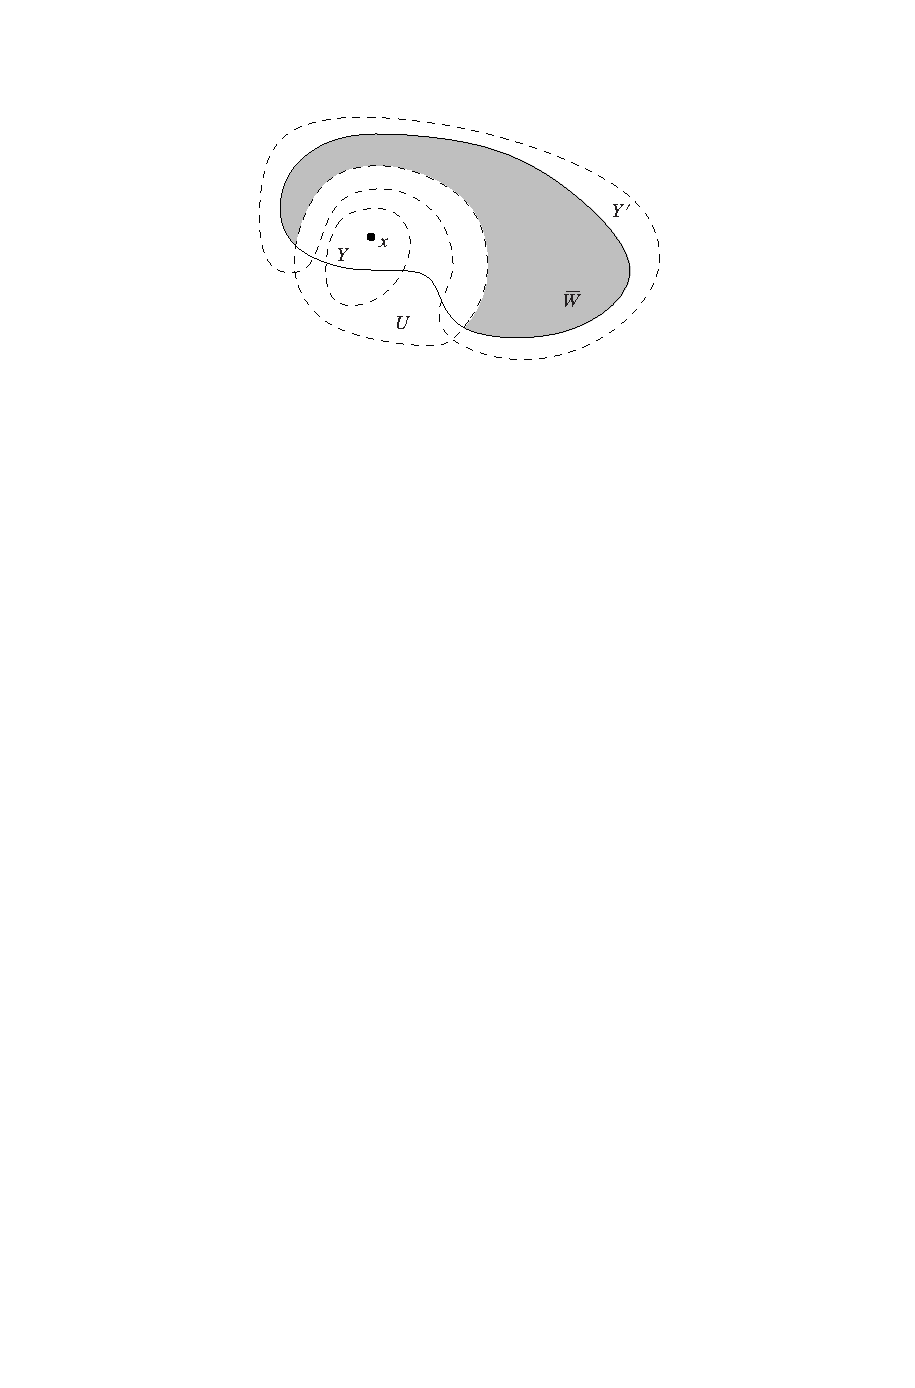
\includegraphics{pictures/local-compact}
\end{figure}
\begin{proof}
Suppose $U$ is a neighborhood of $x$. By Proposition~\ref{Hausdorff local compact iff} there is a precompact neighborhood $W$ of $x$. Then $\widebar{W}\setminus U$ is closed in $\widebar{W}$ and therefore compact. Because compact subsets can be separated by open subsets in a Hausdorff space, there are disjoint open subsets $Y$ containing $x$ and $Y'$ containing $\widebar{W}\setminus U$. Let $V=Y\cap W$. Because $\widebar{V}\sub\widebar{W}$, it is compact.\par
Because $V\sub Y\sub(Y')^c$, we have $\widebar{V}\sub\widebar{(Y')^c}=(Y')^c$. Since $\widebar{W}\setminus U$ is contained in $Y'$, this then implies $\widebar{V}\cap(\widebar{W}\setminus U)=\emp$, and therefore $\widebar{V}\sub\widebar{W}\cap U\sub U$.
\end{proof}
\begin{proposition}\label{LCH precompact nbhd for compact set}
Let $X$ be a locally compact Hausdorff space, let $K$ be a compact subset of $X$, and let $U$ be an neighborhood of $K$. Then there is a precompact neighborhood $V$ of $K$ such that $\widebar{V}\sub U$.
\end{proposition}
\begin{proof}
Lemma~\ref{LCH precompact nbhd closure in nbhd} implies that each point in $K$ has a precompact neighborhood whose closure is included in $U$. Since $K$ is compact, some finite collection of these neighborhoods covers $K$. Let $V$ be the union of the sets in such a finite collection; then $V$ is the required set.
\end{proof}
\begin{proposition}
Any open or closed subset of a locally compact Hausdorff space is a locally compact Hausdorff space.
\end{proposition}
\begin{proof}
Let $X$ be a locally compact Hausdorff space. Note that every subspace of $X$ is Hausdorff, so only local compactness needs to be checked. If $Y\sub X$ is open, Lemma~\ref{LCH precompact nbhd closure in nbhd} says that any point in $Y$ has a neighborhood whose closure is compact and contained in $Y$, so $Y$ is locally compact. Suppose $Z\sub X$ is closed. Any $x\in Z$ has a precompact neighborhood $U$ in $X$. Since $\widebar{U\cap Z}$ is a closed subset of the compact set $\widebar{U}$, it is compact. Since $\widebar{U\cap Z}\sub\widebar{Z}=Z$, it follows that $U\cap Z$ is a precompact neighborhood of $x$ in $Z$. Thus $Z$ is locally compact.
\end{proof}
A subset of a topological space $X$ is a $\bm{G_\delta}$ if it is the intersection of a sequence of open subsets of $X$ and is an $\bm{F_\sigma}$ if it is the union of a sequence of closed subsets of $X$.
\begin{proposition}\label{LCH second countable space G_delta}
Let $X$ be a second countable locally compact Hausdorff space. Then each open subset of $X$ is an $F_\sigma$ and is in fact the union of a sequence of compact sets. Likewise, each closed subset of $X$ is a $G_\delta$.
\end{proposition}
\begin{proof}
Suppose that $\mathcal{U}$ is a countable base for the topology of $X$. Let $U$ be an open subset of $X$, and let $\mathcal{U}_U$ be the collection of those sets $V$ in $\mathcal{U}$ for which $V$ is precompact and included in $U$. Lemma~\ref{LCH precompact nbhd closure in nbhd} implies that $U$ is the union of the closures of the sets in $\mathcal{U}_U$. Thus $U$ is the union of a countable collection of sets that are closed and, in fact, compact.\par
Now suppose that $C$ is a closed subset of $X$. Then $C^c$ is open and so is the union of a sequence $\{F_n\}$ of closed sets. Consequently $C$ is the intersection of the open sets $\{F_n^c\}$.
\end{proof}
Recall that a topological space (or a subset thereof) is $\sigma$-compact if it is the union of a countable collection of compact sets.
\begin{corollary}
Every second countable locally compact Hausdorff space is $\sigma$-compact.
\end{corollary}
\begin{proof}
Since a topological space is an open subset of itself, this is an immediate corollary of Proposition~\ref{LCH second countable space G_delta}.
\end{proof}
\subsection{Continuous functions}
If $X$ is a topological space, the space $\R^X$ of all real-valued functions on $X$ can be topologized in various ways. One way, of course, is the product topology, that is, the topology of pointwise convergence. Another is the \textbf{topology of uniform convergence}, which is generated by the sets
\[\{g\in\R^X:\sup_{x\in X}|g(x)-f(x)|<1/n\}\]
for $f\in\R^X$. Intermediate between these two topologies is the topology of uniform convergence on compact sets, which is generated by the sets
\[\{g\in\R^X:\sup_{x\in K}|g(x)-f(x)|<1/n\}\]
where $f\in\R^X$ and $K\sub X$ is compact. We shall now examine this topology in the case where $X$ is a locally compact Hausdorff space.
\begin{proposition}\label{LCH C(X) closed subspace}
If $X$ is a locally compact Hausdorff space, then $C(X)$ is a closed subspace of $\R^X$ in the topology of uniform convergence on compact sets.
\end{proposition}
\begin{proof}
If $f$ is in the closure of $C(X)$, then $f$ is a uniform limit of continuous functions on each compact $K\sub X$, so $f|_K$ is continuous. If $E\sub\R$ is closed, then $f^{-1}(E)\cap K=(f|_K)^{-1}(E)$ is closed for each compact $K$, so $f^{-1}(E)$ is closed ($X$ is compactly generated), whence $f$ is continuous.
\end{proof}
\begin{proposition}\label{LCH sigma-compact uniform converge on compact iff}
Let $X$ be a $\sigma$-compact locally compact Hausdorff space and $\{K_n\}$ be a exhaustion of $X$ by compact subsets, then for each $f\in\R^X$ the sets
\[\{g\in\R^X:\sup_{x\in K_n}|f(x)-g(x)|<1/m\}\]
form a neighborhood base for $f$ in the topology of uniform convergence on compact sets. Hence this topology is first countable, and $f_n\to f$ uniformly on compact sets if and only if $f_n\to f$ uniformly on each $K_n$.
\end{proposition}
\begin{proof}
These assertions follow easily from the observation that if $K\sub X$ is compact, then $\{\Int K_n\}$ is an open cover of $K$ and hence $K\sub K_n$ for some $n$.
\end{proof}
One may wonder if there are enough continuous functions on a locally compact Hausdorff space. The following results answer this question.
\begin{proposition}[\textbf{Urysohn's Lemma, Locally Compact Version}]\label{LCH Urysohn}
Let $X$ be a locally compact Hausdorff space. If $K$ is a compact subset of $X$ and $U$ is a neighborhood of $K$, then there is a continuous function $f:X\to[0,1]$ such that $f\equiv 1$ on $K$ and $f\equiv 0$ outside a compact subset of $U$.
\end{proposition}
\begin{proof}
By Proposition~\ref{LCH precompact nbhd for compact set}, there exists a precompact neighborhood $V$ of $K$ such that $\widebar{V}\sub U$. Then $V$ is normal, so by Urysohn's lemma there exists a continuous function $f:\widebar{V}\to[0,1]$ such that $f\equiv 1$ on $K$ and $f\equiv 0$ on $\partial V$. We extend $f$ to $X$ by setting $f=0$ on $V$.\par
Now we show that $f$ is a continuous function on $X$. Suppose that $E\sub[0,1]$ is closed. If $0\notin E$, then we have $f^{-1}(E)=(f|_{\widebar{V}})^{-1}(E)$, and if $0\in E$ we have $f^{-1}(E)=(f|_{\widebar{V}})^{-1}(E)\cup(\widebar{V})^c=(f|_{\widebar{V}})^{-1}(E)\cup(V)^c$ (note that $\partial V$ is contained in $(f|_{\widebar{V}})^{-1}(E)$). In either case, $f^{-1}(E)$ is closed, so $f$ is continuous. 
\end{proof}
\begin{proposition}[\textbf{Tietze Extension Theorem, Locally Compact Version}]\label{LCH Tietze Extension}
Let $X$ be a locally compact Hausdorff space and $K$ is a compact subset.
\begin{itemize}
\item[(a)] Any continuous map of $K$ into a closed interval $[a,b]$ may be extended to a continuous map of all of $X$ into $[a,b]$.
\item[(b)] Any continuous map of $K$ into $\R$ may be extended to a continuous map of all of $X$ into $\R$.
\end{itemize}
Moreover, the extension may be taken to vanish outside a compact set.
\end{proposition}
\begin{proof}
We prove (a), and (b) follows as in tietze extension theorem. Let $f:K\to[a,b]$ be a continuous function. Let $V$ be a precompact neighborhood of $K$. Then $\widebar{V}$ is normal, so by Tietze extension theorem there exists a continuous function $F:\widebar{V}\to[a,b]$ such that $F|_K=f$. Since $V$ is a neighborhood of $K$, by \ref{LCH Urysohn} there is a continuous function $\varphi:X\to[0,1]$ such that $\varphi\equiv 1$ on $K$ and $\varphi\equiv 0$ on a compact subset of $V$. Define $\widetilde{F}(x)=F(x)\varphi(x)$. By the choice of $\varphi$, it is easy to see $\widetilde{F}$ is continuous and $\widetilde{F}|_K=f$. Therefore $\widetilde{F}$ is the required function.
\end{proof}
The preceding results show that locally compact Huasdorff spaces have a rich supply of continuous functions that vanish outside compact sets. Let us recall some terminology: If $X$ is a topological space and $f\in C(X)$, the support of $f$, denoted by $\supp(f)$, is the smallest closed set outside of which $f$ vanishes, that is, the closure of $\{x:f(x)\neq 0\}$. If $\supp(f)$ is compact, we say that $f$ is \textbf{compactly supported}, and we define
\[C_c(X)=\{f\in C(X):\text{$\supp(f)$ is compact}\}\]
to be the set of continuous functions on $X$ with compact support. Moreover, if $f\in C(X)$, we say that $f$ \textbf{vanishes at infinity} if for every $\eps>0$ the set $\{x:|f(x)|\geq\eps\}$ is compact, and we define
\[C_0(X)=\{f\in C(X):\text{$f$ vanishes at infinity}\}.\]
Clearly $C_c(X)\sub C_0(X)$. Moreover, $C_0(X)\sub BC(X)$, because for $f\in C_0(X)$ the image of the set $\{x:|f(x)|\geq\eps\}$ is compact, and $|f|<\eps$ on its complement.
\begin{proposition}\label{LCH C_0(X) is closure of C_c(X)}
If $X$ is a locally compact Hausdorff space, then $C_0(X)$ is the closure of $C_c(X)$ in the uniform metric.
\end{proposition}
\begin{proof}
If $\{f_n\}$ is a sequence in $C_c(X)$ that converges uniformly to $f\in C(X)$, for each $\eps>0$ there exists $n\in\N$ such that $\|f-f_n\|<\eps$. Then $|f(x)|<\eps$ for $x\notin\supp(f_n)$, so $f\in C_0(X)$.\par
Conversely, if $f\in C_0(X)$, for $n\in\N$ let $K_n=\{x:|f(x)|\geq 1/n\}$. Then $K_n$ is compact, so by Proposition~\ref{LCH Urysohn} there exists $\varphi_n\in C_c(X)$ with $0\leq\varphi_n\leq 1$ and $\varphi_n\equiv 1$ on $K_n$. Let $f_n=\varphi_nf$. Then $f_n\in C_c(X)$ and $\|f_n-f\|_{\infty}\leq 1/n$, so $f_n$ converges to $f$ uniformly.
\end{proof}
Now we derive some consequences of Proposition~\ref{LCH Urysohn} which will be used later. Let us begin with the following lemma.
\begin{lemma}\label{compact set separated by open union}
Let $X$ be a Hausdorff space, let $K$ be a compact subset of $X$, and let $U_1$ and $U_2$ be open subsets of $X$ such that $K\sub U_1\cup U_2$. Then there are compact sets $K_1$ and $K_2$ such that $K=K_1\cup K_2$, $K_1\sub U_1$ and $K_2\sub U_2$.
\end{lemma}
\begin{proof}
Let $L_1=K\setminus U_1$ and $L_2=K\setminus U_2$. Then $L_1$ and $L_2$ are disjoint and compact, and so according to Lemma~\ref{topological space compact separated by disjoint open} they can be separated by disjoint open sets, say by $V_1$ and $V_2$. If we define $K_1$ and $K_2$ by $K_1=K\setminus V_1$ and $K_2=K\setminus V_2$, then $K_1$ and $K_2$ are compact, are included in $U_1$ and $U_2$, respectively, and have $K$ as their union.
\end{proof}
\begin{proposition}\label{LCH decompose function with supp in open set}
Let $X$ be a locally compact Hausdorff space, let $f$ belong to $C_c(X)$, and let $U_1,\dots,U_n$ be open subsets of X such that $\supp(f)\sub U=\bigcup_{i=1}^{n}U_i$. Then there are functions $f_1,\dots,f_n$ in $C_c(X)$ such that $f=f_1+\cdots+f_n$ and such that for each $i$ the support of $f_i$ is contained in $U_i$. Furthermore, if the function $f$ is nonnegative, then the functions $f_1,\dots,f_n$ can be chosen so that all are nonnegative.
\end{proposition}
\begin{proof}
In case $n=1$ we need only let $f_1$ be $f$. So we can begin by supposing that $n=2$. Use Lemma~\ref{compact set separated by open union} to construct compact sets $K_1$ and $K_2$ such that $K_1\sub U_1$ and $K_2\sub U_2$, and $\supp(f)=K_1\cup K_2$, and then use Proposition~\ref{LCH Urysohn} to construct functions $h_1$ and $h_2$ that belong to $C_c(X)$ and satisfy $\chi_{K_i}\leq h_i\leq\chi_{U_i}$ and $\supp(h_i)\sub U_i$ for $i=1,2$. Define functions $g_1$ and $g_2$ by $g_1=h_1$ and $g_2=h_2-(h_1\wedge h_2)$. Then $g_1$ and $g_2$ are non-negative, their supports are included in $U_1$ and $U_2$, respectively, and they satisfy
\[g_1+g_2=h_1+h_2-(h_1\wedge h_2)=h_1\vee h_2=1.\]
at each $x$ in $\supp(f)$. We can complete the proof in the case where $n=2$ by defining $f_1$ and $f_2$ to be $fg_1$ and $fg_2$, and the general case follows by induction.
\end{proof}
\begin{proposition}\label{LCH function fixed finite value}
Let $X$ be a locally compact Hausdorff space, let $K_1,\dots,K_n$ be disjoint compact subsets of $X$, and let $\alpha_1,\dots,\alpha_n$ be real (or complex) numbers. Then there is a function $f$ that belongs to $C_c(X)$ and satisfies
\begin{itemize}
\item[(a)] $f(x)=\alpha_i$ if $x\in K_i$, for $i=1,\dots,n$.
\item[(b)] $\|f\|_{\infty}=\max\{|a_1|,\dots,|a_n|\}$.
\end{itemize}
\end{proposition}
\begin{proof}
We begin by constructing disjoint open sets $U_1,\dots,U_n$ such that $K_i\sub U_i$ holds for each $i$. If $n=2$, such sets are provided by Lemma~\ref{topological space compact separated by disjoint open}. The general case follows by induction. Next we use Proposition~\ref{LCH Urysohn} to choose functions $f_1,\dots,f_n$ that belong to $C_c(X)$ and satisfy $\chi_{K_i}\leq f_i\leq\chi_{U_i}$ for $i=1,\dots,n$. The required function $f$ is now given by $f=\sum_{i=1}^{n}\alpha_if_i$.
\end{proof}
\subsection{One-point compactification}
If $X$ is a noncompact locally compact Hausdorff space, it is possible to make $X$ into a compact space by adding a single point "at infinity" in such a way that the functions in $C_0(X)$ are precisely those continuous functions $f$ such that $f(x)\to 0$ as $x$ approaches the point at infinity. Here is the precise definition of this space.
\begin{proposition}\label{one point compactification}
Let $X$ be a topological space. Then $X$ is locally compact Hausdorff if and only if there exists a space $X^*$ satisfying the following conditions:
\begin{itemize}
\item[(a)] $X$ is a subspace of $X^*$.
\item[(b)] $X^*\setminus X$ consists of a single point.
\item[(c)] $X^*$ is a compact Huasdorff space.
\end{itemize}
If $X_1$ and $X_2$ are two spaces satisfying these conditions, then there is a homeomorphism of $X_1$ with $X_2$ that equals the identity map on $X$.
\end{proposition}
\begin{proof}
We first verify uniqueness. Let $X_1$ and $X_2$ be two spaces satisfying these conditions. Define $h:X_1\to X_2$ by letting $h$ map the single point $p$ of $X_1\setminus X$ to the point $q$ of $X_2\setminus X$, and letting $h$ equal the identity on $X$. We show that if $U$ is open in $X_2$, then $h(U)$ is open in $X_2$. Symmetry then implies that $h$ is a homeomorphism.\par
First, consider the case where $U$ does not contain $p$. Then $h(U)=U$. Since $U$ is open in $X_1$ and is contained in $X$, it is open in $X$. Because $X$ is open in $X_2$, the set $U$ is also open in $X_2$, as desired. Second, suppose that $U$ contains $p$. Since $C=X_1\setminus U$ is closed in $X_1$, it is compact as a subspace of $X_1$. Because $C$ is contained in $X$, it is a compact subspace of $X$. Then because $X$ is a subspace of $X_2$, the space $C$ is also a compact subspace of $X_2$, and hence is closed in $X_2$. So $h(U)=X_2\setminus C$ is open, as desired.\par
Now we suppose $X$ is locally compact Hausdorff and construct the space $X^*$. Let us take some object that is not a point of $X$, denote it by the symbol $\infty$ for convenience, and adjoin it to $X$, forming the set $X^*=X\cup\{\infty\}$. Topologize $X^*$ by defining the collection of open sets of $X^*$ to consist of $(1)$ all sets $U$ that are open in $X$, and $(2)$ all sets of the form $X^*\setminus C$, where $C$ is a compact subspace of $X$. We need to check that this collection is in fact a topology on $X^*$. The empty set is a set of type $(1)$, and the space $X^*$ is a set of type $(2)$. Checking that the intersection of two open sets is open involves two cases:
\[(X^*\setminus C_1)\cap(X^*\setminus C_2)=X^*\setminus(C_1\cup C_2),\quad U_1\cap(X^*\setminus C_1)=U_1\cap(X\setminus C_1).\]
Similarly, checking that arbitrary union open sets is open involves two cases:
\[\bigcup_\alpha(X^*\setminus C_\alpha)=X^*\setminus\bigcap_\alpha C_\alpha,\quad\Big(\bigcup_\alpha U_\alpha\Big)\cup\bigcup_\beta(X^*\setminus C_\beta)=U\cup(X^*\setminus C)=X^*\setminus(C\setminus U).\]
Therefore we have defined a topology on $X^*$.\par
Now we show that $X$ is a subspace of $X^*$. Given any open set of $X^*$, we show its intersection with $X$ is open in $X$. If $U$ is of type $(1)$, then $U\cap X=U$; if $U=X^*\setminus C$ is of type $(2)$, then $U\cap X=X\setminus C$; both of these sets are open in $X$. Conversely, any set open in $X$ is a set of type $(1)$ and therefore open in $X^*$ by definition.\par
To show that $X^*$ is compact, let $\mathcal{U}$ be an open covering of $X^*$. The collection $\mathcal{U}$ must contain an open set of type $(2)$, say $X^*\setminus C$, since none of the open sets of type $(1)$ contain the point $\infty$. Take all the members of $\mathcal{U}$ different from $X^*\setminus C$ and intersect them with $X$; they form a collection of open sets of $X$ covering $C$. Because $C$ is compact, finitely many of them  over $C$; the corresponding finite collection of elements of $\mathcal{U}$ will, along with the element $X^*\setminus C$, cover all of $X^*$. Therefore $X^*$ is compact.\par
To show that $X^*$ is Hausdorff, let $x$ and $y$ be two distinct points of $X^*$. If both of them lie in $X$, there are disjoint sets $U$ and $V$ open in $X$ containing them, respectively, since $X$ is Huasdorff. On the other hand, if $x\in X$ and $y=\infty$, we can choose a compact set $C$ in $X$ containing a neighborhood $U$ of $x$. Then $U$ and $X^*\setminus C$ are disjoint neighborhoods of $x$ and $\infty$, respectively, in $X^*$.\par
Finally, we prove the converse. Suppose a space $X^*$ satisfying conditions (a)---(c) exists. Then $X$ is Hausdorff because it is a subspace of the Hausdorff space $X^*$. Given $x\in X$, we show $X$ is locally compact at $x$. Choose disjoint open sets $U$ and $V$ of $X^*$ containing $x$ and the single point of $X^*\setminus X$, respectively. Then the set $C=X^*\setminus V$ is closed in $X^*$, so it is a compact subspace of $X^*$. Since $C$ lies in $X$, it is also compact as a subspace of $X$; it contains the neighborhood $U$ of $x$.
\end{proof}
If $X$ itself should happen to be compact, then the space $X^*$ of the preceding theorem is not very interesting, for it is obtained from $X$ by adjoining a single isolated point. However, if $X$ is not compact, then the point of $X^*\setminus X$ is a limit point of $X$, so that $\widebar{X}=X^*$.
\begin{definition}
If $Y$ is a compact Hausdorff space and $X$ is a proper subspace of $Y$ whose closure equals $Y$, then $Y$ is said to be a compactification of $X$. If $Y\setminus X$ equals a single point, then $Y$ is called the \textbf{one-point compactification} of $X$.
\end{definition}
\begin{example}
The one-point compactification of the real line $\R$ is homeomorphic with
the circle, as you may readily check. Similarly, the one-point compactification of $\R^2$ is homeomorphic to the sphere $S^2$. If $\R^2$ is looked at as the space $\C$ of complex numbers, then $\C\cup\{\infty\}$ is called the \textbf{Riemann sphere}, or the \textbf{extended complex plane}.
\end{example}
\begin{proposition}\label{LCH one-point compactification continuous function}
Let $X$ be a locally compact Hausdorff space and $X^*$ be its one-point compactification. Let $f\in C(X)$, then $f$ extends continuously to $X^*$ if and only if $f$ has a limit at the point infinity. That is, if and only if $f=g+a$ where $g\in C_0(X)$ and $a$ is a constant, in which case the continuous extension is given by $f(\infty)=a$.
\end{proposition}
\begin{proof}
Let $f$ be the form stated above. We extend $f$ to $X^*$ by defining $f(\infty)=a$. We only need to check that $f$ is continuous at $\infty$, since $f$ is in $C(X)$ and every open set of $X$ is open in $X^*$. Let $\eps>0$ be arbitrary, then the set $C_\eps=\{x:|g(x)|\geq\eps\}$ is compact in $X$, and hence $X^*\setminus C_\eps$ is a neighborhood of $\infty$ in $X^*$. By definition, this then implies $|f(x)-a|<\eps$ for $x\in X^*\setminus C_\eps$. Therefore $f$ is continuous at $\infty$, and so $f\in C(X^*)$.\par
Conversely, assume that $f\in C(X)$ has an extension $\widetilde{f}$ on $X^*$. Define $a=\widetilde{f}(\infty)$ and $g(x)=f(x)-a$. We need to show that $g\in C_0(X)$. Let $\eps>0$, then there exists a neighborhood $U$ of $\infty$ in $X^*$ such that $f(U)\sub(a-\eps,a+\eps)$. By the topology of $X^*$, since $\infty\in U$, $X\setminus U$ is then compact in $X$. Since $\{x:|g(x)|\geq\eps\}=\{x:|f(x)-a|\geq\eps\}$ is contained in $X\setminus U$, it is also compact, as desired.
\end{proof}
\subsection{Stone-Weierstrass theorem}
In this part we prove a far-reaching generalization of the well-known theorem of Weierstrass to the effect that any continuous function on a compact interval $[a,b]$ is the uniform limit of polynomials on $[a,b]$. In what follows, $X$ will denote a compact Hausdorff space, and we equip the space $C(X)$ with the uniform metric.\par
A subset $\mathscr{A}$ of $C(X,\R)$ or $C(X,\C)$ is said to be \textbf{separating} if for every $x,y\in X$ with $x\neq y$ there exists $f\in\mathscr{A}$ such that $f(x)\neq f(y)$. $\mathscr{A}$ is called an \textbf{algebra} if it is a real (resp. complex) vector subspace of $C(X,\R)$ (resp. $C(X,\C)$) such that $fg\in\mathscr{A}$ whenever $f,g\in\mathscr{A}$. If $\mathscr{A}\sub C(X,\R)$, $\mathscr{A}$ is called a \textbf{lattice} if $\max(f,g)$ and $\min(f,g)$ are in $\mathscr{A}$ whenever $f,g\in\mathscr{A}$. Since the algebra and lattice operations are continuous, one easily sees that if $\mathscr{A}$ is an algebra or a lattice, so is its closure $\mathscr{A}$ in the uniform metric.
\begin{theorem}[\textbf{Stone-Weierstrass Theorem}]\label{Stone-Weierstrass}
Let $X$ be a compact Hausdorff space. If $\mathscr{A}$ is a separating closed subalgebra of $C(X,\R)$, then either $A=C(X,\R)$ or $A=\{f\in C(X,\R):f(x_0)=0\}$ for some $x_0\in X$. The first alternative holds iff $\mathscr{A}$ contains the constant functions.
\end{theorem}
The proof will require several lemmas. The first one, in effect, proves the theorem when $X$ consists of two points, and the second one is a special case of the classical Weierstrass theorem for $X=[-1,1]$. After these two we return to the general case.
\begin{lemma}\label{Stone-Weierstrass subalgebra of R^2}
Consider $\R^2$ as an algebra under coordinatewise addition and multiplication. Then the only subalgebras of $\R^2$ are $\R^2$, $\{(0,0)\}$, and the linear span of $(1,0)$, $(0,1)$, or $(1,1)$.
\end{lemma}
\begin{proof}
The subspaces of $\R^2$ listed above are evidently subalgebras. If $\mathscr{A}\sub\R^2$ is a nonzero algebra and $(0,0)\neq(a,b)\in\mathscr{A}$, then $(a^2,b^2)\in\mathscr{A}$. If $a,b$ are nonzero and distinct then $(a,b)$ and $(a^2,b^2)$ are linearly independent, so $A=\R^2$. The other possibilities give the other three subalgebras.
\end{proof}
\begin{lemma}\label{Stone-Weierstrass approximate |x|}
For any $\eps>0$ there is a polynomial $P$ on $\R$ such that $P(0)=0$ and $||x|-P(x)|<\eps$ for $x\in[-1,1]$.
\end{lemma}
\begin{proof}
Consider the Maclaurin series for $(1-t)^{1/2}$:
\[(1-t)^{1/2}=1-\sum_nc_nt^n.\]
By the ratio test, this series converges for $|t|<1$. Moreover, by the monotone convergence theorem (applied to counting measure on $\N$),
\[\sum_nc_n=\lim_{t\to 1^-}\sum_nc_nt^n=1-\lim_{t\to 1-}(1-t)^{1/2}=1.\]
It follows from the finiteness of $\sum_nc_n$ that the series $1-\sum_nc_nt^n$ converges absolutely and uniformly on $[-1,1]$, and its sum is $(1-t)^{1/2}$ there. Therefore, given $\eps>0$, by taking a suitable partial sum of this series we obtain a polynomial $Q$ such that $|(1-t)^{1/2}-Q(t)|<\eps/2$ for $t\in[-1,1]$. Set $t=1-x^2$ and $R(x)=Q(1-x^2)$, we obtain a polynomial $R$ such that $||x|-R(x)|<\eps/2$ for $x\in[-1,1]$. In particular, $|R(0)|<\eps/2$. If we set $P(x)-R(x)-R(0)$, we then get the claim. 
\end{proof}
\begin{lemma}\label{Stone-Weierstrass closed subalgebra is lattice}
If $\mathscr{A}$ is a closed subalgebra of $C(X,\R)$, then $|f|\in\mathscr{A}$ whenever $f\in\mathscr{A}$; hence $\mathscr{A}$ is a lattice.
\end{lemma}
\begin{proof}
If $f\in\mathscr{A}$ and $f\neq 0$, let $h=f/\|f\|_\infty$. Then $h$ maps $X$ into $[-1,1]$, so if $\eps>0$ and $P$ is as in Lemma~\ref{Stone-Weierstrass approximate |x|}, we have $||h|-P\circ h|<\eps$. Since $P(0)=0$, $P$ has no constant term, so $P\circ h\in\mathscr{A}$ since $\mathscr{A}$ is an algebra. Since $\mathscr{A}$ is closed and $\eps$ is arbitrary, we have $|h|\in\mathscr{A}$ and hence $|f|\in\mathscr{A}$. This proves the first assertion, and the second one follows because $\max(f,g)$ and $\min(f,g)$ can be represented by $f$, $g$, and $|f-g|$.
\end{proof}
\begin{lemma}\label{Stone-Weierstrass two point}
Suppose $\mathscr{A}$ is a closed lattice in $C(X,\R)$ and $f\in C(X,\R)$. If for every $x,y\in X$ there exists $h_{xy}\in\mathscr{A}$ such that $h_{xy}(x)=f(x)$ and $h_{xy}(y)=f(y)$, then $f\in\mathscr{A}$.
\end{lemma}
\begin{proof}
Given $\eps>0$, for each $x,y\in X$ let
\[U_{xy}=\{z\in X:f(z)<h_{xy}(z)+\eps\},\quad V_{xy}=\{z\in X:f(z)>h_{xy}(z)-\eps\}.\]
These sets are open and contain $x$ and $y$. Fix $y$, then $\{U_{xy}:x\in X\}$ covers $X$, so there is a finite subcover $\{U_{x_jy}\}$. Let $h_y=\max(h_{x_1y},\dots,h_{x_ny})$, then $f<h_y+\eps$ on $X$ and $f>h_y-\eps$ on $V_y=\bigcup_{i=1}^{n}V_{x_iy}$, which is open and contains $y$. Thus $\{V_y:y\in X\}$ is another open cover of $X$, so there is a finite subcover $\{V_{y_j}\}$. Let $h=\min(h_{y_1},\dots,h_{y_m})$, then $\|f-h\|<\eps$. Since $\mathscr{A}$ is a lattice, $h\in\mathscr{A}$, and since $\mathscr{A}$ is closed and $\eps$ is arbitrary, $f\in\mathscr{A}$.
\end{proof}
\begin{proof}[Proof of Theorem~\ref{Stone-Weierstrass}]
Given $x\neq y\in X$, let $\mathscr{A}_{xy}=\{(f(x),f(y)):f\in\mathscr{A}\}$. Then $\mathscr{A}_{xy}$ is a subalgebra of $\R^2$ as in Lemma~\ref{Stone-Weierstrass subalgebra of R^2} because $f\mapsto(f(x),f(y))$ is an algebra homomorphism. If $\mathscr{A}_{x,y}=\R^2$ for all $x,y$, then Lemmas~\ref{Stone-Weierstrass closed subalgebra is lattice} and \ref{Stone-Weierstrass two point} imply that $\mathscr{A}=C(X,\R)$. Otherwise, there exist $x,y$ for which $\mathscr{A}_{xy}$ is a proper subalgebra of $\R^2$. It cannot be $\{(0,0)\}$ or the linear span of $(1,1)$ because $\mathscr{A}$ separates points, so by Lemma~\ref{Stone-Weierstrass subalgebra of R^2} $\mathscr{A}_{xy}$ is the linear span of $(1,0)$ or $(0,1)$. In either case there exists $x_0\in X$ such that $f(x_0)=0$ for all $f\in\mathscr{A}$. There is only one such $x_0$ since $A$ separates points, so if neither $x$ nor $y$ is $x_0$, we have $\mathscr{A}_{xy}=\R^2$. Lemmas~\ref{Stone-Weierstrass closed subalgebra is lattice} and \ref{Stone-Weierstrass two point} now imply that $\mathscr{A}=\{f\in C(X,\R):f(x_0)=0\}$. Finally, if $\mathscr{A}$ contains constant functions, there is no $x_0$ such that $f(x_0)=0$ for all $f\in\mathscr{A}$, so $\mathscr{A}$ must equal $C(X,\R)$.
\end{proof}
We have stated the Stone-Weierstrass theorem in the form that is most natural for the proof. However, in applications one is typically dealing with a subalgebra $\mathscr{B}$ of $C(X,\R)$ that is not closed, and one applies the theorem to $\mathscr{A}=\widebar{\mathscr{B}}$. The resulting
restatement of the theorem is as follows:
\begin{corollary}
Suppose $\mathscr{B}$ is a separating subalgebra of $C(X,\R)$. If there exists $x_0\in X$ such that $f(x_0)=0$ for all $f\in\mathscr{B}$, then $\mathscr{B}$ is dense in $\{f\in C(X,\R):f(x_0)=0\}$. Otherwise, $\mathscr{B}$ is dense in $C(X,\R)$.
\end{corollary}
The classical Weierstrass approximation theorem is the special case where $X$ is a compact subset of $\R^n$ and $\mathscr{B}$ is the algebra of polynomials on $\R^n$ (restricted to $X$); here $\mathscr{B}$ contains the constant functions, so the conclusion is that it is dense in $C(X,\R)$.\par
The Stone-Weierstrass theorem, as it stands, is false for complex-valued functions. For example, the algebra of polynomials in one complex variable is not dense in $C(K)$ for most compact subsets $K$ of $\C$. (In particular, if $\Int K\neq\emp$, any uniform limit of polynomials on $K$ must be holomorphic on $\Int K$.) Here we shall give a simple proof that the function $f(z)=\bar{z}$ cannot be approximated uniformly by polynomials on the unit circle. If $P(z)=\sum_ja_jz^j$, then
\[\int_{0}^{2\pi}\widebar{f(e^{it})}P(e^{it})\,dt=\sum_{j=0}^{n}a_j\int_0^{2\pi}e^{i(j+1)t}\,dt=0.\]
Since $|f|=1$ on the unit circle we have
\[2\pi=\int_0^{2\pi}\bar{f}f\,dt\Big|\leq\Big|\int_0^{2\pi}\bar{f}(f-P)\,dt\Big|+\Big|\int_0^{2\pi}\bar{f}P\,dt\Big|\leq\int_0^{2\pi}|f-P|\,dt\leq 2\pi\|f-P\|_\infty.\]
Therefore, $\|f-P\|_\infty\geq 1$ for any polynomial $P$.\par
There is, however, a complex version of the Stone-Weierstrass theorem.
\begin{theorem}[\textbf{Complex Stone-Weierstrass Theorem}]\label{Stone-Weierstrass complex}
Let $X$ be a compact Hausdorff space. If $\mathscr{A}$ is a separating closed complex subalgebra of $C(X,\C)$ that separates points and is closed under complex conjugation, then either $A=C(X,\C)$ or $A=\{f\in C(X,\C):f(x_0)=0\}$ for some $x_0\in X$.
\end{theorem}
\begin{proof}
Since $\Re(f)=(f+\bar{f})/2$ and $\Im(f)=(f-\bar{f})/2i$, the set $\mathscr{A}_{\R}$ of real and imaginary parts of functions in $\mathscr{A}$ is a subalgebra of $C(X,\R)$ to which the Stone-Weierstrass theorem applies. Since $\mathscr{A}=\mathscr{A}_{\R}+i\mathscr{A}_{\R}$, the desired result follows.
\end{proof}
There is also a version of the Stone-Weierstrass theorem for locally compact Hausdorff spaces.
\begin{theorem}
Let $X$ be a locally compact Hausdorff space. If $\mathscr{A}$ is a separating closed subalgebra of $C_0(X,\R)$, then either $\mathscr{A}=C_0(X,\R)$ or $\mathscr{A}=\{f\in C_0(X,\R):f(x_0)=0\}$ for some $x_0\in X$.
\end{theorem}
\begin{proof}
If there exists $x_0\in X$ such that $f(x_0)=0$ for all $f\in\mathscr{A}$, let $Y$ be the one-point compactification of $X\setminus\{x_0\}$. Then by Proposition~\ref{LCH one-point compactification continuous function} we can write $\mathscr{A}\sub\{f\in C(Y,\R):f(+\infty)=0\}$. Since $\mathscr{A}$ separates points on $X\setminus\{x_0\}$, there is no $y\in X\setminus\{x_0\}$ such that $f(y)=0$ for all $f\in\mathscr{A}$; it follows that $\mathscr{A}$ separates points in $Y$, and by the Stone-Weierstrass theorem we get $\mathscr{A}=\{f\in C(Y,\R):f(+\infty)=0\}=\{f\in C_0(X,\R):f(x_0)=0\}$.\par
If there is no $x_0\in X$ such that $f(x_0)=0$ for all $f\in\mathscr{A}$, let $Y$ be the one-point compactification of $X$. By the same proof we see $\mathscr{A}=C_0(X,\R)$.
\end{proof}
By the same proof as Theorem~\ref{Stone-Weierstrass complex}, we also have the following complex version.
\begin{theorem}
Let $X$ be a locally compact Hausdorff space. If $\mathscr{A}$ is a separating closed complex subalgebra of $C_0(X,\C)$ that separates points and is closed under complex conjugation, then either $A=C(X,\C)$ or $A=\{f\in C(X,\C):f(x_0)=0\}$ for some $x_0\in X$.
\end{theorem}
\subsection{Metrizability}
Now we consider metrizability of locally compact spaces.
\begin{proposition}\label{compact Hausdorff metrizable iff C_2}
A compact Hausdorff space is metrizable if and only if it is second countable.
\end{proposition}
\begin{proof}
First suppose that $X$ is compact and metrizable. Then $X$ is separable and so is second countable.\par
Now suppose that $X$ is a compact Hausdorff space that is second countable and let $\mathcal{U}$ be a countable base. The space $X$ is normal, and so for each pair of sets $U$, $V$ that belong to $\mathcal{U}$ and satisfy $U\cap V=\emp$ there is, by Urysohn's lemma, a continuous function $f:X\to[0,1]$ that vanishes on $\widebar{U}$ and has value $1$ everywhere on $\widebar{V}$. Form a sequence $\{f_n\}$ by choosing one such function for each such pair of sets. Our next step is to check that this sequence of functions separates the points of $X$, and for this it is enough to show that for each pair $x$, $y$ of distinct points in $X$ there are sets $U$ and $V$ that belong to $\mathcal{U}$, have disjoint closures, and contain $x$ and $y$, respectively. To construct such sets, choose disjoint open neighborhoods $W_1$ and $W_2$ of $x$ and $y$, and use Lemma~\ref{LCH precompact nbhd closure in nbhd} to choose open sets $U$ and $V$ such that $x\in U\sub\widebar{U}\sub W_1$ and $y\in V\sub\widebar{V}\sub W_2$. By making $U$ and $V$ a bit smaller, if necessary, we can assume that they belong to $\mathcal{U}$. Thus the required sets $U$ and $V$ exist, and the sequence $\{f_n\}$ separates the points of $X$.\par
Define a function $d:X\times X\to\R$ by setting
\[d(x,y)=\sum_{n=1}^{\infty}\frac{1}{2^n}|f_n(x)-f_n(y)|.\]
It is easy to use the fact that the functions $\{f_n\}$ separate the points of $X$ to check that $d$ is a metric on the set $X$ and to use the fact that the functions $\{f_n\}$ are continuous (with respect to the original topology on $X$) to check that the topology induced by $d$ is weaker than the original topology. Since the original topology makes $X$ a compact space, while the topology induced by $d$ is weaker and Hausdorff, the two topologies must be the same ($\id$ is a continuous bijection from a compact space to a Huasdorff space). Thus the original topology on $X$ is metrizable and in fact is metrized by $d$.
\end{proof}
Our next task is to prove that each second countable locally compact Hausdorff space is metrizable. For this we need the following lemma.
\begin{lemma}\label{LCH C_2 iff onepoint compactification C_2}
Let $X$ be a locally compact Hausdorff space. If $X$ is second countable, then the one-point compactification of $X$ is also second countable.
\end{lemma}
\begin{proof}
Let $\mathcal{U}$ be a countable base for the topology of $X$, and let $\mathcal{U}_0$ be the collection of those sets $V$ in $\mathcal{U}$ for which $V$ is precompact. Arrange the sets in $\mathcal{U}_0$ in a sequence, say $\{V_k\}$. Then $X=\bigcup_kV_k$, since $X$ is locally compact, and so for each compact subset $K$ of $X$ there is a positive integer $n$ such that $K\sub\bigcup_{k=1}^{n}V_k$. Thus if $U$ is an open neighborhood in $X^*$ of the point at infinity and if $K=X^*\setminus U$, then there is a positive integer $n$ such that $K\sub\bigcup_{k=1}^{n}V_k$ and hence such that $X^*\setminus\widebar{\bigcup_{k=1}^{n}V_k}\sub U$. It follows that the sets in $U$, together with the sets $X^*\setminus\widebar{\bigcup_{k=1}^{n}V_k}$, form a countable base for the topology of $X^∗$.
\end{proof}
\begin{proposition}\label{LCH C_2 is metrizable}
Each secound countable locally compact Hausdorff space is metrizable.
\end{proposition}
\begin{proof}
Let $X$ be a secound countable locally compact Hausdorff space. Proposition~\ref{compact Hausdorff metrizable iff C_2} and Lemma~\ref{LCH C_2 iff onepoint compactification C_2} imply that the one-point compactification $X^*$ of $X$ is metrizable. Then $X$, as a subspace of the metrizable space $X^*$, is metrizable.
\end{proof}
\section{Proper maps}
\subsection{Proper maps}
If $f$ and $g$ are closed continuous maps, it does not follow that $f\times g$ is closed, even if $f$ is the identity map. An example is given below.
\begin{example}
Every constant mapping into a Hausdorff space is closed. But it $f$ is the constant mapping $\Q\to\{0\}$, then $f\times\id_\Q$ is the mapping $(x,y)\mapsto(0,y)$ of $\Q^2$ into $\Q^2$, so it is the second projection and is not closed.
\end{example}
\begin{definition}
A map $f:X\to Y$ is said to be \textbf{proper} if $f$ is continuous and if the mapping $f\times\id_Z:X\times Z\to Y\times Z$ is closed, for every topological space $Z$.
\end{definition}
If in the definition we take the space $Z$ to consist of a single point, then we see that any proper map is closed. A partial converse holds when the map $f$ is injective:
\begin{proposition}\label{topological space injection proper iff}
Let $f:X\to Y$ be a continuous injection. Then the following three statements are equivalent.
\begin{itemize}
\item[(\rmnum{1})] $f$ is proper.
\item[(\rmnum{2})] $f$ is closed.
\item[(\rmnum{3})] $f$ is a homeomorphism of $X$ onto a closed subset of $Y$.
\end{itemize}
\end{proposition}
\begin{proof}
We have just seen that (\rmnum{1}) implies (\rmnum{2}). Since the equivalence relation $f(x)=f(y)$ is the equality relation, the quotient space of $X$ with respect to this relation can be identified with $X$; hence (\rmnum{2}) implies (\rmnum{3}) by Proposition~\ref{topological space canonical decomposition homeomorphism iff}. Finally, if (\rmnum{3}) is satisfied then $f\times\id_Z$ is a homeomorphism of $X\times Z$ onto a closed subspace of $Y\times Z$ and is therefore a closed mapping; hence (\rmnum{3}) implies (\rmnum{1}).
\end{proof}
\begin{proposition}\label{topological space proper map on subspace}
Let $f:X\to Y$ be a continuous map. If $B$ is any subset of $Y$, let $f_B$ denote the restriction of $f$ on $f^{-1}(B)$.
\begin{itemize}
\item[(a)] If $f$ is proper, so is $f_B$.
\item[(b)] Let $(B_i)_{i\in I}$ be a family of subsets of $Y$ whose interiors cover $Y$, or which is a locally finite closed covering of $Y$; then if each of the mappings $f_B$ is proper, so is $f$.
\end{itemize}
\end{proposition}
\begin{proof}
Let $Z$ be a topological space. If $B$ is any subset of $Y$, we have
\[f_B\times\id_Z=(f\times\id_Z)_{B\times Z}.\]
If $f$ is proper, then $f\times\id_Z$ is closed, hence so is $(f\times\id_Z)_{B\times Z}$ (Proposition~\ref{}), whence (a) is proved. If now $(B_i)_{i\in I}$ satisfies one of the two conditions stated in (b), then the covering $(B_i\times Z)_{i\in I}$ of $Y\times Z$ has the same property; if the $f_{B_i}$ are proper then the mappings $(f\times\id_Z)_{B\times Z}$ are closed, whence $f\times\id_Z$ is closed (Proposition~\ref{}). This completes the proof.
\end{proof}
\begin{proposition}
Let $f:X\to Y$ and $g:Y\to Z$ be two continuous mappings.
\begin{itemize}
\item[(a)] If $f$ and $g$ are proper, then $g\circ f$ is proper.
\item[(b)] If $g\circ f$ is proper and $f$ is surjective, then $g$ is proper.
\item[(c)] If $g\circ f$ is proper and $g$ is injective, then $f$ is proper. 
\item[(d)] If $g\circ f$ is proper and $Y$ is Hausdorff, then $f$ is proper   
\end{itemize}
\end{proposition}
\begin{proof}

\end{proof}
\subsection{Proper maps}
If $X$ and $Y$ are topological spaces, a map $f:X\to Y$ (continuous or not) is said to be \textbf{proper} if the preimage of each compact subset of $Y$ is compact. For example, every exhaustion function $f:X\to\R$ is a proper map.\par
In order to visualize the behavior of proper maps, it is useful to introduce the following definition: if $X$ is a topological space, a sequence $(x_i)$ in $X$ is said to \textbf{diverge to infinity} if for every compact set $K\sub X$ there are at most finitely many values of $i$ for which $x_i\in K$.
\begin{lemma}\label{topological space diverge to inf iff no convergent subseq}
Suppose $X$ is a first countable Hausdorff space. A sequence in $X$ diverges to infinity if and only if it has no convergent subsequence.
\end{lemma}
\begin{proof}
Assume first that $(x_i)$ is a sequence in $X$ that diverges to infinity. If there is a subsequence $(x_{i_j})$ that converges to $x\in X$, then the set $K=\{x\}\cup\{x_{i_j}\}$ is compact and contains infinitely many terms of the sequence, which is a contradiction. (This implication does not require the hypothesis that $X$ is first countable and Hausdorff.)\par
Conversely, assume that $(x_i)$ has no convergent subsequence. If $K\sub X$ is any compact set that contains $x_i$ for infinitely many $i$ , then there is a subsequence $(x_{i_j})$ such that $x_{i_j}\in K$ for all $j$. Because a compact, first countable Hausdorff space is sequentially compact, this subsequence in turn has a convergent subsequence, which is a contradiction.
\end{proof}
\begin{proposition}
Suppose $X$ and $Y$ are topological spaces and $f:X\to Y$ is a proper map. Then $f$ takes every sequence diverging to infinity in $X$ to a sequence diverging to infinity in $Y$.
\end{proposition}
\begin{proof}
Suppose $(x_i)$ is a sequence in $X$ that diverges to infinity. If $\big(f(x_i)\big)$ does not diverge to infinity, then there is a compact subset $K\sub Y$ that contains $f(x_i)$ for infinitely many values of $i$. It follows that $x_i$ lies in the compact set $f^{-1}(K)$ for these values of $i$, which contradicts the assumption that $(x_i)$ diverges to infinity.
\end{proof}
Because the definition of properness is sometimes tricky to check directly, it is useful to have other sufficient conditions for a map to be proper. The next proposition gives several such conditions.
\begin{proposition}\label{proper map if}
Suppose $X$ and $Y$ are topological spaces, and $f:X\to Y$ is a continuous map.
\begin{itemize}
\item[(a)] If $X$ is compact and $Y$ is Hausdorff, then $f$ is proper.
\item[(b)] If $X$ is a second countable Hausdorff space and $f$ takes sequences diverging
to infinity in $X$ to sequences diverging to infinity in $Y$, then $f$ is proper. 
\item[(c)] If $f$ is a closed map with compact fibers, then $f$ is proper.
\item[(d)] If $f$ is a topological embedding with closed image, then $f$ is proper.
\item[(e)] If $Y$ is Hausdorff and $f$ has a continuous left inverse, then $f$ is proper.
\item[(f)] If $f$ is proper and $A\sub X$ is any subset that is saturated with respect to $f$, then $f|_A:A\to f(A)$ is proper.
\end{itemize}
\end{proposition}
\begin{proof}
Suppose $X$ is compact and $Y$ is Hausdorff. If $K\sub Y$ is
compact, then it is closed in $Y$ because $Y$ is Hausdorff. By continuity, $f^{-1}(K)$ is closed in $X$ and therefore compact.\par
Assume $X$ is a second countable Hausdorff space, and suppose
$f:X\to Y$ takes sequences diverging to infinity to sequences diverging to infinity. Let $K\sub Y$ be any compact set, and let $L=f^{-1}(K)\sub X$. Because of our hypothesis on $X$, to show that $L$ is compact, it suffices to show that it is sequentially compact. Suppose on the contrary that $(x_i)$ is a sequence in $L$ with no convergent subsequence. It diverges infinity by Lemma~\ref{topological space diverge to inf iff no convergent subseq}, so our assumption about $f$ implies that $\big(f(x_i)\big)$ diverges to infinity. But this is impossible because $f(x_i)$ lies in the compact set $K$ for all $i$.\par
Assume $f$ is a closed map with compact fibers. Let $K\sub Y$ be compact, and let $\mathcal{U}$ be a cover of $f^{-1}(K)$ by open subsets of $X$. If $y\in K$ is arbitrary, the fiber $f^{-1}(y)$ is covered by finitely many of the sets in $\mathcal{U}$, say $U_1,\dots,U_k$. The set $A_y=X-\bigcup_{i=1}^{k}U_i$ is closed in $X$ and disjoint from $f^{-1}(y)$, so $V_y=Y-f(A_y)$ is open in $Y$ and contains $y$. It follows from ourconstruction that 
\[f^{-1}(V_y)=f^{-1}(Y-f(A_y))\sub X-A_y=U_1\cap\cdots\cap U_k.\] 
Because $K$ is compact, it is covered by finitely many of the sets $V_y$. Thus $f^{-1}(K)$ is covered by finitely many sets of the form $f^{-1}(V_y)$, each of which is covered by finitely many of the sets in $\mathcal{U}$, so it follows that $f^{-1}(K)$ is compact.\par
Now (d) follows from (c), because a topological embedding with closed image is a closed map, and its fibers are singletons, which are certainly compact.\par
Assume that $Y$ is Hausdorff and $g:Y\to X$ is a continuous left inverse for $f$, and suppose $K$ is a compact subset of $Y$. Then we observe that
\[x\in f^{-1}(K)\Rightarrow x=g(f(x))\in g(K)\] 
Since $K$ is closed in $Y$ (because $Y$ is Hausdorff), itfollows that $f^{-1}(K)$ is a closed subset of the compact set $G(K)$, so it is compact.\par
Finally, to prove (f), suppose $f:\to Y$ is proper and $A\sub X$ is saturated. Let
$K\sub f(A)$ be compact. The fact that $A$ is saturated means that $(f|_A)^{-1}(K)=f(K)$, which is compact because $f$ is proper.
\end{proof}
A topological space $X$ is said to be \textbf{compactly generated} if it has the following property: 
\[A\text{ is closed in $X$}\iff A\cap K\text{ is closed in $X$ for any compact subset $K$}\] 
It is easy to see that an equivalent definition is obtained by substituting open for closed.
\begin{lemma}
First countable spaces and locally compact spaces are compactly generated.
\end{lemma}
\begin{proof}
Let $X$ be a space satisfying either of the two hypotheses, and let $A\sub X$ be a subset whose intersection with each compact set $K\sub X$ is closed in $K$.\par
First assume that $X$ is first countable, and let $x\in\widebar{A}$. By the sequence lemma, there is a sequence $(a_i)$ of points in $A$ converging to $x$. The set $K=\{x\}\cup\{a_i:i\in\N\}$ is compact, so $A\cap K$ is closed in $K$ by hypothesis. Since $x$ is the limit of a sequence of points in $A\cap K$, it must also be in $A\cap K\sub A$. Thus $A$ is closed.\par
Now assume $X$ is locally compact. Let $x\in A^c$, we want to find a neighborhood of $x$ disjoint from $A$. Now let $K$ be a compact subset of $X$ containing a neighborhood $U$ of $x$. If $U\cap A=\emp$, then we are done. Otherwise let $\widetilde{U}=U\setminus(A\cap K)$. Since $A\cap K$ is closed, $\widetilde{U}$ is open in $X$. This is the desired neighborhood of $x$.
\end{proof}
\begin{theorem}\label{proper map is closed}
Suppose $X$ is any topological space, $Y$ is a compactly generated Hausdorff space and $F:X\to Y$ is a proper continuous map. Then $F$ is a closed map.
\end{theorem}
\begin{proof}
Let $A\sub X$ be a closed subset. We show that $F(A)$ is closed in $Y$ by showing that its intersection with each compact subset is closed. If $K\sub Y$ is compact, then $F^{-1}(K)$ is compact since $F$ is proper, and so is $A\cap F^{-1}(K)$ because it is a closed subset of a compact set. By the main theorem on compactness, $F\big(A\cap F^{-1}(K)\big)$ is compact as well. This set is equal to $F(A)\cap K$. Because $K$ is Hausdorff, $F(A)\cap K$ is closed in $K$.
\end{proof}
\begin{corollary}\label{compact gene embed closed map iff}
If $X$ is a topological space and $Y$ is a compactly generated Hausdorff space, an embedding $F:X\to Y$ is proper if and only if it has closed image.
\end{corollary}
\begin{proof}
If $F$ is proper, then by Theorem~\ref{proper map is closed} $F$ is closed, so $F(X)$ is closed. Conversely, if $F(X)$ is closed, then by Proposition~\ref{proper map if}(d) we know $F$ is proper.
\end{proof}
\begin{corollary}
Suppose $F$ is a proper continuous map from a topological space to a compactly generated Hausdorff space.
\begin{itemize}
\item[(a)] If $F$ is surjective, it is a quotient map.
\item[(b)] If $F$ is injective, it is a topological embedding.
\item[(c)] If $F$ is bijective, it is a homeomorphism.
\end{itemize}
\end{corollary}
\section{Baire Spaces}
\subsection{Nowhere dense sets and meager sets}
We develop the elementary properties of nowhere dense sets here.
\begin{definition}
A subset $A$ of a topological space $X$ is called \textbf{nowhere dense} if its closure has empty interior.
\end{definition}
Before giving some examples, we consider some elementary properties of nowhere dense sets.
\begin{proposition}\label{nowhere dense iff}
In a topological space $X$:
\begin{itemize}
\item[(a)] $A\sub X$ is nowhere dense iff $(\widebar{A})^c$ is dense.
\item[(b)] $A\sub X$ is nowhere dense iff every nonempty open subset $U$ of $X$ contains a nonempty open subset that is disjoint from $A$.
\end{itemize}
\end{proposition}
\begin{proof}
Assume that $A$ is nowhere dense. If $A=\emp$, the result is clear so suppose that $A\neq\emp$. Then any nonempty open subset $U$ of $X$ meets the dense subset $(\widebar{A})^c$ and the nonempty open set $U\cap(\widebar{A})^c$ is disjoint from $A$. Conversely, the condition says that any nonempty open set meets $(\widebar{A})^c$ which means that $(\widebar{A})^c$ is dense and so $A$ is nowhere dense by (a).
\end{proof}
We point out that when we speak of a set $A\sub X$ as being nowhere dense, we mean with respect to $X$'s topology, not the topology it induces on $X$---a nonempty set $X$ is never a nowhere dense subset of itself, because $\mathrm{cl}_AA=A$.
\begin{example}
\mbox{}
\begin{itemize}
\item[(a)] Any subset of a nowhere dense set is nowhere dense. The empty set is nowhere dense; so are singletons in any Hausdorff space as long as the point is not isolated. The only nowhere dense subset of a discrete space is $\emp$.
\item[(b)] The rationals $\Q$ are not nowhere dense in $\R$, but the integers $\Z$ are.
\item[(c)] The set $\{1/n:n\in\N\}\cup\{0\}$ is nowhere dense in $\R$.
\item[(d)] The boundary $\partial A$ of a set $A$ is the set $\widebar{A}\cap\widebar{(A^c)}$. If $A$ is open, then $\partial A\sub A^c$ while a neighborhood of any point in $\partial A$ must meet $A$ and $A^c$. Thus $\partial A$ has no interior. By the same reasoning, if $A$ is closed, $\partial A\sub A$ and $\Int\partial A=\emp$. Two things follow: a closed set is nowhere dense iff it coincides with its boundary; and boundaries of open or closed sets are nowhere dense.
\item[(e)] A linear subspace $M$ of a topological vector space $X$ is nowhere dense or dense. Note that the closure of a subspace is again a subspace. If $M$ is not nowhere dense then $\Int\widebar{M}\neq\emp$. By translation, it follows immediately that $0$ is an interior point of $\widebar{M}$. Thus $\widebar{M}$ is a neighborhood of $0$ and is therefore equal to $X$.
\item[(f)] In a Hausdorff topological vector space, finite-dimensional subspaces are closed. Thus, by (e), proper finite-dimensional subspaces are nowhere dense. 
\end{itemize}
\end{example}
Now we present some elementary properties of nowhere dense sets.
\begin{proposition}\label{nowhere dense set prop}
Let $X$ be a topological space.
\begin{itemize}
\item[(a)] Subsets of nowhere dense ses are nowhere dense.
\item[(b)] Finite unions of nowhere dense sets are nowhere dense.
\item[(c)] Suppose that $A\sub S\sub X$. If $A$ is nowhere dense in $S$, then $A$ is nowhere dense in $X$. Conversely, if $S$ is open in $X$ and $A$ is nowhere dense in $X$, then $A$ is nowhere dense in $S$.
\end{itemize}
\end{proposition}
\begin{proof}
If $A$ is nowhere dense then so is any $B\sub A$ since $\widebar{B}\sub\widebar{A}$. The key fact is that finite intersections of dense open sets are dense. To prove this, suppose that $A$ and $B$ are dense open sets. Thus, if $U$ is a nonempty open set, $U\cap A\neq\emp$. As $U\cap A$ is a nonempty open set, it meets $B$ nontrivially. Thus $A\cap B$ is dense.\par
Suppose that $A\sub S\sub X$ and that $A$ is not nowhere dense in $X$. Then there is a nonempty open set $U$ in $X$ that does not meet $(\widebar{A})^c$, i.e., such that $U\sub\widebar{A}$ and $U\cap S\sub\widebar{A}\cap S=\mathrm{cl}_SA$. Since $U\cap A\sub U\cap S$ and $U\cap A\neq\emp$ because $U\sub\widebar{A}$, this shows that $\mathrm{cl}_SA$ has nonempty interior, i.e., that $A$ is not nowhere dense in $S$.\par
For the converse, suppose that $A$ is nowhere dense in $X$, $S$ is open and $U$ is a nonempty open subset of $S$. Since $S$ is open in $X$, so is $U$. Since $A$ is nowhere dense in $X$, $U$ must contain a nonempty open subset $V$ of $X$---hence also of $S$---that does not meet $A$. It follows from Proposition~\ref{nowhere dense iff} that $A$ is nowhere dense in $S$.
\end{proof}
\begin{corollary}\label{nowhere dense hereditary to open set}
Let $A$ be a nowhere dense subset in $X$ and $U\sub X$ be open. Then $U\cap A$ is nowhere dense in $U$. 
\end{corollary}
A subset of a topological space $X$ is called \textbf{meager in $\bm{X}$} if it can be written as a countable union of nowhere dense sets of $X$, or, equivalently, is a subset of such a union. Otherwise, $E$ is called \textbf{nonmeager in $\bm{X}$}. A topological space is called \textbf{meager} if it is a meager subset of itself.
\begin{example}[\textbf{Examples of Meager and Nonmeager Sets}]
\mbox{}
\begin{itemize}
\item[(a)] As we can write the rationals $\Q$ as a countable union of singletons, $\Q$ is a meager subset of $\R$. Indeed, any countable Hausdorff space without isolated points is meager.
\item[(b)] Any topological space which contains an isolated point $x$ is nonmeager, as no set to which $x$ belongs can be nowhere dense. Thus discrete spaces are never meager.
\item[(c)] Singletons are always nonmeager subspaces. A singleton is a nonmeager subset of a topological space iff the point is isolated.
\item[(d)] View $\Q\times\Q$ together with the $x$-axis as a subspace of $\R^2$. As the $x$-axis is a nowhere dense subset of $\R^2$ and we can enumerate $\Q\times\Q$, $(\Q\times\Q)\cup(\R\times\{0\})$ is a meager subset of $\R^2$. However, as we will see, $\R\times\{0\}$ it self is a nonmeager subspace. The point is that the presence of a nonmeager subspace does not imply that the space itself is nonmeager.
\end{itemize}
\end{example}
An important property of meager sets is that any open subset of a meager set is again meager.
\begin{proposition}\label{meager open subset is meager}
Let $U\sub X$ be a open subset. If $X$ is meager, then so is $U$.
\end{proposition}
\begin{proof}
If there are nowhere dense subsets $\{E_n\}$ of $X$ such that $X=\bigcup_nE_n$, then $U=\bigcup_n(E_n\cap U)$. As $U$ is open in $X$, each $E_n\cap U$ is nowhere dense in $U$ by Corollary~\ref{nowhere dense hereditary to open set} and therefore $U$ is meager.
\end{proof}
It is then interesting that whether any open subsets of a nonmeager space is nonmeager. For this, we recall that empty set is meager, so we may concentrate on nonempty open subsets. It turns out that this property is equivalent to some other conditions, and is not true in general. The Baire spaces that we will define are exactly nonmeager spaces satisfying these conditions.
\begin{theorem}\label{Baire space iff}
The following conditions on a topological space $X$ are equivalent:
\begin{itemize}
\item[(\rmnum{1})] The union of countably many closed nowhere dense sets have empty interior.
\item[(\rmnum{2})] The intersection of countably many dense open sets is dense.
\item[(\rmnum{3})] Each nonempty open subset is nonmeager.
\item[(\rmnum{4})] Each meager subsets has dense complement.
\end{itemize}
A \textbf{Baire space} is one which satisfies either of the conditions above.
\end{theorem}
\begin{proof}
It is clear that (\rmnum{1})$\Leftrightarrow$(\rmnum{2}). Assume (\rmnum{2}) and let $U\sub X$ be a meager open set so that there are nowhere dense subset $\{E_n\}$ such that $U=\bigcup_nE_n\sub\bigcup_n\widebar{E}_n$. Then $U^c\sups\bigcap_n(\widebar{E}_n)^c$ and since each $(\widebar{E}_n)^c$ is dense and open, $\bigcap_n(\widebar{E}_n)^c$ must be dense by hypothesis. Since $U^c$ is closed, it follows that $U^c=X$ or $U=\emp$.\par
Suppose that nonempty open subsets are nonmeager in $X$. Let $A\sub X$ be meager, then $\Int A$ must be meager, too. By hypothesis $\Int A=\emp$ and therefore $A^c$ is dense. This proves (\rmnum{3})$\Rightarrow$(\rmnum{4}).\par
Finally, assume (\rmnum{4}). Let $\{E_n\}$ be a sequence of closed nowhere dense sets and let $E=\bigcup_nE_n$. Since $E$ is meager, $E^c$ is dense by hypothesis. Therefore $\Int E=\emp$.
\end{proof}
It is clear that every open subset of a Baire space is Baire. Thus a Baire space is \textbf{locally Baire}. It turns out that the converse is also ture.
\begin{proposition}\label{Baire iff locally Baire}
If each point in a topologiral space $X$ has a neighborhood which is a Baire space, then $X$ is a Baire space.
\end{proposition}
\begin{proof}
Let $U\sub X$ be a nonempty open subset and let $x\in U$. By hypothesis, $x$ has an open neighborhood $V$ which is a Baire space. If $U$ were meager in $X$, $U\cap V$ would be meager in $V$ and open in $V$, contradicting the Baireness of $V$.
\end{proof}
\begin{example}
Obviously, Baire spaces are nonmeager. To see that nonmeager spaces need not be Baire, consider the metric space $\Q\cup (0,1)$. Since it contains the open nonmeager subspace $(0,1)$, it is nonmeager. Since it has meager open sets such as $\{x\in\Q:x>1\}$, it is not a Baire space. Note also that this is an incomplete metric space which is nonmeager.
\end{example}
\begin{proposition}\label{Baire space lsc function pointwise bounded above}
Let $X$ be a Baire space and $\{f_s:s\in S\}$ a family of lower semicontinuous real-valued functions on $X$ that is pointwise bounded from above on $X$. Then each nonempty open subset of $X$ contains a nonempty open subset on which $\{f_s:s\in S\}$ is bounded from above.
\end{proposition}
\begin{proof}
It suffices to prove the claim for $X$. The map $f=\sup_sf_s$ is lower semicontinuous. Decompose $X$ into the union of the closed sets $F_n=f^{-1}([-n,n])$. Since $X$ is nonmeager, some $F_n$ has a nonempty interior. The theorem now follows.
\end{proof}
Note that Proposition~\ref{Baire space lsc function pointwise bounded above} remain valid for complex-valued functions, and even for functions $\{f_s:s\in S\}$ with values in a normed space by considering the functions $\|f_s\|$.
\begin{proposition}\label{Baire space limit of continuous function}
Let $X$ be a space; let $(Y,d)$ be a metric space. Let $f_n:X\to Y$ be a sequence of continuous functions such that $f_n(x)\to f(x)$ for all $x\in X$, where $f:X\to Y$. If $X$ is a Baire space, the set of points at which $f$ is continuous is dense in $X$.
\end{proposition}
\begin{proof}
Given a positive integer $N$ and given $\eps>0$, define
\[E_N(\eps)=\{x\in X:d(f_n(x),f_m(x))\leq\eps\text{ for $n,m\geq N$}\}.\]
Note that $E_N(\eps)$ is closed in $X$. For the set of those $x$ for which $d(f_n(x),f_m(x))\leq\eps$ is closed in $X$, by continuity of $f_n$ and $f_m$, and $E_N(\eps)$ is the intersection of these sets for all $n,m\geq N$. For fixed $\eps$, since $f_n\to f$, we have $\bigcup_NE_N(\eps)=X$. Now let
\[U(\eps)=\bigcup_{N=1}^{\infty}\Int E_N(\eps).\]
We claim that $U(\eps)$ is open and dense. To show this, it suffices to show that for any nonempty open set $V$ of $X$, there is an $N$ such that the set $V\cap\Int E_N(\eps)$ is nonempty. For this purpose, we note first that for each $N$, the set $V\cap E_N(\eps)$ is closed in $V$. Because $V$ is a Baire space, at least one of these sets, say $V\cap E_M(\eps)$, must contain a nonempty open set $W$ of $V$. Because $V$ is open in $X$, the set $W$ is open in $X$; therefore, it is contained in $\Int E_M(\eps)$.\par
Now we show that $f_n$ converges to $f$ uniformly on the set $C=\bigcap_nU_n(1/n)$, which is dense since $X$ is a Baire space. To this end, let $\eps>0$ be fixed. Choose $N\in\N$ such that $1/N<\eps$. Then since $C\sub U_N(1/N)$, we have $d(f_n(x),f_m(x))<\eps$ for $n,m\geq N$ and $x\in C$. Let $m\to+\infty$, this implies $d(f_n(x),f(x))<\eps$ for $n\geq N$, thus the claim follows.
\end{proof}
\subsection{Baire category theorem}
\begin{proposition}[\textbf{Criterion for Baireness}]\label{Baire space if relation}
A topological space $(X,\mathcal{T})$ is a Baire space if there exists a relation $\preceq$ among the collection $\mathcal{T}^*$ of nonempty open subsets of $X$ such that for $A,B,C,D\in\mathcal{T}^*$,
\begin{itemize}
\item[(a)] if $A\preceq B$, then $A\sub B$;
\item[(b)] for every $B\in\mathcal{T}^*$, there is an $A\in\mathcal{T}^*$ such that $A\preceq B$;
\item[(c)] if $A\sub B\preceq C\sub D$, then $A\preceq D$;
\item[(d)] if $\{A_n\}$ is a sequence of nonempty open sets such that $A_n\succeq A_{n+1}$ for each $n\in\N$, then $\bigcap_nA_n\neq\emp$.
\end{itemize}
\end{proposition}
\begin{proof}
Suppose that the relation $\preceq$ satisfies (a)--(d) is defined on the nonempty open sets $\mathcal{T}^*$ of the topological space $(X,\mathcal{T})$. If $X$ is not a Baire space, it must contain a nonempty meager open set $U$. Consequently, there must be a sequence $\{E_n\}$ of closed nowhere dense sets whose union contains $U$. We now construct a sequence $\{U_n\}$ of open subsets of $U$ such that $U_n\succeq U_{n+1}$ and $U_n\cap(E_1\cup\cdots\cup E_n)=\emp$ for each $n\in\N$. With this, we see
\[\bigcap_{n=1}^{\infty}U_n=U\cap\bigcap_{n=1}^{\infty}U_n\sub\bigcap_{n=1}^{\infty}U_n\cap\bigcup_{n=1}^{\infty}E_n=\emp,\]
which contradicts condition (d).\par
Now we construct $\{U_n\}$. Since $\Int E_1=\emp$, certainly $U\not\sub E_1$. Hence $U\cap E_1^c$ is a nonempty open subset of $U$ which does not meet $E_1$. By (b), there is a nonempty open set $U_1$ such that $U_1\preceq U\cap E_1^c$. By (c) we have $U_1\preceq U$, so $U_1\sub U$ and $U_1\cap E_1=\emp$. Since $U_1$ is a nonempty open set, $U_1\not\sub(E_1\cup E_2)$ and there must be a nonempty open set $U_2$ such that $U_2\preceq U_1$ and $U_2\cap (E_1\cup E_2)=0$. By induction, the sequence $\{U_n\}$ mentioned above is now seen to exist.
\end{proof}
We show next that a complete pseudometric space or locally compact Hausdorff space is a Baire space by showing that a relation such as the one of Proposition~\ref{Baire space if relation} may be defined on the nonempty open sets.
\begin{theorem}[\textbf{Baire Category Theorem}]
Any locally compact Hausdorff space or complete pseudometric space is Baire.
\end{theorem}
\begin{proof}
We first consider locally compact Hausdorff spaces. For nonempty open sets $A$ and $B$ of a locally compact Hausdorff space $X$, define $A\preceq B$ if $A$ is precompact and $\widebar{A}\sub B$. In view of Proposition~\ref{LCH precompact nbhd closure in nbhd}, properties (a)--(c) of Proposition~\ref{Baire space if relation} are easy to verify. As for (d), suppose that $\{U_n\}$ is a sequence of nonempty open sets such that $U_n\succeq U_{n+1}$. The sets $\{\widebar{U}_n:n>2\}$ are nested in the compact space $\widebar{U}_2$, so they have nonempty intersection. It then follows that
\[\emp\neq\bigcap_{n=3}^{\infty}\widebar{U}_n\sub\bigcap_{n=2}^{\infty}U_n\sub\bigcap_{n=1}^{\infty}U_n.\]
Thus $X$ is Baire by Proposition~\ref{Baire space if relation}.\par
Now we turn to complete pseudometric spaces. For any subset $A$ of a complete pseudometric space $(X,d)$, let
\[d(A)=\diam(A),\quad d^*(A)=\min\{1,d(A)\}\]
and note that $A\sub B$ implies $d^*(A)\leq d^*(B)$. For $A,B\in\mathcal{T}^*$, we define $A\preceq B$ iff $\widebar{A}\sub B$ and $d(A)\leq(1/2)d^*(B)$. We show that $\preceq$ satisfies conditions of Proposition~\ref{Baire space if relation}. That $A\preceq B$ implies $A\sub B$ is clear. Moreover, for any $A\in\mathcal{T}^*$, let $x\in A\in\mathcal{T}^*$ and choose $0<r<1$ such that $B_r(x)\sub A$. With $r'=d(B_r(x))\leq r<1$ and $U=B_{r'/4}(x)$, we have $U\preceq A$. As for (c), if $A\sub B\preceq C\sub D$, then $\widebar{A}\sub C\sub D$; since $d(A)\leq (1/2)d^*(C)\leq(1/2)d^*(D)$, it follows that $A\preceq D$.\par
We now use the completeness of $X$ to show that (d) is satisfied. For this purpose, let $\{U_n\}$ be a sequence of nonempty open sets, decreasing with respect to $\preceq$. Since $d^*(U_1)\leq 1$, we have $d(U_n)\leq 2^{-n+1}$ for each $n\in\N$. Hence, choosing $x_n\in U_n$ for each $n\in\N$ yields a $d$-Cauchy sequence. Since $X$ is complete, $\{x_n\}$ has a limit $x\in X$. Since $x_m\in U_n$ for $m\geq n$, we have $x\in\widebar{U}_n$ for each $n$, and thus $x\in\bigcap_nU_n$. 
\end{proof}
\begin{corollary}\label{countable closed isolated}
In a locally compact Hausdorff space or a complete metric space, every nonempty countable closed subset contains at least one isolated point.
\end{corollary}
\begin{proof}
Assume $X$ is such a space. Let $A\sub X$ be a nonempty countable closed subset, and assume that $A$ has no isolated points. The fact that $A$ is closed in $X$ means that $A$ itself is either a locally compact Hausdorff space or a complete metric space. For each $a\in A$, the singleton $\{a\}$ is nowhere dense in $A$: it is closed in $A$ because $A$ is Hausdorff, and it contains no nonempty open subset because $A$ has no isolated points. Since $A$ is a countable union of singletons, $A$ is meager in $A$, which is a contradiction.
\end{proof}
\begin{proposition}\label{Baire space open dense intersection uncountable}
Let $\{U_n\}$ be a sequence of open dense subsets of a locally compact Hausdorff space or a complete metric space $X$ with no isolated points and $U:=\bigcap_nU_n$. Then $U$ is dense in $X$ and uncountable. In particular, no countable dense subset of $X$ can be obtained as the intersection of a countable family of open sets, i.e., is not $G_\delta$.
\end{proposition}
\begin{proof}
Since $X$ is Baire, we know $U$ is dense. If $U=\{x_n\}$ then, since each $\{x_n\}$ is closed and nowhere dense in $X$, it follows that
\[U\cap\bigcap_n\{x_n\}^c=U\cap U^c=\emp\]
is open dense, which is a contradiction. 
\end{proof}
\begin{corollary}
There is no function from $\R$ to $\R$ which is continuous at each rational point and discontinuous at each irrational point.
\end{corollary}
\begin{proof}
The points of continuity of $f$ form a $G_\delta$ set. But $\Q$ is not $G_\delta$ by Proposition~\ref{Baire space open dense intersection uncountable}.
\end{proof}
\section{Topological manifolds}
\subsection{Definition of manifolds}
A topological space $M$ is said to be \textbf{locally Euclidean} of dimension $n$ if every point of $M$ has a neighborhood in $M$ that is homeomorphic to an open subset of $\mathbb{R}^n$.
\begin{lemma}\label{locally Euclidean lemma}
A topological space $M$ is locally Euclidean of dimension $n$ if and
only if either of the following properties holds:
\begin{itemize}
\item[(a)] Every point of $M$ has a neighborhood homeomorphic to an open ball in $\mathbb{R}^n$.
\item[(b)] Every point of M has a neighborhood homeomorphic to $\mathbb{R}^n$.
\end{itemize} 
In addition, $\mathbb{R}^n$ is homeomorphic to an open ball in $\mathbb{R}^n$.
\end{lemma}
\begin{proof}
It is immediate that any space with property (a) or (b) is locally Euclidean of dimension $n$. Conversely, suppose $M$ is locally Euclidean of dimension $n$. Because any open ball in $\R^n$ is homeomorphic to $\R^n$ itself, properties (a) and (b) are equivalent, so we need only prove (a).\par
Given a point $p\in M$, let $U$ be a neighborhood of $p$ that admits a homeomorphism $\varphi:U\to V$, where $V$ is an open subset of $\R^n$. The fact that $V$ is open in $\R^n$ means that there is some open ball $B$ around $\varphi(p)$ that is contained in $V$, and then $\varphi^{-1}(B)$ is a neighborhood of $p$ homeomorphic to $B$.
\end{proof}
Suppose $M$ is locally Euclidean of dimension $n$. If $U\sub M$ is an open subset that is homeomorphic to an open subset of $\mathbb{R}^n$, then $U$ is called a \textbf{coordinate domain}, and any homeomorphism $\varphi$ from $U$ to an open subset of $\mathbb{R}^n$ is called a \textbf{coordinate map}. The pair $(U,\varphi)$ is called a \textbf{coordinate chart} (or just a chart) for $M$. A \textbf{coordinate domain} that is homeomorphic to a ball in $\mathbb{R}^n$ is called a \textbf{coordinate ball}. The preceding lemma shows that every point in a locally Euclidean space is contained in a coordinate ball.\par
The definition of locally Euclidean spaces makes sense even when $n=0$. Because $\R^0$ is a single point, Lemma~\ref{locally Euclidean lemma}(b) implies that a space is locally Euclidean of dimension $0$ if and only if each point has a neighborhood homeomorphic to a one-point space, or in other words if and only if the space is discrete.
\begin{definition}[\textbf{topological manifold}]
An $n$-dimensional \textbf{topological manifold} is a second countable Hausdorff space that is locally Euclidean of dimension $n$.
\end{definition}
The most obvious example of an $n$-manifold is $\R^n$ itself. More generally, any open subset of $\R^n$---or in fact of any $n$-manifold---is again an $n$-manifold, as the next proposition shows.
\begin{proposition}
Every open subset of an $n$-manifold is an $n$-manifold.
\end{proposition}
\begin{proof}
Let $M$ be an $n$-manifold, and let $V$ be an open subset of $M$. Any $p\in V$ has a neighborhood (in $M$) that is homeomorphic to an open subset of $\R^n$; the intersection of that neighborhood with $V$ is still open, still homeomorphic to an open subset of $\R^n$, and is contained in $V$, so $V$ is locally Euclidean of dimension $n$. Since any open subset of a Hausdorff space is Hausdorff and any open subset of a second countable space is second countable, we see that $V$ is an $n$-manifold.
\end{proof}
\begin{theorem}
A separable metric space that is locally Euclidean of dimension $n$ is an $n$-manifold. And the converse is also true.
\end{theorem}
\begin{proof}
Every metric space is Hausdorff, and Theorem~\ref{metric space second countable iff} shows that a separable metric space is second countable. For the converse, separability follows from Theorem~\ref{second countable prop}, and metrizability follows from Urysohn metrization theorem.
\end{proof}
\begin{proposition}\label{manifold quotient is manifold}
Suppose $P$ is a second countable space and $M$ is a quotient space of $P$. If $M$ is locally Euclidean, then it is second countable. Thus if $M$ is locally Euclidean and Hausdorff, it is a manifold.
\end{proposition}
\begin{proof}
Let $q:P\to M$ denote the quotient map, and let $\mathcal{U}$ be a cover of $M$ by coordinate balls. The collection $q^{-1}(\mathcal{U})=\{q^{-1}(U):U\in\mathcal{U}\}$ is an open cover of $P$, which has a countable subcover since $P$ is Lindel\"of. If we let $\mathcal{U}'\sub\mathcal{U}$ denote a countable subset of $\mathcal{U}$ such that $q^{-1}(\mathcal{U}')$ covers $P$, then $\mathcal{U}'$ is a countable cover of $M$ by coordinate balls. Each such ball is second countable, so $M$ is also second countable.
\end{proof}
\subsection{Manifolds with boundary}
In many cases we will encounter spaces that would be manifolds except that they have a boundary. The following definition deals with this problem.\par
The closed $n$ dimensional upper half-space $\mathbb{H}^n\sub\mathbb{R}^n$ is defined by
\[\mathbb{H}^n:=\{(x_1,\dots,x_n)\in\mathbb{R}^n:x_n\geq0\}\]
\begin{definition}[\textbf{Manifolds with Boundary}]
An $n$-dimensional manifold with boundary is a second countable Hausdorff space in which every point has a neighborhood homeomorphic either to an open subset of $\mathbb{R}^n$, or to an open subset of $\mathbb{H}^n$.
\end{definition}
Note that, despite the terminology, a manifold with boundary is not necessarily a manifold. When it is important to make the distinction, we say $(U,\varphi)$ is an \textbf{interior chart} if $(U,\varphi_0)$ is an open subset of $\mathbb{R}^n$, and a \textbf{boundary chart} if $(U,\varphi)$ is an open subset of $\mathbb{H}^n$ with $\varphi(U)\cap\partial\H^n\neq\emp$.\par
If $M$ is an $n$-manifold with boundary, we define a coordinate chart for $M$ to be a pair $(U,\varphi)$, where $U\sub M$ is open and $\varphi$ is a homeomorphism from $U$ to an open subset of either $\R^n$ or $\H^n$. Just as in the case of manifolds, the set $U$ is called a \textbf{coordinate domain}, and $\varphi$ is called a coordinate map. We use the notation $\partial\H^n$ to denote the boundary of $\H^n$, and $\Int\H^n$ to denote its interior, considering $\H^n$ as a subset of $\R^n$. For $n>0$, this means
\[\partial\H^n=\{(x_1,\dots,x_n):x_n=0\},\quad\Int\H^n=\{(x_1,\dots,x_n):x_n>0\}.\]
When $n=0$, we have $\H^0=\R^0=\{0\}$, so $\Int\H^0=\H^0$ and $\partial\H^0=\emp$. It follows that $0$-dimensional manifolds with boundary are no different from $0$-manifolds.
\begin{example}
The upper half-spaceHn itself is an nmanifold with boundary, with the identity map as a global coordinate map. Similarly, any closed or half-open interval in $\R$ is a $1$-manifold with boundary, for which charts are easy to construct. Another important example is the closed unit ball $\widebar{B}^n$ with the Euclidean topology. It is not hard to see intuitively that $\widebar{B}^n$ is an $n$-manifold with boundary
\end{example}
If $M$ is an $n$-manifold with boundary, a point $p\in M$ is called an \textbf{interior point} of $M$ if it is in the domain of an interior chart; and it is called a \textbf{boundary point} of $M$ if it is in the domain of a boundary chart that takes $p$ to $\partial\H^n$. The \textbf{boundary of $\bm{M}$}, denoted by $\partial M$, is the set of all its boundary points, and its \textbf{interior}, denoted by $\Int M$, is the set of all its interior points.\par
Note that these are new meanings for the terms boundary and interior, distinct from their use earlier in reference to subsets of topological spaces. If $M$ is a manifold with boundary, it might have nonempty boundary in this new sense, irrespective of whether it has any boundary points as a subset of some other topological space. Usually the distinction is clear from the context, but if necessary we can always distinguish the two meanings by referring to the \textbf{topological boundary} (for the original meaning) or the \textbf{manifold boundary} (for this new meaning) as appropriate.
\begin{theorem}\label{manifold boundary int open boundary mani}
If $M$ is an $n$-dimensional manifold with boundary, then $\mathrm{Int}M$ is an open subset of $M$, which is itself an $n$-dimensional manifold without boundary. And $\partial M$ is an $(n-1)$-manifold without boundary.
\end{theorem}
There is a subtlety about these definitions that might not be immediately evident. Although the interior and boundary of $M$ are well-defined subsets whose union is $M$, and it might seem intuitively rather obvious that they are disjoint from each other, we have no way of proving at this stage that a point $p\in M$ cannot be simultaneously a boundary point and an interior point, meaning that there is one interior chart whose domain contains $p$, and another boundary chart that sends $p$ to $\partial\H^n$.
After we have developed some more machinery, you will be able to prove the following theorem.
\begin{theorem}[\textbf{Invariance of the Boundary}]\label{invariance boundary}
If $M$ is a manifold with boundary, then a point of $M$ cannot be both a boundary point and an interior point. Thus $\partial M$ and $\mathrm{Int}M$ are disjoint subsets whose union is $M$.
\end{theorem}
\begin{corollary}
If $M$ is a nonempty $n$-dimensional manifold with boundary, then $\partial M$ is closed in $M$, and $M$ is an $n$-manifold if and only if $\partial M=\emp$.
\end{corollary}
\begin{proof}
Because $\Int M$ is an open subset of $M$ by Proposition~\ref{manifold boundary int open boundary mani}, it follows from Theorem~\ref{invariance boundary} that $\partial M=M\setminus\Int M$ is closed. If $M$ is a manifold, then every point is in the domain of an interior chart, so $M=\Int M$, and it follows from Theorem~\ref{invariance boundary} that $\partial M=\emp$. Conversely, if $\partial M=\emp$, then $M=\Int M$, which is a manifold by Proposition~\ref{manifold boundary int open boundary mani}.
\end{proof}
\begin{corollary}
Let $M$ be a smooth manifold with boundary, let $(U,\varphi)$ be a boundary chart
on $M$, and let $p$ be a point in $\partial M\cap U$. Then $\varphi(p)$ is in $\partial\H^n$. Thus, a coordinate map sends boundary points to boundary points.
\end{corollary}
\begin{proof}
If $p$ is a boundary point, then $\varphi(p)$ is also a boundary point in $\H^n$. Thus by Theorem~\ref{invariance boundary} we know $\varphi(p)\in\partial\H^n$.
\end{proof}
More generally, we have the following result.
\begin{theorem}\label{homeomorphism invariance boundary}
If $M$ and $N$ are smooth manifolds with boundary and $F:M\to N$ is a homeomorphism, then $F(\partial M)=\partial N$, hence $F(\Int M)=F(\Int N)$.
\end{theorem}
\begin{proof}
Since $F$ is a homeomorphism, every boundary point of $M$ is mapped to boundary of $N$, and vise versa. Thus we have $F(\partial M)=\partial N$, and since $M$ is the disjoint union of its interior and boundary, we also have $F(\Int M)=\Int N$.
\end{proof}
\begin{example}\label{Graph mani}
If $U\sub\mathbb{R}^n$ is an open subset and $f:U\to\mathbb{R}^k$ is any continuous map, the graph of $f$ is the subset $\Gamma(f)\sub\mathbb{R}^{n+k}$ defined by
\[\Gamma(f):=\{(x,y)\in\mathbb{R}^{n+k}:x\in U\ \text{and}\ y=f(x)\}\]
with the subspace topology inherited from $\mathbb{R}^{n+k}$. Let $\varPhi_f:U\to\mathbb{R}^{n+k}$ be the continuous injective map
\[\varPhi_f(x)=\big(x,f(x)\big)\]
the the restriction to $\Gamma(f)$ of the projection $\pr:\mathbb{R}^{n+k}\to\mathbb{R}^{n}$ is a continuous inverse for $\Phi_f$. Hence $\Gamma(f)$ is homeomorphic to $U$ and is a manifold.
\end{example}
\begin{example}
Define $\mathbb{RP}^n$ to be the set of $1$-dimensional linear subspaces (lines through the origin) in $\mathbb{R}^{n+1}$, and $\mathbb{CP}^n$ be the set of all $1$-dimensional complex subspaces of $\mathbb{C}^{n+1}$, called $n$-dimensional complex projective space. Topologize them as thequotient $(\mathbb{R}^{n+1}\setminus\{0\})/\mathbb{R}^*$ and $(\mathbb{C}^{n+1}\setminus\{0\})/\mathbb{C}^*$. Then $\mathbb{RP}^n$ is an $n$-manifold, $\mathbb{CP}^{n}$ is a $2n$-manifold.
\end{example}
\begin{example}
Let $X$ be the subset $(\mathbb{R}\times\{0\}\cup(\mathbb{R}\times\{1\}\sub\mathbb{R}^2$. Define an equivalence relation on $X$ by declaring $(x,0)\sim(x,1)$ if $x\neq 0$. Show that the quotient space
$X/$$\sim$ is locally Euclidean and second countable, but not Hausdorff. (This space is called the \textbf{line with two origins})
\end{example}
\begin{example}
Consider the product $\mathbb{R}^d\times\mathbb{R}$, where $\mathbb{R}^d$ means $\mathbb{R}$ with discrete topology. This space is Huasdorff and Locally Euclidean, but not second countable.
\end{example}
\subsection{Adjunction spaces}
\begin{definition}
Suppose $X$ and $Y$ are topological spaces, $A$ is a closed subspace of $Y$ , and $f:A\to X$ is a continuous map. Let $\sim$ bethe equivalence relation on the disjoint union $X\amalg Y$ generated by $a\sim f(a)$ for all $a\in A$, and denote the resulting quotient space by
\[X\cup_{f}Y:=(X\amalg Y)/\text{$\sim$}\]
Any such quotient space is called an \textbf{adjunction space}, and is said to be formed by
attaching $Y$ to $X$ along $f$. The map $f$ is called the attaching map. Note that the
equivalence relation identifies each point $x\in X$ with all of the points (if any) in $f^{-1}(x)\in A$. If $A=\emp$, then $X\cup_{f} Y$ is just the disjoint union space $X\amalg Y$.
\end{definition}
\begin{theorem}\label{adjunction space prop}
Let $X\cup_{f}Y$ be an adjunction space, and let $q:X\amalg Y\to X\cup_{f}Y$ be the associated quotient map.
\begin{itemize}
\item[(a)] The restriction of $q$ to $X$ is a topological embedding, whose image set $q(X)$ is a closed subspace of $X\cup_{f}Y$.
\item[(b)] The restriction of $q$ to $Y\setminus A$ is a topological embedding, whose image set $q(Y\setminus A)$ is an open subspace of $X\cup_{f}Y$.
\item[(c)] $X\cup_{f}Y$ is the disjoint union of $q(X)$ and $q(Y\setminus A)$.
\end{itemize}
\end{theorem}
\begin{proof}
We begin by showing that $q|_X$ is a closed map. Suppose that $B$ is a closed subset of $X$. To show that $q(B)$ is closed in the quotient space, we need to show that $q^{-1}(q(B))$ is closed in $X\amalg Y$, which is equivalent to showing that its intersections with $X$ and $Y$ are closed in $X$ and $Y$, respectively. From the form of the equivalence relation, it follows that $q^{-1}(q(B))\cap X=B$, which is closed in $X$ by assumption; and $q^{-1}(q(B))=f^{-1}(B)$, which is closed in $A$ by the continuity of $f$, and thus is closed in $Y$ because $A$ is closed in $Y$. It follows, in particular, that $q(X)$ is closed in $X\cup_f Y$.\par
Now $q|_X$ is clearly injective because the equivalence relation does not identify any points in $X$ with each other. Because it is also closed, it is a topological embedding. This proves (a).\par
To prove (b), we just note that $Y\setminus A$ is a saturated open subset of $X\amalg Y$, so the restriction $q|_{Y\setminus A}$ is a quotient map, and since it is bijective it is a homeomorphism. Its image is open in $X\cup_f Y$ by definition of the quotient topology. Finally, part (c) is an easy consequence of the definition of the equivalence relation.
\end{proof}
Because of the preceding proposition, one typically identifies $X$ with $q(X)$ and $Y\setminus A$ with $q(X\setminus A)$, considering each as a subspace of the adjunction space.
\begin{example}[\textbf{Adjunction Spaces}]
\mbox{}
\begin{itemize}
\item[(a)] Suppose $X$ and $Y$ are topological spaces with chosen base points $x\in X$ and $y\in Y$. Let $A=\{y\}\sub Y$, and define $f:A\to X$ by $f(y)=x$. Then the adjunction space $X\cup_f Y$ is just the wedge sum $X\wedge Y$.
\item[(b)] Let $A=S^1\sub\widebar{B}^2$, and let $f:A\to\widebar{B}^2$ be the inclusion map. Then the adjunction space is homeomorphic to $S^2$.
\end{itemize}
\end{example}
Suppose $M$ and $N$ are $n$-dimensional manifolds with nonempty boundaries, such that $\partial M$ and $\partial N$ are homeomorphic. Let $h:\partial N\to \partial M$ be a homeomorphism. Assuming the theorem on the invariance of the boundary, we conclude that $\partial N$ is a closed subset of $N$, so we can define the adjunction space $M\cup_{h}N$ (considering $h$ as a map into $M)$. This space is said to be formed by \textbf{attaching $\bm{M}$ and $\bm{N}$ together along their boundaries}.
\begin{theorem}\label{attach manifold with boundary}
With $M$, $N$, and $h$ as above, $M\cup_h N$ is an $n$-manifold (without boundary). There are topological embeddings $e:M\to M\cup_{h}N$ and $f:N\to M\cup_{h}N$ whose images are closed subsets of $M\cup_{h}N$ satisfying
\[e(M)\cup f(N)=M\cup_{h}N,\quad e(M)\cap f(N)=e(\partial M)=f(\partial N).\]
\end{theorem}
\begin{proof}
First we need to show that $M\cup_h N$ is locally Euclidean of dimension $n$. Let $q:M\amalg N\to M\cup_h N$ denote the quotient map, and write $S=q(\partial M\cup\partial N)$. Note that $\Int M\amalg\Int N$ is a saturated open subset of $M\amalg N$, and therefore $q$ restricts to a quotient map from $\Int M\amalg\Int N$ onto $(M\cup_h N)\setminus S$. Because this restriction is injective, it is a homeomorphism, and thus $(M\cup_hN)\setminus S$ is locally Euclidean of dimension $n$. Thus we need only consider points in $S$.
\begin{figure}[htbp]
\centering
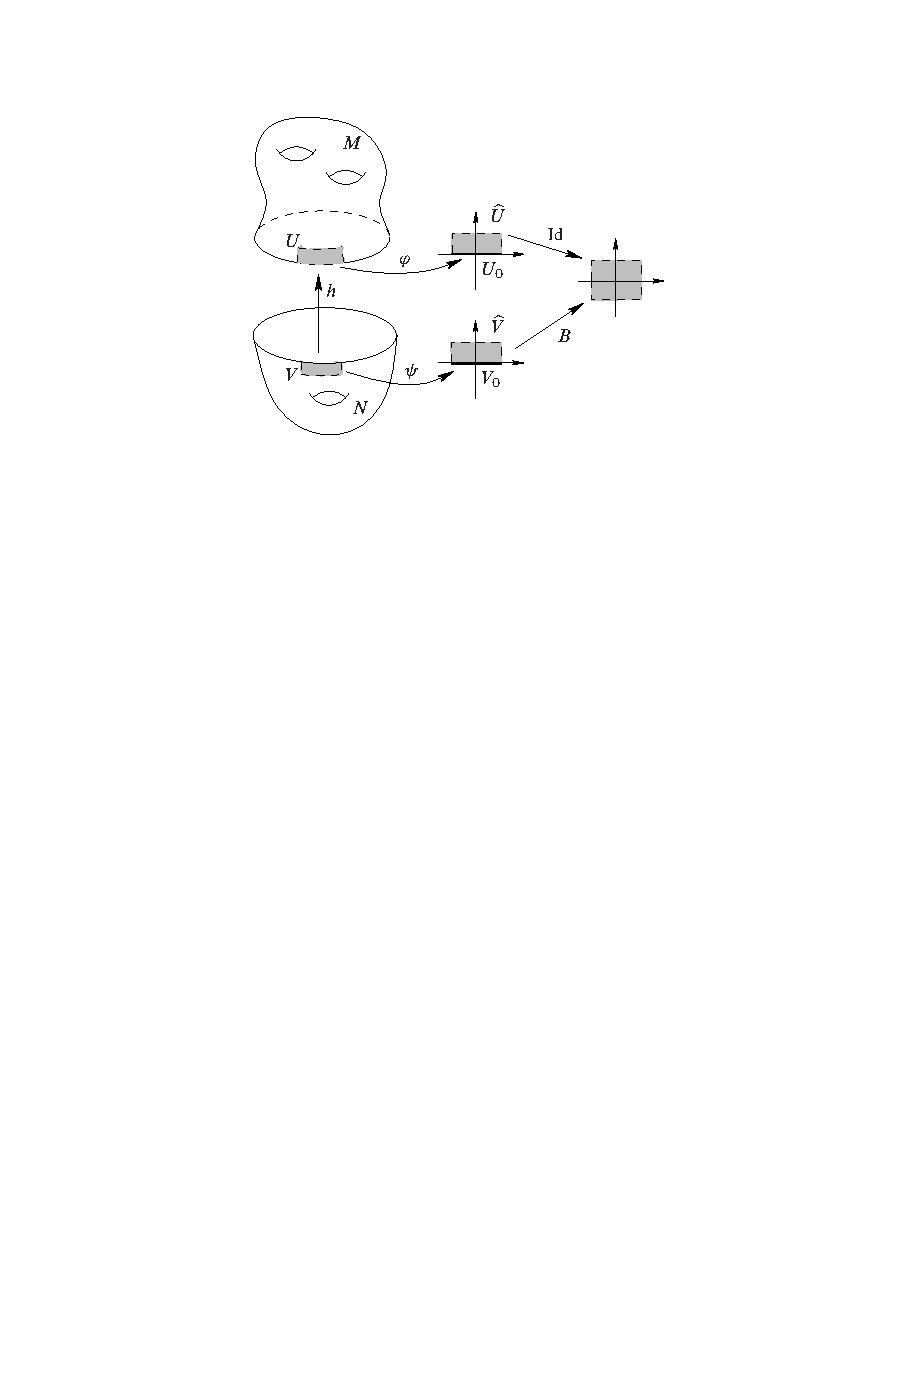
\includegraphics{pictures/attach-manifold}
\caption{Attaching along boundaries.}
\end{figure}

Suppose $s\in S$, and let $y\in\partial N$ and $x=h(y)\in\partial M$ be the two points in the fiber $q^{-1}(s)$. We can choose coordinate charts $(U,\varphi)$ for $M$ and $(V,\psi)$ for $N$ such that $x\in U$ and $y\in V$, and let $\widehat{U}=\varphi(U)$, $\widehat{V}=\psi(V)$. It is useful in this proof to identify $\H^n$ with $\R^{n-1}\times[0,+\infty)$ and $\R^n$ with $\R^{n-1}\times\R$. By shrinking $U$ and $V$ if necessary, we may assume that $h(V\cap\partial N)=U\cap\partial M$, and that $\widehat{U}=U_0\times[0,\eps)$ and $\widehat{V}=V_0\times[0,\eps)$ for some $\eps>0$ and some open subsets $U_0,V_0\sub\R^{n-1}$. Then we can write the coordinate maps as 
\[\varphi(x)=(\varphi_0(x),\varphi_1(x)),\quad\psi(y)=(\psi_0(y),\psi_1(y))\]
for some continuous maps $\varphi_0:U\to U_0$, $\varphi_1:U\to[0,\eps)$, $\psi_0:V\to V_0$ and $\psi_1:V\to[0,\eps)$. Our assumption that $x$ and $y$ are boundary points means that $\varphi_1(x)=\psi_1(y)=0$.\par
We wish to assemble these two charts into a map whose image is an open subset of $\R^n$, by matching them up along corresponding points in $\partial M$ and $\partial N$. As they stand, however, the maps $\varphi$ and might not take corresponding boundary points to the same image point, so we need to adjust for that. Both of the restrictions
\[\varphi_0|_{U\cap\partial M}:U\cap\partial M\to U_0,\quad \psi_0|_{V\cap\partial N}:V\cap\partial N\to V_0\]
are homeomorphisms. Define a homeomorphism $\tau:V_0\to U_0$ by
\[\tau=(\varphi_0|_{U\cap\partial M})\circ h\circ(\psi_0|_{V\cap\partial N})^{-1},\]
and let $B:\widehat{V}\to\R^n$ be the map
\[B(x_1,\dots,x_n)=(\tau(x_1,\dots,x_{n-1}),-x_n).\]
Geometrically, $B$ rearranges the boundary points according to the map $\tau$, and then "flips" each vertical line segment above a boundary point to a line segment below the image point. Our construction ensures that for $y\in\partial N$,
\begin{align}\label{attach manifold with boundary-1}
B\circ\psi(y)=(\tau\circ\psi(y),0)=(\varphi_0\circ h(y),0)=\varphi\circ h(y).
\end{align}
Now define $\widetilde{\varPhi}:U\amalg V\to\R^n$ by
\[\widetilde{\varPhi}=\begin{cases}
\varphi(y),&y\in U;\\
B\circ\psi(y),&y\in V.
\end{cases}\]
Because $U\amalg V$ is a saturated open subset of $M\amalg N$, the restriction of $q$ to it is a quotient map onto the neighborhood $q(U\amalg V)$ of $s$, and $(\ref{attach manifold with boundary-1})$ shows that $\widetilde{\varPhi}$ passes
to the quotient and defines an injective continuous map $\varPhi:q(U\amalg V)\to\R^n$. Since $\varphi$, $\psi$, and $B$ are homeomorphisms onto their images, we can define an inverse for $\varPhi$ as follows:
\[\varPhi^{-1}(y)=\begin{cases}
q\circ\varphi^{-1}(y),&y^n\geq 0;\\
q\circ\psi^{-1}\circ B^{-1}(y)&y^n\leq 0.
\end{cases}\]
These two definitions agree where they overlap, so the resulting map is continuous by the gluing lemma. Thus $\varPhi$ is a homeomorphism. Note that the image of $\varPhi$ is exactly $U_0\times(-\eps,\eps)$, which is open in $\R^n$. Therefore $M\cup_hN$ is locally Euclidean of dimension $n$.\par
The quotient space $M\cup_h N$ is second countable by Proposition~\ref{manifold quotient is manifold}. To prove that it is Hausdorff, we need to show that the fibers of $q$ can be separated by saturated open subsets. It is straightforward to check on a case-by-case base that the preimages of sufficiently small coordinate balls will do.\par
It follows immediately from Proposition~\ref{adjunction space prop}(a) that the quotient map $q$ restricts to a topological embedding of $M$ into $M\cup_h N$ with closed image. On the other hand, because $h$ is a homeomorphism, it is easy to see that $M\cup_h N$ is also equal to
$N\cup_{h^{-1}}M$, so $q$ also restricts to a topological embedding of $N$ with closed image. The union of the images of these embeddings is all of $M\cup_hN$, and their intersection is the set $S$ defined above, which is exactly the image of either boundary.
\end{proof}
Here is an important example of the preceding construction.
\begin{example}[\textbf{The Double of a Manifold with Boundary}]
Suppose $M$ is an ndimensional manifold with boundary. If $h:\partial M\to \partial M$ is the identity map, the resulting quotient space $M\cup_{h}M$ is denoted by $D(M)$ and called the \textbf{double of $\bm{M}$}. It can be visualized as the space obtained by attaching two copies of $M$ to each other along their common boundary. (If $\partial M=\emp$, then $D(M)$ is just the disjoint union of two copies of $M)$
\end{example}
The following proposition is an immediate consequence of Theorem~\ref{attach manifold with boundary}.
\begin{proposition}
Every $n$-manifold with boundary is homeomorphic to a closed subset of an $n$-manifold without boundary.
\end{proposition}
This construction can be used to extend many results about manifolds to manifolds with boundary. For example, any property that holds for all closed subsets of manifolds is also shared by manifolds with boundary.
\section{Paracompactness}
\subsection{Paracompact spaces}
Let $X$ be a topological space. A collection $\mathcal{A}$ of subsets of $X$ is said to be \textbf{locally finite} if each point of $X$ has a neighborhood that intersects at most finitely many of the sets in $\mathcal{A}$. Given a cover $\mathcal{A}$ of $X$, another cover $\mathcal{B}$ is called a \textbf{refinement} of $\mathcal{A}$ if for each $B\in\mathcal{B}$ there exists some $A\in\mathcal{A}$ such that $B\sub A$. It is an \textbf{open refinement} if each $B\in\mathcal{B}$ is an open subset of $X$. (Note that every subcover of $\mathcal{A}$ is a refinement of $\mathcal{A}$, but a refinement is not in general a subcover, because a refinement does not need to be composed of sets that are elements of $\mathcal{A}$.)\par
Here are some elementary properties of local finiteness. Given a collection $\mathcal{A}$ of subsets of a topological space, let us use the notation $\widebar{\mathcal{A}}$ to denote the collection of
closures of sets in $\mathcal{A}$:
\[\widebar{\mathcal{A}}:=\{\widebar{A}:A\in\mathcal{A}\}\]
\begin{lemma}\label{topological space locally iff closure is locally finite}
Let $X$ be a topological space and $\mathcal{A}$ be a collection of subsets of X. Then $\mathcal{A}$ is locally finite if and only $\widebar{\mathcal{A}}$ is locally finite.
\end{lemma}
\begin{proof}
If $\widebar{\mathcal{A}}$ is locally finite, then it follows immediately that $\mathcal{A}$ is locally finite. Conversely, suppose $\mathcal{A}$ is locally finite. Given $x\in X$, let $W$ be a neighborhood of $x$ that intersects only finitely many of the sets in $\mathcal{A}$, say $A_1,\dots,A_n$. If $W$ contains a point $a$ in $\widebar{A}$ for some $A\in\mathcal{A}$, then $W\cap A\neq\emp$ since $a$ is a limit point of $A$. It then follows that $A$ is one of the sets $A_1,\dots,A_n$, and therefore $W$ can only intersects finitely many sets in $\widebar{\mathcal{A}}$.
\end{proof}
\begin{lemma}\label{topological space locally finite family closure and union}
If $\mathcal{A}$ is a locally finite collection of subsets of $X$, then
\[\widebar{\bigcup_{A\in\mathcal{A}} A}=\bigcup_{A\in\mathcal{A}}\widebar{A}\]
\end{lemma}
\begin{proof}
The right-hand side is contained in the lefthand side even without the assumption of local finiteness, so we only prove the reverse containment. We will prove the contrapositive: assuming $x\in X$ is not an element of $\bigcup_{A\in\mathcal{A}}\widebar{A}$, we show it is not an element of $\widebar{\bigcup_{A\in\mathcal{A}} A}$ either. By Lemma~\ref{topological space locally iff closure is locally finite},
$x$ has a neighborhood $U$ that intersects only finitely many sets in $\widebar{A}$, say $\widebar{A}_1,\dots,\widebar{A}_k$. Then $U\setminus(\widebar{A}_1\cap\cdots\cap\widebar{A}_1)$ is a neighborhood of $x$ that intersects none of the sets in $\mathcal{A}$, so $x\notin\widebar{\bigcup_{A\in\mathcal{A}} A}$.
\end{proof}
\begin{definition}
A space $X$ is said to be \textbf{paracompact} if every open cover of $X$ admits a locally finite open refinement. Every compact space is paracompact, because a finite subcover is a locally finite open refinement.
\end{definition}
\begin{proposition}
A closed subspace of a paracompact space is paracompact.
\end{proposition}
\begin{proof}
If $A$ is a closed subspace of a paracompact space $X$, every open cover of $A$ is of the form $\{U_\alpha\}\cap A$, where $U_\alpha$ are open in $X$. Add in the open set $X-A$, we get an open cover of $X$, thus using paracompactness of $X$ we get the claim.
\end{proof}
A key topological fact about manifolds, as we show below, is that they are all paracompact. This is a consequence of second countability, and in fact is one of the most important reasons why second countability is included in the definition of manifolds. For spaces that are Hausdorff and locally Euclidean with countably many components, the two conditions are equivalent.\par
Before we prove that manifolds are paracompact, we need a preliminary result. If $X$ is a topological space, a sequence $\{K_i\}_{i\in\N}$ of compact subsets of $X$ is called an \textbf{exhaustion} of $X$ by compact sets if $X=\bigcup_{i}K_i$ and $K_i\sub\Int K_{i+1}$ for each $i$.
\begin{proposition}\label{exhaustion by compact}
A $\sigma$-compact locally compact Hausdorff space admits an exhaustion by compact sets.
\end{proposition}
\begin{proof}
Since $X$ is a $\sigma$-compact, there exists a sequence $\{K_i\}$ of compact subsets such that $X=\bigcup_iK_i$. Every compact subset of $X$ has a precompact open neighborhood by Proposition~\ref{LCH precompact nbhd for compact set}. Thus we may take $U_1$ to be a precompact open neighborhood of $K_1$, and then, proceeding inductively, take $U_n$ to be a precompact open neighborhood of $\widebar{U}_{i-1}\cup K_i$. It follows that the sequence $\{U_i\}$ satisfies $K_i\sub U_i$ and $\widebar{U}_{i}\sub U_{n+1}$. Let $\widetilde{K}_i=\widebar{U}_i$, then $\{\widetilde{K}_i\}$ is a exhaustion of $X$ by compact sets. 
\end{proof}
\begin{theorem}\label{loc compact paracompact}
Every $\sigma$-compact locally compact Hausdorff space is paracompact. In fact, given such a space $X$, an open cover $\mathcal{U}$ of $X$, and any base $\mathcal{B}$ for the topology of $X$, there exists a countable, locally finite open refinement of $\mathcal{U}$ consisting of elements of $\mathcal{B}$.
\end{theorem}
\begin{proof}
Given $X,\mathcal{U}$ and $\mathcal{B}$, by Proposition~\ref{exhaustion by compact}, let $(K_i)_{i\in\N}$ be an exhaustion of $X$ by compact sets. For each $i$, let
\[V_i=K_{i+1}\setminus\Int K_i,\quad W_i=\Int K_{i+2}\setminus K_{i-1}\]
where we interpret $K_i=\emp$ if $i<1$. Then $V_i$ is a compact set contained in the open subset $W_i$. For each $x\in V_i$, there is some $U_x\in\mathcal{U}$ containing $x$, and because $\mathcal{B}$ is a base, there exists $B_x\in\mathcal{B}$ such that $x\in B_x\sub U_x\cap W_i$. The collection of all such sets $B_x$ as $x$ ranges over $V_i$ is an open cover of $V_i$, and thus has a finite subcover. The union of all such finite subcovers as $i$ ranges over the positive integers is a countable open cover of $M$ that refines $\mathcal{U}$. Because the finite subcover of $V_i$ consists of sets contained in $W_i$, and $W_i\cap W_{j}\neq \emp$ only for $i-2<j<i+2$, the resulting cover is locally finite.
\end{proof}
In view of the theorem, one may wonder the connection between paracompactness and $\sigma$-compactness for a locally Hausdorff space. The following theorem answers this question.
\begin{theorem}\label{LCH paracompact iff sigma-compact}
A locally compact Hausdorff space $X$ is paracompact if and only if it is a disjoint union of open $\sigma$-compact subsets.
\end{theorem}
\begin{proof}
Assume that $X$ is paracompact. Using local compactness, cover the space with open precompact sets $U_\alpha$. Using paracompactness we may assum this cover is locally finite. We shall inductively construct open precompact sets $V_i$. We start with $V_1=U_\beta$ for some given $\beta$. If $V_i$ has been defined then consider all the $U_\alpha$ which intersect $\widebar{V}_i$: By compactness of $\widebar{V}_i$ and the local finiteness of the cover, this set of $U_\alpha$'s is finite. Let $V_{i+1}$ be the union of these $U_\alpha$. Then $\widebar{V}_{i+1}$ is the union of the closures of this finite set of $U_\alpha$'s and so it is compact. Also $\widebar{V}_i\sub V_{i+1}$. Put $V=\bigcup_iV_i$, then $V$ is open. By Lemma~\ref{topological space locally finite family closure and union} $\widebar{V}$ is the union of the closures of these $U_\alpha$'s. But by construction each of these closures is contained in some $\widebar{V}_i\sub V_{i+1}\sub V$. Thus $V=\widebar{V}$ is closed and by construction, is $\sigma$-compact. Now since $V$ is closed and open, it is a connected component of $X$. Thus $X$ is a disjoint union of open $\sigma$-compact subsets.\par
Conversely, assume that $X$ is a union of $\sigma$-compact subsets. It is clear that a disjoint union of open paracompact spaces is paracompact, and so we may as well assume the space $X$ to be $\sigma$-compact. Let $X=\bigcup_iC_i$ where the $C_i$ are compact. We define an exhaustion of $X$ by compact sets $K_i$.
\begin{itemize}
\item Let $K_1=C_1$. To define $K_2$, for each point $x\in C_1$ we find by local compactness a precompact neighborhood $U_x$ of $x$. Then the collection $\{U_x\}$ covers $C_1$, hence has a subcover $\{U^{(1)}_{1},\dots,U^{(1)}_{i_1}\}$. We set
\[K_2=C_2\cup\bigcup_{j=1}^{i_1}\widebar{U}^{(1)}_j\]
so $K_2$ is compact and $K_1\sub\Int K_2$.
\item Assume the ascending compact sets $K_1,\dots,K_n$ are defined. Now by the same argument we find precompact sets $\{U^{(n)}_1,\dots,U^{(n)}_{i_n}\}$ covers $K_n$. Then we set
\[K_{n+1}=C_n\cup\bigcup_{j=1}^{i_n}\widebar{U}_j^{(n)}\] 
Now $K_{n+1}$ is compact and $K_n\sub\Int K_{n+1}$. By induction we get the sequence $\{K_i\}$, and since each $C_i$ is contained in $K_i$, we have $X=\bigcup_iK_i$.
\end{itemize}
Now with this exhaustion by compact sets, by arguing as in the proof of Theorem~\ref{loc compact paracompact}, we can show that $X$ is paracompact.
\end{proof}
One feature of paracompact Hausdorff spaces is that they satisfy a strengthened version of the Hausdorff property. A topological space $X$ is said to be \textbf{normal} if it is Hausdorff and for every pair of disjoint closed subsets $A,B\sub X$, there exist disjoint open subsets $U,V\sub X$ such that $A\sub U$ and $B\sub V$. Similarly, $X$ is said to be \textbf{regular} if it is Hausdorff and for every closed subset $B\sub X$ and point $a\in B$, there exist disjoint open subsets $U,V\sub X$ such that $a\in U$ and $B\sub V$. Briefly, in normal spaces, closed subsets can be separated by open subsets; and in regular spaces, closed subsets can be separated from points by open subsets.
\begin{lemma}\label{Hausdorff normal iff}
Let $X$ be a Hausdorff space. Then $X$ is normal if and only if it satisfies the following condition: whenever $A$ is a closed subset of $X$ and $U$ is a neighborhood of $A$, there exists a neighborhood $V$ of $A$ such that $\widebar{V}\sub U$.
\end{lemma}
\begin{proof}
This is easily seen to be equivalent to the definition of normality by taking
$B=U^c$.
\end{proof}
\begin{theorem}\label{para is normal}
Every paracompact Hausdorff space is normal.
\end{theorem}
\begin{proof}
Suppose $X$ is a paracompact Hausdorff space, and let $A$ and $B$ be disjoint closed subsets of $X$. We begin with the special case in which $B=\{q\}$ is a singleton; in other words, we prove that $X$ is regular.\par
For each $p\in A$, because $X$ is Hausdorff there exist disjoint open subsets $U_p$ and$V_p$ such that $p\in U_p$ and $q\in V_p$. The collection $\{U_p:p\in A\}\cup\{X\setminus A\}$ is an open cover of $X$. By paracompactness, it has a locally finite open refinement $\mathcal{W}$. Each of the open subsets in $\mathcal{W}$ is contained either in $U_p$ for some $p$, or in $X\setminus A$. Let $\mathcal{U}$ be the collection of all the sets in $\mathcal{W}$ that are contained in some $U_p$. Then $\mathcal{U}$ is
still locally finite, and it is an open cover of $A$. Moreover, if $U\in\mathcal{U}$, then there is a neighborhood $V_p$ of $q$ disjoint from $U$, so $\widebar{U}$ does not contain $q$.\par
Let $\mathfrak{U}=\bigcup_{U\in\mathcal{U}}U$, and $\mathfrak{V}=X\setminus \mathfrak{U}$. Because $\mathcal{U}$ is locally finite, $\widebar{\mathfrak{U}}=\bigcup_{U\in\mathcal{U}}\widebar{U}$
by Lemma~\ref{topological space locally finite family closure and union}. Thus $q\notin\widebar{\mathfrak{U}}$, so $\mathfrak{U}$ and $\mathfrak{V}$ are disjoint open subsets of $X$ containing $A$ and $q$, respectively. This completes the proof that $X$ is regular. Next consider arbitrary disjoint closed subsets $A$ and $B$. Exactly the same argument
works in this case, using regularity in place of the Hausdorff condition.
\end{proof}
The following result is a nontrivial property about normal spaces.
\begin{theorem}[\textbf{Urysohn's Lemma}]\label{Urysohn lemma}
Suppose $X$ is a normal topological space. If $A,B\sub X$ are disjoint closed subsets, then there exists a continuous function $f:X\to[0,1]$ such that $f|_A\equiv0$ and $f|_B\equiv1$.
\end{theorem}
\begin{proof}We will construct for each rational number $r$ an open subset $U_r\sub X$, such
that the following properties hold
\begin{itemize}
\item[(a)] $U_r=\emp$ when $r<0$, and $U_r=X$ when $r>1$.
\item[(b)] $A\sub U_0$.
\item[(c)] $U_1=X\setminus B$.
\item[(d)] If $p<q$, then $\widebar{U}_p\sub U_q$
\end{itemize}
we will do this by induction. We begin by defining $U_1=X\setminus B$, and defining $U_r$ for $r\notin [0,1]$ by (a). By normality, there exists a neighborhood $U_0$ of $A$ such that $\widebar{U}_0\sub U_1$. Let $\{r_i\}_{i\in\N}$ be a enumeration of the rationals in $[0,1]$. By normality again, there exists an open subset $U_{r_1}\sub X$ such that $\widebar{U}_0\sub U_{r_1}$ and $\widebar{U}_{r_1}\sub U_1$. Now use induction, suppose $U_i$ has been defined for $i=1,\dots,n$ such that $\widebar{U}_0\sub U_{r_i}$, $\widebar{U}_{r_{i}}\sub U_1$ and $\widebar{U}_{r_{i}}\sub U_{r_{j}}$ for $r_i<r_j$. Consider the next rational number $r_{n+1}$ in the sequence, and let $p$ be the largest number in the set $\{0,r_1,\dots,r_n,1\}$ that is smaller than $r_{n+1}$, and $q$ the smallest number in the same set that is larger than $r_{n+1}$. Then $\widebar{U}_p\sub U_q$ By normality, there exists an open subset $U_{r_{n+1}}$ such that $\widebar{U}_{p}\sub U_{r_{n+1}}$ and $\widebar{U}_{r_{n+1}}\sub U_q$. Continuing by induction, we obtain open subsets $U_r$ for all rational $r$ satisfying the properties above.\par
Now, define $f:X\to\R$ by
\[f(x)=\inf\{r\in\Q:x\sub U_r\}.\]
Because of (a), $f$ is well defined and takes its values in $[0,1]$. Properties (a) and (b)
imply that $f(x)=0$ for $x\in A$, and (a) and (c) imply that $f(x)=1$ for $x\in B$. Thus
it remains only to show that $f$ is continuous.\par
Because sets of the form $(a,\infty)$ and $(-\infty,a)$ form a subbase for the topology of $\R$, it suffices to show that the preimage under $f$ of any such set is open. We begin with the following observations:
\begin{align}
&f(x)<a \iff x\in U_r\text{ for some rational }r<a\label{Urysohn-1}\\
&f(x)\leq a \iff x\in \widebar{U}_r\text{ for any rational }r>a\label{Urysohn-2}
\end{align}
The equivalence $(\ref{Urysohn-1})$ is an easy consequence of the definition of $f$. To prove $(\ref{Urysohn-2})$, suppose first that $f(x)\leq a$. If $r$ is any rational number greater than $a$, then by
definition of $f$, there is a rational number $s<r$ such that $x\in U_s\sub U_r\sub\widebar{U}_r$. Conversely, suppose $x\in\widebar{U}_r$ for every rational number greater than $a$. If $s>a$ is rational, choose a rational number $r$ such that $s>r>a$; it follows from our hypothesis that
$x\in\widebar{U}_r\sub U_s$, which implies that $f(x)\leq s$. Since this is true for every rationals $s>a$, it follows that $f(x)\leq a$.\par
From $(\ref{Urysohn-1})$ and $(\ref{Urysohn-2})$ we conclude that
\[f^{-1}\big((-\infty,a)\big)=\bigcup_{\substack{r\in\Q\\r<a}}U_r,\quad f^{-1}\big((a,\infty)\big)=X\setminus\bigcap_{\substack{r\in\Q\\r>a}}\widebar{U}_r\]
both of which are open. Thus $f$ is continuous.
\end{proof}
The next corollary of Urysohn's lemma is often the most useful. If $X$ is a topological space and $f:X\to \R$ is a continuous function, the support of $f$, denoted by $\supp(f)$, is the closure of the set $\{x\in X:f(x)\neq 0\}$:
\[\supp(f):=\widebar{\{x\in X:f(x)\neq 0\}}\]
If $A$ is a closed subset of $X$ and $U$ is a neighborhood of $A$, a continuous function $f:X\to[0,1]$ such that $f|_A\equiv1$ and $\supp(f)\sub U$ is called a \textbf{bump function} for $A$ supported in $U$.
\begin{theorem}
Let $X$ be a normal space. If $A$ is a closed subset of $X$ and $U$ is a neighborhood of $A$, there exists a bump function for $A$ supported in $U$.
\end{theorem}
\begin{proof}
Just apply Urysohn's Lemma with $B=X\setminus U$.
\end{proof}
One immediate consequence of the Urysohn lemma is the useful theorem called the Tietze extension theorem. It deals with the problem of extending a continuous realvalued function that is defined on a subspace of a space $X$ to a continuous function defined on all of $X$. This theorem is important in many of the applications of topology.
\begin{theorem}[\textbf{Tietze extension theorem}]
Let $X$ be a normal space and $A$ be a closed subspace of $X$.
\begin{itemize}
\item[(a)] Any continuous map of $A$ into a closed interval $[a,b]$ may be extended to a continuous map of all of $X$ into $[a,b]$.
\item[(b)] Any continuous map of $A$ into $\R$ may be extended to a continuous map of all of $X$ into $\R$.
\end{itemize}
\end{theorem}
\begin{proof}
We first prove (a). The idea of the proof is to construct a sequence of continuous functions $g_n$ defined on the entire space $X$, such that the sequence $g_n$ converges uniformly, and such that the restriction of $g_n$ to $A$ approximates $f$ more and more closely as $n$ becomes large. Then the limit function will be continuous, and its restriction to $A$ will equal $f$.\par
Without loss of generality, we may assume that $[a,b]=[0,1]$. We claim that there is a sequence $\{g_n:X\to [0,2^{n-1}/3^n]\}$ of continuous functions such that $0\leq f-\sum_{i=1}^{n}g_i\leq 2^{n-1}/3^n$ on $A$. To begin with, let $B=f^{-1}([0,1/3])$ and $C=f^{-1}([2/3,1])$. These are closed subsets of $A$, and since $A$ itself is closed, they are closed in $X$. By Urysohn's lemma there is a continuous $g_1:X\to [0,1/3]$ with $g_1=0$ on $B$ and $g_1=1/3$ on $C$; it follows that $0\leq f-g_1\leq 2/3$ on $A$. In general, having found $g_1,\dots,g_{n-1}$, by the same reasoning we can find $g_{n}:X\to[0,2^{n-1}/3^n]$ such that $g_n=0$ on the set where $f-\sum_{i=1}^{n-1}g_i\leq 2^{n-1}/3^n$ and $g_n=2^{n-1}/3^n$ on the set where $f-\sum_{i=1}^{n-1}g_i\geq (2/3)^n$. Let $F=\sum_{n=1}^{\infty}g_n$. Since $|g_n|\leq 2^{n-1}/3^n$, the partial sums of this series converge uniformly, so $F$ is continuous. Moreover, on $A$ we have $0<f-F<(2/3)^n$ for all $n$, whence $F=f$ on $A$.\par
We now prove part (b) of the theorem, in which $f$ maps $A$ into $\R$. We can replace $\R$ by the open interval $(0,1)$, since this interval is homeomorphic to $\R$. So let $f$ be a continuous map from $A$ into $(0,1)$. The half of the Tietze theorem already proved shows that we can extend $f$ to a continuous map $F:X\to[0,1]$ mapping $X$ into the closed interval. Let us define a subset $D$ of $X$ by the equation
\[D=F^{-1}(0)\cup F^{-1}(1).\]
Since $F$ is continuous, $D$ is a closed subset of $X$. Because $F(A)=f(A)$, which is contained in $(0,1)$, the set $A$ is disjoint from $D$. By the Urysohn lemma, there is a continuous function $\phi:X\to[0,1]$ such that $\phi(D)=\{0\}$ and $\phi(A)=\{1\}$. Define
\[\widetilde{F}=F(x)\phi(x).\]
Then $\widetilde{F}$ is continuous, being the product of two continuous functions. Also, $\widetilde{F}$ is an extension of $F$ with values in $(0,1)$. This finishes the proof.
\end{proof}
\subsection{Partitions of unity}
The applications of paracompactness are all based on a technical tool called a partition of unity, which can be used to blend together locally defined continuous maps into a global one.\par
For this purpose, we need to consider open covers indexed by some set. (Of course any open cover $\mathcal{U}$ can be considered as an indexed family, just by taking the index set to be $\mathcal{U}$ itself.) In this context, an indexed family $\mathcal{U}=(U_\alpha)_{\alpha\in A}$ of subsets of a topological space $X$ is said to be a \textbf{locally finite} family if each point of $X$ has a neighborhood that intersects $U_\alpha$ for at most finitely many values of $\alpha$.\par
If $\mathcal{U}=(U_\alpha)_{\alpha\in A}$ is an indexed open cover of $X$, a \textbf{partition of unity} subordinate to $\mathcal{U}$ is a family of continuous functions $\psi_\alpha:X\to\R$, indexed by the same set $A$, with the following properties:
\begin{itemize}
\item[(\rmnum{1})] $0\leq\psi_\alpha(x)\leq 1$ for all $\alpha\in A$ and all $x\in X$.
\item[(\rmnum{2})] $\supp(\psi_\alpha)\sub U_\alpha$.
\item[(\rmnum{3})] The family of supports $\{\supp(\psi_\alpha)\}_\alpha\in A$ is locally finite.
\item[(\rmnum{4})] $\sum_{\alpha\in A}\psi_\alpha(x)=1$ for all $x\in X$.
\end{itemize}
Because of the local finiteness condition (\rmnum{3}), the sum in (\rmnum{4}) has only finitely many nonzero terms in a neighborhood of each point, so there is no issue of convergence.\par
First we have a simple observation.
\begin{proposition}\label{partition of unity para}
Suppose $X$ is a topological space with the property that for every indexed open cover $\mathcal{U}$ of $X$, there exists a partition of unity subordinate to $\mathcal{U}$. Then $X$ is paracompact.
\end{proposition}
\begin{proof}
Let $\mathcal{U}=\{U_\alpha\}_{\alpha\in A}$ be any cover of $X$, and $\{\psi_\alpha\}_{\alpha\in A}$. Then since $\sum_{\alpha\in A}\psi_\alpha=1$, the collection $\{\supp(\psi_\alpha)\}_{\alpha\in A}$ covers $X$. Moreover, by definition this collection is a locally finite refinement of $\mathcal{U}$. Thus $X$ is paracompact.
\end{proof}
Now we want to prove the converse of Proposition~\ref{partition of unity para}. First we need some lemmas.
\begin{lemma}\label{part refin lem}
Suppose $X$ is a paracompact Hausdorff space. If $\mathcal{U}=(U_\alpha)_{\alpha\in A}$ is an indexed open cover of $X$, then $\mathcal{U}$ admits a locally finite open refinement $\mathcal{V}=(V_\alpha)_{\alpha\in A}$ indexed by the same set, such that $\widebar{V}_\alpha\sub U_\alpha$ for each $\alpha$.
\end{lemma}
\begin{proof}
By Lemma~\ref{Hausdorff normal iff} and Theorem~\ref{para is normal}, each $x\in X$ has a neighborhood $Y_x$ such that $\widebar{Y}_x\sub U_\alpha$ for some $\alpha\in A$. Since $X$ is paracompact, the open cover $\{Y_x:x\in X\}$ has a locally finite open refinement. Let us index this refinement by some set $B$, and denote it by $\mathcal{Z}=(Z_\beta)_{\beta\in B}$. For each $\beta$,there is some $x\in X$ such that $Z_\beta\sub Y_x$, and therefore there is some $\alpha\in A$ such that
$\widebar{Z}_\beta\sub \widebar{Y}_x\sub U_\alpha$. Define a function $a:B\to A$ by choosing some such index $\alpha\in A$ for each $\beta\in B$, and setting $a(\beta)=\alpha$.\par
For each $\alpha\in A$, define an open subset $V_\alpha\sub X$ by
\[V_\alpha=\bigcup_{a(\beta)=\alpha}Z_\beta\]
(If there are no indices $\beta$ such that $a(\beta)=\alpha$, then $V_\beta=\emp$.) Because the family $\mathcal{Z}$ is locally finite, the closure of $V_\alpha$ is equal to $\bigcup_{a(\beta)=\alpha}\widebar{Z}_{\beta}$ by Lemma~\ref{topological space locally finite family closure and union}, which is contained in $U_\alpha$ as required.
\end{proof}
\begin{theorem}[\textbf{Existence of Partitions of Unity}]\label{partition of unity}
Let $X$ be a paracompact Hausdorff space. If $\,\mathcal{U}$ is any indexed open cover of $X$, then there is a partition of unity subordinate to $\mathcal{U}$.
\end{theorem}
\begin{proof}
Let $\mathcal{U}=(U_\alpha)_{\alpha\in A}$ be an indexed open cover of $X$. Apply Lemma~\ref{part refin lem} twice, we obtain locally finite open covers $\mathcal{V}=(V_\alpha)_{\alpha\in A}$ and $\mathcal{W}=(W_\alpha)_{\alpha\in A}$ such that $\widebar{W}_\alpha\sub V_\alpha$ and $\widebar{V}_\alpha\sub U_\alpha$.\par
Now, for each $\alpha\in A$, let $f_\alpha:X\to[0,1]$ be a bump function for $\widebar{W}_\alpha$ supported in $V_\alpha$. Define $f:X\to\R$ by $f(x)=\sum_\alpha f_\alpha(x)$. Because $\supp(f_\alpha)\sub V_\alpha$, the family of supports $\{\supp(f_\alpha)\}_{\alpha\in A}$ is locally finite; thus each point of $X$ has a neighborhood on which only finitely many terms of this sum are nonzero, so $f$ is continuous. Because
the sets $\{W_\alpha\}$ cover X, for each $x\in X$ there is at least one $\alpha$ such that $x\in W_\alpha$ andthus $f_\alpha(x)=1$, so $f$ is everywhere positive. Therefore, we can define 
\[\psi_\alpha(x)=\dfrac{f_\alpha(x)}{f(x)}\]
Then $\{\psi_\alpha\}_{\alpha\in A}$ is the desired partition of unity, as one may check.
\end{proof}
\begin{theorem}[\textbf{Embeddability of Compact Manifolds}]
Every compact manifold is homeomorphic to a subset of some Euclidean space.
\end{theorem}
\begin{proof}
Suppose $M$ is a compact $n$-manifold. By compactness we can obtain a cover of $M$ by finitely many open subsets $U_1,\dots,U_k$, each of which is homeomorphic to $\R^n$. For each $i$, let $\varphi_i:U_i\to\R^n$ be a homeomorphism. Let $\{\psi_i\}$ be a partition of unity subordinate to this cover, and define functions $F_i:M\to \R^n$ by
\[F_i(x)=\left\{\begin{array}{cl}
\psi_i(x)\varphi_i(x), &x\in U_i\\
0, &x\in M\setminus \supp(\psi_i)
\end{array}\right. \]
Each $F_i$ is continuous by the pasting lemma.\par
Now define $F:M\to \R^{nk+k}$ by
\[F(x)=\big(F_1(x),\dots,F_k(x),\psi_1(x),\dots,\psi_k(x)\big)\] 
Then $F$ is continuous, and if we can show it is injective, it is a topological embedding
by the closed map lemma.\par
Suppose $F(x)=F(y)$ for some points $x,y\in M$. Since $\sum_i\psi_i(x)\equiv1$, there is some $i$ such that $\psi_i(x)>0$ and therefore $x\in U_i$. Because $F(x)=F(y)$ implies $\psi_i(y)=\psi_i(x)>0$, it follows that $y\in U_i$ as well. Then we see that $F_i(x)=F_i(y)$ implies $\varphi_i(x)=\varphi_i(y)$, which in turn implies that $x=y$ since $\varphi_i$ is injective on $U_i$.
\end{proof}
\begin{theorem}
Suppose $M$ is a topological manifold, and $B\sub M$ is any closed subset. Then there exists a continuous function $f:M\to[0,\infty)$ whose zero set is exactly $B$.
\end{theorem}
\begin{proof}
First, consider the special case in which $M=\R^n$ and $B\sub\R^n$ is a closed subset. It is straightforward to check that
\[u(x)=\inf\{|x-y|:y\in B\}\]
does the trick.\par
Now, let $M$ be an arbitrary $n$-manifold and let $B$ be a closed subset of $M$. Let $\mathcal{U}=(u_\alpha)_{\alpha\in A}$ be a cover of $M$ by open subsets homeomorphic to $\R^n$, and
let $\{\psi_\alpha\}_{\alpha\in A}$ be a subordinate partition of unity. For each $\psi_\alpha$ the construction in the preceding paragraph yields a continuous function $u_\alpha:U_\alpha\to [0,\infty)$ such that $u_\alpha^{-1}(0)=B\cap U_\alpha$. Define $f:M\to \R$ by
\[f(x)=\sum_{\alpha\in A}\psi_\alpha(x)u_\alpha(x)\]
where each summand is to be interpreted as zero outside the support of $\psi_\alpha$. Each term in this sum is continuous by the pasting lemma, and only finitely many terms are nonzero in a neighborhood of each point, so this defines a continuous function on $M$. It is easy to check that it is zero exactly on $B$.
\end{proof}
\begin{corollary}
Suppose $M$ is a topological manifold, and $A,B$ are disjoint closed subsets of $M$. Then there exists a continuous function $f:M\to [0,1]$ such that 
\[f^{-1}(0)=A,\quad f^{-1}(1)=B\]
\end{corollary}
\begin{proof}
Using the previous theorem, we can find $u,v: M\to [0,\infty)$ such that $u$ vanishes exactly on $A$ and $v$ vanishes exactly on $B$, and then the function $f(x)=v(x)/\big(u(x)+v(x)\big)$ satisfies the conclusion of the corollary.
\end{proof}
For our last application of partitions of unity, we need the following definition. If $M$ is a topological space, an \textbf{exhaustion function} for $M$ is a continuous function $f:M\to \R$ such that for every $c\in\R$, the sublevel set $f^{-1}\big((-\infty,c]\big)$ is compact. The name comes from the fact that as $k$ ranges through the positive integers, the sublevel sets $f^{-1}\big((-\infty,k]\big)$ form an exhaustion of $M$ by compact sets.
\begin{theorem}[\textbf{Existence of Exhaustion Functions}]\label{exhaustion functions}
Every manifold admits a positive exhaustion function.
\end{theorem}
\begin{proof}
Let $M$ be a manifold, let $\{U_i\}$ be a countable open cover of $M$ by precompact open subsets, and let $\{\psi_i\}$ be a partition of unity subordinate to this cover. Define $f:M\to\R$ by
\[f(x)=\sum_{k=1}^{\infty}k\psi_k(x)\]
Then $f$ is continuous since only finite terms are nonzero in a neighborhood of each point, and positive because $f(x)\geq\sum_{k}\psi_k(x)=1$. For any positive integer $m$, if $x\notin\bigcup_{k=1}^{m}\widebar{U}_k$, then $\psi_k(x)=0$ for $1\leq k\leq m$, so
\[f(x)=\sum_{k=m+1}^{\infty}k\psi_k(x)>\sum_{k=m+1}^{\infty}m\psi_k(x)=m\sum_{k=m+1}^{\infty}\psi_k(x)=m\]
The contrapositive of this last statement is that $f(x)\leq m$ implies $x\in\bigcup_{k=1}^{m}\widebar{U}_k$. Let $c\in\R$ be arbitrary, and let $m$ be any positive integer greater that $c$. It follows that $f^{-1}\big((-\infty,c]\big)$ is a closed subset of the compact set $\bigcup_{k=1}^{m}\widebar{U}_k$, and is therefore compact.
\end{proof}
\section{Uniform structures}
\subsection{Uniform spaces}
\begin{definition}
A \textbf{uniform structure} (or \textbf{uniformity}) on a set $X$ is a structure given by a set $\mathfrak{U}$ of subsets of $X\times X$ whick satisfies the following axioms:
\begin{itemize}
\item[(F1)] If $U\in\mathfrak{U}$ and $U\sub V\sub X\times X$, then $V\in\mathfrak{U}$.
\item[(F2)] If $U\in\mathfrak{U}$ and $V\in\mathfrak{U}$, then $U\cap V\in\mathfrak{U}$.
\item[(U1)] Every set in $\mathfrak{U}$ contains the diagonal $\Delta$.
\item[(U2)] If $U\in\mathfrak{U}$ then $U^{-1}\in\mathfrak{U}$, where $U^{-1}:=\{(y,x):(x,y)\in U\}$ is the \textbf{inverse} of $U$. 
\item[(U3)] If $U\in\mathfrak{U}$ then there is $V\in\mathfrak{U}$ such that $V\circ V\sub U$, where the composite of two sets $V,W\sub X\times X$ is defined by
\[V\circ W:=\{(x,z):\text{there exists $y\in X$ such that $(x,y)\in V$ and $(y,z)\in W$}\}.\]
\end{itemize}
The sets of $\mathfrak{U}$ are called \textbf{entourages} of the uniformity defined on $X$ by $\mathfrak{U}$. A set endowed with a uniformity is called a \textbf{uniform space}.
\end{definition}
If $U$ is an entourage of a uniformity on $X$, we may express the relation $(x,y)\in U$ by saying that "$x$ and $y$ are \textbf{$U$-close}". Note that if $X$ is nonempty then every set in $\mathfrak{U}$ is nonempty by (U1), and (F1) and (F2) impliy that $\mathfrak{U}$ is a filter on $X\times X$. There is only one uniformity on the empty set, namely $\{\emp\}$.\par
Throughout this part we shall also write $V^2$ instead of $V\circ V$, and in general $V^n=V\circ V^{n-1}=V^{n-1}\circ V$, for each integer $n>1$ and each subset $V\sub X\times X$. 
\begin{lemma}\label{uniformity equivalent axiom}
The conjunction of axioms (U2) and (U3) is equivalent (assuming the other axioms of uniform structures) to the following axiom:
\begin{itemize}
\item[(U2')] For each $U\in\mathfrak{U}$ there exists $V\in\mathfrak{U}$ such that $V\circ V^{-1}\sub U$.
\end{itemize}
\end{lemma}
\begin{proof}
Clearly (U2) and (U3) imply (U2'). Conversely, if (U2') is satisfied, then for every $U\in\mathfrak{U}$, there exists $V\in\mathfrak{U}$ such that $V\circ V^{-1}\sub U$, and so
\[V^{-1}=\Delta\circ V^{-1}\sub V\circ V^{-1}\sub U,\]
thus $V\sub U^{-1}$ and by (F1) we have $U^{-1}\in\mathfrak{U}$. This proves (U2). Let $W=V\cap V^{-1}$; then $W\in\mathfrak{U}$ by what we have just proved and (F2), and we have $W\circ W\sub V\circ V^{-1}\sub U$.
\end{proof}
\begin{example}
Let $(X,d)$ be a metric space. Then a uniformity on $X$ is given by subsets of the form
\[U_\eps=\{(x,y):d(x,y)<\eps\}.\]
In this case, $x$ and $y$ are $U_\eps$-close precisely when the distance between $x$ and $y$ is at most $\eps$.
\end{example}
A \textbf{base} or \textbf{fundamental system} of entourages of a uniformity $\mathfrak{U}$ is any set $\mathfrak{B}$ of entourages such that every entourage contains a set belonging to $\mathfrak{B}$.
\begin{example}
Axiom (U3) shows that if $n$ is any positive integer and $V$ runs through  a fundamental system of entourages, then the sets $V^n$ ($n$ times) again form a undamental system of entourages.
\end{example}
Entourages $V$ such that $V=V^{-1}$ are called \textbf{symmetric}. If $V$ is any entourage then $V\cap V^{-1}$ and $V\cup V^{-1}$ are symmetric entourages, and axioms (F2) and (U2) show that the symmetric entourages form a fundamental system of entourages.
\begin{proposition}\label{uniformity base iff}
A set $\mathfrak{B}$ of subsets of $X\times X$ is a fundamental system of entourages of a uniformity $\mathfrak{U}$ on $X$ if and only if $\mathfrak{B}$ is a filterbase and satisfies the following axioms:
\begin{itemize}
\item[(B1)] Every set in $\mathfrak{B}$ contains the diagonal.
\item[(B2)] For every $V\in\mathfrak{B}$ there exists $W\in\mathfrak{B}$ such that $W\sub V^{-1}$. 
\item[(B3)] For every $V\in\mathfrak{B}$ there exists $W\in\mathfrak{B}$ such that $W\circ W\sub V$.
\end{itemize}
\end{proposition}
\begin{proof}
If $\mathfrak{B}$ is a base for a uniformity $\mathfrak{U}$, then $\mathfrak{B}$ clearly satisfies the claimed properties. Conversely, assume the properties for $\mathfrak{B}$, and let $\mathfrak{U}$ be the filter in $X\times X$ generated by $\mathfrak{B}$. We prove that $\mathfrak{U}$ is a uniformity.\par
First, since $\mathfrak{U}$ is a filter, it satisfies (F1) and (F2). Also, by (B1) we see (U1) is satisfies. Now let $U\in\mathfrak{U}$, then $U\sups V$ for some $V\in\mathfrak{V}$. By (B2), there exists $W\in\mathfrak{U}$ such that $W\sub V^{-1}\sub U^{-1}$. Thus $U^{-1}\in\mathfrak{U}$ and (U2) holds. Also, by (B3) there also exists $W'\in\mathfrak{B}$ such that $W'\circ W'\sub V\sub U$. Since $W'\in\mathfrak{U}$, we see (U3) also holds. This completes the proof.
\end{proof}
\begin{example}
Let $X$ be a set and $R$ be an equivalence relation on $X$. Let $\Gamma\sub X\times X$ be the graph of $R$. Then $\Delta\sub\Gamma$ and $\Gamma\circ\Gamma=\Gamma^{-1}=\Gamma$. The set of subsets of $X\times X$ which consists of the set $C$ alone is therefore a fundamental system of entourages of a uniformity on $X$. In particular, if we take $R$ to be the relation of equality, then $C=\Delta$ and the entourages of the corresponding uniformity are all the subsets of $X\times X$ which contain $\Delta$; this uniformity is called the \textbf{discrete uniformity} on $X$, and the set $X$ endowed with this uniformity is called a \textbf{discrete uniform space}.
\end{example}
\begin{example}
On the set $\Z$ of rational integers we can define a uniformity, important in the theory of numbers, as follows: given a prime number $p$, let $U_n$ be the set of all pairs $(x,y)\in\Z\times\Z$ such that $x\equiv y$ mod $p^n$, for each positive integer $n$. It is easily verified that the sets $U_n$ (for a fixed $p$) form a fundamental system of entourages of a uniformity on $\Z$, called the \textbf{$\bm{p}$-adic uniformity}.
\end{example}
Now let $X$ and $Y$ be two sets each endowed with uniformities whose sets of entourages are $\mathfrak{U}$ and $\mathfrak{V}$ respectively, then a bijection $f$ of $X$ onto $Y$ is an isomorphism of the uniformity of $X$ onto that of $Y$ if $(f\times f)(\mathfrak{U})=\mathfrak{V}$.\par
Now we define the topology induced by a uniformity.
\begin{proposition}\label{uniformity induced topology}
Let $X$ be a set endowed with a uniform structure $\mathfrak{U}$, and for each $x\in X$ let $\mathfrak{U}(x)$ be the set of subsets $U(x)$ of $X$, where
\[U(x)=\{y\in X:(x,y)\in V\}\]
and $U$ runs through the set of entourages of $\mathfrak{U}$. Then there is a unique topology on $X$ such that, for each $x\in X$, $\mathfrak{U}(x)$ is the neighbourhood filter of $x$ in this topology.
\end{proposition}
\begin{proof}
We have to show that the $\mathfrak{U}(x)$ satisfy conditions of Proposition~\ref{topological space determined by nbhd filter}. In view of the axoims of uniformity, we only need to prove (U4). To see this, let $V$ be an entourage of $\mathfrak{U}$, $W$ an entourage of $\mathfrak{U}$ such that $W\circ W\sub V$; then if $(x,y)\in W$ and $(y,z)\in W$ we have $(x,z)\in V$, so that $W(y)\sub V(x)$ for all $y\in W(x)$, and therefore $V(x)\in\mathfrak{U}(y)$ for all $y\in W(x)$. This completes the proof.
\end{proof}
The topology defined in Proposition~\ref{uniformity induced topology} is called the \textbf{topology induced by the uniform structure $\mathfrak{U}$}.
\begin{example}
The topology induced by the additive uniformity on the set of real numbers is the topology of the real line. On any set $X$, the topology induced by the discrete uniformity is the discrete topology. The topology induced by the $p$-adic uniformity is the $p$-adic topology on $\Z$.
\end{example}
In the future, when we speak of the topology of a uniform space $X$, we shall always mean the topology induced by the uniform structure of the space, unless the contrary is expressly stated. The topological space obtained by putting this topology on the set $X$ is sometimes called the topological space \textit{underlying} the uniform space in question. For example, when we say that a uniform space is Hausdorff, or compact, or locally compact, etc., we mean that the underlying topological space has this property.\par
If $X$ and $Y$ are two uniform spaces, any isomorphism $f$ of the uniform structure of $X$ onto that of $Y$ is also a homeomorphism of $X$ onto $Y$; we say that $f$ is an \textbf{isomorphism} of the uniform space $X$ onto the uniform space $Y$. It should be noted that a homeomorphism of $X$ onto $Y$ is not necessarily an isomorphism of the uniform structure
of $X$ onto that of $Y$. In other words, distinct uniformities on the same set $X$ can induce the same topology. For example, on $(0,+\infty)$, the additive and the multiplicative uniformities (which are distinct) induce the same topology.
\begin{proposition}\label{uniformity on product space closure char}
Let $X$ be a uniform space. For every symmetric entourage $V$ of $X$ and every subset $S$ of $X\times X$, $V\circ S\circ V$ is a neighbourhood of $S$ in the product space $X\times X$, and the closure of $S$ in this space is given by the formula
\begin{align}\label{uniformity on product space closure char-1}
\widebar{S}=\bigcap_{V\in\mathfrak{S}}V\circ S\circ V
\end{align}
where $\mathfrak{S}$ denotes the set of symmetric entourages of $X$.
\end{proposition}
\begin{proof}
Let $V$ be a symmetric entourage of $X$. The relation $(x,y)\in V\circ S\circ V$ means that there is an element $(p,q)$ of $S$ such that $(x,p)\in V$ and $(q,y)\in V$: in other words ($V$ being symmetric) $x\in V(p)$ andy $y\in V(q)$, that is $(x,y)\in V(p)\times V(q)$. Since $V(p)\times V(q)$ is a neighbourhood of $(p,q)$ in $X\times X$, the first part of the proposition is proved. The relations $(x,p)\in V$, $(y,q)\in V$ can also be written $p\in V(x)$, $q\in V(y)$, or $(p,q)\in V(x)\times V(y)$. As $V$ runs through $\mathfrak{S}$, the sets $V(x)\times V(y)$ form a fundamental system of neighbourhoods of $(x,y)$ in $X\times X$; for if $U$ and $V$ are any two entourages there is always a symmetric entourage $W\sub U\cap V$, so that $W(x)\times W(y)\sub U(x)\times V(y)$. Hence $V(x)\times V(y)$ meets $S$ for each $V\in\mathfrak{S}$ if and only if $(x,y)\in\widebar{S}$ , and formula $(\ref{uniformity on product space closure char-1})$ follows.
\end{proof}
\begin{corollary}\label{uniformity topology closure char}
If $A$ is any subset of $X$ and $V$ is any symmetric entourage of $X$, then $V(A)$ is a neighbourhood of $A$ in $X$, and
\begin{align}\label{uniformity topology closure char-1}
\widebar{A}=\bigcap_{V\in\mathfrak{S}}V(A)=\bigcap_{V\in\mathfrak{U}}V(A)
\end{align}
where $\mathfrak{U}$ denotes the set of all entourages in $X$.
\end{corollary}
\begin{proof}
If $S=A\times A$, then $V\circ S\circ V=V(A)\times V(A)$ for any $V\in\mathfrak{S}$; for the relation "there exists $p\in A$ such that $(x,p)\in V$" is by definition equivalent to $x\in V(A)$. The corollary now follows from $\widebar{S}=\widebar{A}\times\widebar{A}$.
\end{proof}
The set $V(A)$ in Corollary~\ref{uniformity topology closure char} is called the \textbf{$V$-neighborhood} of $A$. It should be remarked that as $V$ runs through the set of entourages of $X$, the sets $V(A)$ do not necessarily form a fundamental system of neighbourhoods of $A$ in $X$.
\begin{example}
On the real line $\R$, carrying the additive uniformity, as $V$ runs through the filter of entourages of $\R$ the sets $V(\Z)$ do not form a fundamental system of neighbourhoods of the set $\Z$ of rational integers: the set
\[\bigcup_{n\in\Z}(n-\frac{1}{2^{|n|+1}},n+\frac{1}{2^{|n|+1}})\]
is a neighborhood of $\Z$, but it can not contain any $V(\Z)$ with $V$ an  entourage of $\R$.
\end{example}
\begin{corollary}\label{uniformity closure of cntourage is base}
The interiors (resp. the closures) of the entourages of $X$ in $X\times X$ form a fundamental system of entourages of $X$.
\end{corollary}
\begin{proof}
If $V$ is any entourage of $X$, there is a symmetric entourage $W$ such that $W\circ W\circ W\sub V$; since $W\circ W\circ W$ is a neighbourhood of $W$ (Proposition{uniformity on product space closure char}), the interior of $V$ in $X\times X$ contains $W$ and is therefore an entourage. Furthermore, we have $W\sub\widebar{W}\circ W\circ W\sub V$ by Proposition~\ref{uniformity on product space closure char}, and hence $V$ contains the closure of an entourage.
\end{proof}
\begin{corollary}\label{uniform space is regular}
Let $X$ be a uniform space. Then the set of closed neighbourhoods of a point of $X$ is a fundamental system of neighbourhoods of the point. Therefore, a Hausdorff uniform space is regular.
\end{corollary}
\begin{proof}
If $x$ is any point of $X$ and $V$ runs through the entourages of $X$ which are closed in $X\times X$, then the sets $V(x)$ form a fundamental system of neighbourhoods of $x$ in $X$ by Corollary~\ref{uniformity closure of cntourage is base}, and they are closed in $X$ as sections of $V$.
\end{proof}
\begin{proposition}\label{uniform space Hausdorff iff}
A uniform space $X$ is Hausdoiff if and only if the intersection of all the entourages of its uniform structure is the diagonal $\Delta$ of $X\times X$. Every Hausdoiff uniform space is regular.
\end{proposition}
\begin{proof}
We have seen that the closed entourages form a fundamental system of entourages; if their intersection is $\Delta$, then $\Delta$ is closed in $X\times X$ and consequently $X$ is Hausdorff. Conversely, if $X$ is Hausdorff then for every point $(x,y)\in\Delta$, there is an entourage $V$ of $X$ such that $y\notin V(x)$, or equivalently $(x,y)\notin V$; hence $\Delta$ is the intersection of all the entourages.
\end{proof}
If a uniform space $X$ is Hausdorff, we say that the uniform structure of $X$ is Hausdorff. If $\mathfrak{B}$ is a fundamental system of entourages for this structure, then $X$ is Hausdorff if and only if the intersection of all the sets of $\mathfrak{B}$ is $\Delta$.
\subsection{Uniformly continuous functions}
\begin{proposition}\label{uniformly continuous map iff}
Let $X$ and $Y$ be uniform spaces and $f:X\to Y$ be a map and $g=f\times f$. Then the following conditions are equivalent:
\begin{itemize}
\item[(\rmnum{1})] For each entourage $V$ of $Y$, there exists an entourage $U$ of $X$ such that if $(x,y)\in U$ then $(f(x),f(y))\in V$. 
\item[(\rmnum{2})] For each entourage $V$ of $Y$, $g^{-1}(V)$ is an entourage of $X$.
\end{itemize}
In the admissible case, we say $f$ is \textbf{uniformly continuous}.
\end{proposition}
\begin{proof}
Assume (\rmnum{1}). Then we see $g^{-1}(V)$ contains the entourage $U$ in (\rmnum{1}), so it is an entourage of $X$. Conversely, if (\rmnum{2}) holds, then it follows from $g(g^{-1}(V))\sub V$ that (\rmnum{1}) holds.
\end{proof}
It follows from definition that a uniformly continuous function must be continuous. On the other hand, a continuous mapping of a uniform space $X$ into a uniform space $Y$ need not be uniformly continuous, as is shown by the example $x\mapsto x^3$, a homeomorphism of $\R$ onto itself, which is not uniformly continuous with respect to the additive uniformity
\begin{example}[\textbf{Examples of uniformly continuous maps}]
\mbox{}
\begin{itemize}
\item[(a)] The identity mapping of a uniform space onto itself is
uniformly continuous.
\item[(b)] A constant mapping of a uniform space into a uniform space is uniformly continuous.
\item[(c)] Every mapping of a discrete uniform space into a uniform space is uniformly continuous.
\end{itemize}
\end{example}
The following properties of uniformly continuous maps are immediate.
\begin{proposition}\label{uniformly continuous map prop}
\mbox{}
\begin{itemize}
\item[(a)] If $f:X\to Y$ and $g:Y\to Z$ are two uniformly continuous maps, then $g\circ f:X\to Z$ is uniformly continuous.
\item[(b)] A bijection $f$ of a uniform space $X$ onto a uniform space $Y$ is an isomorphism if and only if $f$ and $f^{-1}$ are uniformly continuous.
\end{itemize}
\end{proposition}
\begin{proof}
The first claim follows from the interpretation of uniformly continuity in Proposition~\ref{uniformly continuous map iff}(\rmnum{1}), and part (b) follows from Proposition~\ref{uniformly continuous map iff}(\rmnum{2}).
\end{proof}
Proposition~\ref{uniformly continuous map prop} shows that we can take as morphisms of uniform structures the uniformly continuous mappings; we shall always assume in the future that the morphisms have been so chosen. In accordance with the general definitions, this allows us to define an order relation on the set of uniformities on a given set $X$:
\begin{definition}
If $\mathfrak{U}_1$ and $\mathfrak{U}_2$ are two uniform structures on the same set $X$, then $\mathfrak{U}_1$ is said to be \textbf{finer} than $\mathfrak{U}_2$ (and $\mathfrak{U}_2$ \textbf{coarser} than $\mathfrak{U}_1$) if the identity map $(X,\mathfrak{U}_1)\to(X,\mathfrak{U}_2)$ is uniformlY continuous.
\end{definition}
If $\mathfrak{U}_1$ is finer than $\mathfrak{U}_2$ and distinct from $\mathfrak{U}_2$ we say that $\mathfrak{U}_1$ is strictly finer than $\mathfrak{U}_2$ (and that $\mathfrak{U}_2$ is strictly coarser than $\mathfrak{U}_1$). Two uniformities are said to be comparable if one is finer than the other. By definition, the following results is clear.
\begin{proposition}\label{uniformity finer iff}
\mbox{}
\begin{itemize}
\item[(a)] If $\mathfrak{U}_1$ and $\mathfrak{U}_2$ are two uniformities on a set $X$, then $\mathfrak{U}_1$ is finer than $\mathfrak{U}_2$ if and only if every entourage of $\mathfrak{U}_2$ is an entourage of $\mathfrak{U}_1$.
\item[(b)] Let $\mathfrak{U}_1$ and $\mathfrak{U}_2$ be two uniformities on a set $X$ and suppose that $\mathfrak{U}_1$ is finer than $\mathfrak{U}_2$; then the topology induced by $\mathfrak{U}_1$ is finer than the topology induced by $\mathfrak{U}_2$.
\end{itemize}
\end{proposition}
It can happen that a uniformity $\mathfrak{U}$ is strictly finer than a uniformity $\mathfrak{U}'$, but that the two induced topologies are identical. The following example shows this:
\begin{example}\label{uniformity of finite partition}
Let $X$ be a nonempty set. For each finite partition $\omega=(A_i)_{i=1}^{n}$ of $X$, let $V_{\omega}$ denote
\[\bigcup_{i=1}^{n}(A_i\times A_i)\]
The sets $V_\omega$ then form a fundamental system of entourage of a uniformity $\mathfrak{U}$ on $X$. For if $\omega$ is any finite partition of $X$ we have $\Delta\sub V_\omega$ and $V_\omega\circ V_\omega=V_\omega^{-1}=V_\omega$; and if $\beta=(B_j)$ and $\delta=(C_k)$ are two finite partitions of $X$, then those of the sets $B_j\cap C_k$ which are not empty form a finite partition $\omega$ of $X$, and we have $V_\omega\sub V_\beta\circ V_\delta$. The uniformity $\mathfrak{U}$ is called the uniformity of finite partitions on $X$. The topology induced by $\mathfrak{U}$ is the discrete topology, since for each $x\in X$ the sets $\{x\}$ and $\{x\}^c$ form a finite partition of $X$. Nevertheless, if $X$ is infinite, it is clear that $\mathfrak{U}$ is strictly coarser than the discrete uniformity.
\end{example}
\subsection{Construction of uniform structures}
\subsubsection{Initial uniformities}
\begin{proposition}\label{uniformity initial structure}
Let $X$ be a set, $(Y_i)_{i\in I}$ be a family of uniform spaces. For each $i\in I$ let $f_i:X\to Y_i$ be a mapping of $X$ into $Y_i$ and put $g_i=f_i\times f_i$. Let $\mathfrak{B}$ be the set of all finite intersections
\[U(V_{i_1},\dots,V_{i_n})=\bigcap_{k=1}^{n}g_{i_k}^{-1}(V_{i_k})\]
where $V_{i_k}$ is an entourage of $Y_{i_k}$. Then $\mathfrak{B}$ is a fundamental system of entourages of a uniformity $\mathfrak{U}$ on $X$ which is the initial uniform structure on $X$ with respect to the family $(Y_i)$, and in particular $\mathfrak{U}$ is the coarsest uniformity on $X$ for which all the mappings $f_i$ are uniformly continuous.
\end{proposition}
\begin{proof}
It is immediately seen that $\mathfrak{B}$ is a filterbase satisfies axioms (B1). If $W_i=g_i^{-1}(V_i)$, then $W_i^{-1}=g_i^{-1}(V_i^{-1})$ and $W_i\circ W_i=g_i^{-1}(V_i\circ V_i)$; hence $\mathfrak{B}$ also satisfies axioms (B2) and (B3) and is therefore a fundamental system of entourages of a uniformity $\mathfrak{U}$ on $X$. Furthermore, it follows immediately from the definition of $\mathfrak{U}$ that $f_i$ is uniformly continuous for each index $i\in I$; hence $f_i\circ h$ is uniformly continuous for each $i\in I$ if $h$ is. Conversely, suppose that $f_i\circ h$ is uniformly continuous for each $i\in I$, and consider a set $U(V_{i_1},\dots,V_{i_n})$; by hypothesis, for each $1\leq j\leq n$, there is an entourage $W_k$ of $Z$ such that the relation $(z,z')\in W_k$ implies $(f_{i_k}(h(z)),f_{i_k}(h(z')))\in V_k$; if $W=\bigcap_{j=1}^{n}W_k$, then these $n$ relations are simultaneously satisfied whenever $z$ and $z'$ are $W$-close, so that we have then $(h(z),h(z'))\in U(V_{i_1},\dots,V_{i_n})$ and the proof is complete.
\end{proof}
\begin{corollary}\label{uniformity initial structure is initial topology}
The topology on $X$ induced by the coarsest uniformity $\mathfrak{U}$, for whick the $f_i$ are uniformly continuous is also the coarsest topology for which the $f_i$ are continuous.
\end{corollary}
\begin{proof}
This is an immediate consequence of the definition of the neighbourhoods of a point in this latter topology.
\end{proof}
The general properties of initial structures imply in particular the following transitivity property:
\begin{proposition}
Let $X$ be a set, $(Z_\beta)_{\beta\in J}$ a family of uniform spaces, $(J_\alpha)_{\alpha\in I}$ a partition of $J$ and $(Y_\alpha)_{\alpha\in I}$ a family of sets indexed by $I$. For each $\alpha\in I$, let $g_\alpha$ be a mapping of $X$ into $Y_\alpha$; and for each $\beta\in J_\alpha$, let $h_{\beta\alpha}$ be a mapping of $Y_\alpha$ into $Z_\beta$, and put $f_\beta=h_{\beta\alpha}\circ g_\alpha$. 
\[\begin{tikzcd}
X\ar[r,"g_\alpha"]&Y_\alpha\ar[r,"h_{\beta\alpha}"]&Z_\beta
\end{tikzcd}\]
If each $Y_\alpha$ carries the initial uniform structure induced by $(h_{\beta\alpha})_{\beta\in J_\alpha}$ then the initial uniform structure on $X$ induced by $(f_\beta)_{\beta\in J}$ is the same as the initial uniform structure induced by $(g_\alpha)_{\alpha\in I}$.
\end{proposition}
Let $X$ be a set, $Y$ a uniform space, $f$ a mapping of $X$ into $Y$. The coarsest uniformity $\mathfrak{U}$ on $X$ for which $f$ is uniformly continuous is called the \textbf{inverse image} under $f$ of the uniform structure of $Y$. It follows from Proposition~\ref{uniformity initial structure} that the inverse images under $g=f\times f$ of the entourages of $Y$ form a fundamental system of entourages for $\mathfrak{U}$. The topology induced by $\mathfrak{U}$ is the inverse image under $f$ of the topology of $Y$. Note that if $f:X\to Y$ is surjective, then the entourages of $Y$ are the \textbf{direct images} under $g$ of the entourages of $X$.\par
Let $A$ be a subset of a uniform space $X$. The uniformity induced on $A$ by the uniformity of $X$ is the inverse image of the latter under the canonical injection $A\hookrightarrow X$. By Proposition~\ref{uniformity initial structure}, this is equivalent to the following definition:
\begin{definition}
Let $A$ be a subset oj a uniform space $X$. The uniformity on $A$ whose set of entourages is the trace on $A\times A$ of the set of entourages of $X$ is called the uniformity induced on $A$ by the uniformity of $X$.
\end{definition}
The topology induced by the uniformity induced on $A$ is. the same as the topology induced on $A$ by the topology of $X$; the set $A$, together with the uniformity and the topology induced by those of $X$, is called a \textbf{uniform subspace} of $X$.\par
If $A$ is a subset of a uniform space $X$ and if $f:X\to Y$ is a uniformly continuous mapping, then the restriction $f|_A$ is a uniformly continuous mapping of $A$ into $Y$. If $B\sub Y$ is such that $f(X)\sub B$, then the mapping of $X$ into the uniform subspace $B$ of $Y$, having the same graph as $f$, is again uniformly continuous.
\begin{proposition}\label{uniformity by dense subset}
Let $A$ be a dense subset of a uniform space $X$. Then the closures in $X\times X$ of the entourages of the uniform subspace $A$ form a fundamental system of entourages of $X$.
\end{proposition}
\begin{proof}
First we note that, if $U$ is open in $X$ then for any subset $B$ of $X$ we have $U\cap\widebar{B}\sub\widebar{U\cap B}$. In fact, if $x\in U\cap\widebar{B}$, then for any neighborhood $V$ of $x$, $U\cap V$ is also a neighborhood of $x$ and thus $U\cap V\cap B\neq\emp$ (since $x\in\widebar{B}$). This implies $x\in\widebar{U\cap B}$.\par
Now let $V$ be an open entourage of $A$; it is the intersection of $A\times A$ with an open entourage $U$ of $X$. By what we have proved, $\widebar{V}\sub U\sub\widebar{V}$. Thus the claim follows.
\end{proof}
Note that every family $(\mathfrak{U}_i)_{i\in I}$ of uniformities on a set $X$ has a \textbf{least upper bound} $\mathfrak{U}$ in the ordered set of all uniformities on $X$: we have only to apply Proposition~\ref{uniformity initial structure}, taking $Y_i$ to be the set $X$ with the unifonnity $\mathfrak{U}_i$ and $f_i$ to be the identity mapping $X\to Y_i$. The topology induced by $\mathfrak{U}$ is just the least upper bound of the topologies induced by the $\mathfrak{U}_i$.
\begin{example}
If $\omega=(A_i)_{i=1}^{n}$ is any finite partition of a nonempty set $X$, the set $V_\omega=\bigcup_{i=1}^{n}A_i\times A_i$ by itself constitutes a fundamental system of entourages of a uniformity $\mathfrak{U}_\omega$ on $X$; the uniformity of finite partitions on $X$ (Example~\ref{uniformity of finite partition}) is then the least upper bound of the uniformities $\mathfrak{U}_\omega$.
\end{example}
Using initial uniformity, we can consider products of uniform spaces. If $(X_i)_{i\in I}$ is a family of uniform spaces, the product uniform space of this family is the product set $X=\prod_{i\in I}X_i$ endowed with the coarsest uniformity for which the projections $\pi_i:X\to X_i$ are uniformly continuous. This uniformity is called the \textbf{product} of the uniformities of the $X_i$ and the uniform spaces $X_i$ are called the \textbf{factors} of $X$. By Corollary~\ref{uniformity initial structure is initial topology}, the topology induced by the product uniformity on $X$ is same as the product of the topologies of the $X_i$.
\begin{proposition}\label{uniformity product continuous iff component}
Let $f=(f_i)$ be a mapping of a uniform space $Y$ into a product uniform space $X=\prod_{i\in I}X_i$. Then $f$ is uniformly continuous if and only if each $f_i$ is uniformly continuous.
\end{proposition}
\begin{proof}
Since $f_i=\pi_i\circ f$, this is a particular case of Proposition~\ref{uniformity initial structure}.
\end{proof}
\begin{corollary}\label{uniform space product map uniformly continuous iff}
Let $(X_i)_{i\in I}$ and $(Y_i)_{i\in I}$ be two families of uniform spaces indexed by the same set $I$. For each $i\in I$, let $f_i$ be a mapping of $X_i$ into $Y_i$. If each of the $f_i$ is uniformly continuous, then so is the product mapping
\[f:\prod_{i\in I}X_i\to\prod_{i\in I}Y_i,\quad (x_i)\mapsto(f_i(x_i)).\]
Conversely, if the $X_i$'s are nonempty and $f$ is uniformly continuous, then each $f_i$ is uniformly continuous.
\end{corollary}
\begin{proof}
The map $f$ can be written as $x\mapsto(f_i(\pi_i(x)))$, and the first part of the corollary therefore follows from Proposition~\ref{uniformity product continuous iff component}. Conversely, choose $a=(a_i)\in\prod_{i\in I}X_i$. For each $j\in I$ let $g_j$ be the mapping of $X_j$ into $\prod_{i\in I}X_i$ such that $\pi_j(g_j(x))=x_j$ and $\pi_i(g_j(x_j))=a_i$, whenever $i\neq j$. Then $g_j$ is uniformly continuous at the point $a_j$. Since $f_j=\pi_j\circ f\circ g_j$, it follows that if $f$ is uniformly continuous at $a$, then $f_j$ is uniformly continuous at $a_j$.
\end{proof}
The general criterion of transitivity of initial uniformities shows that, as for the product of topological spaces, the product of uniform spaces is associative and that the following is true:
\begin{proposition}
Let $X$ be a set, let $(Y_i)_{i\in I}$ be a family of uniform spaces, and for each $i\in I$ let $f_i$ be a mapping of $X$ into $Y_i$. Let $f$ be the mapping $x\mapsto(f_i(x))$ of $X$ into $Y=\prod_{i\in I}Y_i$ and let $\mathfrak{U}$ be the coarsest uniformity on $X$ for which the $f_i$ are uniformly continuous. Then $\mathfrak{U}$ is the inverse image under $f$ of the uniformity induced on $f(X)$ by the product uniformity on $Y$.
\end{proposition}
\begin{corollary}
For each $i\in I$, let $A_i$ be a subspace of $X_i$. Then the uniformity induced on $A=\prod_{i\in I}A_i$ by the product uniformity on $\prod_{i\in I}X_i$ is the same as the product of the uniformities of the subspaces $A_i$.
\end{corollary}
To conclude this part, we introduce the inverse limit of uniform spaces. Let $(I,\preceq)$ be a partially ordered set. For each $\alpha\in I$ let $X_\alpha$ be a uniform space, and for each pair of indices $\alpha,\beta$ such that $\alpha\preceq\beta$ there is a map $f_{\alpha\beta}:X_\beta\to X_\alpha$. We shall say that $(X_\alpha,f_{\alpha\beta})$ is an inverse system of uniform spaces if 
\begin{itemize}
\item[(a)] $(X_\alpha,f_{\alpha\beta})$ is an inverse system sets.
\item[(b)] Each map $f_{\alpha\beta}$ is uniformly continuous.
\end{itemize}
On $X=\llim X_i$ the coarsest uniformity for which the canonical mappings $f_\alpha:X\to X_\alpha$ are uniformly continuous is called the inverse limit (with respect to the $f_{\alpha\beta}$) of the uniformities of the $X_\alpha$, and the set $X$ endowed with this coarsest uniformity is called the \textbf{inverse limit of the inverse system of uniform spaces $\bm{(X_\alpha,f_{\alpha\beta})}$}.
\begin{proposition}
Let $I$ be a directed set, let $(X_\alpha,f_{\alpha\beta})$ be an inverse system of uniform spaces indexed by $I$, and let $J$ be a cofinal subset of $I$. For each $\alpha\in I$ let $f_\alpha$ be the canonical mapping of $X=\llim X_\alpha$ into $X_\alpha$, and let $g_\alpha$ denote $f_\alpha\times f_\alpha$. Then the family of sets $g_\alpha^{-1}(V_\alpha)$, where $\alpha$ runs through $J$ and where, for each $\alpha\in J$, $V_\alpha$ runs through a fundamental system of entourages of $X_\alpha$, is a fundamental system of entourages of $X$.
\end{proposition}
Finally, the topology on $X=\llim X_\alpha$ induced by the inverse limit of the uniformities of the $X_\alpha$ is the inverse limit of the topologies of the $X_\alpha$.
\subsection{Complete spaces}
\subsubsection{Cauchy filters}
Once a set $X$ has been endowed with a uniform structure we can define what is meant by a "small" subset of $X$ (relative to this structure): a "small" subset of $X$ is one in which all the points are "very close" to each other. Precisely:
\begin{definition}
If $X$ is a uniform space and if $V$ is an entourage of $X$, a subset $A$ of $X$ is said to be \textbf{$V$-small} if every pair of points of $A$ are $V$-close (in other words, if $A\times A\sub V$).
\end{definition}
The following result can be viewed as a "triangle inequality" property for $U$-closeness.
\begin{proposition}\label{uniform space union smallness}
In a uniform space $X$, if two sets $A$ and $B$ are $V$-small and intersect, then their union $A\cup B$ is $V\circ V$-small.
\end{proposition}
\begin{proof}
Let $x$ and $y$ be any two points of $A\cup B$, and let $z\in A\cap B$. Then $(x,z)\in V$ and $(z,y)\in V$, so that $(x,y)\in V\circ V$.
\end{proof}
A filter $\mathfrak{F}$ on a uniform space $X$ is a Cauchy filter if for each entourage $V$ of $X$ there is a subset of $X$ which is $V$-small and belongs to $\mathfrak{F}$.
\begin{remark}
An infinite sequence $(x_n)$ of points of a uniform space $X$ is said to be a \textbf{Cauchy sequence} if the elementary filter associated with the sequence is a Cauchy filter. It comes to the same thing to say that for each entourage $V$ of $X$ there is an integer $N$ such that for all integers $n,m>N$, we have $(x_n,x_m)\in V$.
\end{remark}
\begin{example}[\textbf{Example of Cauchy filters}]
\mbox{}
\begin{itemize}
\item[(a)] Let $X$ be a discrete uniform space, then the Cauchy filters on $X$ are trivial filters: since $\Delta$ is the unique entourage on $X$, any Cauchy filter must contains a singleton.
\item[(b)] Let $X$ be an infinite set and endow $X$ with the finite partition uniformity. Then any Cauchy filter $\mathfrak{F}$ on $X$ is ultra: if $A\sub X$, then $A$ and $A^c$ form a partition of $X$, and with $V=(A\times A)\cup(A^c\times A^c)$, we see either $A$ contains a set in $\mathfrak{F}$ of $A^c$ contains a set in $\mathfrak{F}$. Thus by Theorem~\ref{ultrafilter char}, $\mathfrak{F}$ is ultra.
\end{itemize}
\end{example}
\begin{proposition}\label{filter convergent is Cauchy}
On a uniform space $X$ every convergent filter is a Cauchy filter.
\end{proposition}
\begin{proof}
If $x$ is any point of $X$ and $V$ is any symmetric entourage of $X$, then the neighbourhood $V(x)$ of $x$ is $V\circ V$-small. If $\mathfrak{F}$ is a filter which converges to $x$, there is a set of $\mathfrak{F}$ contained in $V(x)$, and therefore $V\circ V$-small. Together with axoim (U3), this proves $\mathfrak{F}$ is Cauchy.
\end{proof}
\begin{proposition}\label{Cauchy filter image under uniformly continuous}
Let $f:X\to Y$ he a uniformly continuous mapping. Then the image under $f$ of a Cauchy filter base on $X$ is a Cauchy filter base on $Y$.
\end{proposition}
\begin{proof}
Let $g=f\times f$. If $V$ is an entourage of $Y$, then $g^{-1}(V)$ is an entourage of $X$, and the image under $f$ of a $g^{-1}(V)$-small set is $V$-small; hence the result.
\end{proof}
It follows in particular that if the uniformity of a uniform space $X$ is replaced by a coarser uniformity, then every Cauchy filter with respect to the original uniformity remains a Cauchy filter with respect to the new uniformity. This fact can be easily remembered in the following form: the finer the uniformiyy, the fewer Cauchy filters there are.
\begin{proposition}\label{filter Cauchy on initial topology iff}
Let $X$ be a set, let $(Y_i)_{i\in I}$ be a family of uniform spaces, and for each $i\in I$ let $f_i$ be a mapping of $X$ into $Y_i$. Let $X$ carry the coarsest uniformiry $\mathfrak{U}$ for which the $f_i$ are uniformly continuous. Then in order that a filter base $\mathfrak{B}$ on $X$ should be a Cauchy filter base it is necessary and sufficient that $f_i(\mathfrak{B})$ should be a Cauchy filter base on $Y_i$ for each $i\in I$.
\end{proposition}
\begin{proof}
The condition is necessary by Proposition~\ref{Cauchy filter image under uniformly continuous}. Conversely, suppose that it is satisfied, and let $U(V_{i_1},\dots,V_{i_n})$ be an entourage of the uniformity $\mathfrak{U}$. By hypothesis, for each index $k$ there is a set $M_k\in\mathfrak{B}$ such that $f_{i_k}(M_k)$ is $V_{i_k}$-small. Let $M$ be a set of $\mathfrak{B}$ contained in $M_k$ for $1\leq k\leq n$; then for each pair of points $x,y$ of $M$ we have $(f_{i_k}(x),f_{i_k}(y))\in V_{i_k}$, $1\leq k\leq n$, so that
\[(x,y)\in I(V_{i_1},\dots,V_{i_n}).\]
This completes the proof.
\end{proof}
\begin{corollary}
If a Cauchy filter on a uniform space $X$ induces a filter on a subset $A$ of $X$, then this filter is a Cauchy filter on the uniform subspace $A$.
\end{corollary}
\begin{corollary}\label{filter Cauchy product space iff}
A filter base $\mathfrak{B}$ on a product $\prod_{i\in I}X_i$ of uniform spaces is a Cauchy filter base if and only if, for each $i\in I$, $\pi_i(\mathfrak{B})$ is a Cauchy filter base on $X_i$.
\end{corollary}
The minimal elements (with respect to inclusion) of the set of Cauchy filters on a uniform space $X$ are called \textbf{minimal Cauchy filters} on $X$.
\begin{proposition}\label{minimal Cauchy filter contained in filter}
Let $X$ be a uniform space. For each Cauchy filter $\mathfrak{F}$ on $X$ there is a unique minimal Cauchy filter $\mathfrak{F}_0$ coarser than $\mathfrak{F}$. If $\mathfrak{B}$ is a base of $\mathfrak{F}$ and $\mathfrak{S}$ is a fundamental system of symmetric entourages of $X$, then the sets $\{V(M):M\in\mathfrak{B},V\in\mathfrak{S}\}$ form a base of $\mathfrak{F}_0$.
\end{proposition}
\begin{proof}
If $M,M'$ are in $\mathfrak{B}$ and $V,V'$ are in $\mathfrak{S}$, then there is a set $N\in\mathfrak{B}$ and $W\in\mathfrak{S}$ such that $N\sub M\cap M'$ and $W\sub V\cap V'$. Hence
\[W(N)\sub V(M)\cap V'(M')\]
and therefore the sets $\{V(M):M\in\mathfrak{B},V\in\mathfrak{S}\}$ indeed form a base of a filter $\mathfrak{F}_0$ on $X$. Further, if $M$ is $V$-small, then $V(M)$ is $V^3$-small; hence $\mathfrak{F}_0$ is a Cauchy filter and is clearly coarser than $\mathfrak{F}$. To complete the proof it is enough to show that if $\mathfrak{G}$ is a Cauchy filter coarser than $\mathfrak{F}$, then $\mathfrak{G}$ is finer than $\mathfrak{F}_0$. For each $M\in\mathfrak{B}$ and each $V\in\mathfrak{S}$ there is a set $N\in\mathfrak{G}$ which is $V$-small; since $N\in\mathfrak{F}$, $N$ must meet $M$; hence $N\sub V(M)$ and so $V(M)\in\mathfrak{G}$.
\end{proof}
\begin{corollary}\label{filter nbdh is minimal}
For each $x\in X$, the neighbourhood filter $\mathfrak{U}(x)$ of $x$ in $X$ is a minimal Cauchy filter.
\end{corollary}
\begin{proof}
Take $\mathfrak{F}$ in Proposition~\ref{minimal Cauchy filter contained in filter} to be the filter of all subsets of $X$ which contain $x$, and take $\mathfrak{B}$ to consist of the single element $\{x\}$. Then it is easy to see $\mathfrak{U}(x)$ is the minimal Cauchy filter contained in $\mathfrak{F}$.
\end{proof}
\begin{corollary}\label{filter Cauchy cluster is limit}
Every cluster point $x$ of a Cauchy filter $\mathfrak{F}$ is a limit point of $\mathfrak{F}$.
\end{corollary}
\begin{proof}
Since $x$ is a cluster point of $\mathfrak{F}$, there is a filter $\mathfrak{G}$ which is finer than both $\mathfrak{F}$ and $\mathfrak{U}(x)$; since $\mathfrak{F}$ is a Cauchy filter, so is $\mathfrak{G}$. If $\mathfrak{F}_0$ is the unique minimal Cauchy filter coarser than $\mathfrak{F}$, then both $\mathfrak{F}_0$ and $\mathfrak{U}(x)$ are minimal Cauchy filters coarser than $\mathfrak{G}$. Hence $\mathfrak{F}_0=\mathfrak{U}(x)$, which shows that $\mathfrak{F}$ converges to $x$.
\end{proof}
\begin{corollary}\label{filter Cauchy coarser than converging is converging}
Every Cauchy filter $\mathfrak{F}$ which is coarser than a filter converging to a point $x$, also converges to $x$.
\end{corollary}
\begin{proof}
This is a concequence of Corollary~\ref{filter Cauchy cluster is limit}, since in this situation $x$ is a cluster point of $\mathfrak{F}$.
\end{proof}
\begin{corollary}\label{filter minimal Cauchy has open base}
If $\mathfrak{F}$ is a minimal Cauchy filter, then every set of $\mathfrak{F}$ has a nonempty interior which also belongs to $\mathfrak{F}$ (in other words, $\mathfrak{F}$ has a base consisting of open sets).
\end{corollary}
\begin{proof}
Let $V$ be any entourage of $X$; then there is an open entourage $U\sub V$. For each subset $M$ of $X$, $U(M)$ is open and contained in $V(M)$; hence the result, in view of Proposition~\ref{minimal Cauchy filter contained in filter}.
\end{proof}
\subsubsection{Complete spaces}
In a uniform space $X$, a Cauchy filter need not have a limit point.
\begin{example}
Let $X$ be an infinite set, and consider the uniformity of finite partitions on $X$. Every ultrafilter $\mathfrak{F}$ on $X$ is a Cauchy filter with respect to this uniformity. For if $(A_i)_{i=1}^{n}$ is a finite partition of $X$ and
\[V=\bigcup_{i=1}^{n}A_i\times A_i\]
is the corresponding entourage, then at least one of the $A_i$ belongs to $\mathfrak{F}$, and $A_i$ is $V$-small. On the other hand, $X$ is an infinite discrete space, hence is not compact, and consequently there are ultrafilters on $X$ which do not converge.
\end{example}
A \textbf{complete space} is a uniform space in which every Cauchy filter converges. For example, on a discrete uniform space $X$ a Cauchy filter is a trivial ultrafilter, hence convergent; consequently, $X$ is complete.\par
From definition and Proposition~\ref{filter convergent is Cauchy}, we deduce the following proposition, known as Cauchy's criterion:
\begin{proposition}
Let $\mathfrak{F}$ be a filter on a set $X$, and let $f$ be a mapping of $X$ into a complete uniform space $Y$. Then $f$ has a limit with respect to $\mathfrak{F}$ if and only if the image of $\mathfrak{F}$ under $f$ is a Cauchy filter base.
\end{proposition}
This criterion shows the importance of complete spaces in all questions involving the notion of limit: if a function takes its values in a complete space we can prove the existence of a limit without knowing in advance the value of the limit; this would be impossible if the definition of limit were the only criterion of convergence at our disposal.\par
A uniformity which is finer than the uniformity of a complete space need not be a uniformity of a complete space. However, we have the following proposition:
\begin{proposition}\label{uniformity finer topology converge filter iff}
Let $\mathfrak{U}_1$, $\mathfrak{U}_2$ be two uniformities on a set $X$, and let $\mathcal{T}_1$, $\mathcal{T}_2$ be the topologies induced by these uniformities respectively. Suppose that $\mathfrak{U}_1$ is finer than $\mathfrak{U}_2$, and that there is a fundamental system of entourages for $\mathfrak{U}_1$ which are closed in $X\times X$ in the topology $\mathcal{T}_2\times\mathcal{T}_2$. Then a filter $\mathfrak{F}$ on $X$ converges in the topology $\mathcal{T}_1$ if and only if it is a Cauchy filter in the uniformity $\mathfrak{U}_1$ and converges in the topology $\mathcal{T}_2$.
\end{proposition}
\begin{proof}
The conditions are clearly necessary, because $\mathcal{T}_2$ is coarser than $\mathcal{T}_1$. Conversely, suppose that the conditions are satisfied, and let $x$ be a limit point of $\mathfrak{F}$ with respect to $\mathcal{T}_2$; we shall show that $x$ is a limit of $\mathfrak{F}$ with respect to $\mathcal{T}_1$. Let $V$ be a symmetric entourage of $\mathfrak{U}_1$ which is closed in the topology $\mathcal{T}_2\times\mathcal{T}_2$. By hypothesis, $\mathfrak{F}$ contains a set $M$ which is $V$-small; hence if $y\in M$ we have $M\sub V(y)$. But $V(y)$ is closed in the topology $\mathcal{T}_2$; hence $x$, which lies in the closure of $M$ with respect to $\mathcal{T}_2$ (Lemma~\ref{filter cluster iff}), must belong to $V(y)$. It follows that $M\sub(V\circ V)(x)$, and the proposition is proved. 
\end{proof}
\begin{corollary}
In the conditions of Proposition~\ref{uniformity finer topology converge filter iff}, if $\mathfrak{U}_2$ is a uniformity of a complete space, then so is $\mathfrak{U}_1$.
\end{corollary}
\begin{proof}
For every Cauchy filter with respect to $\mathfrak{U}_1$ is then a Cauchy filter with respect to $\mathfrak{U}_2$ and therefore converges in the topology $\mathcal{T}_2$.
\end{proof}
Now we consider completeness of subspaces. First, we have the following proposition.
\begin{proposition}\label{complete and subspace}
Every closed subspace of a complete space is complete. Every complete subspace of a Hausdorff uniform space (complete or not) is closed.
\end{proposition}
\begin{proof}
Let $X$ be a complete space and let $A$ be a closed subspace of $X$. If $\mathfrak{F}$ is a Cauchy filter on $A$, then it is a Cauchy filter base on $X$ and therefore converges to a point $x\in X$; but since $A$ is closed we have $x\in A$, and therefore $\mathfrak{F}$ converges in the subspace $A$.\par
Now let $A$ be a non-closed subset of a Hausdorff uniform space $X$, and let $x\in\widebar{A}\setminus A$. The trace $\mathfrak{B}_A$ on $A$ of the neighbourhood filter $\mathfrak{B}$ of $x$ in $X$ is a Cauchy filter on $A$; but it cannot converge to a point $y\in A$, otherwise $y$ would be a limit point of $\mathfrak{B}$ which is absurd since $x\neq y$ and $X$ is Hausdorff.
\end{proof}
The following proposition says, for the completeness of $X$, it suffices to consider Cauchy filters on a dense subset of $X$. This will be useful when we consider completion of uniform spaces.
\begin{proposition}\label{complete space iff Cauchy filter on dense subset}
Let $X$ be a uniform space and let $A$ be a dense subset of $X$ such that every Cauchy filter base on $A$ converges in $X$. Then $X$ is complete.
\end{proposition}
\begin{proof}
It is enough to show that every minimal Cauchy filter $\mathfrak{F}$ on $X$ is convergent. Since $A$ is dense and since every set of $\mathfrak{F}$ has a non-empty interior (Corollary~\ref{filter minimal Cauchy has open base}), the trace $\mathfrak{F}_A$ of $\mathfrak{F}$ on $A$ is a Cauchy filter on $A$, hence converges to a point $x\in X$. Since $\mathfrak{F}$ is coarser than the filter on $X$ generated by $\mathfrak{F}_A$, it follows that $\mathfrak{F}$ converges to $x$.
\end{proof}
\subsubsection{Product and inverse limit of complete spaces}
\begin{proposition}\label{uniform space product complete iff}
Every product of complete uniform spaces is complete. Conversely, if a product of nonempty uniform spaces is complete, then each of the factors is a complete uniform space.
\end{proposition}
\begin{proof}
The first assertion is a consequence of the characterization of Cauchy filters and convergent filters on a product space. Conversely, suppose $X=\prod_{i\in I}X_i$ is complete (the $X_i$ being nonempty) and let $\mathfrak{F}_j$ be a Cauchy filter on $X_j$. For each $i\neq j$ let $\mathfrak{F}_i$ be a Cauchy filter on $X_i$ and consider the product filter
\[\mathfrak{F}=\prod_{i\in I}\mathfrak{F}_i.\]
Then $\mathfrak{F}$ is a Cauchy filter, hence is convergent, and therefore so is each $\mathfrak{F}_j=\pi_j(\mathfrak{F})$.
\end{proof}
\begin{corollary}
Let $(X_\alpha,f_{\alpha\beta})$ be an inverse system of uniform spaces. if the $X_\alpha$ are Hausdorff and complete, then so is $X=\llim X_\alpha$.
\end{corollary}
\begin{proof}
For $X$ is Hausdorff and $X$ can be identified with a closed subspace of $\prod_{i\in I}X_i$, the corollary therefore follows from Proposition~\ref{complete and subspace} and Proposition~\ref{uniform space product complete iff}.
\end{proof}
An inverse limit of complete Hausdorff uniform spaces $X_\alpha$ can be empty, even if all the $X_\alpha$ are non-empty and all the $f_{\alpha\beta}$ are surjective, as is shown by the following example.
\begin{example}
For each finite subset $\alpha$ of the uncountable set $\R$, let $X_\alpha$ be the set of injections of $\alpha$ into the integers. Each $X_\alpha$ is countable, and for $\alpha\sub\beta$ the restriction map $X_\beta\to X_\alpha$ is surjective. But the inverse limit of the $X_\alpha$ is empty, since an element of it would give an injection of $\R$ into the integers.
\end{example}
However, we have the following theorem:
\begin{theorem}[\textbf{Mittag-Leffler}]\label{Mittag-Leffler inverse limit thm}
Let $(X_\alpha,f_{\alpha\beta})$ be an inverse system of complete Hausdorff uniform spaces, indexed by a directed set $I$ which has a countable cofinal subset; suppose also that, for each $\alpha\in I$, $X_\alpha$ has a countable fundamental system of entourages. Finally, suppose that for each $\alpha\in I$ there is an index $\beta\succeq\alpha$ satisfying the following condition:
\begin{enumerate}[leftmargin=40pt]
\item[($\text{ML}_{\alpha\beta}$)] For each $\gamma\succeq\beta$, $f_{\alpha\gamma}(X_\gamma)$ is dense in $f_{\alpha\beta}(X_\beta)$.
\end{enumerate}
Let $X=\llim X_\alpha$ and let $f_\alpha$ be the canonical mapping $X\to X_\alpha$. Then for each $\alpha\in I$ and each $\beta\succeq\alpha$ satisfying ($\text{ML}_{\alpha\beta}$), $f_\alpha(X)$ is dense in $f_\beta(X)$ (and consequently $X$ is nonempty if the $X_\alpha$ are all nonempty).
\end{theorem}
\begin{proof}
Let $(\lambda_n)$ be a sequence of indices cofinal in $I$. Start with an index $\alpha_0\in I$ and define recursively an increasing sequence $(\alpha_n)$ such that $\alpha_n\succeq\lambda_n$ and ($\text{ML}_{\alpha_n\alpha_{n+1}}$) is true. Clearly the sequence $(\alpha_n)$ is cofinal in $I$. We shall write $f_{mn}$ in place of $f_{\alpha_m\alpha_n}$ for $m\leq n$ and put $Y_n=f_{n,n+1}(X_{\alpha_{n+1}})$. For $m\leq n$, we see $f_{mn}(Y_n)$ is dense in $Y_m$: by definition $f_{m,n+1}(X_{\alpha_{n+1}})$ is dense in $f_{m,m+1}(X_{\alpha_{m+1}})=Y_m$, and we have
\[f_{m,n+1}(X_{\alpha_{n+1}})=(f_{mn}\circ f_{n,n+1})(X_{\alpha_{n+1}})=f_{mn}(Y_n).\]

Now we define a fundamental system $(V_{kn})_{k\in\N}$ of closed symmetric entourages of $X_{\alpha_n}$ for each $n$ such that
\begin{itemize}
\item[(a)] $V_{k+1,n}\circ V_{k+1,n}\sub V_{kn}$.
\item[(b)] $(f_{n,n+1}\times f_{n,n+1})(V_{k,n+1})\sub V_{kn}$.
\end{itemize}
We proceed by induction. Let $(U_{kn})_{k\in\N}$ be a fundamental system of entourages of $X_{\alpha_n}$. If we suppose that the $V_{kn}$ have been defined for a given $n$ and for all $k\in\N$, then since $f_{n,n+1}$ is uniformly continuous we can define the entourage $V_{k,n+1}$ by induction on $k$ so that (b) is satisfied and
\[V_{k+1,n+1}\circ V_{k+1,n+1}\sub V_{k,n+1}\cap U_{k+1,n+1}.\]
This gives the desired system $(V_{kn})$.\par
Now let $x_0\in Y_0$. We shall show that for each positive integer $k$ there is a point $z\in X$ such that $(x_0,f_{\alpha_0}(z))\in V_{k-1,0}$; this will prove the theorem. Since $f_{n,n+1}(Y_{n+1})$ is dense in $Y_n$, we can define by induction a sequence of points $x_n\in Y_n$ such that
\[(x_n,f_{n,n+1}(x_{n+1}))\in V_{k+n,n}\]
By condition (b) it follows that if $m\leq n$ then
\begin{align}\label{Mittag-Leffler inverse limit thm-1}
(f_{mn}(x_n),f_{m,n+1}(x_{n+1}))\in V_{k+n,m}.
\end{align}
From this we conclude that for fixed $m$ the sequence $(f_{mn}(x_n))_{n\geq m}$ is a Cauchy sequence in $X_{\alpha_m}$ and therefore converges to a point $z_m$; for by induction it follows from $(\ref{Mittag-Leffler inverse limit thm-1})$ that, for each pair of integers $p,q\geq m$, we have
\begin{align}\label{Mittag-Leffler inverse limit thm-2}
(f_{mp}(x_p),f_{mq}(x_{q}))\in V_{k+q-1,m}\circ V_{k+q-2,m}\circ\cdots\circ V_{k+p,m}
\end{align}
and by virtue of (a) it is clear that the right-hand side of $(\ref{Mittag-Leffler inverse limit thm-2})$ is contained in $V_{k+p-1,m}$. Let $q$ increase indefinitely; we infer in particular that, for $p=m=0$, we have $(x_0,z_0)\in V_{k-1,0}$ since $V_{k-1,0}$ is closed. On the other hand, from the relations $z_m=\lim_nf_{mn}(x_n)$ and from the continuity  of $f_{m,m+1}$ we deduce that $f_{m,m+1}(z_{m+1})=z_m$ for each $m\geq 0$. For each $\gamma\in I$ there is at least one integer $n$ such that $\alpha_n\succeq\gamma$; putting $z_\gamma=f_{\gamma,\alpha_n}(z_n)$ we verify immediately that $z_\gamma$ does not depend on the value of $n$ such that $\alpha_n\succeq\gamma$, and that the family $(z_\gamma)_{\gamma\in I}$ so defined is a point $z$ of $X=\llim X_\alpha$. Since $f_{\alpha_0}(z)=z_0$, the proof is complete.
\end{proof}
\begin{corollary}\label{inverse limit set surjective if}
Let $(X_\alpha,f_{\alpha\beta})$ be an inverse system of sets indexed by a directed set $I$ which has a countable cojinal subset, and suppose that the $f_{\alpha\beta}$ are surjective. Then if $X=\llim X_\alpha$, the canonical mapping $f_\alpha:X\to X_\alpha$ is surjective for each $\alpha\in I$.
\end{corollary}
\begin{proof}
Let each $X_\alpha$ carry the discrete uniformity, and apply Theorem~\ref{Mittag-Leffler inverse limit thm}.
\end{proof}
\begin{corollary}\label{inverse limit map surjective if}
Let $I$ be a directed set which has a countable cofinal subset. Let $(X_\alpha,f_{\alpha\beta})$ and $(Y_\alpha,g_{\alpha\beta})$ be two inverse systems of sets indexed by $I$ and $(\phi_\alpha)$ be an inverse system of maps with $\phi=\llim\phi_\alpha$. Let $y=(y_\alpha)$ be an element of $Y=\llim Y_\alpha$ which satisfies the following condition:
\begin{itemize}
\item For each $\alpha\in I$ there is an index $\beta\succeq\alpha$ such that for all $\gamma\succeq\gamma$ we have
\begin{align*}
f_{\alpha\gamma}(\phi_\gamma^{-1}(y_\gamma))=f_{\alpha\beta}(\phi_\beta^{-1}(y_\beta)).
\end{align*}
\end{itemize}
Then there is an element $x\in X$ such that $\phi(x)=y$.
\end{corollary}
\begin{proof}
Apply Theorem~\ref{Mittag-Leffler inverse limit thm} to the inverse system of sets $\phi_\alpha^{-1}(y_\alpha)$, each carrying the discrete uniformity.
\end{proof}
\begin{example}
Suppose we are given in $\C$:
\begin{itemize}
\item[(\rmnum{1})] a sequence $(a_n)$ of distinct points such that the sequence $(|a_n|)$ is increasing and tends to $+\infty$;
\item[(\rmnum{2})] for each $n$ a rational function $R_n(z)$ defined in $\C\setminus\{a_n\}$ and having a pole at $a_n$;
\item[(\rmnum{3})] an increasing sequence $(B_n)$ of open discs centred at $0$ whose union is $\C$, and such that none of the $a_n$ is on the boundary of any of the discs $B_m$.
\end{itemize}
For each $n$, define $C_n=\widebar{B}_n\setminus\{a_n\}$, and let $X_n$ denote the set of all mappings from $C_n$ to $\C$ of the form
\[S(z)=P(z)+\sum_{a_k\in B_n}R_k(z)\]
where $P$ is the restriction to $C_n$ of a function which is continuous in $\widebar{B}_n$ and holomorphic in $B_n$. We define a metric in $X_n$ by putting
\[d_n(S_1,S_2)=\sup_{z\in C_n}|S_1(z)-S_1(z)|.\]
It is easily verified that $X_n$ is complete with respect to this metric. Finally, for $n\leq m$, we define a mapping $f_{mn}:X_m\to X_n$ such that if $S\in X_m$ then $f_{nm}(S)$ is the restriction of $S$ to $C_n$. It is clear that the $f_{mn}$ are uniformly continuous and that $(X_m,f_{mn})$ is an inverse system of uniform spaces. Now an element of the inverse limit $X=\llim X_n$ can be canonically identified with a meromorphic function $f$ in $\C$, whose only poles are the points $a_n$ and which is such that for each $n$, $f(z)-R_n(z)$ is holomarphic at $a_n$. The classical theorem of Mittag-Leffler asserts that $X$ is not empry; by virtue of Theorem~\ref{Mittag-Leffler inverse limit thm}, we have only to verify the condition ($\text{ML}_{nn}$) for all $n$. Let
\[S_n=P_n+\sum_{a_k\in B_n}R_k\]
be an element of $X_n$ where $P_n$ is continuous in $\widebar{B}_n$ and holomorphic in $B_n$; for any $m\geq n$, let $Q_{mn}$ be the restriction of
$\sum_{a_i\in B_m\setminus B_n}R_i$ to $C_n$; this sum is a holomorphic function in some neighbourhood of $\widebar{B}_n$, hence (by Taylor's theorem) for each $\eps>0$ there is a polynomial $P_{mn}$ such that $|Q_{mn}-P_{mn}|<\eps$ in $B_n$; if $S_m$ is the restriction of $S_n+Q_{mn}-P_{mn}$ to $C_m$, we have $S_m\in X_m$ and $|S_m-S_n|<\eps$ in $B_n$. This completes the proof.
\end{example}
\subsubsection{Extension of uniformly continuous functions}
The theorem of extension by continuity has important additions when the functions in question take their values in a complete Hausdorff uniform space.
\begin{theorem}\label{uniform complete Hausdorff into map extension iff}
Let $A$ be a dense subset of a topological space $X$, and let $f$ be a mapping of $A$ into a complete Hausdorff uniform space $X$. Then $f$ can be extended by continuity to $X$ if and only if, for each $x\in X$, the image under $f$ of the trace on $A$ of the neighbourhood filter of $x$ in $X$ is a Cauchy filter base in $X$.
\end{theorem}
\begin{proof}
This follows from the theorem of extension by continuity because $Y$ is regular and because on $Y$ convergent filters are the same as Cauchy filters.
\end{proof}
When $X$ is also a uniform space, there is the following theorem:
\begin{theorem}\label{uniform space complete dense map extension}
Let $f$ be a function defined on a dense subspace $A$ of a uniform space $X$, taking its values in a complete Hausdorff uniform space $Y$, and suppose that $f$ is uniformly continuous on $A$. Then $f$ can be extended to the whole of $X$ by continuity, and the extended function $\bar{f}$ is uniformly continuous.
\end{theorem}
\begin{proof}
The existence of $\bar{f}$ is an immediate consequence of Theorem~\ref{uniform complete Hausdorff into map extension iff}. Let us show that $\bar{f}$ is uniformly continuous. Let $V$ be a closed symmetric entourage of $Y$, and let $U$ be an entourage of $X$ such that, when $x$ and $y$ are in $A$ and are $U$-close, then $f(x)$ and $f(y)$ are $V$-close. We may assume that $U$ is the closure $X\times X$ of an entourage $W$ of $A$ (Proposition~\ref{uniformity by dense subset}). We have $(\bar{f}(x),\bar{f}(y))\in V$ when $(x,y)\in W$; since $\bar{f}\times\bar{f}$ is continuous in $X\times X$ and $V$ is closed, we see $(\bar{f}(x),\bar{f}(y))\in V$ when $(x,y)\in U=\widebar{W}$. This proves the claim.
\end{proof}
\begin{corollary}\label{complete space isomorphism on dense extend}
Let $X_1,X_2$ be two complete Hausdorff uniform spaces, and let $A_1,A_2$ be dense subspaces of $X_1$, $X_2$ respectively. Then every isomorphism
$f:A_1\to A_2$ extends to an isomorphism of $X_1$ onto $X_2$.
\end{corollary}
\begin{proof}
The map $f$ is uniformly continuous in $A_1$, hence extends to a uniformly continuous mapping $\bar{f}:X_1\to X_2$. Likewise the inverse $g$ of $f$ extends to a uniformly continuous mapping $\bar{g}:X_2\to X_1$. The function $\bar{g}\circ\bar{f}$ is therefore a continuous mapping of $X_1$ into itself whose restriction to $A_1$ is the identity mapping; by the desity of $A_1$ it follows that $\bar{g}\circ\bar{f}$ is the identity mapping of $X_1$; similarly $\bar{f}\circ\bar{g}$ is the identity map of $X_2$. Consequently $\bar{f}$ and $\bar{g}$ are bijections and are inverses of each other; they are also uniformly continuous and are therefore isomorphisms.
\end{proof}
\subsection{Completion of uniform spaces}
\begin{theorem}\label{completion of uniform space}
Let $X$ he a uniform space. Then there exists a complete Hausdorff uniform space $\widehat{X}$ and a uniformly continuous mapping $\iota:\widehat{X}\to X$ having the following property:
\begin{itemize}
\item[(P)] Given any uniformly continuous mapping $f$ of $X$ into a complete Hausdorff unfform space $Y$, there is a unique uniformly continuous mapping $g:X\to Y$ such that $f=g\circ\iota$.
\end{itemize}
If $(\widehat{X}',\iota')$ is another pair consisting of a complete Hausdorff uniform space $\widehat{X}'$ and a uniformly continuous mapping $\iota':X\to\widehat{X}'$ having the properry (P), then there is a unique isomorphism $\phi:\widehat{X}\to\widehat{X}'$ such that $\iota'=\phi\circ\iota$.
\end{theorem}
\begin{proof}
Let $X$ be the set ofminimal Cauchy filters on $X$. We shall define a uniform structure on $X$. For this purpose, if $V$ is any symmetric entourage of $X$, let $\widehat{V}$ denote the set of all pairs $(\mathfrak{X},\mathfrak{Y})$ of minimal Cauchy filters which have in common a $V$-small set. We shall show that the sets $\widehat{V}$ form a fundamental system of entourages of a uniform structure on $\widehat{X}$.\par
If $V$ and $V'$ are two symmetric entourages of $X$, then $W=V\cap V'$ is a symmetric entourage, and every set which is $W$-small is also $V$-small and $V'$-small; hence $\widehat{W}\sub\widehat{V}\cap\widehat{V}'$. Also, it is easy to see $\widehat{V}\neq\emp$ for any symmetric entourage $V$, therefore $\{\widehat{V}\}$ is a filter base. Now since each $\mathfrak{X}\in\widehat{X}$ is a Cauchy filter, we have by definition $(\mathfrak{X},\mathfrak{X})\in\widehat{V}$ for every symmetric entourage $V$ of $X$; hence axiom (B1) is satisfied. The sets $V$ are symmetric by definition, hence (B2) is satisfied. Finally, given a symmetric entourage $V$ of $X$, let $W$ be a symmetric entourage such that $W\circ W\sub V$. Consider three minimal Cauchy filters $\mathfrak{X}$, $\mathfrak{Y}$, $\mathfrak{Z}$ such that $(\mathfrak{X},\mathfrak{Y})\in\widehat{W}$ and $(\mathfrak{Y},\mathfrak{Z})\in\widehat{W}$; then there are two $W$-small sets $M$, $N$ such that $M\in\mathfrak{X}\cap\mathfrak{Y}$ and $N\in\mathfrak{Y}\cap\mathfrak{Z}$. Since $M$ and $N$ belong to $\mathfrak{Y}$, $M\cap N$ is not empty and therefore $M\cup N$ is $W\circ W$-small (Proposition~\ref{uniform space union smallness}) and hence $V$-small; since $M\cup N$ belongs to $\mathfrak{X}$ and to $\mathfrak{Z}$, we have $\widehat{W}\circ\widehat{W}\sub\widehat{V}$, hence (B3) is satisfied.\par
We show next that the uniform space $\widehat{X}$ is Hausdorff. Let $\mathfrak{X}$, $\mathfrak{Y}$ be two ininimal Cauchy filters on $\widehat{X}$ such that $(\mathfrak{X},\mathfrak{Y})\in\widehat{V}$ for all symmetric entourages $V$ of $X$. It follows immediately that the sets $M\cup N$, where $M\in\mathfrak{X}$ and $N\in\mathfrak{Y}$, form a base of a filter $\mathfrak{Z}$ coarser than $\mathfrak{X}$ and $\mathfrak{Y}$. Now $\mathfrak{Z}$ is a Cauchy filter, since for every symmetric entourage $V$ of $X$ there is by hypothesis a $V$-small set $P$ belonging to both $\mathfrak{X}$ and $\mathfrak{Y}$ and therefore belonging to $\mathfrak{Z}$. By the definition of minimal Cauchy filters, we have $\mathfrak{X}=\mathfrak{Y}=\mathfrak{Z}$, and this shows that $\widehat{X}$ is Hausdorff.\par
Now we define the map $\iota$. We know that for each $x\in X$ the neighbourhood filter $\mathfrak{U}(x)$ of $x$ in $X$ is a minimal Cauchy filter (Corollary~\ref{filter nbdh is minimal}). So we define $\iota(x)=\mathfrak{U}(x)$. Let $j=\iota\times\iota$; we shall show that for each symmetric entourage $V$ of $X$ we have $j^{-1}(\widehat{V})\sub V\sub j^{-1}[\widehat{V^3}]$, and this will implies that $X$ carries the initial uniformity with respect to $\widehat{X}$ and $\iota$. Now, if $(\iota(x),\iota(y))\in\widehat{V}$, there is a $V$-small set $M$ which is a neighbourhood of each of $x$ and $y$, hence $(x,y)\in V$. Conversely, if $(x,y)\in V$, it is immediately seen that the set $V(x)\cup V(y)$ is $V^3$-small and is a neighbourhood of each of $x$ and $y$.\par
The trace on $\iota(X)$ of a neighbourhood $\widehat{V}(\mathfrak{X})$ of a point of $\mathfrak{X}\in\widehat{X}$ is the set of all $\iota(x)$ such that $(\mathfrak{X},\iota(x))\in\widehat{V}$. This relation means that there is a $V$-small neighbourhood of $x$ in $X$ which belongs to $\mathfrak{X}$, i.e. that $x$ is an interior point of a $V$-small set of $\mathfrak{X}$. Let $M$ be the union of the interiors of all $V$-small sets of $\mathfrak{X}$; then $M$ is nonempty by Corollary~\ref{filter minimal Cauchy has open base} and from what has been said it follows that $\widehat{V}(\mathfrak{X})\cap\iota(x)=\iota(M)$. We conclude that 
\begin{itemize}
\item[(\rmnum{1})] $\widehat{V}(\mathfrak{X})\cap\iota(X)$ is not empty, hence $\iota(X)$ is dense in $\widehat{X}$.
\item[(\rmnum{2})] The trace of $\widehat{V}(\mathfrak{X})$ on $\iota(X)$ belongs to the filter base $\iota(\mathfrak{X})$ on $\widehat{X}$; hence this filter base converges in $\widehat{X}$ to the point $\mathfrak{X}$.
\end{itemize}
Now let $\mathfrak{F}$ be a Cauchy filter on $\iota(X)$; then from (\rmnum{2}) above and Proposition~\ref{filter Cauchy on initial topology iff}, $\iota^{-1}(\mathfrak{F})$ is a base of a Cauchy filter $\mathfrak{G}$ on $X$. Let $\mathfrak{X}$ be a minimal Cauchy filter coarser than $\mathfrak{G}$; then $\iota(\mathfrak{X})$ is a Cauchy filter base on $\iota(X)$, and $\mathfrak{F}=\iota(\iota^{-1}(\mathfrak{F}))$ is finer than the filter whose base is $\iota(\mathfrak{X})$. Since the latter converges in $\mathfrak{X}$, so does $\mathfrak{F}$, and Proposition~\ref{complete space iff Cauchy filter on dense subset} therefore shows that $\widehat{X}$ is complete.\par
We now verify the property (P). Let $f$ be a uniformly continuous mapping of $X$ into a complete Hausdorff uniform space $Y$. Let us first show that there is a unique uniformly continuous mapping $g_0:\iota(X)\to Y$ such that $f=g_0\circ\iota$. Since $f$ is continuous, we have
\[f(x)=\lim f(\mathfrak{U}(x))\]
hence if we put $g_0(\iota(x))=\lim f(\mathfrak{U}(x))$, we have $f=g_0\circ\iota$; so it remains to show that $g_0$ is uniformly continuous in $\iota(X)$. Let $U$ be an entourage of $Y$ and let $V$ be a symmetric entourage of $X$ such that therelation $(x,y)\in V$ implies $(f(x),f(y))\in U$; we have seen in (\rmnum{2}) that the relation $(\iota(x),\iota(y))\in\widehat{V}$ implies $(x,y)\in V$, hence also implies $(g_0(\iota(x)),g_0(\iota(y)))\in U$, which proves our assertion.\par
Let $g$ be the extension of $g_0$ by continuity to $\widehat{X}$ (Theorem~\ref{uniform space complete dense map extension}); then $f=g_0\circ\iota$, and it is clear that $g$ is the unique continuous mapping of $\widehat{X}$ into $Y$ satisfying this relation, since $\iota(X)$ is dense in $\widehat{X}$. With this, the uniqueness part of the pair $(\widehat{X},\iota)$ is clear now,
\end{proof}
\begin{definition}
The complete Hausdorff uniform space $\widehat{X}$ defined in the proof of Theorem~\ref{completion of uniform space} is called the \textbf{Hausdorff completion} of $X$, and the mapping $\iota:X\to\widehat{X}$ is called the \textbf{canonical mapping} of $X$ into its Hausdorff completion.
\end{definition}
\begin{proposition}\label{uniform space completion prop}
Let $X$ be a uniform space and $\widehat{X}$ be its completion.
\begin{itemize}
\item[(a)] The subspace $\iota(X)$ is dense in $\widehat{X}$.
\item[(b)] The graph of the equivalence relation $\iota(x)=\iota(y)$ is the intersection of the entourages of $X$.
\item[(c)] The uniform structure of $X$ is the inverse image under $\iota$ of that of $\widehat{X}$.
\item[(d)] The entourages of $\iota(X)$ are the images under $\iota\times\iota$ of the entourages of $X$, and the closures in $\widehat{X}\times\widehat{X}$ of the entourages of $\iota(X)$ form a fundamental system of entourages of $\widehat{X}$.
\item[(e)] The construction $X\mapsto\widehat{X}$ is functorial. That is, if $X$ and $Y$ be two uniform spaces and $f:X\to Y$ is a uniformly continuous map, then there is a unique uniformly continuous mapping $\hat{f}:\widehat{X}\to\widehat{Y}$ such that the diagram
\[\begin{tikzcd}
\widehat{X}\ar[r,"\hat{f}"]&\widehat{Y}\\
X\ar[u]\ar[r,"f"]&Y\ar[u]
\end{tikzcd}\]
is commutative. Moreover, if $f:X\to Y$ and $g:Y\to Z$ are two uniformly continuous mappings, then $\widehat{g\circ f}=\hat{g}\circ\hat{f}$.
\end{itemize}
\end{proposition}
\begin{proof}
Part (a) and (c) have been proved in the course of the proof of Theorem~\ref{completion of uniform space}; (e) follows from Theorem~\ref{uniform space complete dense map extension}, and (d) is a consequence of (a) and (c) by virtue of general results proved earlier. The relation $\iota(x)=\iota(y)$ means by definition that $x$ and $y$ have the same neighbourhood filter. But this implies, by definition, that $(x,y)\in V$ for every entourage $V$ of $X$, and the converse is obvious.
\end{proof}
\begin{corollary}\label{uniform space Hausdorff embedded in completion}
If $X$ is a Hausdorff uniform space, then the canonical mapping $\iota:X\to\widehat{X}$ is an isomorphism of $X$ onto the dense subspace $\iota(X)$ of $\widehat{X}$.
\end{corollary}
When $X$ is Hausdorff, $\widehat{X}$ is said to be the \textbf{completion} of $X$, and we generally identify $X$ with a dense subset of $\widehat{X}$ by means of $\iota$. Corollary~\ref{uniform space Hausdorff embedded in completion} characterizes the completion of a Hausdorff uniform space:
\begin{proposition}\label{uniform complete Hausdorff dense subspace completion}
If $Y$ is a complete Hausdorif uniform space and $X$ is a dense subspace of $Y$, then the canonical injection $X\to Y$ extends to an isomorphism of $\widehat{X}$ onto $Y$.
\end{proposition}
\begin{proof}
By by Theorem~\ref{uniform space complete dense map extension}, every uniformly continuous mapping of $X$ into a complete Hausdorff uniform space $Z$ extends uniquely to a uniformly continuous mapping of $Y$ into $Z$.
\end{proof}
\begin{proposition}\label{uniform complete Hausdorff coarser uniformity}
Let $X$ be a complete Hausdorff uniform space, $\mathfrak{U}$ its uniformiry, and let $Z$ be a dense subspace of $X$. If $\mathfrak{U}'$ is a uniformiry on $X$ which is coarser than $\mathfrak{U}$, and which induces the same uniformiry as $\mathfrak{U}$ on $Z$, then $\mathfrak{U}'=\mathfrak{U}$.
\end{proposition}
\begin{proof}
Let $X'$ denote the set $X$ with the uniformity $\mathfrak{U}'$, The composition of the identity mapping $X\to X'$ and the canonical mapping $X'\to\widehat{X'}$ is a uniformly continuous mapping $\varphi:X\to\widehat{X'}$. Since $Z$ is Hausdorff for the uniform structure induced by $\mathfrak{U}'$, the restriction of $\varphi$ to $Z$ is by hypothesis an isomorphism of $Z$ onto the dense subspace $\varphi(Z)$ of $\widehat{X'}$; it follows from Corollary~\ref{uniform space Hausdorff embedded in completion} that $\varphi$ itself is an isomorphism of $X$ onto $\widehat{X'}$, hence $X=\widehat{X'}$ and $\mathfrak{U}'=\mathfrak{U}$.
\end{proof}
\subsubsection{The Hausdorff space associated with a uniform space}
We have seen that the completion of a uniform space is Hausdorff and complete. Since not all uniform space are Hausdorff, one may get from this a "Hausdorffication" functor on the category of uniform spaces.
\begin{proposition}\label{uniform space Hausdorffication prop}
Let $X$ be a uniform space and $\iota$ the canonical mapping of $X$ into its Hausdorff completion $\widehat{X}$. For each uniformly continuous mapping $f$ of $X$ into a Hausdorff uniform space $Y$, there is a unique uniformry continuous mapping $h:\iota(X)\to Y$ such that $f=h\circ\iota$.
\[\begin{tikzcd}
\iota(X)\ar[rd,"h"]&\\
X\ar[u,"\iota"]\ar[r,swap,"f"]&Y
\end{tikzcd}\]
\end{proposition}
\begin{proof}
We may identify $Y$ with a subspace of its completion $\widehat{Y}$, and $f$ can then be considered as a uniformly continuous mapping of $X$ into $\widehat{Y}$. By virtue of Theorem~\ref{completion of uniform space}, $f$ is then of the form $f=g\circ\iota$, where $g$ is a uniformly continuous mapping of $\widehat{X}$ into $\widehat{Y}$. If $h$ is the restriction of $g$ to $\iota(X)$, then clearly $f=h\circ\iota$, and $h$ maps $\iota(X)$ into $Y$. The uniqueness of $h$ is trivial.
\end{proof}
\begin{definition}
The Hausdorff uniform space $\iota(X)$ defined in the proof of Theorem~\ref{completion of uniform space} is called the \textbf{Hausdorff uniform space associated with $\bm{X}$}.
\end{definition}
The Hausdorff completion of $X$ is thus the completion of the Hausdorff uniform space associated with $X$.
\begin{corollary}
Let $X$, $Y$ be two uniform spaces and $X'$, $Y'$ the associated Hausdorff spaces. For each uniformry continuous mapping $f:X\to Y$ there is a unique uniformry continuous mapping $f:X'\to Y'$ for which the diagram
\[\begin{tikzcd}
X'\ar[r,"f'"]&Y'\\
X\ar[u]\ar[r,"f"]&Y\ar[u]
\end{tikzcd}\]
is commutative.
\end{corollary}
The Hausdorff space associated with a uniform space may also be characterized by the following property:
\begin{proposition}\label{uniform space Hausdorffication char}
Let $X$ be a uniform space, $\iota(X)$ its associated Hausdotff space, and let $f$ be a mapping of $X$ onto a Hausdorff uniform space $X'$, such that the uniformiry of $X$ is the inverse image under $f$ of the uniformity of $X'$. Then the mapping $g:\iota(X)\to X'$ such that $f=g\circ\iota$ is an isomorphism.
\end{proposition}
\begin{proof}
By Proposition~\ref{uniform space Hausdorffication prop}, $g$ is uniformly continuous; also $g$ is obviously surjective, and is also injective because the relation $f(x)=f(y)$ implies by definition that $(x,y)$ belongs to all the entourages of $X$, and therefore that $\iota(x)=\iota(y)$ (Proposition~\ref{uniform space completion prop}). Finally, the entourages of $X'$ are the images under $f\times f$ of the entourages of $X$, hence they are also the images under $g\times g$ of the entourages of $\iota(X)$; hence the result.
\end{proof}
\subsubsection{Completion of subspaces and product spaces}
\begin{proposition}\label{uniform space completion of initial topology}
Let $X$ be a set, let $(Y_i)_{i\in I}$ be a family of uniform spaces, and for each $i\in I$ let $f_i$ be a mapping of $X$ into $Y_i$. Let $X$ carry the initial uniformity $\mathfrak{U}$ with respect to the maps $(f_i)_{i\in I}$. Then the Hausdorff completion $\widehat{X}$ of $X$ carries the initial uniformity with respect to the maps $(\hat{f}_i)_{i\in I}$. Furthermore, if $\iota_i$ is the canonical mapping of $Y_i$ into $\widehat{Y}_i$, and if $g_i=\iota_i\circ f_i$, then $X$ may be identified with the closure in $\prod_{i\in I}\widehat{Y}_i$ of the image of $X$ under the mapping $x\mapsto(g_i(x))$.
\end{proposition}
\begin{proof}
Let $X'$ (resp. $Y_i'$) be the Hausdorff uniform space associated with $X$ (resp. $Y_i'$), and let $f_i':X'\to Y_i'$ be the uniformly continuous mapping which makes the diagram
\[\begin{tikzcd}
X'\ar[r,"f_i'"]&Y_i'\\
X\ar[u,"\iota"]\ar[r,"f_i"]&Y_i\ar[u,swap,"\iota_i"]
\end{tikzcd}\]
commutative. The transitivity of initial uniformities shows on the one hand that $\mathfrak{U}$ is the coarsest uniformity for which the mappings $\iota_i\circ f_i:X\to\widehat{Y}_i$ are uniformly continuous and on the other hand that $\mathfrak{U}$ is also the inverse image under $\iota$ of the coarsest uniformity $\mathfrak{U}'$ on the set $\widehat{X}$ for which the $\hat{f}_i$ are uniformly continuous. Now $\mathfrak{U}'$ is Hausdorff, for if $x_1,x_2$ are two points of $X$ such that $\iota_i(f_i(x_1))=\iota_i(f_i(x_2))$ for each $i\in I$, then $(x_1,x_2)$ belongs to all the entourages of $\mathfrak{U}$ and hence $\iota(x_1)=\iota(x_2)$. It then follows from Proposition~\ref{uniform space Hausdorffication char} that $\mathfrak{U}'$ is the uniformity of the Hausdorff space $X'$ associated with $X$.\par
The bijection $x'\mapsto(f_i'(x'))$ identifies $X'$ with a uniform subspace of the product $\prod_{i\in I}Y_i'$. Since the $Y_i'$ are Hausdorff, each $Y_i'$ can be identified with a dense subspace of its completion $\widehat{Y}_i$, and hence $\prod_{i\in I}Y_i'$ can be identified with a dense subspace of $\prod_{i\in I}\widehat{Y}_i$. But $\prod_{i\in I}\widehat{Y}_i$ is Hausdorff and complete; the closure $\widebar{X'}$ of $X'$ in $\prod_{i\in I}\widehat{Y}_i$ is therefore a complete Hausdorff subspace which can be identified with the Hausdorff completion $\widehat{X}$ of $X$; under this identification the mappings $\hat{f}_i$ become the projections onto the factors $\widehat{Y}_i$, and the proposition is proved.
\end{proof}
\begin{corollary}
Let $X$ be a uniform space and $\iota$ be the canonical mapping of $X$ into its Hausdorff completion $\widehat{X}$; let $A$ be a subspace of $X$ and $j:A\to X$ the canonical injection. Then $\hat{j}:\widehat{A}\to\widehat{X}$ is an isomorphism of $\widehat{A}$ onto the closure of $\iota(A)$ in $X$.
\end{corollary}
\begin{corollary}
Let $(Y_i)_{i\in I}$ be a family of uniform spaces. Then the Hausdorff completion of the product space $\prod_{i\in I}Y_i$ is canonically isomorphic to the product $\prod_{i\in I}\widehat{Y}_i$.
\end{corollary}
\subsection{Compact space and uniform spaces}
A uniformiry on a topological space $X$ is said to be compatible with the topology of $X$ if the latter coincides with the topology induced by the uniformiry. A topological space is said to be \textbf{uniformizable}, and its topology is said to be \textbf{uniformizable}, if there exists a uniformity on the space which is compatible with its topology. There are topological spaces which are not uniformizable, for example any space which is not $T_3$; hence the question arises of determining under what conditions a topological space is uniformizable.\par
We shall not give a complete answer to this question here. In this part we shall examine only one important particular case, that in which $X$ is compact. We have then the following theorem:
\begin{theorem}\label{uniformity on compact space}
On a Hausdorff compact space $X$ there is exactly one uniformity compatible with the topology of $X$; the entourages of this uniformity are all the neighbourhoods of the diagonal $\Delta$ in $X\times X$. Furthermore, $X$ endowed with this uniformity is a complete uniform space.
\end{theorem}
\begin{proof}
The last part of the theorem is straightforward; for every Cauchy filter on $X$ has a cluster point and is therefore convergent.\par
Let us show next that if there is a uniformity on $X$ compatible with the topology of $X$, then the set $\mathfrak{U}$ of entourages of this uniformity is the set of all neighbourhoods of $\Delta$. We know already that every entourage is a neighbourhood of $\Delta$, hence we have to show that conversely every neighbourhood of $\Delta$ belongs to $\mathfrak{U}$. Suppose that there is a neighbourhood $U$ of $\Delta$ which is not in $\mathfrak{U}$; then since no element in $\mathfrak{U}$ is contained in $U$, the sets $V\setminus U$, as $V$ runs through $\mathfrak{U}$, form a base of a filter $\mathfrak{G}$ on the compact space $X\times X$; consequently $\mathfrak{G}$ has a cluster point $(a,b)$ not belonging to $\Delta$. Since $\mathfrak{U}$ is a filter coarser than $\mathfrak{G}$, $(a,b)$ is also a cluster point of $\mathfrak{U}$. But the uniformity defined by $\mathfrak{U}$ is Hausdorff by hypothesis; hence the intersection of the closures of the sets of $\mathfrak{U}$ is $\Delta$; thus we arrive at a contradiction.\par
It remains therefore to show that the set $\mathfrak{U}$ of neighbourhoods of $\Delta$ in $X\times X$ is the set of entourages of a uniformity compatible with the topology of $X$. For this it is enough to show that $\mathfrak{U}$ is the set of entourages of a Hausdorff uniformity on $X$; for then the topology induced by this uniformity will be coarser than the topology of $X$ and must therefore coincide with the latter.\par
It is clear that $\mathfrak{B}$ is a filter. Let us show that axioms (U2) and (U3) are also satisfied and that $\Delta$ is the intersection of the sets of $\mathfrak{B}$. Take the last point first: every set consisting of a single point $(x,y)\in X\times X$ is closed, since $X$ is Hausdorff; hence if $x\neq y$, the complement of $(x,y)$ in $X\times X$ is a neighbourhood of a. Since the symmetry $(x,y)\mapsto(y,x)$ is a homeomorphism of $X\times X$ onto itself, it follows that $V\in\mathfrak{B}$ implies $V^{-1}\in\mathfrak{B}$, whence (U2); Finally, suppose that (U3) is not satisfied; then there is a set $V\in\mathfrak{B}$ such that for all $W\in\mathfrak{B}$ the set $W^2\setminus V$ is not empty; the sets $W^2\setminus V$, as $W$ runs through $\mathfrak{B}$, therefore form a filter base on $X\times X$, and this filter base has a cluster point $(x,y)$ not in $\Delta$. Now, since $X$ is Hausdorff, it is regular, so there are disjoint open neighbourhoods $U_1$ of $x$ and $U_2$ of $y$, and there are closed neighbourhoods $V_1\sub U_1$, $V_2\sub U_2$ of $x$ and $y$ respectively. Let $U_3=(V_1\cup V_2)^c$, and consider the following neighbourhood of $\Delta$:
\[W=\bigcup_{i=1}^{3}(U_i\times U_i).\]
It follows immediately from these definitions that if $(u,v)\in W$ and $u\in V_1$ (resp. $u\in U_1$) then we must have $v\in U_1$ (resp. $v\in U_1\cup U_3=V_2^c$); hence the neighbourhood $V_1\times V_2$ of $(x,y)$ in $X\times X$ does not meet $W$, and we have a contradiction. This completes the proof.
\end{proof}
\begin{remark}
For every finite open covering $\mathfrak{R}=(U_i)_{i=1}^{n}$ of $X$, the set
\[V_\mathfrak{R}=\bigcup_{i=1}^{n}U_i\]
is a neighbourhood of $\Delta$ in $X\times X$, and these sets $V_{\mathfrak{R}}$ form a fundamental system of neighbourhoods of $\Delta$ (and therefore a fundamental system of entourages of the unique uniformity on $X$): Let $W$ be any neighbourhood of $\Delta$ in $X\times X$; then for each $x\in X$ there is an open neighbourhood $U_x$ of $x$ in $X$ such that $U_x\times U_x\sub W$. Since the $\{U_x:x\in X\}$ form an open covering of $X$, there exist a finite number of points $x_1,\dots,x_n$ such that the $\{U_{x_i}\}_{i=1}^{n}$ form a covering $\mathfrak{R}$ of $X$. We have then $V_{\mathfrak{R}}\sub W$, which proves the assertion. For this reason the unique uniformity on $X$ is often called the uniformity of finite open coverings.
\end{remark}
\begin{corollary}
Every subspace of a compact space is uniformizable, every locally compact space is uniformizable.
\end{corollary}
\begin{proof}
Note that a locally compact space can be embedded into a compact space.
\end{proof}
It can happen that there are several distinct uniformities compatible with the topology of a locally compact space. For example, we have seen that on an infinite discrete space there is more than one distinct uniformity compatible with the discrete topology.
\begin{theorem}
Every continuous mapping $f$ of a compact space $X$ into a uniform space $Y$ is uniformly continuous.
\end{theorem}
\begin{proof}
Let $g=f\times f$, then $g$ is continuous on $X\times X$; hence for each open entourage $V$ of $Y$, $g^{-1}(V)$ is an open subset of $X\times X$, which evidently contains the diagonal. The theorem thus follows from Theorem~\ref{uniformity on compact space}, since the open entourages of $Y$ form a fundamental system of entourages.
\end{proof}
\begin{corollary}
Let $A$ be a dense subspace of a compact space $X$, and let $f$ be a mapping of $A$ into a complete Hausdorff uniform space $Y$. Then $f$ can  be extended by continuity to the whole of $X$ if and only if $f$ is uniformly continuous.
\end{corollary}
\subsubsection{Compactness of uniform spaces}
\begin{definition}
A uniform space $X$ is said to be precompact if its Hausdorff completion $\widehat{X}$ is compact. A subset $A$ of a uniform space $X$ is said to be a precompact subset if the uniform subspace $A$ of $X$ is precompact.
\end{definition}
Thus a subset $A$ of a uniform space $X$ is precompact if and only if the
closure of $\iota(A)$ in $\widehat{X}$ is compact.
\begin{example}
In any uniform space $X$, the set of points of Cauchy sequence $(x_n)$ is precompact. Since the images of the $x_n$ in $\widehat{X}$ again form a  Cauchy sequence, we can assume that $X$ is Hausdorff; the closure in $\widehat{X}$ of the set of points $x_n$ then consists of the points $x_n$ and $\lim_nx_n$ and is therefore compact.
\end{example}
Besides precompactness, we introduce another concept which is frequently used. A subset $A$ of a uniform space $X$ is called totally bounded if, for each entourage $V$ of $X$, there is a finite covering of $A$ by $V$-small sets. The following theorem for precompactness and totally boundedness is fundamental and important.
\begin{theorem}\label{uniform space precompact iff totally bounded}
A subset $A$ of a uniform space $X$ is precompact if and only if it is totally bounded.
\end{theorem}
\begin{proof}
Since the completion $\widehat{A}$ is identified as a subspace of $\widehat{X}$, we may prove the result for $X$. Let $\iota:X\to\widehat{X}$ be the canonical mapping, then the entourages of $X$ are the inverse images under $\iota\times\iota$ of the entourages of $\widehat{X}$. Suppose $X$ is precompact, and let $U$ be any entourage of $\widehat{X}$; then there is a symmetric entourage $W$ of $\widehat{X}$ such that $W\circ W\sub U$. Since $\widehat{X}$ is compact, there exist a finite number of points $x_1,\dots,x_n\in\widehat{X}$ such that the $W(x_i)$ (which are $U$-small) cover $X$. If $V$ is the inverse image of $U$ by $\iota\times\iota$, then the sets $\iota^{-1}(W(x_i))$ are $V$-small and cover $X$. This proves $X$ is totally bounded.\par
Conversely, suppose that for each entourage $V$ of $X$ there is a finite covering of $X$ by $V$-small sets. We have to show that every ultrafilter $\mathfrak{F}$ on $\widehat{X}$ is convergent; since $\widehat{X}$ is complete, it is enough to show that $\mathfrak{F}$ is a Cauchy filter, i.e. that for each closed entourage $U$ of $\widehat{X}$ there is a $U$-small set in $\mathfrak{F}$ (Corollary~\ref{uniform space is regular}). Let $V$ be the inverse image of $U$ under $\iota\times\iota$, and let $(B_j)$ be a finite covering of $X$ by $V$-small sets; then the sets $C_j=\iota(B_j)$ are $U$-small and cover $\iota(X)$, so that
\[\widehat{X}=\bigcup_{j}\widebar{C}_j.\]
On the other hand, since $C_j\times C_j\sub U$, and $U$ closed in $X\times X$, we have $\widebar{C}_j\times\widebar{C}_j\sub U$, so that the $\widebar{C}_j$ are also $U$-small. Since $\mathfrak{F}$ is an ultrafilter, one of the $\widebar{C}_j$ belongs to $\mathfrak{F}$.
\end{proof}
\begin{corollary}
A uniform space $X$ is compact if and onry if it is Hausdorff, complete and totally bounded.
\end{corollary}
\begin{proposition}\label{uniform space precompact union closure}
In a uniform space every subset of a precompact set, every finite union of precompact sets and the closure of every precompact set are precompact.
\end{proposition}
\begin{proof}
The first two assertions are immediate consequences of Theorem~\ref{uniform space precompact iff totally bounded}. Let $X$ be a uniform space, $A$ a precompact subset of $X$, and let $\iota:X\to\widehat{X}$ be the canonical mapping. By continuity, $\iota(\widebar{A})$ is contained in the closure of $\iota(A)$ in $X$, hence the closure of $\iota(\widebar{A})$ in $\widehat{X}$ is contained in a compact set and is therefore compact.
\end{proof}
\begin{remark}
In a uniform space $X$ a relatively compact set $A$ is precompact, since $A$ is contained in a compact set. On the other hand, even if $X$ is Hausdorff, a precompact set need not be relativefy compact in $X$, as is
shown by the case where $X$ itself is precompact but not compact.
\end{remark}
\begin{proposition}\label{uniform space precompact uniformly continuous image}
Let $f:X\to Y$ be a uniformly continuous mapping. If $A$ is any precompact subset of $X$, then $f(A)$ is a precompact subset of $Y$.
\end{proposition}
\begin{proof}
For if $\iota_X:X\to\widehat{X}$ and $\iota_Y:Y\to\widehat{Y}$ are the canonical mappings, we have $\iota_Y(f(A))=\hat{f}(\iota_X(A))$ and hence $\iota_Y(f(A))$ is relatively compact in $Y$.
\end{proof}
\begin{proposition}
Let $X$ be a set, let $(Y_i)_{i\in I}$ be a famiry of uniform spaces, and for each $i\in I$ let $A$ be a mapping of $X$ into $Y_i$. Let $X$ carry the initial uniformity with respect to $(f_i)_{i\in I}$. Then a subset $A$ of $X$ is precompact if and onry if $f_i(A)$ is a precompact subset of $Y_i$ for each $i\in I$.
\end{proposition}
\begin{proof}
The condition is necessary by virtue of Proposition~\ref{uniform space precompact uniformly continuous image}. Sufficiency follows from the characterization of the Hausdorff completion of $X$ given in Proposition~\ref{uniform space completion of initial topology}, and Tychonoff's theorem.
\end{proof}
To conclude, we prove the following two properties of compact subset of a uniform space.
\begin{proposition}\label{uniform space compact separate closed}
In a uniform space $X$, let $A$ be a compact set and $B$ a closed set such that $A\cap B=\emp$. Then there is an entourage $V$ of $X$ such that $V(A)$ and $V(B)$ do not intersect.
\end{proposition}
\begin{proof}
If the proposition were false, then none of the sets $A\cap V^2(B)$, where $V$ runs through the set of symmetric entourages of $X$, would be empty; hence these sets would form a filter base on $A$, which would have a cluster a point $x_0\in A$. Hence for each symmetric entourage $V$ of $X$, $V(x_0)$ would meet $B$ and therefore, as $B$ is closed, we should have $x_0\in B$, contrary to hypothesis.
\end{proof}
\begin{corollary}\label{uniform space compact subset nbhd by entourage}
Let $A$ be a compact set in a uniform space $X$; then as $V$ runs through the set of entourages of $X$, the sets $V(A)$ form a fundamental system of neighbourhoods of $A$.
\end{corollary}
\begin{proof}
Let $U$ be any open neighbourhood of $A$, then $B=U^c$ is closed and does not meet $A$; hence, by Proposition~\ref{uniform space compact separate closed}, there is an entourage $V$ such that $V(A)\cap V(B)=\emp$, and therefore $V(A)\sub U$.
\end{proof}
\chapter{Topological groups and rings}
\section{Topological groups}
\subsection{Topologies on groups}
\begin{definition}
A topological group is a set $G$ which cames a group structure and a topology and satisfies the following two axioms:
\begin{enumerate}[leftmargin=40pt]
\item[(GT1)] The mapping $(x,y)\mapsto xy$ of $G\times G$ into $G$ is continuous.
\item[(GT2)] The mapping $x\mapsto x^{-1}$ of $G$ into $G$ is continuous.
\end{enumerate}
\end{definition}
A group structure and a topology on a set $G$ are said to be compatible
if they satisfy (GT1) and (GT2). An immediate consequence of the axioms is that translation and inversion are homeomorphisms. We show next that translates of neighborhoods $V$ of $e$ constitute the neighborhoods of $g$.
\begin{proposition}
If $\mathcal{B}$ is a neighborhood base at $e$ in a topological group $G$, then for any $g\in G$, $g\mathcal{B}$ is a neighborhood base for $\mathfrak{B}(g)$.
\end{proposition}
\begin{proof}
The map $R_g$ is a homeomorphism taking $e$ into $g$. Its inverse is the map $R_{g^{-1}}$. Thus if $V\in\mathfrak{U}(g)$, then $g^{-1}V$ is a neighborhood of $0$. Since $\mathcal{B}$ is a base, there exists $B\in\mathcal{B}$ such that $B\sub g^{-1}V$. Hence $gB\sub V$ and $g\mathcal{B}$ is a neighborhood base at $g$.
\end{proof}
Recall that a topological space $X$ is \textbf{homogeneous} if, given any two points $x,y\in X$ there is a homeomorphism of $X$ onto $X$ mapping $x$ into $y$. If $X$ is a topological group and $x,y\in X$, the translation map $R_{x^{-1}y}$ is a homeomorphism which takes $x$ into $y$; hence any topological group is homogeneous. A consequence of this fact is the following.
\begin{proposition}\label{topological group homomorphism continuous iff at one point}
A homomorphism mapping one topological group into another continuous at one point is continuous.
\end{proposition}
\begin{proof}
Suppose that $G$ aud $H$ are topological groups and that $f:G\to H$ is a homomorphism. Suppose that $f$ is continuous at $g_0\in G$. To see that $f$ is continuous everywhere, let $g\in G$ and suppose that the net $g_\alpha\to g$. Then $g_0g^{-1}g_\alpha\to g_0$. Since $f$ is continuous at $g_0$,
\[f(g_0g^{-1}g_\alpha)=f(g_0)f(g^{-1})f(g_\alpha)\to f(g_0).\]
which implies that $f(g_\alpha)\to g$ and proves the continuity of $f$ at $g$.
\end{proof}
Finally, we consider the neighborhood base at $e$ of a topological group $G$. Many important result depends on the property of $\mathfrak{B}(e)$, which we now establish.
\begin{proposition}\label{topological group nbhd filter iff}
Suppose $G$ is a topological group and let $\mathfrak{B}$ be the neighbourhood filter of the identity element of $G$. Then $\mathfrak{B}$ satisfies the following conditions.
\begin{enumerate}[leftmargin=40pt]
\item[(GV1)] Given any $U\in\mathfrak{B}$, there exists $V\in\mathfrak{B}$ such that $VV\sub U$.
\item[(GV2)] Given any $U\in\mathfrak{B}$, we have $U^{-1}\in\mathfrak{B}$.
\item[(GV3)] For all $g\in G$ and all $V\in\mathfrak{B}$, we have $gVg^{-1}\in\mathfrak{B}$.
\end{enumerate}
Conversely, if $\mathfrak{B}$ is a filter on $G$ satisfying the three conditions, then there is a unique topology on $G$, compatible with the group structure of $G$, for which $\mathfrak{B}$ is the neighbourhood filter of the identity element $e$.
\end{proposition}
\begin{proof}
Since the may $(x,y)\mapsto xy$ and $x\mapsto x^{-1}$ are continuous at $x=y=e$, we obtain. Also, $x\mapsto gxg^{-1}$ is a homeomorphism which leaves $e$ fixed, so (GV3) follows.\par
Conversely, assume that $\mathfrak{B}$ is a filter on $G$ satisfying these properties. If there is a topology with the required properties, then by what has been said above the neighbourhood filter of $g$ coincides with each of the filters $g\mathfrak{B}$ and $\mathfrak{B}g$; hence the topology is unique, if it exists. Its existence will be established if we show that the filters $g\mathfrak{B}$ are the neighbourhood filters of a topology on $G$, and that this topology is compatible with the group structure of $G$.\par
The filter $g\mathfrak{B}$ satisfies axiom (V3) by reason of (GV1) and (GV2) , as we have already seen; hence to show that $g\mathfrak{B}$ is the neighbourhood filter of $g$ in a topology on $G$, we have to verify axiom (V4). Let then $V$ be any set of $\mathfrak{B}$, and $W$ a set of $\mathfrak{B}$ such that $WW\sub V$; then for any $x\in gW$ we have $xW\sub g WW\sub gV$, so that $gV$ belongs to the filter $g\mathfrak{B}$; hence (V4) is satisfied.\par
Let us now show that the topology defined by the neighbourhood filters $g\mathfrak{B}$ satisfies (GT2) and (GT3). Let $a,b$ be any two points of $G$; if we put $x=au$ and $y=bv$, then we have to show that $xy^{-1}$ is as near as we please to $ab^{-1}$ whenever $u$ and $v$ are close enough to $e$. Note that $(ab^{-1})^{-1}(xy^{-1})=buv^{-1}b^{-1}$; let $U$ be any neighbourhood of $e$, then we shall have $buv^{-1}b^{-1}\in U$ if $uv^{-1}\in b^{-1}Ub=V$. Now $V\in\mathfrak{B}$ by reason of (GV3), and by (GV1) and (GV2) there exists $W\in\mathfrak{B}$ such that $WW^{-1}\in V$; hence it is enough to take $u\in W$ and $v\in W$. This completes the proof.
\end{proof}
A neighbourhood of $e$ which coincides with its image under the symmetry $x\mapsto x^{-1}$ is said to be \textbf{symmetric}. If $V$ is any neighbourhood of $e$, then $VV^{-1}$, $V\cap V^{-1}$ and $V\cup V^{-1}$ are symmetric neighbourhoods. By (GV2), the symmetric neighbourhoods form a fundamental system of neighbourhoods of $e$. Also it follows from (GV1) that when $V$ runs through a fundamental system of neighbourhoods of $e$, the sets $V^n$ (where $n$ is a fixed nonzero integer) form a fundamental system of neighbourhoods of $e$.
\begin{corollary}\label{topological group closure of e}
Suppose $G$ is a topological group and $\mathfrak{B}(e)$ be the neighborhood base of the identity and $\mathfrak{S}(e)$ be the symmetric neighborhood base of the identity. Then
\[\widebar{\{e\}}=\bigcap\mathfrak{B}(e)=\bigcap\mathfrak{S}(e).\]
\end{corollary}
\begin{proof}
Since $\mathfrak{B}(e)$ is a neighborhood base of $e$, it suffices to prove $\widebar{\{e\}}=\bigcap\mathfrak{B}(e)$. If $g\in\widebar{\{e\}
}$, then for every $U\in\mathfrak{S}(e)$, the set $gU$ meets $\{e\}$. That is, $e\in gU$. Since $U$ is symmetric, this implies $g\in U$ for all $U\in\mathfrak{S}(e)$. Conversely, if $g\in\bigcap\mathfrak{S}(e)$ then $g^{-1}\in\bigcap\mathfrak{S}(e)$. Hence $e\in gU$ for any $U\in\bigcap\mathfrak{S}(e)$, which implies $g\in\widebar{\{e\}}$.
\end{proof}
\begin{corollary}\label{topological group Huasdorff iff}
A topological group $G$ is Hausdorff if and only if the intersection of the neighbourhoods of $e$ consists only of the point $e$.
\end{corollary}
\begin{example}\label{topological group given by filter of subgroups}
If $\mathfrak{B}$ is is a filter base on a group $G$ consists of subgroups of $G$, then it is immediately seen that is satisfies axioms (GV1) and (GV2), since $HH^{-1}=H$ for any subgroup $H$ of $G$. Hence the set $\mathcal{B}$ is will be a fundamental system of neighbourhoods of $e$ in a topology compatible with the group structure of $G$, provided that is satisfies (GV3); this will in particular be the case if all the subgroups in $\mathfrak{B}$ are normal, hence always if $G$ is commutative. The topology thus defined is Hausdorff, by Corollary~\ref{topological group Huasdorff iff}, if and only if the intersection of all the subgroups in $\mathfrak{B}$ consists only of $e$. The most interesting cases are those in which the subgroup $\{e\}$ is not in $\mathfrak{B}$, since otherwise the topology defined by $\mathfrak{B}$ is the discrete topology: if $\{e\}\notin\mathfrak{B}$, the topology defined by $\mathfrak{B}$ is Hausdorff only if $\mathfrak{B}$ is an infinite set.\par
Since the intersection of two subgroups is a subgroup, we can define a topology on $G$, compatible with its group structure, starting from any set $\mathfrak{F}$ of subgroups of $G$: let $\mathfrak{S}$ be the set of all subgroups $gHg^{-1}$, where $H\in\mathfrak{F}$ and $g\in G$, and let $\mathfrak{B}$ be the set of all finite intersections of subgroups belonging to $\mathfrak{S}$. Then $\mathfrak{B}$ is a filter base and satisfies (GV3).\par
Consider in particular the additive group of a ring $A$. Every set $\mathfrak{F}$ of ideals of $A$ defines a topology compatible with this additive group structure. This topology is Hausdorff if the intersection of all the ideals of $\mathfrak{F}$ is the zero ideal, and it is not discrete if no finite intersection of the ideals of $\mathfrak{F}$ is the zero ideal. Topologies defined in this way play a large part in the theory of numbers.
\end{example}
\begin{proposition}\label{topological group product of open and subset}
Let $G$ be a topological group. If $U$ is open in $G$ and $B$ is a subset of $G$, then $UB$ and $BU$ are open.
\end{proposition}
\begin{proof}
Note that $BU=\bigcup_{b\in B}bU$ and $UB=\bigcup_{b\in B}Ub$, so the claim follows from the fact that $g\mapsto bg$ and $g\mapsto gb$ are homeomorphisms.
\end{proof}
\begin{example}
Let $G=(\R,+)$, the additive topological group of real numbers with the usual topology. The sets $A=\{n\in\N:n\geq 2\}$ and $B=\{-n-1/n:n\geq 2\}$ are closed but $A+B$ contains $\{-1/n:n\geq 2\}$ which has $0$ as a limit point so $A+B$ is not closed.
\end{example}
The product of a compact set and a closed set is generally closed, however. We prove this after establishing the following result.
\begin{proposition}\label{topological group neighborhood of compact}
Let $G$ be a topological group, let $K$ be a compact subset of $G$, and let $U$ be an open neighborhood of $K$. Then there are open neighborhoods $V_R$ and $V_L$ of $e$ such that $KV_R\sub U$ and $V_LK\sub U$.
\end{proposition}
\begin{proof}
For each $x$ in $K$ choose open neighborhoods $W_x$ and $V_x$ of $e$ such that $xW_x\sub U$ and $V_xV_x\sub W_x$. Then $\{xV_x\}_{x\in K}$ is an open cover of the compact set $K$, and so there is a finite collection $x_1,\dots,x_n$ of points in $K$ such that the sets $\{x_iV_{x_i}:i=1,\dots,n\}$ cover $K$. Let $V_R=\bigcap_{i=1}^{n}V_{x_i}$. If $x\in K$, then there is an index $i$ such that $x\in x_iV_{x_i}$, and so
\[xV_R\sub x_iV_{x_i}V_{x_i}\sub x_iW_{x_i}\sub U.\]
Since $x$ was an arbitrary element of $K$, it follows that $KV_R\sub U$. The construction of $V_L$ is similar.
\end{proof}
\begin{proposition}\label{topological group compact product closed is closed}
Let $G$ be a topological group. If $K$ is compact in $G$ and $F$ is closed, then $KF$ and $FK$ are closed.
\end{proposition}
\begin{proof}
Let $g\in\widebar{KF}$. Then for any neighborhood $U$ of $e$,
\begin{align}\label{topological group compact product closed is closed-1}
(gU)\cap(KF)\neq\emp\Longleftrightarrow(K^{-1}gU)\cap F\neq\emp.
\end{align}
To show that $g\in KF$, first observe that if $K^{-1}g\cap F=\emp$, then the compact set $K^{-1}g$ is contained in $F^{c}$, so by Proposition~\ref{topological group neighborhood of compact} there is some neighborhood $V$ of $e$ such that $(K^{-1}gV)\cap F=\emp$. This contradicts $(\ref{topological group compact product closed is closed-1})$, so the claim follows. The result for $FK$ can be proved similarly, using a modified version of Proposition~\ref{topological group neighborhood of compact}.
\end{proof}
As a final word on interior, closure, and multiplication, we prove the following result.
\begin{proposition}\label{topological group int and closure under product}
If $A$ and $B$ are subsets of a topological group, then
\[\widebar{A}\widebar{B}\sub\widebar{AB},\quad(\Int A)(\Int B)\sub A(\Int B)\sub\Int(AB).\]
\end{proposition}
\begin{proof}
Let $g\in\widebar{A}$ and $h\in\widebar{B}$, and $U$ be a neighborhod of $e$. By the continuity of product, there exists neighborhoods $W_1,W_2$ of $e$ such that
\[(gW_1)(hW_2)\sub ghU.\]
Since $g\in\widebar{A}$ and $h\in\widebar{B}$, there exists $a\in A\cap(gW_1)$ and $b\in B\cap(hW_2)$. Then $ab\in AB\cap(ghU)$, and so $gh\in\widebar{AB}$.\par
For the interiors, it is clear that $(\Int A)(\Int B)\sub A(\Int B)$. Also, by Proposition~\ref{topological group product of open and subset}, $A(\Int B)$ is open. Since it is contained in $AB$, we get $A(\Int B)\sub\Int(AB)$.
\end{proof}
\begin{proposition}\label{topological group compactness}
Let $G$ be a topological group.
\begin{itemize}
\item[(a)] Suppose that $G$ is connected and that the identity element of $G$ has a compact neighborhood $C$. Then $G$ is $\sigma$-compact.
\item[(b)] Suppose that $G$ is $\sigma$-compact. Then there exists for every neighborhood $U$ of the identity element $e$ of $G$ a sequence $\{g_n\}$ in $G$ such that $G=\bigcup_ng_nU$.
\item[(c)] If $G$ is $\sigma$-compact and first countable, then $G$ is second countable.
\end{itemize}
\end{proposition}
\begin{proof}
First we prove (a). Since $G$ is connected, $G$ is generated by $C$. Replacing $C$ by the compact subset $C\cup C^{-1}$, we see $G=\bigcup_nC^n$ with $C^n=\{g_1g_2\cdots g_n:g_i\in C\}$. But $C^n$ is compact, as the image of the compact $n$-fold product $C\times\cdots\times C$ under the $n$-fold multiplication map $G\times\cdots\times G$. Therefore $G$ is $\sigma$-compact.\par
Now for (b), suppose $G=\bigcup_nK_n$ with $K_n\sub G$ compact. For each fixed $n$, we have a cover of the compact set $K_n$:
\[\{gU:g\in K_n\}\] 
Therefore there exist $g_{n,1},\dots,g_{n,r_n}\in K_n$ with $K_n\sub\bigcup_{i=1}^{r_n}g_{n,i}U$, and hence
\[G\sub\bigcup_{n\in\N}\bigcup_{i=1}^{r_n}g_{n,i}U\] 
Renumbering the countably many $g_{n,i}$ yields the desired result.\par
Finally, assume that $G$ is $\sigma$-compact and first countable. Let $\{U_n\}_{n\in\N}$ be a fundamental system of neighborhoods of $e$. Then by 
Proposition~\ref{topological group nbhd filter iff}, for all $n\in\N$ there exists $m\in\N$ such that $U^{-1}_mU_m\sub U_n$.\par 
By (b), there exist for all $n\in\N$ sequences $(g_{n,k})_k$ in $G$ such that $G=\bigcup_{k\in\N}g_{n,k}U_n$. We show that 
\[\mathcal{U}:=\{g_{n,k}U_n:k,n\in\N\}\]
is a basis of the topology of $G$. In fact, let $V$ be an open subset of $G$ and $g\in V$. Then there exists $n\in\N$ such that $gU_n\sub V$, and we may choose $m\in\N$ such that $U^{-1}_mU_m\sub U_n$. Since $\{g_{m,k}U_m\}$ covers $G$, there is some $k\in\N$ such that $g\in g_{m,k}U_m$. Now
\[g_{m,k}U_m\sub gU_m^{-1}U_m\sub gU_n\sub V\]
Thus the claim follows.
\end{proof}
\begin{corollary}
A connected locally compact first countable topological group is second countable.
\end{corollary}
\begin{proof}
This is a combination of Proposition~\ref{topological group compactness} (a) and (c).
\end{proof}
\subsection{Topological subgroups}
\begin{proposition}\label{topological group subgroup closure}
Let $G$ be a topological group and let $H\sub G$ be a subgroup. Then its closure $\widebar{H}$ is also a subgroup. If $H$ is normal, then $\widebar{H}$ is also normal.
\end{proposition}
\begin{proof}
Consider the continuous map $\sigma(x,y)=xy^{-1}$. It suffices if we show $\sigma(\widebar{H}\times\widebar{H})\sub\widebar{H}$, or equivalently $\widebar{H}\times\widebar{H}\sub \sigma^{-1}(\widebar{H})$. First note that, since $H$ is a subgroup,
\[H\times H\sub \sigma^{-1}(H)\sub \sigma^{-1}(\widebar{H}),\]
thus, by taking closure we get $\widebar{H\times H}\sub \sigma^{-1}(\widebar{H})$. Now the claim follows from the inclusion $\widebar{H}\times\widebar{H}\sub\widebar{H\times H}$.\par
If $H$ is normal, then the map $(g,x)\mapsto gxg^{-1}$ is continuous and maps $G\times H$ into $H$. Then it maps $G\times\widebar{H}$ into $\widebar{H}$, so $\widebar{H}$ is also continuous. 
\end{proof}
As a result, it is clear that $\widebar{\{e\}}$ is a subgroup in any topological group. An interesting consequence of thie proposition is the following.
\begin{corollary}
A locally closed subgroup is closed.
\end{corollary}
\begin{proof}
Let $H\sub G$ be a locally closed subgroup, then $H$ is open and dense in $\widebar{H}$, which is also a subgroup. Now let $h\in\widebar{H}$, then $hH$ and $H$ are both open dense subset of $\widebar{H}$, so they intersect: $hH\cap H\neq\emp$. This means $h\in H$, so $H=\widebar{H}$ is closed.
\end{proof}
\begin{proposition}\label{topological group subgroup prop}
Suppose $G$ is a topological group.
\begin{itemize}
\item[(a)] Every open subgroup of $G$ is also closed, hence a union of components.
\item[(b)] For any neighborhood $U$ of $e$, the subgroup $\langle U\rangle$ generated by $U$ is open and closed in $G$.
\item[(c)] For any connected subset $U\sub G$ containing $e$, the subgroup $\langle U\rangle$ is connected.
\item[(d)] If $G$ is connected, then every connected neighborhood of $e$ generates $G$.
\end{itemize}
\end{proposition}
\begin{proof}
First, let $H$ be an open subgroup of $G$, then every left coset $gH=\{gh:h\in H\}$ is also open in $G$ because it is the image of $H$ under the homeomorphism $L_g$. Because $G-H$ is the union of the cosets of $H$ other than $H$ itself, it is open, and therefore $H$ is closed in $G$. Because $H$ is both open and closed, it is a union of components. This proves (a).\par
For (b), let $U\sub G$ be any neighborhood of the identity, and let $H$ be the subgroup generated by $U$. As a matter of notation, if $A$ and $B$ are subsets of $G$, let us write
\[AB=\{ab:a\in A,b\in B\},\quad A^{-1}=\{a^{-1}:a\in A\}.\]
For each positive integer $k$, let $W_k$ denote the set of all elements of $G$ that can be expressed as products of $k$ or fewer elements of $W\cup W^{-1}$. Then $H$ is the union of all the sets $W_k$ as $k$ ranges over the positive integers. Now, $W^{-1}$ is open because it is the image of $W$ under the inversion map, which is a diffeomorphism. Thus, $W_1=W\cup W^{-1}$ is open, and for each $k>1$ we have
\[W_k=W_1W_{k-1}=\bigcup_{g\in W_1}L_g(W_{k-1})\]
Because each $L_g$ is a diffeomorphism, it follows by induction that each $W_k$ is open, and thus $H$ is open.\par
Now we prove (c). Suppose $U$ is connected. Then $W^{-1}$ is also connected because it is a homeomorphic image of $W$, and $W_1=W\cup W^{-1}$ is connected because it is a union of connected sets with the identity in common. Therefore, $W_2=m(W_1\times W_1)$ is connected because it is the image of a connected space under the continuous multiplication map $m$, and it follows by induction that $W_k=m(W_1\times W_{k-1})$ is connected for each $k$. Thus, $H=\bigcup_kW_k$ is connected because it is a union of connected subsets with the identity in common.\par
Finally, we deal with (d). Assume that $G$ is connected. Since $H$ is an open subgroup, it is also closed by (a), and it is not empty because it contains the identity. Thus $H=G$.
\end{proof}
\begin{proposition}\label{topological group identity component normal closed}
In a topological group $G$, the component $C$ of the identity element $e$ is a closed normal subgroup. The component of a point $g\in G$ is the coset $gC=Cg$.
\end{proposition}
The component of the identity element $e$ of $G$ is called the \textbf{identity component} of $G$.
\begin{proof}
If $a\in C$, then $a^{-1}C$ is connected and contains $a$; hence $C^{-1}C\sub C$, which shows that $C$ is a subgroup of $G$. This subgroup is invariant under all automorphisms of $G$, and in particular under all inner automorphisms, therefore $C$ is normal in $G$; also $C$ is close since it is a maximal connected subset. Finally, the left translation $x\mapsto gx$ is a homeomorphism of $G$ which sends $e$ to $g$, and hence the component of $g$ is $gK$.
\end{proof}
\begin{proposition}
A subgroup $H$ of a topological group $G$ is:
\begin{itemize}
\item[(a)] open iff $\Int H\neq\emp$.
\item[(b)] closed if $H$ is open.
\item[(c)] discrete iff $H$ has an isolated point
\end{itemize}
\end{proposition}
\begin{proof}
If $H$ is open then $e\in\Int H$. Conversely, suppose that $H$ has an interior point $g$. For any $h$ in $H$, the map $x\mapsto hg^{-1}x$ maps $H$ homeomorphically onto $H$ and maps $g$ into $h$. Thus $h$ is also an interior point of $H$. Thus $H$ is open. Part (b) is established in Proposition~\ref{topological group subgroup prop}, and (c) can be proved similarly.
\end{proof}
\subsection{Group actions}
If $G$ is a topological group and $g\in G$, left translation by $g$ is the map $L_g:G\to G$ defined by $L_g(g')=gg'$. It is continuous, because it is equal to the composition
\[\begin{tikzcd}
G\ar[,r,"i_g"] & G\times G\ar[,r,"m"] &G
\end{tikzcd}\]
where $i_g(h)=(g,h)$ and $m$ is group multiplication. Because $L_g\circ L_{g^{-1}}=\id_G$, left translation by any element of $g$ is a homeomorphism of $G$. Similarly, right translation by $g$, $R_g(h)=hg$, is also a homeomorphism. A topological space $X$ is said to be topologically homogeneous if for any $x,y\in  X$, there is a homeomorphism $\varphi:X\to X$ taking $x$ to $y$. Every topological group $G$ is topologically homogeneous.
\begin{definition}
Suppose $G$ is a group (not necessarily a topological group for now), and $X$ is a set. A left action of $G$ on $X$ is a map $G\times X\to X$, written $(g,x)\mapsto g\cdot x$, with the
following properties:
\begin{itemize}
\item[(a)] $g_1\cdot (g_2\cdot x)=(g_1g_2)\cdot x$ for all $x\in X$ and all $g_1,g_2\in G$.
\item[(b)] $1\cdot x=x$ for all $x\in X$.
\end{itemize}
Similarly, a right action is a map $X\times G\to X$, written $(x,g)\mapsto x\cdot g$, with the same properties except that composition works in reverse: $(x\cdot g_1)\cdot g_2=x\cdot(g_1g_2)$.
\end{definition}
Now, suppose $X$ is a topological space and G is a group acting on $X$. The action is called an action by homeomorphisms if for each $g\in G$, the map $x\mapsto g\cdot x$ is a homeomorphism of $X$. If in addition $G$ is a topological group, the action is said to be continuous if the map
$G\times X\to X$ is continuous. The next proposition explains the relationship between the two concepts.
\begin{proposition}
Suppose $G$ is a topological group acting on a topological space $X$.
\begin{itemize}
\item[(a)] If the action is continuous, then it is an action by homeomorphisms.
\item[(b)] If $G$ has the discrete topology, then the action is continuous if and only if it is an action by homeomorphisms.
\end{itemize}
\end{proposition}
\begin{proof}
First suppose the action is continuous. Then as the composition $x\mapsto (x,g)\mapsto g\cdot  x$, the map $x\mapsto g\cdot x$ is continuous for each $g\in G$, and has a continuous inverse $x\mapsto g^{-1}\cdot x$. Thus $G$ acts by homeomorphisms.\par
Now, suppose $G$ has the discrete topology. If $G$ acts by homeomorphisms, then the map $G\times X\to X$ defined by the action is continuous when restricted to each subset of the form $\{g\}\times X$. Since these subsets form an open cover of $G\times X$, this implies that the action is continuous.
\end{proof}
For any $x\in X$, the set $G\cdot x=\{g\cdot x:g\in G\}$ is called the \textbf{orbit} of $x$. The action is said to be transitive if for every pair of points $x,y\in X$, there is a group element $g$ such that $g\cdot x=y$, or equivalently if the orbit of each point is the entire space $X$. The action is said to be \textbf{free} if the only element of $G$ that fixes any point in $X$ is the identity, that is, if $g\cdot x=x$ for some $x$ implies $g=1$.
\begin{example}[\textbf{Continuous Group Actions}]\label{group action eg}
\mbox{}
\begin{itemize}
\item[(a)] The general linear group $\mathrm{GL}(n;\mathbb{R})$ acts on the left on $\mathbb{R}^n$ by matrix multiplication, considering each vector in $\mathbb{R}^n$ as a column matrix. The action is continuous, because the component functions of $g\cdot x$ are polynomial functions of the components of $g$ and $x$. Given any nonzero vector $x\in\mathbb{R}^n$, we can find vectors $(x_2,\dots,x_n)$ such that $(x,x_2,\dots,x_n)$ is a basis for $\mathbb{R}^n$, and then the matrix $G$ with columns $(x,x_2,\dots,x_n)$ is invertible and takes the vector $(1,0,\dots,0)$ to $x$. If $y$ is any other nonzero vector, the same argument shows that there is a matrix $h\in\mathrm{GL}(n;\mathbb{R})$ taking $(1,0,\dots,0)$ to $y$, and then $hg^{-1}$ takes $x$ to $y$. Thus there are only two orbits: $\in\mathbb{R}^n\setminus\{0\}$ and $\{0\}$.
\item[(b)] The orthogonal group $\mathrm{O}(n)$ acts continuously on $\mathbb{R}^n$ by matrix multiplication as well. This is just the restriction of the action in part (a) to $\mathrm{O}(n)\times\mathbb{R}^n\sub \mathrm{GL}(n;\mathbb{R})\times\mathbb{R}^n$. Since any unit vector $x$ can be completed to an orthonormal basis $(x,x_2,\dots,x_n)$ the argument in the preceding paragraph shows that for any two unit vectors $x$ and $y$ there is an orthogonal matrix taking $x$ to $y$. If $x$ and $y$ are any two nonzero vectors with the same length, there is an orthogonal matrix taking $x/|x|$ to $y/|y|$, and this matrix also takes $x$ to $y$. Since multiplication by an orthogonal matrix preserves lengths of vectors, the orbits of the $\mathrm{O}(n)$ action on $\mathbb{R}^n$ are $\{0\}$ and the spheres centered at $0$.
\item[(c)] The restriction of the action of $\mathrm{O}(n)$ to the unit sphere in $\mathbb{R}^n$ yields a transitive
action on $\mathbb{S}^{n-1}$.
\item[(d)] The group $\mathbb{R}^*$ acts on $\mathbb{R}^n\setminus\{0\}$  by scalar multiplication. The action is free, and the orbits are the lines through the origin (with the origin removed).
\item[(g)] Any topological group $G$ acts continuously, freely, and transitively on itself on
the left by left translation: $g\cdot g'=L_g(g')=gg'$. Similarly, $G$ acts on itself on the right by right translation.
\item[(f)] If $H$ is a subgroup of the topological group $G$ (with the subspace topology),
then group multiplication on the left or right defines a left or right action of $H$ on $G$; it is just the restriction of the action of $G$ on itself to $H\times G$ or $G\times H$. This action is continuous and free, but in general not transitive.
\item[(g)] The two-element discrete group $\{\pm1\}$ or $\mathbb{Z}/2\mathbb{Z}$ acts freely on $\mathbb{S}^n$ by multiplication: $\pm1\cdot x=\pm x$. This is an action by homeomorphisms, and because the group is discrete, it is continuous. Each orbit is a pair of antipodal points: $\{\pm x\}$.
\end{itemize}
\end{example}
Given an action of a group $G$ on a space $X$ (not necessarily continuous or even
by homeomorphisms), we define a relation on $X$ by saying $x_1\sim x_2$ if there is an
element $g\in G$ such that $g\cdot x_1=x_2$. This is reflexive because $1\cdot x=x$ for each $x$; it is symmetric because $g\cdot x_1=x_2$ implies $g^{-1}\cdot x_2=x_1$; and it is transitive because $g\cdot x_1 =x2$ and $g'\cdot x_2=x_3$ imply $g'g\cdot x_1=x_3$. Thus it is an equivalence relation. The equivalence classes are precisely the orbits of the group action. The resulting quotient space is denoted by $X/G$, and is called the orbit space of the action. If the action is transitive, the orbit space is a single point, so only nontransitive actions
yield interesting examples.\par
Let us examine the quotients determined by some of the group actions described in Example~\ref{group action eg}.
\begin{example}
\mbox{}
\begin{itemize}
\item[(a)] As we mentioned above, the action of $\mathrm{GL}(n;\mathbb{R})$ on $\mathbb{R}^n$  has two orbits, so the quotient space has exactly two points: $a=q(\mathbb{R}^n\setminus\{0\})$ and $b=q(\{0\})$. The only saturated open subsets of $\R^n$ are $\mathbb{R}^n$, $\mathbb{R}^n\setminus\{0\}$ and $\{0\}$, so the open subsets of the quotient space are $\{a,b\},\{a\},\emp$. This quotient space is not Hausdorff.
\item[(b)] The quotient space of $\mathbb{R}^n$ by $\mathrm{O}(n)$ is homeomorphic to $[0,\infty)$.
\item[(c)] The real projective space $\mathbb{RP}^n$  is exactly the orbit space of the action of $\mathbb{R}^*$ on $\mathbb{R}^{n+1}\setminus\{0\}$ by scalar multiplication.
\end{itemize}
\end{example}
A particularly important special case arises when $G$ is a topological group and we consider the action of a subgroup $H\sub G$ on $G$. An orbit of the right action of $H$ on $G$ is a set of the form $\{gh:h\in H\}$, which is precisely the left coset $gH$ . Thus the orbit space of the right action of $H$ on $G$ is the set $G/H$ of left cosets with the quotient topology. This quotient space is called the (left) coset space of $G$ by $H$. (It is unfortunate but unavoidable that the right action produces a left coset space and vice versa. If $G$ is commutative, the situation is simpler, because then the left action and right action of $H$ are equal to each other.)
\begin{proposition}\label{topological group action relation is open}
If a topological group $G$ operates continuously on a topological space $X$, then the equivalence relation $R$ defined by $G$ is open.
\end{proposition}
\begin{proof}
For the saturation with respect to $R$ of an open subset $U$ of $X$ is the set $\bigcup_{g\in G}gU$, and each $gU$ is open.
\end{proof}
Let $X$ (resp. $Y$) be a set with a group of operators $G$ (resp. $H$) and let $\phi:G\to H$ be a homomorphism and $\psi:X\to Y$ a mapping. Then $\phi$ and $\psi$ are said to be compatible if $\psi(g\cdot x)=\phi(g)\cdot\psi(x)$ for all $g\in G$ and all $x\in X$. If $\phi$ and $\psi$ are continuous and compatible, passing to the quotients, $\psi$ then induces a continuous mapping $X/G\to Y/H$.\par
Let $G$ be a topological group acting continuously on a topological space $X$, and let $\pi$ be the canonical mapping of $X$ onto the orbit space $X/G$. Let $A$ be any subset of $X$, and let $R(A)$ be the subspace of $X$ which is the saturation of $A$ with respect to the equivalence relation $R$ defined by $G$ (thus $R(A)$ is the union of the orbits of points of $A$, and is said to be the saturation of $A$ with respect to $G$). Then $G$ acts continuously on $R(A)$ by the restriction of $(g,x)\mapsto g\cdot x$ to $G\times R(A)$. Moreover, since $R$ is open and $R(A)$ is saturated, it follows that
\begin{proposition}\label{topological group action saturation quotient char}
The canonical bijection of the subspace $\pi(A)$ onto the orbit space $R(A)/G$ is a homeomorphism.
\end{proposition}
Now let $S$ be an equivalence relation on $X$ such that, for each $g\in G$, the mapping $x\mapsto g\cdot x$ is compatible with $S$ [in other words, such that the relation $xSy$ implies $(g\cdot x)S(g\cdot y)$; for the sake of brevity we shall say that the relation $S$ is compatible with the group $G$. If $\pi$ is the canonical mapping of $X$ onto $X/S$, and if $g\cdot\bar{x}$ denotes the class of $g\cdot x$, then $X/S$ has $G$ as groups of operators with respect to the law $(g,\bar{x})\mapsto g\cdot\bar{x}$. Moreover:
\begin{proposition}\label{topological group action compatible open relation prop}
If the equivalence relation $S$ on $X$ is open and compatible with $G$, then $G$ operates continuously on $X/S$.
\end{proposition}
\begin{proof}
Since the relation of equality on $G$ and the relation $S$ on $X$ are open, it is enough to show that the mapping $(g,x)\mapsto g\cdot\pi(x)=\pi(g\cdot x)$ of $G\times X$ into $X/S$ is continuous; but this follows from the continuity of $\pi$ and of the mapping $(g,x)\mapsto g\cdot x$.
\end{proof}
Let $G$ be a topological group and $H$ a subgroup of $G$. Then $H$ acts continuously on the right on $G$ according to the multiplication $(g,h)\mapsto gh$ and the orbit of a point $g\in G$ is the left coset $gH$. The set of orbits is therefore what we have called in algebra the \textbf{homogeneous space} $G/H$.\par
Whenever we speak of $G/H$ as a topological space, we shall always mean the orbit space of $G$ (with respect to $H$) unless the contrary is expressly stated; i.e. the quotient space of G by the equiva1ence relation $x^{-1}y\in H$. In conformity with the general definitions, we say that the topology of this space is the \textbf{quotient by $\bm{H}$ of the topology of $\bm{G}$}.
\begin{proposition}
The group $G$ operates continuously on every homogeneous space $G/H$.
\end{proposition}
\begin{proof}
Since the equivalence relation $x^{-1}y\in H$ is open, by Proposition~\ref{topological group action compatible open relation prop} we see the claim.
\end{proof}
\begin{proposition}\label{topological group coset space Hausdorff iff}
Let $G$ be a topological group and let $H$ be a subgroup of $G$. Then the homogeneous space $G/H$ is Hausdorff if and only if $H$ is closed in $G$.
\end{proposition}
\begin{proof}
note that $H$ is an equivalence class for the relation $x^{-1}y\in H$ and therefore, if $G/H$ is Hausdorff, $H$ is closed in $G$. Conversely, if $H$ is closed, then the graph of this relation is closed in $G\times G$, since it is the inverse image of $H$ under the continuous mapping $(x,y)\mapsto x^{-1}y$, so it follows from Proposition~\ref{quotient Hausdorff} that $G/H$ is Hausdorff.
\end{proof}
\begin{proposition}\label{topological group coset space discrete iff}
Let $G$ be a topological group and let $H$ be a subgroup of $G$. Then the homogeneous space $G/H$ is discrete if and only if $H$ is open in $G$.
\end{proposition}
\begin{proof}
For the inverse images in $G$ of the points of $G/H$ under the canonical mapping are the cosets $gH$, $g\in H$; and these sets are open in $G$ if and only if $H$ is open in $G$.
\end{proof}
Let $X$ be a topological space on which a topological group $G$ acts continuously and transitively. The space $X$ is then (in the algebraic sense) a \textbf{homogeneous space} of $G$. Let $x$ be a point of $x$, $G_x$ its stabilizer. The continuous surjection $g\mapsto gx$ of $G$ onto $X$ factorizes canonically as
\[\begin{tikzcd}
G\ar[r,"\pi_x"]&G/G_x\ar[r,"\phi_x"]&X
\end{tikzcd}\]
where $\pi_x$ is the canonical mapping of $G$ onto the homogeneous space $G/G_x$ and $\phi_x$ is the bijection $gG_x\mapsto g\cdot x$ of $G/G_x$ onto $X$. Since the composition $\phi_x\circ\pi_x$ is continuous, it follows from the property of the quotient toplogy that $\phi_x$ is continuous. However, $\phi_x$ is not necessarily a homeomorphism of $G/G_x$ onto $X$. If $\phi_x$ is a homeomorphism for \textit{each} $x\in X$, then we say that $X$ is a topological homogeneous space (of the topological group $G$).
\begin{proposition}\label{topological group homogeneous space is topological iff}
Let $X$ be a topological space on which a topological group $G$ acting continuously and transitively. For $X$ to be a topological homogeneous space (relative to $G$) it is necessary and sufficient that for each $x\in X$, the orbit map $g\mapsto g\cdot x$ is open.
\end{proposition}
\begin{proof}
For each $x\in X$, denote by $\theta_x$ the orbit map, which maps $g$ to $g\cdot x$. Then for a subset $U\sub G/G_x$, we have
\[\phi_x(U)=\theta_x\pi_x^{-1}(U).\]
Therefore $\phi_x$ is an open map if and only if $\theta_x$ is open, and this proves the claim.
\end{proof}
\begin{proposition}\label{topological group homogeneous space is topological if}
Let $X$ be a topological space on which a topological group $G$ acting continuously and transitively. For $X$ to be a topological homogeneous space (relative to $G$) it is sufficient that for some point $x_0\in X$ the map $\theta_{x_0}$ transforms each neighbourhood of $e$ in $G$ into a neighbourhood of $x_0$ in $X$.
\end{proposition}
\begin{proof}
Every $x\in X$ can be written as $x=g\cdot x_0$ for some $g\in G$. If $V$ is a neighbourhood of $e$, consider the set $V\cdot x$. We can write 
\[V\cdot x=(Vg)\cdot x_0=[g(g^{-1}Vg)]\cdot x_0.\]
Note that $g^{-1}Vg$ is a neighborhood of $e$, so $(g^{-1}Vg)\cdot x_0$ is a neighborhood of $x_0$, by hypothesis. Since $y\mapsto g\cdot y$ is a homeomorphism of $X$ onto it self, it follows that $[g(g^{-1}Vg)]\cdot x_0$ is a neighborhood of $x$, thus the map $\theta_x$ is open (by translation on $G$) and the claim follows.
\end{proof}
\subsection{Product and quotient of topological groups}
\subsubsection{Quotient of topological groups}
If $H$ is a normal subgroup of $G$ then we know the homogeneous space $G/H$ becomes a group. We now prove that this makes $G/H$ into a topological group.
\begin{proposition}
Let $G$ be a topological group and let $H$ be a normal subgroup of $G$. Then the quotient by $H$ of the topology of $G$ is compatible with the group structure of $G/H$.
\end{proposition}
\begin{proof}
If $\pi:G\to G/H$ is the canonical mapping, then we have to show that $(\pi(x),\pi(y))\mapsto\pi(x)\pi(y)^{-1}$ is a continuous mapping of $(G/H)\times(G/H)$ into $G/H$. Since the equivalence relation $x^{-1}y\in H$ is open, it is enough to show that $(x,y)\mapsto\pi(x)\pi(y)^{-1}$ is a continuous mapping of $G\times G$ into $G/H$. But this map is the composition of the continuous mappings $\pi$ and $(x,y)\mapsto xy^{-1}$, hence is continuous.
\end{proof}
Whenever in the sequel we consider a quotient group $G/H$ of a topological group $G$ as a topological group, it is always to be understood that the topology of $G/H$ is the quotient by $H$ of the topology of $G$, unless the contrary is expressly stated.
\begin{proposition}\label{topological group quotient map open}
Let $H$ be a subgroup of a topological group $G$. The canonical map $\pi:G\to G/H$ is open. If $\mathfrak{B}$ is a fundamental system of neighbourhoods of $e$ in $G$, then $\pi(\mathfrak{B})$ is a fundamental system of neighbourhoods of the identity element $\pi(e)$ of $G/H$.
\end{proposition}
\begin{proof}
Let $U\sub G$ be open, then we have $\pi^{-1}(\pi(U))=\bigcup_{h\in H}hU$, which is open since $U$ is. Thus by the definition of the quotient topology, $\pi(U)$ is open in $G/H$. The second claim therefore follows.
\end{proof}
In particular, Proposition~\ref{topological group coset space Hausdorff iff} and Proposition~\ref{topological group coset space discrete iff} implies the following result.
\begin{proposition}\label{topological group quotient group Hausdorff or discrete iff}
Let $G$ be a topological group and let $H$ be a normal subgroup of $G$. Then $G/H$ is Hausdorff if and only if $H$ is closed, and is discrete if and only if $H$ is open.
\end{proposition}
If $G$ is a topological group and $N$ is the closure of $\{e\}$ in $G$, then $N$ is a closed normal subgroup of $G$ (Proposition~\ref{topological group subgroup closure}), hence $G/N$ is Hausdorff; $G/N$ is called the \textbf{Hausdorff group associated with $\bm{G}$}.
\begin{proposition}\label{topological group quotient by discrete normal}
If $H$ is a discrete normal subgroup of a topological group $G$, then $G/H$ is locally isomorphic to $G$.
\end{proposition}
\begin{proof}
Let $V$ be a neighbourhood of $e$ in $G$ which does not contain any point of $H$ other than $e$, and let $W$ be a symmetric open neighbourhood of $e$ in $G$ such that $W^2\sub V$. Then the restriction to $W$ of the canonical mapping $\pi$ of $G$ onto $G/H$ is injective; for if $x,y\in W$ and $\pi(x)=\pi(y)$, then $x^{-1}y\in W^2\sub V$ and $x^{-1}y\in H$, so that $x=y$. By Proposition~\ref{topological group quotient map open} it follows that the restriction of $\pi$ to $W$ is a homeomorphism of $W$ onto $\pi(W)$; since moreover $\pi$ is a homomorphism, we conclude that $G$ and $G/H$ are locally isomorphic.
\end{proof}
\begin{proposition}\label{topological group induced map on quotient continuous}
Let $H$ be a normal subgroup of $G$ and $f:G\to G$ a continuous homomorphism of $G$ such that $f(H)\sub H$. Then the induced map $\tilde{f}:G/H\to G/H$ is continuous.
\end{proposition}
\begin{proof}
We have the following commutative diagram:
\[\begin{tikzcd}
G\ar[d,"\pi"]\ar[r,"f"]&G\ar[d,"\pi"]\\
G/H\ar[r,"\tilde{f}"]&G/H
\end{tikzcd}\]
Let $V\sub G/H$ be an open set. Then to show $\tilde{f}^{-1}(V)$ is open, we note that
\[\pi^{-1}(\tilde{f}^{-1}(V))=f^{-1}(\pi^{-1}(V)).\]
Since $f$ and $\pi$ are continuous, we see $\pi^{-1}(\tilde{f}^{-1}(V))$ is open, whence the claim.
\end{proof}
\begin{proposition}\label{topological group first isomorphism thm}
Let $\phi:G\to H$ be a homomorphism between topological groups. Consider the following decomposition of $\phi$:
\[\begin{tikzcd}
G\ar[r,"\pi"]&G/\ker\phi\ar[r,"\bar{\phi}"]&\im\phi\ar[r,"\iota"]&H
\end{tikzcd}\]
Then $\iota$ is an embedding and $\bar{\phi}$ is a group isomorphism, and $\phi$ is continuous iff $\bar{\phi}$ is. Also, $\bar{\phi}$ is open if and only if $\phi$ is open.
\end{proposition}
\begin{proof}
Note that $\phi=\iota\circ\bar{\phi}\circ\pi$ and $\pi$, $\iota$ are continuous. Thus if $\bar{\phi}$ is continuous, then so is $\phi$; if $\phi$ is continuous, then for any $V$ open in $H$,
\[\bar{\phi}^{-1}(V\cap\im\phi)=\pi(\phi^{-1}(V))\]
is open in $G/\ker\phi$ since $\pi$ is open. This shows the first claim, and the second can be proved similarly.
\end{proof}
Since $\phi$ may not be open, the bijection $\bar{\phi}$ in Proposition~\ref{topological group first isomorphism thm} may not be a homeomorphism. For example, let $G'$ be a non-discrete topological group, and $G$ the topological group obtained by giving $G'$ the discrete topology; then the identity mapping of $G$ into $G'$ is a continuous bijective homomorphism, but is not bicontinuous.
\begin{definition}
A continuous homomorphism $\phi$ of a topological group $G$ into a topological group $H$ is said to be a \textbf{strict morphism} of $G$ into $H$ if the bijective homomorphism $\bar{\phi}$, from $G/\ker\phi$ to $\im\phi$, associated with $\phi$, is an isomorphism of topological groups.
\end{definition}
By Proposition~\ref{topological group first isomorphism thm}, the following proposition is immediate.
\begin{proposition}\label{topological group stric morphism iff}
Let $\phi$ be a continuous homomorphism of a topological group $G$ into a topological group $H$. Then the following statements are equivalent:
\begin{itemize}
\item[(\rmnum{1})] $\phi$ is a strict homomorphism. 
\item[(\rmnum{2})] The image under $\phi$ of every open set in $G$ is an open set in $f(G)$.
\item[(\rmnum{3})] The image under $\phi$ of every neighbourhood of the identiry element in $G$ is a neighbourhood of the identiry element in $H$.  
\end{itemize}
\end{proposition}
\begin{example}
From condition (\rmnum{2}) of Proposition~\ref{topological group stric morphism iff} it follows that every continuous homomorphism of a topological group into a discrete group is
a strict morphism. If $G$ is compact and $\phi(G)$ is Hausdorff, then the bijective homomorphism $\bar{\phi}$ associated with $\phi$ is bicontinuous. Hence every continuous homomorphism of a compact group into a Hausdorff group is a strict morphism.
\end{example}
\begin{example}
Let $\phi$ be a strict morphism of $G$ into $G'$ and let $\psi$ be a strict morphism of $G'$ into $G''$. If $\phi$ is surjective or if $\psi$ is injective, it follows immediately from Proposition~\ref{topological group stric morphism iff} that $\psi\circ\phi$ is a strict morphism of $G$ into $G''$. But this conclusion is no longer necessarily valid if neither of the two preceding conditions is satisfied, even if $\phi$ is injective and $\psi$ surjective.
\end{example}
\begin{example}\label{topological group stric morphism hereditary on quotient}
Let $\phi$ be a continuous homomorphism of a topological group $G$ into a topological group $G'$, and let $H$ be a normal subgroup of $G$. Then $\phi$ induces a homomorphism $\bar{\phi}$ of the group $G/H$ onto the quotient group $\phi(G)/\phi(H)$. This homomorphism $\bar{\phi}$ is continuous.
\[\begin{tikzcd}
G\ar[r,"\phi"]\ar[d,swap,"\pi"]&\phi(G)\ar[d,"\pi'"]\\
G/H\ar[r,"\bar{\phi}"]&\phi(G)/\phi(H)
\end{tikzcd}\]
Moreover, if $\phi$ is a strict morphism of $G$ into $G'$, then $\bar{\phi}$ is a strict morphism of $G/H$ onto $\phi(G)/\phi(H)$: for if $U$ is open in $G/H$, and if $\pi$ (resp, $\pi'$) denotes the canonical mapping of $G$ onto $G/H$ [resp. of $\phi(G)$ onto $\phi(G)/\phi(H)$], then we have $\bar{\phi}(U)=\pi'(\phi(\pi^{-1}(U)))$. Since $\pi^{-1}(U)$ is open in $G$, it follows that $\bar{\phi}(U)$ is open in $\phi(G)/\phi(H)$, which proves our assertion.
\end{example}
Now we consider subgroups of a quotient group. Let $G$ be a topological group, let $H$ be a normal subgroup of $G$, and let $\pi:G\to G/H$ be the canonical mapping. We know that if $\bar{K}$ is a subgroup of $G/H$, then $K:=\pi^{-1}(\widebar{K})$ is a subgroup of $G$ which contains $H$. Conversely, if $K$ is a subgroup of $G$, then $\pi(K)$ is a subgroup of $G/H$; moreover, there is a canonical bijection of the quotient group $K/(K\cap H)$ onto the subgroup $\pi(K)$ of $G/H$, and a canonical bijection of $\pi(K)$ onto the quotient group $KH/H$, and both these bijections are isomorphisms for the group structures.
\begin{proposition}\label{topological group third isomorphism thm}
Let $K$ be a subgroup of a topological group $G$, let $H$ be a normal subgroup of $G$, and let $\pi$ denote the canonical mapping of $G$ onto $G/H$. Then the canonical bijection of $\pi(K)$ onto $KH/H$ is an isomorphism of topological groups.
\end{proposition}
\begin{proof}
Note that $HK$ is the saturation of $K$, so this follows from Proposition~\ref{topological group action saturation quotient char}.
\end{proof}
The canonical bijection of $K/(K\cap H)$ onto $\pi(K)$ is a continuous homomorphism, since it arises from the restriction of $\pi$ to $K$ by passing to the quotients; but in general the topological groups $K/(K\cap H)$ and $KH/H$ are not isomorphic.
\begin{example}
For example, take $G$ to be the additive group $\R$ of real numbers, take $H$ to be the group $\Z$ of integers, and take $K$ to be the group $\alpha\Z$ of integer multiples of an irrational number $\alpha$. Then $K\cap H=\{0\}$, so that $K/(K\cap H)$ is a discrete group, isomorphic to $\Z$; on the other hand, $K+H$ is dense in $\R$, hence $(K+H)/H$, which is locally isomorphic to $K+H$, is not a discrete group and consequently is not isomorphic to $K/(K\cap H)$.
\end{example}
Let $G$ be a topological group operating continuously on a topological space $X$, and let $K$ be a normal subgroup of $G$ which is contained in the stabilizer of each point of $X$. For each $x\in X$, the relation $g^{-1}h\in K$ therefore implies $g\cdot x=h\cdot x$, and passing to the quotient we define a mapping $\bar{g}\mapsto\bar{g}\cdot x$ of $G/K$ into $X$. It is immediately verified that with respect to this definition $G/K$ acts on $X$. Moreover, this action is continuous: the relation of equality on $X$ and the relation $g^{-1}h\in K$ on $G$ are both open equivalence relations, and therefore the result follows from the continuity of the mapping
\[(g,x)\mapsto\bar{g}\cdot x=g\cdot x\]
of $G\times X$ into $X$.\par
Now let $G$ be a topological group acting continuously on a topological space $X$, and let $H$ be any normal subgroup of $G$; then $H$ acts continuously on $X$. Let $R_H$ be the equivalence relation defined by $H$ on $X$; then $R_H$ is open. The relation $R_H$ is compatible with the group $G$, for if $(x,y)\in R_H$ then there exists $h\in H$ such that $y=h\cdot x$, hence for all $g\in G$ we have $g\cdot y=(ghg^{-1})g\cdot x$, and $ghg^{-1}\in H$ since $H$ is normal in $G$; thus $(g\cdot x,g\cdot y)\in R_H$. If $\bar{x}$ denotes the canonical image of $X$ onto $X/H$, the group $G$ therefore acts continuously on $X/H$ by
\[(g,\bar{x})\mapsto\widebar{g\cdot x}.\]
Moreover, the group $H$ is contained in the stabilizer of each of the points of $X/H$; as we have seen above, $G/H$ then acts continuously on $X/H$ by
\[(\bar{g},\bar{x})\mapsto\widebar{g\cdot x}.\]
If $R$ denotes the equivalence relation on $X$ defined by $G$, then the relation $R_H$ implies $R$, and the equivalence relation $R/R_H$ on $X/H$ is that defined by the group $G/H$. Hence we have the following result:
\begin{proposition}\label{topological group quotient homogeneous space}
Let $G$ be a topological group operating continuously on a topological space $X$, and let $H$ be a normal subgroup of $G$. Then the canonical bijection of $X/G$ onto $(X/H)/(G/H)$ is a homeomorphism.
\end{proposition}
\begin{corollary}\label{topological group second isomorphism thm}
Let $G$ be a topological group, $H$ a normal subgroup of $G$, and $K$ a normal subgroup of $G$ which contains $H$. Then the canonical bijection of $G/K$ onto $(G/H)/(K/H)$ is an isomorphism of topological groups.
\end{corollary}
\begin{proof}
We know that this bijection is an isomorphism of groups, and Proposition~\ref{topological group quotient homogeneous space} shows that it is a homeomorphism.
\end{proof}
\subsubsection{Product of topological groups}
\begin{proposition}
Let $G$ be a group and let $(G_i)_{i\in I}$ be a family of topological groups such that for each $i\in I$ there is a homomorphism $f_i:G\to G_i$. Then the initial topology on $G$ with respect to $(f_i)$ is a group topology.
\end{proposition}
\begin{proof}
For each $i\in I$ let $\mathfrak{B}_i(e)$ denote the filter of neighborhoods of $e$ in $G_i$. Then a base $\mathfrak{U}_{\mathcal{T}}(e)$ at $e$ for the initial topology $\mathcal{T}$ for $G$ determined by the family $(f_i)_{i\in I}$ is given by intersections of the form $\bigcap_{k\in K}f_k^{-1}(V_k)$, where $K$ is a finite subset of $I$ and $V_k\in\mathfrak{B}_k(e)$ for each $k\in K$. For $i_1,\dots,i_n$, let $V_{i_j}\in\mathfrak{B}_{i_j}(e)$, and choose symmetric $B_{i_j}\in\mathfrak{B}_{i_j}(e)$ such that $B_{i_j}B_{i_j}^{-1}\sub V_{i_j}$, then
\[\big(f_{i_j}^{-1}(B_{i_j})\big)\big(f_{i_j}^{-1}(B_{i_j})\big)^{-1}=f_{i_j}^{-1}(B_{i_j}B_{i_j}^{-1})\sub f_{i_j}^{-1}(V_{i_j})\]
and therefore $(\bigcap_{j=1}^{n}f_{i_j}^{-1}(B_j))(\bigcap_{j=1}^{n}f_{i_j}^{-1}(B_j))^{-1}\sub(\bigcap_{j=1}^{n}f_{i_j}^{-1}(V_j))$. By Proposition~\ref{topological group nbhd filter iff}, $\mathcal{T}$ is a group topology on $G$.
\end{proof}
An example is given by the product group topology. Let $\{G_i:i\in I\}$ be a family of topological groups and consider the product set $G=\prod_iG_i$. It is easy to verify that $G$ is a group with respect to this pointwise operation and that each projection $\pi_i:G\to G_i$ is a homomorphism. The product topology $\mathcal{T}$, the coarsest topology with respect to which each projection is continuous, is the initial image topology determined by $\{\pi_i:i\in I\}$. Since projections are homomorphisms, it is a group topology.
\begin{definition}
The topological group obtained by giving the product set
\[G=\prod_{i\in I}G_i\]
the group structure which is the product of the group structures of the $G_i$ and the topology which is the product of the topologies of the $G_i$ is called the product of the topological groups $G_i$.
\end{definition}
If $H_i$ is a subgroup of $G_i$ then the product of the topological groups $H_i$ is isomorphic to the subgroup $\prod_iH_i$.
\begin{proposition}
Let $(G_i)_{i\in I}$ be a family of topological groups, and let $H$ be the normal subgroup of $G=\prod_iG_i$ consisting of all $x=(x_i)$ such that the $x_i$ are equal to the identity element $e_i$ of $G_i$ except for a finite number of indices. Then the subgroup $H$ is dense in $G$.
\end{proposition}
Let $(X_i)_{i\in I}$ be a family of topological spaces, and for each $i\in I$ let $G_i$ be a topological group acting continuously on $X_i$. It is clear that the product group $G=\prod_{i\in I}G_i$ then acts continuously on the product space $X=\prod_{i\in I}X_i$ by
\[((g_i),(x_i))\mapsto(g_i\cdot x_i).\]
Moreover the orbit under $G$ of a point $x=(x_i)$ of $X$ is the product of the orbits of the $X_i$ (with respect to the groups $G_i$). Let $\pi_i$ be the canonical mapping of $X_i$ onto $X_i/G_i$ and let $\pi=(\pi_i)$ be the product mapping of $X$ onto $\prod_{i\in I}(X_i/G_i)$; then the preceding remark shows that the bijection canonically associated with $\pi$ maps the orbit space $X/G$ onto $\prod_{i\in I}(X_i/G_i)$. Moreover:
\begin{proposition}\label{topological group orbit space product}
The bijection of $X/G$ onto $\prod_{i\in I}(X_i/G_i)$ canonically associated with $(\pi_i)$ is a homeomorphism.
\end{proposition}
\begin{proof}
Since the $\pi_i$ are surjective and open, it follows that $\pi=(\pi_i)$ is an open mapping.
\end{proof}
\begin{corollary}\label{topological group quotient commute with product}
Let $(G_i)_{i\in I}$ be a family of topological groups, and for each $i\in I$ let $H_i$ be a normal subgroup of $G_i$; let $\pi_i$ denote the canonical mapping of $G_i$ onto $G_i/H_i$. Let $G=\prod_{i\in I}G_i$ and $H=\prod_{i\in I}H_i$. Then the bijective homeomorphism of $G/H$ onto $\prod_{i\in I}(G_i/H_i)$ associated with the continuous homomorphism $(x_i)\mapsto(\pi_i(x_i))$ is an isomorphism of topological groups.
\end{corollary}
\subsection{\boldmath$\mathcal{S}$-topologies}
Let $G$ be an commutative topological group, $\mathfrak{U}(0)$ the neighborhood filter at $0$, and $X$ be a set. Let $G^X$ denote the set of all functions mapping $X$ into $G$. For $f,g\in G^X$ and $x\in X$, define $(f+g)(x)=f(x)+g(x)$. With respect to these pointwise operations, $G^X$ is an commutative group.\par
We topologize $G^X$ in various ways that make it a topological group. Various different notions of convergence of functions-uniform, pointwise, etc.--all fit under this umbrella. This was very important, historically, for it shows that general topology is a broad enough tool to encompass these diverse types of convergence. Our general remarks below apply just as well to any subgroup of $G^X$. When $X$ is a topological space, we can consider the subgroup $C(X,G)$ of continuous maps of $X$ into $G$. The building blocks for the topologies for $G^X$ to come are the sets
\[N(S,V)=\{f\in G^X:f(S)\sub V\},\quad S\sub X,V\in\mathfrak{U}(0).\]
Their vital properties follow. The proofs of all parts are immediate.
\begin{proposition}\label{S-topo nbhd prop}
For any $S_1,S_2\sub X$ and $U,V\in\mathfrak{U}(0)$,
\begin{itemize}
\item[(a)] $U\sub V\Rightarrow N(S,U)\sub N(S,V)$;
\item[(b)] $N(S,-V)=-N(S,V)$; thus if $V$ is symmetric, so is $N(S,V)$;
\item[(c)] $N(S,U)-N(S,V)\sub N(S,U-V)$;
\item[(d)] $S_1\sub S_2\Rightarrow N(S_1,V)\sups N(S_2,V)$;
\item[(e)] for any family $\{S_i:i\in I\}$ of subsets of $X$, $N(\bigcup_iS_i,V)=\bigcap_iN(S_i,V)$.
\item[(f)] for any family $\{V_i:i\in I\}$ of neighborhoods of $0$ in $G$, $N(S,\bigcap_iS_i)=\bigcap_iN(S,V_i)$.
\end{itemize}
\end{proposition}
Let $\mathcal{S}$ be a collection of subsets of $X$ and consider $B_\mathcal{S}(0)=\{N(S,V):S\in\mathcal{S},V\in\mathfrak{U}(0)\}$. Since the $0$ function belongs to each $N(S,V)$, finite intersections of sets from $B_\mathcal{S}(0)$ are nonempty. Let $S\in\mathcal{S}$ and $V\in\mathfrak{U}(0)$. Choose a symmetric neighborhood $U\sub V$ such that $U-U\sub V$. By Proposition~\ref{S-topo nbhd prop}, it follows that
\[N(S,U)-N(S,U)\sub N(S,U-U)\sub N(S,V)\]
thus showing that $B_\mathcal{S}(0)$ satisfies condition (FB) of Proposition~\ref{topological group nbhd filter iff}. Thus $B_\mathcal{S}(0)$ forms a neighborhood subbase at $0$ for a group topology $\mathcal{T}_\mathcal{S}$ for $G^X$, called the \textbf{topology of uniform convergence on $\mathcal{S}$}, or the \textbf{$\mathcal{S}$-topology}. We denote the neighborhood filter it determines at $0$ by $\mathfrak{U}_\mathcal{S}(0)$.\par
Suppose the topological group $(G,d)$ is metrizable and that $\mathcal{B}$ consists of the sets $B_r(0)$, $r>0$. Then, for any collection $\mathcal{S}$ of subsets of $X$, the sets $N(S,B_r(0))$, $r>0$, $S\in\mathcal{S}$, is a base at $0$ for $\mathcal{T}_\mathcal{S}$.\par 
Since $N(\bigcup_iS_i,V)=\bigcap_iN(S_i,V)$, if $\mathcal{S}$ is closed under the formation of finite unions, then the $N(S,V)$ form a base at $0$ rather than just a subbase. Actually, we can always assume that $\mathcal{S}$ is closed with respect to the formation of finite unions in view of the following result.
\begin{proposition}\label{S-topo operation on generating set}
Let $\mathcal{S}$ be a collection of subsets of the set $X$. The $\mathcal{S}$-topology $\mathcal{T}_\mathcal{S}$ is unaffected by replacing $\mathcal{S}$ by the collection $\mathcal{S}^*$ of all subsets of finite unions of sets of $\mathcal{S}$.
\end{proposition}
\begin{proof}
Since $\mathcal{S}\sub\mathcal{S}^*$, clearly $\mathcal{T}_\mathcal{S}\sub\mathcal{T}_{\mathcal{S}^*}$, so it only remains to show that $\mathfrak{U}_{\mathcal{S}^*}(0)\sub\mathfrak{U}_{\mathcal{S}}(0)$. To this end, suppose that $S_1,\dots,S_n\in\mathcal{S}$. By Proposition~\ref{S-topo nbhd prop}(d), for any neighborhood $V$ of $0$ in the topological group $G$,
\[N(\bigcup_{i=1}^{n}S_i,V)=\bigcap_{i=1}^{n}N(S_i,V)\]
This implies $N(\bigcup_{i=1}^{n}S_i,V)\in\mathfrak{U}_\mathcal{S}(0)$ and the result follows.
\end{proof}
\begin{proposition}\label{S-topo Hausdorff if}
Let $\mathcal{S}$ be a collection of subsets of the set $X$. If the topological group $G$ is Hausdorff and $\mathcal{S}$ covers $X$ then $(G^X,\mathcal{T}_\mathcal{S})$ is Hausdorff.
\end{proposition}
\begin{proof}
It suffices to show that $\bigcap\mathfrak{U}_\mathcal{S}(0)=\{0\}$. To this end let $f\in\mathfrak{U}_\mathcal{S}(0)$ and choose any $x\in X$. Now select $S\in\mathcal{S}$ such that $x\in S$. Since $f\in\bigcap\mathfrak{U}_\mathcal{S}(0)$, $f(x)\in\bigcap\mathfrak{U}(0)=\{0\}$ ($G$ is Hausdorff). It follows that $f(x)=0$. Since $x$ is arbitrary, $f=0$.
\end{proof}
Proposition~\ref{S-topo Hausdorff if} is one instance of a somewhat more general phenomenon: namely, that the behavior of a function $f$ on $\bigcup\mathcal{S}$ determines the position $f$ will occupy in the $\mathcal{S}$-topology. For example, if $f$ vanishes on $\bigcup\mathcal{S}$, then $f$ is a limit point of the filter $\mathfrak{U}_\mathcal{S}(0)$.\par
We consider some particular $\mathcal{S}$-topologies next.
\begin{example}[\textbf{Topology of Uniform Convergence}]
Let $\mathcal{S}=\{X\}$. The sets $\mathfrak{U}_X(0)=\{N(X,V):V\in\mathfrak{U}(0)\}$ form a filterbase in $G^X$ by Proposition~\ref{S-topo nbhd prop}. The topology $\mathcal{T}_u$ obtained this way is called the \textbf{topology of uniform convergence}. It is clear that a net $(f_\alpha)$ from $(G^X,\mathcal{T}_u)$ converges to $f$ iff for any $V\in\mathfrak{U}(0)$, $f_\alpha(x)-f(x)\in V$ eventually for all $x\in X$.\par
More generally, consider any subset $S$ of $X$. The sets $\mathfrak{U}_S(0)=\{N(S,V):V\in\mathfrak{U}(0)\}$ are a base at $0$ for a group topology on $G^X$ called the topology of uniform convergence on $S$.
\end{example}
\begin{example}
Let $\mathcal{S}$ denote the class of all singletons of $X$. In view of Proposition~\ref{S-topo nbhd prop} we get the same $\mathcal{S}$-topology by taking $\mathcal{S}$ to be the set of all finite subsets of $X$. This $\mathcal{S}$-topology is called the \textbf{topology of pointwise convergence}; we denote $\mathcal{T}_p$ by this topology and the neighborhood filter by $\mathfrak{U}_p(0)$. It is clear that a net $(f_\alpha)$ from $(G^X,\mathcal{T}_p)$ converges to $f$ iff the nets $(f_\alpha(x))$ in $G$ converge to $f(x)$ for each $x\in X$. Another name for $\mathcal{T}_p$ is the point-open topology. If we replace $X$ by a subset $S$ of $X$, we call the resulting topology the topology of pointwise convergence on $S$.\par
Since the collection of all finite subsets of $X$ is generally a rather small collection, the topology of pointwise convergence is a fairly weak topology. A subbasic $\mathcal{T}_p$-neighborhood of $0$ is a set of the form $\{f\in G^X:f(x)\in V\}$ for some $x\in X$ and neighborhood $V$ of $0$ in $X$ which is $V\times\prod_{s\in X,s\neq x}G_s$, where $G_s=G$ for all $s\neq x$, i.e., a subbasic neighborhood of $0$ for the product topology on $G^X$; in other words the product and point-open topologies coincide on $G^X$. By Proposition~\ref{S-topo Hausdorff if}, given any collection $\mathcal{S}$ of subsets of $X$, the point-open topology on $\bigcup\mathcal{S}$ is coarser than the $\mathcal{S}$-topology.
\end{example}
\begin{example}[\textbf{Compact-Open Topology}]
Let $\mathcal{S}$ be the collection of all compact subsets of a topological space $X$. We denote this $\mathcal{S}$-topology by $\mathcal{T}_{c}$. It is called variously the \textbf{compact-open topology}, \textbf{topology of uniform convergence on compact sets} and the \textbf{topology of compact convergence}. An open base at $0$ for $\mathcal{T}_c$ is given by the sets $N(K,V)$, where $K$ is a compact subset of $X$ and $V$ an open neighborhood of $0$ in $X$. Since there are generally more compact sets than finite sets, $\mathcal{T}_c$ is generally finer than the topology of pointwise convergence.
\end{example}
\subsection{Metrizability}
In this part, $G$ denotes a topological group. We show that a topological group is pseudometrizable iff it has a countable base at $0$, in which case the topology is generated by an \textit{invariant} pseudometric. After showing that quotients of pseudometrizable groups are pseudometrizable, we show that the topology of any topological group is generated by a family of invariant pseudometrics.\par
First, we exhibit a pseudometric that does not yield a group topology.
\begin{example}
We define a pseudometric $d$ on the integers $\Z$ as follows
\[d(j,k)=d(k,j)=\begin{cases}
0&\text{if $j=k$ or $j<k\leq 0$},\\
1&\text{if $j\leq 0\leq k$ or $j>k\geq 0$}.
\end{cases}\]
It is trivial to verify that $d$ is a pseudometric and any neighborhood of O must contain the negative integers. Note that $B_{1/2}(1)=\{1\}$. Writing $1$ as $1+0$, there can be no neighborhoods $U$ of $0$ and $V$ of $1$ such that $U+V\sub B_{1/2}(1)$. This, then, $d$ induces an incompatible pseudometric topology.
\end{example}
If $G$ is a group and $d$ a pseudometric on $G$, $d$ is called \textbf{left invariant} if $d(gx,gy)=d(x,y)$ whenever $g,x,y\in G$, and \textbf{right invariant} if $d(xg,yg)=d(x,y)$, and \textbf{invariant} if it is both right and left invariant. If $G$ is a topological space and $d$ a pseudometric on $G$, we shall say that $G$ admits $d$ if the $d$-topology of $G$ agrees with its original topology.\par
Metrizability of a topology depends on its separation and countability
properties. Since group topologies have a certain amount of inherent separation (namely, regularity) metrizability reduces to just a countability condition.
\begin{theorem}\label{topological group pseudometrizable iff}
Let $G$ be a topological group. Then $G$ is pseudometrizable iff it has a countable base at $e$. If $G$ is pseudometrizable then there exists a left invariant pseudometric $d$ that generates its topology. Moreover, $G$ is metrizable iff it is Hausdorff.
\end{theorem}
\begin{proof}
That the condition is necessary is obvious. Therefore it is sufficient to prove that if $G$ satisfies the first countability axiom, it is metrizible. To prove this, suppose that $\{V_n\}$ is a denumerable base of neighborhoods of $0$. By Proposition~\ref{topological group nbhd filter iff}(b), we can define a sequence $\{U_n\}$ of symmetric neighborhoods of $e$ such that $U_1=V_1$ and $U_{n+1}^3\sub U_n\cap V_n$ for each $n\in\N$. Since $\{V_n\}$ is a base at $e$, so is $\{U_n\}$. As a first step toward getting a left invariant pseudometric that generates the topology, consider the function $f$ defined as follows:
\[f(x,y)=\begin{cases}
1&\text{if }x^{-1}y\notin U_1,\\
2^{-n}&\text{if $x^{-1}y\in U_{n}\setminus U_{n+1}$},\\
0&\text{if $x^{-1}y\in U_n$ for each $n$}.
\end{cases}\]
Obviously $f(x,x)=0$. Also, the sets $U_r(g)=\{x\in G:f(g,x)<r\}$ are a
complete system of neighborhoods for any point $g\in G$. Moreover, since $U_n$ are symmetric, $x^{-1}y\in U_n$ iff $y^{-1}x\in U_n$, whence $f(x,y)=f(y,x)$. And finally, since $U_{i}U_jU_k\sub U_n$ if $n>i,j,k$, one sees that
\begin{align}\label{topological group pseudometrizable iff-1}
\text{If $f(x,y)<r,f(y,y')<r,f(y',z)<r$, then $f(x,z)<2r$}.
\end{align}
The function $d$, defined next, is:
\[d(x,y)=\inf\sum_{i=0}^{p-1}f(z_i,z_{i+1})\]
where the infimum is taken over all finite sequences $z_0,\dots,z_p$ for which $z_0=x$ and $z_p=y$. In effect, we are seeking a path of shortest distance from $x$ to $y$. We show that $d$ is a left invariant pseuclometric such that $f(x,y)/2\leq d(x,y)\leq f(x,y)$. The second inequality is obvious; to prove the first, we show that
\begin{align}\label{topological group pseudometrizable iff-2}
\sum_{i=0}^{p-1}f(z_i,z_{i+1})\geq f(x,y)/2
\end{align}
for any finite sequence $x=z_0,\dots,z_p=y$. We establish this by induction on $p$. Clearly, this holds for $p=1$, so suppose that $p>1$ and that $(\ref{topological group pseudometrizable iff-2})$ holds for all integers $q<p$ and $x,y$ in $G$. Let $A$ denote the sum on the left side of $(\ref{topological group pseudometrizable iff-2})$. Consider two possibilities: if $A\geq 1/2$, then $(\ref{topological group pseudometrizable iff-2})$ holds since $f(x,y)\leq 1$. If $A<1/2$, we can find an integer $h$ such that
\[\sum_{i=0}^{h-1}f(z_i,z_{i+1})\leq A/2,\quad \sum_{i=h+1}^{n}f(z_i,z_{i+1})<A/2.\]
By the induction hypothesis, $f(x,z_h)/2\leq\sum_{i=0}^{h-1}f(z_i,z_{i+1})$, so $f(x,z_h)\leq A$. Similarly we have $f(z_{h+1},y)\leq A$. Since clearly $f(z_h,z_{h+1})\leq A$, by $(\ref{topological group pseudometrizable iff-1})$ we get $f(x,y)\leq 2A$.\par
If $A=0$, then $f(z_i,z_{i+1})=0$ for $i=0,\dots,p-1$, which implies that $z_i^{-1}z_{i+1}\in U_n$ for every $n$. Thus $x^{-1}y\in U_n^p$ for every $n$. It follows that $x^{-1}y\in\bigcap_nU_n$ so $f(x,y)=0$. Thus $(\ref{topological group pseudometrizable iff-2})$ holds when $A=0$ as well and the proof of the pseudometrizability of $G$ is complete.
\end{proof}
If the topological group $G$ is pseudometrizable then, for any normal subgroup $H$ of $G$, so is the quotient group $G/H$. For this, it suffices to note that if $G$ has a countable base $\{V_n\}$ at $e$, the canonical images $\pi(V_n)$ are a countable base at $\bar{e}$ in $G/H$. In fact, even more is true.
\begin{proposition}\label{topological group metric on quotient}
Let $G$ be a pseudometrizable topological group and $H$ be a normal subgroup of $G$. Then the function $\bar{d}:G/H\to\R$ defined by
\[\bar{d}(\bar{x},\bar{y})=d(xH,yH)=\inf_{h_1,h_2\in H}d(xh_1,xh_2)\]
is a pseudometric on $G/H$ inducing the quotient topology. If $d$ is a metric and $H$ is closed, then $\bar{d}$ is a metric.
\end{proposition}
\begin{proof}
Let $\pi:G\to G/H$ denote the canonical map. We show that $\pi(B_r(e))=B_r(\bar{e})$ for each $r>0$. If $x\in B_r(0)$, then $d(\bar{x},\bar{e})\leq d(x,e)<r$; hence $\pi(B_r(e))\sub B_r(\bar{e})$. Conversely, if $\bar{x}\in B_r(\bar{e})$, then there exists $h\in H$ such that $d(xh,e)<r$. Hence $xh\in B_r(0)$ and $\pi(xh)=\pi(x)=\bar{x}$. This proves the first part.\par
Now assume that $d$ is a metric and $H$ is closed. Let $\bar{x},\bar{y}\in G/H$ such that $\bar{d}(\bar{x},\bar{y})=0$. Then there exists $h_1,h_2\in H$ such that $d(xh_1,yh_2)=0$. Since $d$ is a metric, this implies $xh_1=yh_2$, and thus $\bar{x}=\bar{y}$. 
\end{proof}
Suppose that $\mathscr{D}$ is a family of left invariant pseudometrics on a group $G$. For each $d\in\mathscr{D}$, the symmetric sets $\{x\in G:d(x,e)<r\}$ where $d\in D$ and $r>0$ form a filter subbase satisfying the conditions of Proposition~\ref{topological group nbhd filter iff}, and therefore are a filter subbase of open sets for a group topology $\mathcal{T}$ on $X$. We call $\mathcal{T}$ the topology determined by the family of pseudometrics $\mathscr{D}$. It is trivial to verify that $\mathcal{T}$ is the weakest topology with respect to which each $d$ is continuous. We show next that the topology of any topological group is generated by a family of left invariant pseudometrics.
\begin{proposition}\label{topological group topology determined by metrics}
The topology of any topological group $(G,\mathcal{T})$ is determined by a family of left invariant pseudometrics.
\end{proposition}
\begin{proof}
Let $\mathfrak{U}(0)$ denote the collection of symmetric neighborhoods of $0$ in the topological group $(X,\mathcal{T})$. For each $U\in\mathfrak{U}(0)$ we may inductively define a sequence $\{U_n\}$ of symmetric neighborhoods of $0$ such that $U_1=U$ and $U_{n+1}^3\sub U_n$ for $n\in\N$ as in the proof of Theorem~\ref{topological group pseudometrizable iff}. Also as in the proof of Theorem~\ref{topological group pseudometrizable iff}, there is a left invariant pseudometric $d_U$ associated with each $U\in\mathfrak{U}(0)$ such that $x\in U$ iff $d(x,U)\leq 1$. In other words, the closed unit ball determined by $d_U$ is just $U$ so the topology generated by $\{d_U:U\in\mathfrak{U}(0)\}$ is finer than $\mathcal{T}$. By the proof of Theorem~\ref{topological group pseudometrizable iff}, each $d_U$ is continuous; therefore each $\{x\in G:d_U(x,e)<r\}$, $r>0$ is a neighborhood of $0$ in $G$ and the topology generated by $\{d_U:U\in\mathfrak{U}(0)\}$ is coarser than $\mathcal{T}$. 
\end{proof}
\section{Complete topological groups}
In this section we discuss the completeness of an commutative topological group $G$ by means of Cauchy nets. Without further specification, all groups in this part will be commutative.
\subsection{Uniformity on topological groups}
In a topological group a we can perceive the possibility of defining a notion of "sufficiently near points" and hence a uniform structure, by operating as follows: if $x$ and $y$ are any two points of $G$, we apply to both points the translation which sends one of them, say $x$, to the identity element $e$; the "proximity" of $x$ and $y$ is then evaluated in some sense by the neighbourhood $V$ of $e$ into which $y$ is translated. This translation, which consists in multiplying both $x$ and $y$ by $x^{-1}$, can be carried out on the right or on the lift, and we shall see that in either case we obtain effectively a uniformity on a which is compatible with the topology of $G$. Let us take the case in which the translations are performed on the left; then to each neighbourhood $V$ of $e$ there corresponds the set $L_V$ of pairs $(x,y)\in G\times G$ such that $x^{-1}y\in V$. Let $\mathfrak{L}$ be the family of sets $L_V$, as $V$ runs through the neighbourhood filter $\mathfrak{B}$ of $e$. Then $\mathfrak{L}$ is a fundamental system of entourages. For since $e\in V$, the diagonal $\Delta$ of $G\times G$ is contained in $L_V$ for each $V\in\mathfrak{B}$, hence $\mathfrak{L}$ is a filter base and satisfies axiom (B1); since the relations $x^{-1}y\in V$ and $y^{-1}x\in V^{-1}$ are equivalent, we have $L(V^{-1})\in\mathfrak{L}$, so that (B2) is satisfied; and finally, the relations $x^{-1}y\in V$ and $y^{-1}z\in V$ imply $x^{-1}z\in V^2$; hence $L_V\circ L_V$ is contained in $L_{V^2}$, thus $\mathfrak{L}$ satisfies (B3).\par
The uniformity defined by $\mathfrak{L}$ is compatible with the topology of $G$, for the relations $y\in L_V(x)$ and $y\in xV$ are equivalent by definition; in other words $L_V(x)=xV$. We can also apply right translation to get another uniformity on $G$, which consists of set of the form
\[R_V=\{(x,y)\in G\times G:yx^{-1}\in V\}\]
with $V$ a neighborhood of $e$ in $G$. We may call this uniformity $\mathfrak{R}$. If $i:G\to G$ is the inverse map, then it is easy to see $i^{-1}(R_V)=L(V^{-1})$, so $i$ is an isomorphism between the uniformities $\mathfrak{L}$ and $\mathfrak{R}$.\par
To each proposition on the topology of a uniform space there corresponds a proposition on the topology of a group; the translation is made according to the definition and the formulae $L_V(x)=xV$, $L_V(A)=AV$, $R_V(x)=V$, $R_V(A)=VA$, which are immediate consequences of the definition. For example, if $A$ is any non-empty subset of $G$ then we have
\[\widebar{A}=\bigcap_{V\in\mathfrak{B}}AV=\bigcap_{V\in\mathfrak{B}}VA.\]
The left and right uniformities on a topological group are in general distinct, but they both induce the group topology on $G$. Obviously they coincide if the group is commutative, for then $L_V=R_V$; also they coincide if the group is compact and Hausdorff (by Theorem~\ref{uniformity on compact space}). In general, we shall denote by $G_l$ (resp. $G_r$ ) the uniform space obtained by giving the set $G$ its left (resp. right) uniformity.
\begin{proposition}
The left and right translations are isomorphisms of the left uniformity onto itself.
\end{proposition}
\begin{proof}
As to the left translations, the result is clear, since the relation $x^{-1}y\in V$ is equivalent to $(ax)^{-1}(ay)\in V$ [in other words, the mapping $(x,y)\to(ax,ay)$ leaves $L_V$ fixed]. For the right translations, the result follows from the group axoim: for $x^{-1}y\in V$ if and only if $(xa)^{-1}(ya)\in a^{-1}Va$ hence $x\mapsto xa$ is uniformly continuous on $G_l$.
\end{proof}
Every inner automorphism $x\mapsto axa^{-1}$ of $G$ is therefore an automorphism for the group structure of $G$, for the topology of $G$, and for both the uniformities of $G$.
\begin{proposition}\label{topological group homomorphism is uniformly continuous}
Every continuous homomorphism $f$ of a topological group $G$ into a topological group $H$ is uniformly continuous when considered as a mapping of $G_l$ into $H_l$ (or of $G_r$ into $H_r$).
\end{proposition}
\begin{proof}
For if $V$ is a neighbourhood of the identity element in $H$, and $U=f^{-1}(V)$, then the relation $x^{-1}y\in U$ implies
\[f(x)^{-1}f(y)=f(x^{-1}y)\in V.\]
This proves the claim.
\end{proof}
\subsection{Complete groups}
\begin{definition}
A topological group is said to be \textbf{complete} if its left and right uniformities are structures of complete spaces.
\end{definition}
Since the left and right uniformities are isomorphic, for a group to be complete it is sufficient that one of its uniformities is a structure of a complete space. Every closed subgroup of a complete group is complete. Every product of complete groups is complete.
\begin{example}\label{complete group not complete metric}
Consider the additive group $\R$ of real numbers. A metric for $\R$ is given by $d(x,y)=|\arctan x-\arctan y|$. As a metric space $(\R,d)$ is not complete for $\{n\}$ is a nonconvergent Cauchy sequence. Since, for $r>0$, $B_r(0)=\{x\in\R:|\arctan x|<r\}=(-\tan r,\tan r)$, $d$ induce the usual Euclidean topology on $\R$, so $(\R,d)$ is a complete topological group. Note that $\{n\}$ is a Cauchy sequence in $(\R,d)$ but not in the topological group $\R$ with its usual topology.
\end{example}
The metric of Example~\ref{complete group not complete metric} is not invariant, yet it induces a group topology on $\R$. Invariance, or rather the lack of it, is really the key to the situation of the example. If $d$ is an invariant pseudometric, then $d(x_\alpha,x_\beta)$ goes to $0$ iff $d(x_\alpha-x_\beta,0)$ goes to $0$, so what occurred in Example~\ref{complete group not complete metric} cannot happen. In summary:
\begin{proposition}
If $d$ is an invariant pseudometric on the group $G$ then $(G,d)$ is complete as a pseudometric space iff it is complete as a topological group.
\end{proposition}
We show next that the existence of a complete neighborhood of $e$ implies
that the group is complete.
\begin{proposition}\label{topological group complete nbhd is complete}
If the topological group $G$ has a complete neighborhood $V$ of $e$ then $G$ is complete.
\end{proposition}
\begin{proof}
Let $V$ be a complete neighborhood of $e$. If $(x_\alpha)$ is a Cauchy net, there is some index $\beta$ such that $x_\alpha\in x_\beta+V$ for $\alpha\succeq\beta$. As a translate of a complete set, $x_\beta+V$ is complete. Since $\{x_\alpha:\alpha\succeq\beta\}$ is also a Cauchy net, it converges to some $x\in x_\beta+V$; clearly, $x$ is also a limit of $(x_\alpha)$.
\end{proof}
The most important fact about completeness is of course, that, compact sets are complete:
\begin{proposition}\label{topological group compact is complete}
A compact subset of a topological group $G$ is complete. Hence any locally compact topological group $G$ is complete.
\end{proposition}
\begin{proof}
If $K$ is compact, then any filter in $K$ has a cluster point, hence converges. As for the second statement, it suffices to note that a locally compact topological group has a compact neighborhood of $0$, hence a complete neighhorhood of $0$.
\end{proof}
\begin{proposition}\label{topological group complete Hausdorff into extension}
Let $G_1$ be a topological group, $G_2$ be a complete Hausdorff topological group, and let $H_1$ (resp. $H_2$) be a dense subgroup of $G_1$ (resp. $G_2$). Then every continuous homomorphism $f:H_1\to H_2$ can be uniquely extended to a continuous homomorphism $\tilde{f}$ of $G_1$ into $G_2$. Furthermore, if $G_1$ is Hausdorff and complete, and if $f$ is an isomorphism of $H_1$ onto $H_2$, then $\tilde{f}$ is an isomorphism of $G_1$ onto $G_2$.
\end{proposition}
\begin{proof}
The map $f$ is uniformly continuous with respect to the left uniformities of $H_1$ and $H_2$ by Proposition~\ref{topological group homomorphism is uniformly continuous}, hence admits a unique extension to a mapping $\tilde{f}$ of $G_1$ into $G_2$ which is uniformly continuous with respect to the left uniformities of these groups (Theorem~\ref{uniform space complete dense map extension}). Moreover, by virtue of the principle of extension of identities, $\tilde{f}$ is a homomorphism of $G_1$ into $G_2$, whence the first assertion of the Proposition. To prove the second assertion, it is enough to consider the isomorphism $g$ of $H_2$ onto $H_1$, which is the inverse of $f$, and its extension $\tilde{g}$ to a continuous homomorphism of $G_2$ into $G_1$; by reason of the uniqueness of the extension, $\tilde{f}$ and $\tilde{g}$ are inverse of each other, hence are bijective.
\end{proof}
Now let $G$ be an commutative topological group. If $X$ is any set, the set $G^X$ of all maps of $X$ into $G$ forms a group with respect to pointwise addition of functions. We also discussed a class of group topologies for $G^X$ called \textbf{$\mathcal{S}$-topologies}: $\mathcal{S}$ is any family of subsets of $X$ and the basic neighborhoods of $0$ for the $\mathcal{S}$-topology are the sets
\[N(S,V)=\{f\in G^X:F(S)\sub V\}\]
zwhere $S\in\mathcal{S}$ and $V$ is a neighborhood of $0$ in $X$. By Proposition~\ref{S-topo operation on generating set}, we may suppose that $S$ is closed with respect to the formation of subsets of finite unions. The result below provides a necessary and sufficient condition for $\mathcal{S}$-convergence and also relates $\mathcal{S}$-convergence and pointwise convergence. We denote the $\mathcal{S}$-topology by $\mathcal{T}_\mathcal{S}$.
\begin{proposition}\label{S-topo converge iff}
With notation as above, a net $(f_\alpha)$ from $G^X$ is $\mathcal{T}_\mathcal{S}$-convergent to $f$ iff $(f_\alpha)$ is a $\mathcal{T}_\mathcal{S}$-Cauchy net and $f_\alpha(x)\to f(x)$ for each $x\in\bigcup\mathcal{S}$.
\end{proposition}
\begin{proof}
Suppose that $f_\alpha\to f$ with respect to $\mathcal{T}_\mathcal{S}$. Then $(f_\alpha)$ is a $\mathcal{T}_\mathcal{S}$-Cauchy net. Since $\mathcal{S}$ may be supposed to contain all subsets of finite unions of sets of $\mathcal{S}$, given any neighborhood $V$ of $0$ in $G$ and any $x\in\bigcup\mathcal{S}$, $f_\alpha(x)-f(x)\in V$ eventually and the conditions are seen to be necessary.\par
Conversely, suppose that the $\mathcal{T}_\mathcal{S}$-Cauchy net $f_\alpha\to f$ pointwise on $\bigcup\mathcal{S}$. Since $(f_\alpha)$ is $\mathcal{T}_\mathcal{S}$-Cauchy, given any neighborhood $V$ of $0$, there exists an index $\gamma$ such that $f_\alpha-f_\beta\in N(S,V)$ for $\alpha,\beta\succeq\gamma$. Since $f_\alpha\to f$ pointwise on $S$, for any $x\in S$, there is an index $\alpha(x)\succeq\gamma$ such that $f_{\alpha(x)}(x)-f(x)\in V$. Hence, for any $x\in S$ and $\alpha\succeq\gamma$,
\[f_\alpha(x)-f(x)=f_\alpha(x)-f_{\alpha(x)}(x)f_{\alpha(x)}(x)-f(x)\in V+V.\]
Since $V$ is arbitrary, the desired result follows.
\end{proof}
The next result provides a sufficient condition for the completeness of a function group $(G^X,\mathcal{T}_\mathcal{S})$.
\begin{proposition}\label{S-topo complete if group is}
If the topological group $G$ is complete, then so is $(G^X,\mathcal{T}_S)$ for any collection $\mathcal{S}$ of subsets of $X$.
\end{proposition}
\begin{proof}
Let $(f_\alpha)$ be a Cauchy net in $G^X$ and let $H=\bigcup\mathcal{S}$. Since $\mathcal{S}$ may be assumed to contain singletons, given any $x\in H$ and neighborhood $V$ of $0$ in $G$, $f_\alpha-f_\beta\in N(\{x\},V)$ eventually, i.e., $f_\alpha(x)-f_\beta(x)\in V$ eventually. For each $x\in H$, then $(f_\alpha(x))$ is a Cauchy net in $G$. Since $G$ is complete, each $(f_\alpha(x))$ converges; we call the limit $f(x)$. For $x\notin H$, take $f(x)=0$. Thus $f_\alpha\to f$ pointwise on $H$ so, by Proposition~\ref{S-topo converge iff}, $f_\alpha\to f$ in the $\mathcal{S}$-topology.
\end{proof}
\subsection{Completion}
For a Hausdorff topological group $G$, we know the uniform space $G_l$ may be considered as a dense subspace of its completion $\widehat{G}_l$. We shall investigate whether $G$ can be considered as a dense subgroup of a complete Hausdorff group $\widehat{G}$. If so, then the uniform space $G$ must be isomorphic to $\widehat{G}_l$, and we must therefore be able to define on $\widehat{G}_l$ a topological group structure which induces the given topological group structure on $G$. Consequently we have to examine:
\begin{itemize}
\item[(a)] Whether we can extend by continuity the functions $(x,y)\mapsto xy$ and $x\mapsto x^{-1}$ to $\widehat{G}_l\times\widehat{G}_l$ and $\widehat{G}_l$ respectively;
\item[(b)] whether the functions thus extended do indeed define a group structure on $\widehat{G}_l$;
\item[(c)] when the preceding operations are possible, the topological group which they define is complete;
\item[(d)] if there is a complete group satisfying the given conditions, then it is unique up to isomorphism.
\end{itemize}
Since the functions $xy$ and $x^{-1}$ are not in general uniformly continuous, we cannot apply the theorem of extension of uniformly continuous functions. Neverthdess, we can extend $xy$, by virtue of Proposition~\ref{uniform complete Hausdorff into map extension iff} and the following Proposition:
\begin{proposition}\label{topological group Cauchy filter under multiplication}
Let $\mathfrak{F}$ and $\mathfrak{G}$ be two Cauchy filters on $G_l$ Then the image of the filter $\mathfrak{F}\times\mathfrak{G}$ under the mapping $(x,y)\mapsto xy$ is a Cauchy filter base on $G_l$.
\end{proposition}
\begin{proof}
Let us evaluate the "proximity" of $xy$ and $x'y'$ in $G_l$; in other words, let us form the product $(xy)^{-1}(x'y')=y^{-1}x^{-1}x'y'$. For each $a\in G$, we can also write
\[(xy)^{-1}(x'y')=(y^{-1}a)(a^{-1}x^{-1}x'a)(a^{-1}y').\]
We shall see that by suitable choice of $a$, each of the three factors of this product is very small whenever the pairs $(x,y)$ and $(x',y')$ bdong to a sufficiently small set of $\mathfrak{F}\times\mathfrak{G}$. Let $V$ be any neighbourhood of $e$ in $G$; then there is a $L_V$-small set $B\in\mathfrak{G}$. Choose $a$ in $A$, then if $y$ and $y'$ are any two points of $B$, we have $y^{-1}a\in V$ and $a^{-1}y'\in V$. On the other hand, the relation $a^{-1}x^{-1}x'a\in V$ is equivalent to $x^{-1}x'\in aVa^{-1}=:W$, and since $W$ is a neighbourhood of $e$, there is a $L(W)$-small set $A\in\mathfrak{F}$. Hence for all $(x,y)$ and $(x',y')$ in $A\times B$, we have $(xy)^{-1}(x'y')\in V^3$, and this completes the proof.
\end{proof}
In order that $x\mapsto x^{-1}$ can be extended by continuity to $G_l$, it is necessary and sufficient that the image, under the symmetry $x\mapsto x^{-1}$, of a Cauchy filter on $G_l$ is a Cauchy filter on $G_l$ (Proposition~\ref{uniform complete Hausdorff into map extension iff}). There are examples of topological groups in which this condition is not satisfied; we shall see this condition is sufficient for $\widehat{G}_l$ being a group.
\begin{theorem}\label{topological group completion if}
A Hausdorff topological group $G$ is isomorphic to a dense subgroup of a complete group $\widehat{G}$ if and only if the image, under the symmetry $x\mapsto x^{-1}$, of a Cauchy filter with respect to the left uniformity of $G$ is a Cauchy filter with respect to this uniformity. The complete group $\widehat{G}$ (which is called the completion of $G$) is then unique (up to isomorphism).
\end{theorem}
\begin{proof}
We prove that the extended functions $(x,y)\mapsto xy$ and $x\mapsto x^{-1}$ define a group structure on $\widehat{G}_l$. First, the functions $x(yz)$ and $(xy)z$, defined on $\widehat{G}_l\times\widehat{G}_l\times\widehat{G}_l$ and equal on the dense subspace $G_l\times G_l\times G_l$, so the law of composition $(x,y)\mapsto xy$ is associative on $\widehat{G}_l$. For the same reason, the functions $x\mapsto x$, $x\mapsto ex$, $x\mapsto xe$ are identical on $\widehat{G}_l$, and the functions $x\mapsto e$, $x\mapsto xx^{-1}$, $x\mapsto x^{-1}x$ are identical on $\widehat{G}_l$.\par
We now prove the topological group $\widehat{G}_l$ is complete. Let $\mathfrak{L}$ be its left uniformiry, and let $\mathfrak{U}$ be the uniformity on $\widehat{G}_l$ obtained by completing the left uniformity of $G$. Then $\mathfrak{U}$ and $\mathfrak{L}$ induce the same uniformity on $G$, and therefore every Cauchy filter base $\mathfrak{B}$ on $G$ with respect to $\mathfrak{L}$ is also a Cauchy filter base with respect to $\mathfrak{U}$. Now $\mathfrak{B}$ converges in $\mathfrak{U}$, since $\mathfrak{U}$ is a complete uniformity; and since $\mathfrak{U}$ and $\mathfrak{L}$ induce the same topology on $\widehat{G}$ it follows that $\mathfrak{L}$ is a complete uniformity and $\mathfrak{U}$ and $\mathfrak{L}$ coincide. The uniqueness is now clear.
\end{proof}
\begin{example}
Let $\R_t$ denote $\R$ endowed with the trivial topology. The nonempty basic open sets in $\R\times\R_t$ are of the form $(a,b)\times\R$ where $(a,b)$ is an open interval in $\R$. Each $(a,b)\times\R$ intersects $\R\times\{0\}$ in $(a,b)\times\{0\}$ so $\R\times\{0\}$ is dense in $\R\times\R_t$. Since $\R_t$ is obviously complete, so is $\R\times\R_t$. Thus, even though $\R\times\{0\}$ is complete, $\R\times\R_t$ is a completion of $\R\times\{0\}$ which is not topologically isomorphic to the Hausdorff space $\R\times\{0\}$ since $\R\times\R_t$ is not Hausdorff.
\end{example}
\begin{proposition}\label{topological group base of identity in completion is closure}
Let $G$ be a Hausdorff topological group which has a completion $\widehat{G}$. Then the closures in $\widehat{G}$ of the neighbourhoods of the identity element in $G$ form a fundamental system of neighbourhoods of the identity element in $\widehat{G}$.
\end{proposition}
\begin{proof}
Since $\widehat{G}$ is regular, every neighbourhood of the identity element in $\widehat{G}$ contains the closure $V$ of an open neighbourhood $U$ of $e$ in $G$, and $V$ is also the closure of the trace of $U$ on $G$.
\end{proof}
Let $G$ be a group which is not necessarily Hausdorff; let $N=\widebar{\{e\}}$ and let $G'=G/N$ be the Hausdorff group associated with $G$. If $G'$ has a completion $\widehat{G}'$, this completion is called the \textbf{Hausdorff completion} of $G$ and is denoted by $\widehat{G}$.
\begin{proposition}\label{topological group homomorphism into complete Hausdorff extension}
Let $G$ be a topological group which has a Hausdorff completion $\widehat{G}$. Then every continuous homomorphism $f$ of $G$ into a complete Hausdorff group $H$ can be uniquely factorized into $f=g\circ\iota$ where $g$ is a continuous homomorphism of $\widehat{G}$ into $H$ and $\iota$ is the canonical mapping of $G$ into $\widehat{G}$.
\[\begin{tikzcd}
\widehat{G}\ar[r,"g"]&H\\
G\ar[ru,swap,"f"]\ar[u,"\iota"]
\end{tikzcd}\]
\end{proposition}
\begin{proof}
Since the kernel of $f$ is closed and contains $e$, it contains $N$, and hence $f$ can be written as $f=g\circ\pi$, where $g$ is a continuous homomorphism of $G/N$ into $H$; now apply Proposition~\ref{uniform space completion prop} to $g$.
\end{proof}
\begin{proposition}
Let $G$ and $H$ be topological groups and $f:G\to H$ be a continuous homomorphism, then there a unique continuous homomorphism $\hat{f}:\widehat{G}\to\widehat{H}$ such that the diagram
\[\begin{tikzcd}
\widehat{G}\ar[r,"\hat{f}"]&\widehat{H}\\
G\ar[u]\ar[r,"f"]&H\ar[u]
\end{tikzcd}\]
\end{proposition}
\subsubsection{Completeness of commutative topological groups}
We have already remarked that the left and right uniformities coincide on a commutative topological group G; whenever we speak of the uniformity of $G$, it is this unique uniformity to which we refer.
\begin{theorem}\label{topological group commutative completion}
Let $G$ be a commutative topological group. Then the functions $x\mapsto x^{-1}$ and $(x,y)\mapsto xy$ are uniformly continuous on $G$ and $G\times G$ respectively. Moreover $G$ admits a Hausdorff completion $\widehat{G}$, and $\widehat{G}$ is commutative.
\end{theorem}
\begin{proof}
The uniform continuity of $x\mapsto x^{-1}$ follows from Proposition~\ref{topological group homomorphism is uniformly continuous}, and that of $(x,y)\mapsto xy$ from Proposition~\ref{topological group Cauchy filter under multiplication}, since $(x,y)\mapsto xy$ is a continuous homomorphism of $G\times G$ into $G$. If $G$ is Hausdorff, it satisfies the condition of Theorem~\ref{topological group completion if} (as does every Hausdorff group whose left and right uniformities coincide); moreover the functions $(x,y)\mapsto xy$ and $(x,y)\mapsto yx$ are equal on $G\times G$, hence on $\widehat{G}\times\widehat{G}$; hence the second part of the theorem, by considering in the general case the Hausdorff group associated with $G$.
\end{proof}
It follows in particular from this theorem that if $f$ and $g$ are two uniformly continuous mappings of a uniform space $X$ into a commutative group $G$, written additively, then the functions $-f$ and $f+g$ are uniformly continuous.\par
Completeness of a commutative topological group $G$ does not generally imply completeness of $\widehat{G}/H$ even when $H$ is closed subgroup of $G$. If $G$ is metrizable, it does, however, as we show next.
\begin{proposition}\label{topological group metric quotient is complete}
If $H$ is a closed subgroup of a complete commutative pseudometrizable topological group $(G,d)$ where $d$ is invariant, then $G/H$ is complete.
\end{proposition}
\begin{proof}
By Proposition~\ref{topological group metric on quotient} the quotient $G/H$ can be pseudometrizable by the metric $\bar{d}$. Let $(\bar{x}_n)$ be a Cauchy sequence from $G/H$. By choosing a subsequence if necessary, we may assume that $\bar{d}(\bar{x}_{n+1},\bar{x}_n)<2^{-n}$ for each $n\in\N$. Choose $h_1\in H$ and let $w_1=x_1+h_1$. Then, for each $n$, choose $h_n\in H$ such that $w_n=x_n-x_{n-1}+h_n$ and $d(w_n,0)<2^{-(n-1)}$. Now form the sums $y_n=w_1+\cdots+w_n$ and note that
\[y_n=(x_1+h_1)+(x_2-x_1+h_2)+\cdots+(x_{n}-x_{n-1}+h_n)=x_n+(h_1+\cdots+h_n)\]
so that the canonical image $\pi(y_n)=\bar{x}_n$. Since, for each $n\in\N$,
\[d(y_n,y_{n+1})=d(y_n-y_{n+1},0)=d(w_n,0)\leq 2^{-(n-1)},\]
it follows that $(y_n)$ is a Cauchy sequence in $G$ and therefore has a limit $y$. By the continuity of $\pi$, $\bar{x}_n=\pi(y_n)\to\pi(y)$ and $G/H$ is complete.
\end{proof}
\section{Topological group with operators, topological rings, modules and fields}
\subsection{Topological group with operators}
A \textbf{group with operators} (or \textbf{$\bm{\Omega}$-group}) $(G,\Omega)$ is defined as a group $G$ together with an action of a set $\Omega$ on $G$:
\[\Omega\times G\to G,\quad (\omega,g)\mapsto g^\omega\]
that is distributive relative to the group law:
\[(g\cdot h)^\omega=g^\omega\cdot h^\omega\]
for all $g,h\in G$ and $\omega\in\Omega$. For each $\omega\in\Omega$, the application $g\mapsto g^\omega$ is then an endomorphism of $G$. From this, a $\Omega$-group can also be viewed as a group $G$ with an indexed family $(f_\omega)_{\omega\in\Omega}$ of endomorphisms of $G$. The set $\Omega$ is called the \textbf{operator domain} and $f_\omega$ are called the \textbf{homotheties} of $G$.\par
Given two groups $G$, $H$ with same operator domain $\Omega$, a \textbf{homomorphism of groups with operators} is a group homomorphism $\phi:G\to H$ satisfying
\[\phi(g^\omega)=\phi(g)^\omega\]
for all $g\in G$ and $\omega\in\Omega$. A subgroup $S$ of $G$ is called a \textbf{stable subgroup}, \textbf{$\bm{\Omega}$-subgroup} or \textbf{invariant subgroup} if it respects the homotheties, that is, $s^\omega\in S$ for all $s\in S$ and $\omega\in\Omega$,\par
On a set $G$, a structure of a group with operators and a topology are said to be \textbf{compatible} if the topology and the group structure of $G$ are compatible and if in addition the endomorphisms of $G$ produced by the operators are continuous. The set $G$, together with the given topology and structure of group with operators, is then said to be a \textbf{topological group with operators}.\par
If $H$ is a stable subgroup of a topological group $G$ with operators, then the topology induced on $H$ by the topology of $G$ is compatible with the structure of group with operators on $H$. Furthermore:
\begin{proposition}
If $H$ is a stable subgroup of a topological group $G$ with operators, then the closure $\widebar{H}$ of $H$ in $G$ is a stable subgroup of $G$.
\end{proposition}
\begin{proof}
We know already that $\widebar{H}$ is a subgroup of $G$. Also if $f_\omega$ is any operator on $G$, the image of $\widebar{H}$ under the continuous mapping $f_\omega$ is contained in $\widebar{H}$, so the claim follows.
\end{proof}
Let $H$ be a stable normal subgroup of a topological group $G$ with operators. Then for each operator $f_\omega$ on $G$, the mapping of $G/H$ into itself induced by $f_\omega$ is continuous by Proposition~\ref{topological group induced map on quotient continuous}, and the structure of group with operators on $G/H$ is therefore compatible with the quotient topology on $G/H$. We therefore have the following result.
\begin{proposition}
Let $H$ be a stable normal subgroup of a topological group $G$ with operators, then $G/H$ is also a topological group with operators.
\end{proposition}
Let $(G_i)_{i\in I}$ be a family of topological groups with operators, where each $G_i$ is assumed to have the same operator domain $\Omega$. For each $\omega\in\Omega$, the mapping $(x_i)\mapsto(x_i^\omega)$ of $G=\prod_{i\in I}G_i$ into itself is continuous, and the structure of groups with operators on $G$ is therefore compatible with the product topology on $G$. This defines $G$ into a topological group with operators.\par
If $G$ is a Hausdorff topological group with operators and if $G$ has a completion $G$, then every endomorphism $f_\omega$ of $G$ defined by an operator on $G$ can be extended by continuity to an endomorphism of $G$ (Proposition~\ref{uniform space complete dense map extension}). Hence $\widehat{G}$ has the structure of a topological group with operators, and the operator set is the same for $\widehat{G}$ as for $G$.
\subsection{Topological direct sum of stable subgroups}
Since the study of commutative groups with operators is equivalent to the study of modules we shall sometimes allow ourselves to use the terminology proper to modules for arbitrary commutative groups with operators; thus we may speak of linear mappings instead of homomorphisms of commutative groups with operators, and we may use the word projector to denote an idempotent endomorphism of a commutative group with operators.\par
If a commutative topological group $G$ with operators is the direct sum of a finite family $(G_i)_{i=1}^{n}$ of stable subgroups, then the canonical bijection $(x_i)\to\sum_{i=1}^{n}x_i$ of the product group $\prod_{i=1}^{n}G_i$ onto $G$ is continuous, but is not necessarily a homeomorphism.
\begin{definition}
Let $G$ be a commutative topological group with operators, and let $(G_i)_{i=1}^{n}$ be a finite family of stable subgroups of $G$, such that $G$ is the direct sum of the $G_i$. Then $G$ is said to be the \textbf{topological direct sum} of the $G_i$ if the canonical mapping $(x_i)\mapsto\sum_{i=1}^{n}x_i$ of the product group $\prod_{i=1}^{n}G_i$ onto $G$ is a homeomorphism.
\end{definition}
\begin{proposition}\label{topological group operator direct sum iff}
Let $G$ be a commutative topological group with operators which is the direct sum of stable subgroups $(G_i)_{i=1}^{n}$. Let $(P_i)_{i=1}^{n}$ be the family of projections associated with the decomposition $G=\sum_{i=1}^{n}G_i$. Then $G$ is the topological direct sum of the $G_i$ if and only if the $P_i$ are continuous.
\end{proposition}
\begin{proof}
Note that the mapping $x\mapsto (P_i(x))$ is the inverse of the mapping $(x_i)\mapsto\sum_{i=1}^{n}x_i$.
\end{proof}
If $G$ is the topological direct sum of two stable subgroups $H$, $K$, then $K$ is said to be a topological complement of $H$ in $G$; this is the case if and only if the canonical mapping of $G/H$ onto $K$ an isomorphism of topological groups with operators.
\begin{corollary}\label{topological group complemented iff}
Let $G$ be a commutative topological group with operators, and let $H$ be a stable subgroup of $G$. Then the following conditions are equivalent:
\begin{itemize}
\item[(\rmnum{1})] $H$ has a topological complement in $G$.
\item[(\rmnum{2})] There is a continuous projection $P$ on $G$ such that $P(G)=H$.
\item[(\rmnum{3})] The identity mapping of $H$ can be extended to a continuous linear mapping of $G$ onto $H$.  
\end{itemize}
\end{corollary}
\begin{proof}
It follows from Proposition~\ref{topological group operator direct sum iff} that (\rmnum{1}) implies (\rmnum{2}), and it is clear that (\rmnum{2}) implies (\rmnum{3}). Finally, if $P$ is a continuous linear mapping of $G$ onto $H$ which extends the identity mapping of $H$, then $P$ is a continuous projection, and the projections $P$ and $I-P$ are associated with the direct sum decomposition $G=H+K$, where $K=P^{-1}(0)$.
\end{proof}
\begin{corollary}
If a Hausdorff commutative topological group with operators is the topological direct sum of a family $(G_i)_{i=1}^{n}$ of stable subgroups, then each of the subgroups $G_i$ is closed in $G$.
\end{corollary}
\subsection{Topological rings and modules}
\subsubsection{Topological rings}
\begin{definition}
A \textbf{topological ring} is a set $A$ which carries a ring structure and a topology satisfying the following axioms:
\begin{enumerate}[leftmargin=40pt]
\item[(RT1)] The mapping $(x,y)\mapsto x+y$ of $A\times A$ into $A$ is continuous.
\item[(RT2)] The mapping $x\mapsto-x$ of $A$ into $A$ is continuous.
\item[(RT3)] The mapping $(x,y)\mapsto xy$ of $A\times A$ into $A$ is continuous.
\end{enumerate}
\end{definition}
The first two axioms express that the topology of $A$ is compatible with its additive group structure. If a ring structure and a topology are given on a set $A$, they are said to be compatible if they satisfy these axioms.\par
In a topological ring every left homothety $x\mapsto ax$ (resp. every right homothety $x\mapsto xa$) is continuous (and is a homeomorphism if a is a unit of $A$). Since we can write identically
\[xy-ab=(x-a)(y-b)+(x-a)b+a(y-b)\]
the axiom (RT3) [in view of (RT1) and (RT2) is equivalent to the conjunction of the following two axioms:
\begin{enumerate}[leftmargin=45pt]
\item[(RT3a)] Given any $a\in A$, the mappings $x\mapsto ax$ and $x\mapsto xa$ are continuous at the point $0$.
\item[(RT3b)] The mapping $(x,y)\mapsto xy$ of $A\times A$ into $A$ is continuous at the point $(0,0)$.
\end{enumerate}
From this we can deduce a necessary and sufficient set of conditions which the filter $\mathfrak{B}$ of neighbourhoods of $0$ in a ring $A$ must satisfy in order to define a topology on $A$ compatible with its ring structure: $\mathfrak{B}$ must satisfy axioms (GV1) and (GV2), and also the following two axioms: (note that (GV3) is automatically satisfied since we are considering abelian groups)
\begin{enumerate}[leftmargin=40pt]
\item[(RV1)] For all $a\in A$ and all $V\in\mathfrak{B}$, there exists $W\in\mathfrak{B}$ such that $aW\sub V$ and $Wa\sub V$.
\item[(RV2)] For all $V\in\mathfrak{B}$, there exists $W\in\mathfrak{B}$ such that $WW\sub V$.
\end{enumerate}
\begin{example}\label{topological ring given by filter of ideal}
Let $\mathfrak{B}$ be a filter base on a ring $A$, consisting of two-sided ideals. Then $\mathfrak{B}$ is a fundamental system of neigbourhoods of $0$ for a topology compatible with the additive group structure of $A$, and it follows immediately from (RV1) and (RV2) that this topology is compatible with the ring structure of $A$. This case happens, for example, if $I$ is an ideal of $A$ and we set
\[\mathfrak{B}=\{I^n:\text{$n\in\N$ and $n>0$}\}.\]
The topology therefore defined by $\mathfrak{B}$ can be used to produce the $I$-adic completion of $A$.
\end{example}
If $B$ is a subring of a topological ring $A$, then the topology induced on $B$ by that of $A$ is compatible with the ring structure of $B$. The topological ring structure thus defined on $B$ is said to be induced by that of $A$. Similar to subgroups, we have the following result.
\begin{proposition}\label{topological ring closure of ideal}
Let $B$ be a subring (resp. left ideal, right ideal, two-sided ideal) of a topological ring $A$. Then the closure $\widebar{B}$ of $\widebar{B}$ in $A$ is a subring (resp. left ideal, right ideal, two-sided ideal) of $A$.
\end{proposition}
Let $I$ be a two-sided ideal in a topological ring $A$. By the same argument as for quotient groups, we see that the quotient of the topology of $A$ by the relation $x-y\in I$ is compatible with the ring structure of $A/I$. In particular, if $A$ is not Hausdorff, then the closure $N$ of $\{0\}$ in $A$ is a closed two-sided ideal, by Proposition~\ref{topological ring closure of ideal}; the quotient ring, which is Hausdorff, is called the Hausdorff ring associated with $A$.\par
Let $(A_i)_{i\in I}$ be a family of topological rings. On the set $A=\prod_{i\in I}A_i$ the product of the topologies of the $A_i$ is compatible with the product of the ring structures of the $A_i$ (same proof as for product groups); the topological ring $A$ thus defined is called the product of the topological rings $A_i$.
\subsubsection{Completion of topological rings}
When we speak of the uniformity of a topological ring, we always mean the uniformity of its additive group, unless the contrary is expressly stated; in particular, $A$ is said to be a complete ring if the additive group of $A$ is complete.\par
Let $A$ be a Hausdorff topological ring; as an additive group $A$ can be considered as a dense subgroup of a complete Hausdorff commutative group $A$, which is determined up to isomorphism. In order that we should be able to consider $A$ as a subring of a complete ring, it is necessary to be able to extend the function $(x,y)\mapsto xy$ by continuity to the space $\widehat{A}\times\widehat{A}$. The possibility of this extension will follow from the following more general theorem:
\begin{theorem}\label{topological ring Z-bilinear map extension}
Let $E$, $F$, $G$ be three complete Hausdorff commutative groups; let $A$ be a dense subgroup of $E$ and let $B$ be a dense subgroup of $F$. If $f:A\times B\to G$ is a continuous $\Z$-bilinear mapping, then $f$ can be extended by continuity to a continuous $\Z$-bilinear mapping of $E\times F$ into $G$.
\end{theorem}
\begin{proof}
Let $(a,b)$ be an arbitrary point of $E\times F$, and let $\mathfrak{A}$, $\mathfrak{B}$ be the traces on $A,B$ respectively of the neighbourhood filters of $(x_0,y_0)$ ($\mathfrak{A}$ and $\mathfrak{B}$ are filters, by hypothesis). To show that $f$ can be extended by continuity, it is enough to show that $f(\mathfrak{A}\times\mathfrak{B})$ is a Cauchy filter-base on $G$ (by Proposition~\ref{uniform complete Hausdorff into map extension iff}). Consider the identity
\begin{align*}
&f(x',y')-f(x,y)=f(x'-x,y)+f(x,y'-y)+f(x'-x,y'-y)\\
&=f(x'-x,b)+f(a,y'-y)+f(x'-x,y'-b)+f(x-a,y'-y)+f(x'-x,y'-y).
\end{align*}
We shall show that by taking $(x,y)$ and $(x',y')$ in a sufficiently small set of $\mathfrak{A}\times\mathfrak{B}$, and by choosing $a$ and $b$ suitably, we can make each of the terms on the right-hand side very small. Let $W$ be any neighbourhood of $0$ in $G$; since $f$ is continuous at $(0,0)\in A\times B$, there is a set $U\in\mathfrak{A}$ and a set $V\in\mathfrak{B}$ such that $f(x'-x,y'-y)\in W$ whenever $x,x'\in U$ and $y,y'\in V$. Take a point $a\in U$ and a point $b\in V$, then for all $x,x'\in U$ and $y,y'\in V$, we have
\[f(x'-x,y'-b)+f(x-a,y'-y)\in W+W.\]
On the other hand, the partial mapping $x\mapsto f(x,b)$ is continuous on $A$; hence there is a set $U'\sub U$ belonging to $\mathfrak{A}$ and such that $f(x'-x,b)\in W$ whenever $x,x'\in U'$. Likewise, there exists $V'\sub V$ belonging to $\mathfrak{B}$ such that $f(a,y'-y)\in W$ whenever $y,y'\in V'$. Consequently, if $(x,y)$ and $(x',y')$ are any two points of $U'\times V'$, then we have
\[f(x',y')-f(x,y)\in W+W+W+W+W.\]
This proves the existence of the extension $\bar{f}$ of $f$. The fact that $\bar{f}$ is $\Z$-bilinear is an immediate consequence of the principle of extension of identities. 
\end{proof}
In the application of this theorem to a Hausdorff topological ring $A$, we take $E,F$ and $G$ to be $\widehat{A}$, $A$ and $B$ to be the ring $A$, and $f$ to be the $\Z$-bilinear mapping $(x,y)\mapsto xy$, which by hypothesis is continuous. We denote again by $xy$ the value of the extended function on $\widehat{A}\times\widehat{A}$; this function is a law of composition on $\widehat{A}$, and to say that it is $\Z$-bilinear means that it is distributive on both sides with respect to addition; and it is also associative, by the principle of extension of identities. Consequently,
\begin{proposition}\label{topological ring completion}
A Hausdorff topological ring $A$ is isomorphic to a dense subring of a complete Hausdorff ring $\widehat{A}$, which is determined up to isomorphism (and is called the \textbf{completion} of $A$). If $A$ is commutative (resp. has an identity element) then the same is true for $\widehat{A}$.
\end{proposition}
Let $A$ be a topological ring, not necessarily Hausdorff; let $I$ be the closure of $\{0\}$ in $A$, and let $A'=A/I$ be the Hausdorff ring associated with $A$. Then $\widehat{A}'$, the completion of $A'$, is called the \textbf{Hausdorff completion} of $A$ and is also denoted by $\widehat{A}$. One in the case of topological groups, the following results are valid.
\begin{proposition}
Let $A$ be a topological ring and $C$ a complete Hausdorff topological ring. Then every continuous ring homomorphism $f$ of $A$ with a  can be uniquely factorized as $f=g\circ\iota$, where $g$ is a continuous homomorphism of $\widehat{A}$ into $C$ and $\iota$ is the canonical mapping of $A$ into $\widehat{A}$.
\end{proposition}
\begin{proposition}
If $A,B$ are two topological rings, and $f:A\to B$ is a continuous homomorphism, there is therefore a unique continuous homomorphism $\hat{f}:\widehat{A}\to\widehat{B}$ such that the diagram
\[\begin{tikzcd}
\widehat{A}\ar[r,"\hat{f}"]&\widehat{B}\\
A\ar[u]\ar[r,"f"]&B\ar[u]
\end{tikzcd}\]
is commutative.
\end{proposition}
\subsubsection{Topological modules}
\begin{definition}
Given a topological ring $A$ with an identity element, a \textbf{topological left $\bm{A}$-module} is a set $M$ carrying a left $A$-module structure and a topology compatible with the additive group structure of $M$, and satisfying the following axiom:
\begin{enumerate}[leftmargin=40pt]
\item[(MT)] The mapping $(a,x)\mapsto ax$ of $A\times M$ into $M$ is continuous.
\end{enumerate}
\end{definition}
We define similarly the notion of a topological right $A$-module; since every right $A$-module can be considered as a left $A^{op}$-module, where $A^{op}$ is the opposite ring of $A$, and since the topology of $A$ is compatible with the ring structure of $A^{op}$, there is no need to distinguish between topological right $A$-modules and topological left $A^{op}$-modules.
\begin{example}
Let $A$ be a ring and let $\mathfrak{B}$ be a filter base on $A$ consisting of two-sided ideals of $A$; let $M$ be a left $A$-module. If we give $A$ the topology (compatible with its ring structure) for which $\mathfrak{B}$ is a fundamental system of neighbourhoods of $0$ (Example~\ref{topological ring given by filter of ideal}), and $M$ the topology (compatible with its additive group structure) in which the sets $IM$, as $I$ runs through $\mathfrak{B}$, form a fundamental system of neighbourhoods of $0$, it is immediately verified that $M$ is a topological $A$-module.
\end{example}
\begin{example}
Every commutative topological group is a topological $\Z$-module when the ring $\Z$ is given the discrete topology.
\end{example}
Given a topological ring $A$, consider, on a left $A$-module $M$, a topology compatible with the additive group structure of $M$. By virtue of the identity
\[ax-a_0x_0=(a-a_0)x_0+a_0(x-x_0)+(a-a_0)(x-x_0)\]
the axiom (MT) is equivalent to the conjunction of the following three axioms:
\begin{enumerate}[leftmargin=40pt]
\item[(MT1)] For each $x_0\in M$, the mapping $a\mapsto ax_0$ is continuous at the point $0$.
\item[(MT2)] For each $a_0\in A$, the mapping $x\mapsto a_0x$ is continuous at the point $0$.
\item[(MT3)] The mapping $(a,x)\mapsto ax$ is continuous at the point $(0,0)$.
\end{enumerate}
We deduce from this a necessary and sufficient set of conditions that the filter $\mathfrak{B}$ of neighbourhoods of $0$ in an $A$-module $M$ must satisfy in order to define a topology on $M$ compatible with its module structure; $\mathfrak{B}$ must satisfy the axioms (GV1) and (GV2), and in addition must satisfy the following three axioms:
\begin{enumerate}[leftmargin=40pt]
\item[(MV1)] For each $x_0\in M$ and $V\in\mathfrak{B}$, there is a neigbourhood $S$ of $0$ in $A$ such that $Sx_0\sub V$.
\item[(MT2)] For each $a_0\in A$ and $V\in\mathfrak{B}$, there exists $W\in\mathfrak{B}$ such that $a_0W\sub V$.
\item[(MT3)] For each $V\in\mathfrak{B}$ there exists $U\in\mathfrak{B}$ and a neighbourhood $T$ of $0$ in $A$ such that $TU\sub V$.
\end{enumerate}
If $N$ is a submodule of a topological $A$-module $M$, it is clear that the topology induced on $N$ by the topology of $M$ is compatible with the module structure of $N$. As before, we have the following result on closure of a submodule.
\begin{proposition}
Let $M$ be a topological $A$-module, and $N$ a submodule of $M$. Then $\widebar{N}$ is a submodule of $M$.
\end{proposition}
On the quotient $A$-module $M/N$, the topology which is the quotient by $N$ of the topology of $M$ is compatible with the $A$-module structure. To see this it is enough to show that the mapping $(a,\bar{x})\mapsto a\bar{x}$ onto $M/N$ is continuous. Now, since we may identify the additive topological groups $A\times(M/N)$ and $(A\times M)/(\{0\}\times N)$, it is enough to show that the mapping $(a,x)\mapsto a\bar{x}$ of $A\times M$ into $M/N$ is continuous; and this is immediate, since the mapping in question is the composition of $x\mapsto\bar{x}$ and $(a,x)\mapsto ax$.\par
Let $(M_i)_{i\in I}$ be an arbitrary family of topological $A$-modules, and let $M=\prod_{i\in I}M_i$ be the $A$-module which is the product of the $M_i$. Then the product topology on $M$ is compatible with the $A$-module structure of $M$. To prove this it is enough to show that the mapping  $(a,x)\mapsto(a\pi_i(x))$ of $A\times M$ into $M$ is continuous, or that for each index $i\in I$ the mapping $(a,x)\mapsto a\pi_i(x)$ is a continuous mapping of $A\times M\to M_i$, which is obvious.
\subsubsection{Completion of topological modules}
Let $A$ be a Hausdorff topological ring and $M$ a Hausdorff topological $A$-module. Let $\widehat{M}$ be the additive group which is the completion of the commutative topological group $M$. The $\Z$-bilinear mapping $(a,x)\mapsto ax$ of the product $A\times M$ of the additive groups $A,M$ into the additive group $M$ can be extended by continuity to a $\Z$-bilinear mapping of $A\times M$ into $M$ by Theorem~\ref{topological ring Z-bilinear map extension}, and this mapping we continue to denote by $(a,x)\mapsto ax$. By virtue of the principle of extension of identities, this map then defines an $\widehat{A}$-module structure on $\widehat{M}$ compatible with its topology. The topological $\widehat{A}$-module $\widehat{M}$ thus defined is called the completion of the topological $A$-module $M$.\par
Let $M$ be a topological module over a topological ring $A$, where neither $A$ nor $M$ is necessarily Hausdorff. Let $I$ (resp. $N$) be the closure of $\{0\}$ in $A$ (resp. $M$). Then $I$ is a two-sided ideal of $A$ and $N$ is a sub-$A$-module of $M$; furthermore, by continuity we have $ax\in N$ whenever $a\in I$ or $x\in N$. We can therefore define, by passing to the quotients, a mapping $(\bar{a},\bar{x})\mapsto\bar{ax}$ of $(A/I)\times(M/N)$ into $M/N$; it is easily verified (by use of Corollary~\ref{topological group quotient commute with product}) that this mapping is continuous, and therefore defines a structure of a topological $(A/I)$-module on $M/N$. If we put $A'=A/I$ and $M'=M/N$, then the $A'$-module $M'$ is called the \textbf{Hausdorff module associated with $\bm{M}$}; its completion is a topological module over the Hausdorff completion $\widehat{A}$ of $A$, and this module is called the Hausdoiff completion of $M$ and is denoted by $\widehat{M}$.
\begin{proposition}
every continuous homomorphism $f:M\to N$ of $M$ into a complete Hausdorff A-module $N$ factorizes uniquely into $f=g\circ\iota$, where $g$ is a continuous homomorphism of $\widehat{M}$ into $N$ and $\iota$ is the canonical mapping of $M$ into $\widehat{M}$.
\end{proposition}
\begin{proposition}
If $M$, $N$ are two topological $A$-modules and $f:M\to N$ is a continuous homomorphism, then there is a unique continuous homomorphism $\hat{f}:\widehat{M}\to\widehat{N}$ such that the diagram
\[\begin{tikzcd}
\widehat{M}\ar[r,"\hat{f}"]&\widehat{N}\\
M\ar[u]\ar[r,"f"]&N\ar[u]
\end{tikzcd}\]
is commutative.
\end{proposition}
\subsection{Topological division ring and fields}
\begin{definition}
A topological division ring is a set $K$ carrying a division ring structure and a topology compatible with the ring structure of $K$, and satisfying in addition the following axiom:
\begin{enumerate}
\item[(KT)] The mapping $x\mapsto x^{-1}$ of $K^\times$ into $K^\times$ is continuous.
\end{enumerate}
A commutative topological division ring is called a \textbf{topological field}.
\end{definition}
A division ring structure and a topology on a set $K$ are said to be compatible if the corresponding ring structure and the topology are compatible and if in addition axiom (KT) is satisfied.
\begin{example}
On any division ring $K$, the discrete topology is compatible with the division ring structure. A topological division ring whose topology is discrete is called a \textbf{discrete division ring}.
\end{example}
By definition, if $K$ is a topological division ring, then the topology induced by that of $K$ on the multiplicative group $K^\times$ is compatible with the group structure of $K^\times$.\par
If $a\in K^\times$, the homotheties $x\mapsto ax$ and $x\mapsto xa$ are homeomorphisms of $K$ onto itself; and so is the mapping $x\mapsto ax+y$ for all $y\in K$. Note that the homotheties $x\mapsto ax$ and $x\mapsto xa$ are automorphisms of the (topological) additive group of $K$. If $V$ is any neighbourhood of $0$ in $K$, it follows therefore that $aV$ and $Va$ are neighbourhoods of $0$.
If $A$ is a division subring of a topological division ring $K$, then the topology induced on $A$ by the topology of $K$ is compatible with the division ring structure of $A$. The structure of a topological division ring thus defined on $A$ is said to be induced by that of $K$. Furthermore, $\widebar{A}$ is also a division subring of $K$.
\subsubsection{Completion on a topological division ring}
If $K$ is a topological division ring it is necessary to distinguish between:
\begin{itemize}
\item[(a)] the uniformity of the additive group of $K$, which is defined on $K$ and is called the \textbf{additive uniformity} of $K$;
\item[(b)] the left and right uniformities of the multiplicative group $K^\times$, which are defined on $K^\times$ and are called (by abuse of language) the multiplicative uniformities of $K$
\end{itemize}
The uniformity induced on $K^\times$ by the additive uniformity of $K$ is in general distinct from the multiplicative uniformities of $K$. By Proposition~\ref{topological ring completion}, a Hausdorff topological division ring $K$ can be considered as a dense subring of a complete Hausdorff ring $\widehat{K}$. In order that $\widehat{K}$ should be a topological division ring it is necessary that the mapping $x\mapsto x^{-1}$ be extendable by continuiry to $\widehat{K}^\times$; and this necessary condition is also sufficient, for the functions $x\mapsto xx^{-1}$, $x\mapsto x^{-1}x$ and $x\mapsto 1$ are then equal on $\widehat{K}^\times$ by reason of the principle of extension of identities, and therefore the value of the extended function is the inverse of $x$ for each $x\in\widehat{K}^\times$. In other words,
\begin{proposition}\label{topological division ring completion iff}
The completion $\widehat{K}$ of a Hausdorff topological division ring $K$ is a topological division ring if and only if the image under the mapping $x\mapsto x^{-1}$ of every Cauchy filter (with respect to the additive structure) which does not have a cluster point at $0$, is a Cauchy filter (with respect to the additive structure).
\end{proposition}
There are topological division rings in which this condition is not satisfied and in which the ring $\widehat{K}$ has zero divisors. Moreover, even if the completion $\widehat{K}$ is a topological division ring, there is no a priori reason to assume that the multiplicative structures of $\widehat{K}$ are structures of a complete space. However, this will be the case for division rings $K$ such that $\widehat{K}$ is locally compact, and for topological fields; for the latter, we have the following proposition:
\begin{proposition}
If the additive uniform structure of a topological field $K$ is a structure of a complete Hausdorff space, then the multiplicative structure on $\widehat{K}^\times$ is a structure of a complete space.
\end{proposition}
\begin{proof}
We shall show that if $\mathfrak{F}$ is a Cauchy filter with respect to the multiplicative structure on $K^\times$, then $\mathfrak{F}$ is a Cauchy filter with respect to the additive structure on $K$, and does not converge to $0$; this will establish the result. Let $U$ be any neighbourhood of $0$ in $K$, let $V$ be a closed neighbourhood of $0$ such that $V\sub U$, $VV\sub U$ and $-1\notin U$; then by hypothesis there is a set $A\in\mathfrak{F}$ such that, for all $x\in A$ and $y\in A$, we have $x^{-1}y\in 1+A$. Let $a\in A$, then $A\sub a+aV$, and $a+aV$ is a closed set which does not contain $0$ hence $0$ is not in the closure of $A$ and is therefore not a cluster point of $\mathfrak{F}$. Let $W$ be a neighbourhood of $0$ such that $aW\sub V$; then by hypothesis there is a set $B\in\mathfrak{F}$ such that $B\sub A$ and, for all $x\in B$ and $y\in B$, we have $x^{-1}y\in 1+W$, hence
\[y-x\in xW\sub AW\sub aW+aVW.\]
But $K$ is commutative, and therefore $aVW=aWV\sub VV\sub U$; consequently $y-x\in U+U$ and the proposition is proved.
\end{proof}
\subsection{Inverse limits of topological groups and rings}
Throughout this part, $I$ denotes a non-empty directed set and $\preceq$ denotes the partial order relation in $I$. Unless the contrary is expressly stated, all the inverse systems considered are indexed by $I$.
\subsubsection{Inverse limits of algebraic structures}
Let $(X_\alpha,f_{\alpha\beta})$ be an inverse system of sets, and suppose that each $X_\alpha$ is endowed with an internal law of composition, everywhere defined, and written multiplicatively. Suppose also that the $f_{\alpha\beta}$ are homomorphisms with respect to these internal laws. Since
\[f_{\alpha\beta}(x_\beta y_\beta)=f_{\alpha\beta}(x_\beta)f_{\alpha\beta}(y_\beta)\]
whenever $\alpha\preceq\beta$ and $x_\alpha$ and $y_\beta$ belong to $X_\beta$, it is clear that $X=\llim X_\alpha$ is a stable subset of the product $\prod X_\alpha$, with respect to the internal law $(x_\alpha)\cdot (y_\alpha)=(x_\alpha y_\alpha)$. Let $(\Omega_\alpha,\varphi_{\alpha\beta})$ be another inverse system of sets, indexed by $I$, and suppose that each $X_\alpha$ carries an external law of composition, everywhere defined, written multiplicatively and having $\Omega_\alpha$ as a set of operators, such that whenever $\alpha\preceq\beta$ we have
\[f_{\alpha\beta}(\lambda_\beta x_\beta)=\varphi_{\alpha\beta}(\lambda_\alpha)f_{\alpha\beta}(x_\beta)\]
for $\lambda_\alpha\in\Omega_\alpha$ and $x_\beta\in X_\beta$. Then we can define an external law on $\prod X_\alpha$ having $\prod\Omega_\alpha$ as a set of operators, by $(\lambda_\alpha)\cdot(x_\alpha)=(\lambda_\alpha\cdot x_\alpha)$. Restricting the set of operators to $\Omega=\llim\Omega_\alpha$, we have an external law on $\prod X_\alpha$ with respect to which $X$ is again a stable subset. The internal (resp. external) law thus defined on $X$ is said to be the \textbf{inverse limit} of the internal (resp. external) laws of the $X_\alpha$. In the case of external laws, it may happen that all the $\Omega_\alpha$ are identical with the same set $\Omega_0$ and that all the $\varphi_{\alpha\beta}$ are identity mappings; then, since $I$ is a directed set, $\Omega$ can be identified with $\Omega_0$.\par
It is immediately verified that the usual properties of associativity, commutativity, existence of an identity element for an internal law (provided that the $f_{\alpha\beta}$'s map identity element to identity element), distributivity of an external law with respect to an internal law, etc., are preserved under passage to the inverse limit.\par
Let $\Sigma$ be a species of algebraic structure and let $\Sigma_0$ be the impoverished structure corresponding to $\Sigma$. Whenever we speak of an inverse system of sets $(X_{\alpha},f_{\alpha\beta})$ endowed with structures of species $\Sigma$, we shall always suppose that the $f_{\alpha\beta}$ are homomorphisms for these structures. If we endow $X=\llim X_\alpha$ with the internal and external laws which are the respective inverse limits of the internal and external laws of the $X_\alpha$, then $X$ carries an algebraic structure of species $\Sigma_0$. Naturally it remains to be seen in each particular case whether or not this structure is of species $\Sigma$. For example, if $(G_\alpha,f_{\alpha\beta})$ is an inverse system of groups (resp. rings), then $\llim G_\alpha$ is a subgroup (resp. subring) of $\prod X_\alpha$ and is called the inverse limit of the system $(G_\alpha,f_{\alpha\beta})$ of groups (resp. rings).\par
Let $(X_\alpha,f_{\alpha\beta})$ be an inverse system of sets and let $(G_\alpha,\varphi_{\alpha\beta})$ be an inverse system of groups; suppose that each $X_\alpha$ has $G_\alpha$ as a group of operators and that whenever $\alpha\preceq\beta$ have
\begin{align}\label{inverse limit operator group}
f_{\alpha\beta}(g_\beta\cdot x_\beta)=\varphi_{\alpha\beta}(g_\beta)\cdot f_{\alpha\beta}(x_\beta)
\end{align}
for $x_\beta\in X_\beta$ and $g_\beta\in G_\beta$. Then $X=\llim X_\alpha$ has $G=\llim G_\alpha$ as group of operators. It follows from $(\ref{inverse limit operator group})$ that, if $\alpha\preceq\beta$, the mappings $f_{\alpha\beta}$ and $\varphi_{\alpha\beta}$ are compatible and hence define a mapping $\pi_{\alpha\beta}:X_\beta/G_\beta\to X_\alpha/G_\alpha$ of the quotient sets, such that $(X_{\alpha}/G_\alpha,\pi_{\alpha\beta})$ is an inverse system. Moreover, if $f_\alpha:X\to X_\alpha$ and $\varphi_\alpha:G\to G_\alpha$ are the canonical mappings, then $f_\alpha$ and $\varphi_\alpha$ are compatible and consequently define a mapping $\eta_\alpha:X/G\to X_\alpha/G_\alpha$ of the quotient sets; it is clear that the $\eta_\alpha$ form an inverse system of mappings, whose inverse limit is therefore a mapping $\eta:X/G\to\llim X_\alpha/G_\alpha$, which is not necessarily either injective or surjective.\par
Again, let $(A_\alpha,f_{\alpha\beta})$ be an inverse system of rings and let $(M_\alpha,\phi_{\alpha\beta})$ be an inverse system of commutative groups; and suppose that each $M_\alpha$ carries a left $A_\alpha$-module structure in such a way that whenever $\alpha\preceq\beta$ we have
\begin{align}\label{inverse limit ring and module}
f_{\alpha\beta}(\lambda_\beta\cdot x_\beta)=\varphi_{\alpha\beta}(\lambda_\beta)\cdot f_{\alpha\beta}(x_\beta)
\end{align}
for $x_\beta\in M_\beta$ and $\lambda_\beta\in A_\beta$; then $\llim M_\alpha$ has a structure of a left module over $\llim A_\alpha$. If we suppose in addition that, for each $\alpha$, $A_\alpha$ is commutative and that each $M_\alpha$ has an $A_\alpha$-algebra structure, and finally that $(M_\alpha,\phi_{\alpha\beta})$ is an inverse system of rings, then $\llim M_\alpha$ has a structure of an algebra over $\llim A_\alpha$.\par
Let $(G_\alpha,\phi_{\alpha\beta})$ be an inverse system of groups, and for each $\alpha$ let $H_\alpha$ be a subgroup of $G_\alpha$. If $\phi_{\beta\alpha}(H_\beta)\sub H_\alpha$ whenever $\alpha\preceq\beta$, then the inverse system of subsets $H_\alpha$ of $G_\alpha$ is an inverse system of groups with respect to the restrictions of the $\phi_{\alpha\beta}$, and $H=\llim H_\alpha$ is a subgroup of $G=\llim G_\alpha$. If each $H_\alpha$ is a normal subgroup of $G_\alpha$, then $H$ is a normal subgroup of $G$. If $(G_\alpha',\psi_{\alpha\beta})$ is another inverse system of groups and, for each $\alpha$, $u_\alpha:G_\alpha\to G_\alpha'$ is a homomorphism such that the $u_\alpha$'s form an inverse system of mappings, then, if $H_\alpha$ is the kernel of $u_\alpha$, we have $\psi_{\alpha\beta}(H_\beta)\sub H_\alpha$ whenever $\alpha\preceq\beta$. Thus $u=\llim u_\alpha$ is a homomorphism of $G$ into $G'=\llim G_\alpha'$, and $H=\llim H_\alpha$ is the kernel of $u$. If we put $K_\alpha=u_\alpha(G_\alpha)$, then we have $\psi_{\alpha\beta}(K_\beta)\sub K_\alpha$ whenever $\alpha\preceq\beta$, so that the $K_\alpha$ form an inverse system of subgroups of the $G_\alpha$; but $K=\llim K_\alpha$ is not necessarily the image of $G$ under $u$.
\subsubsection{Inverse limits of topological groups and spaces with operations}
We shall say that an inverse system $(G_\alpha,\phi_{\alpha\beta})$ is an inverse system of topological groups if the $G_\alpha$ are topological groups and the $\phi_{\alpha\beta}$ are continuous homomorphisms. Then $G=\llim G_\alpha$ is a subgroup of the product group $\prod G_\alpha$; if we endow $G$ with the topological group structure induced by at that of $\prod G_\alpha$, then the topological group so obtained is called the inverse limit of the inverse system of topological groups $(G_\alpha,\phi_{\alpha\beta})$. If the $G_\alpha$ are Hausdorff (resp. Hausdorff and complete) then $G$ is Hausdorff and closed in $\prod G_\alpha$ (resp. Hausdorff and complete). If $(G_\alpha',\psi_{\alpha\beta})$ is another inverse system of topological groups and if, for each $\alpha$, $u_\alpha:G_\alpha\to G_\alpha'$ is a continuous homomorphism such that the $u_\alpha$ form an inverse system of mappings, then $u=\llim u_\alpha$ is a continuous homomorphism of $G$ into $G'=\llim G_\alpha'$. The same results are valid when "topological group" is replaced by "topological ring".\par
Let $(X_\alpha,f_{\alpha\beta})$ be an inverse system of topological spaces, and let $(G_\alpha,\phi_{\alpha\beta})$ be an inverse system of topological groups. Suppose that each $G_\alpha$ operates continuously on $X_\alpha$ and that the relations (\ref{inverse limit operator group}). We have seen that $X=\llim X_\alpha$ has $G=\llim G_\alpha$ as group of operators; furthermore, $G$ operates continuously on $X$. For if $f_\alpha$ (resp. $\phi_\alpha$) is the canonical mapping $X\to X_\alpha$, (resp. $G\to G_\alpha$), then by definition
\[f_\alpha(g\cdot x)=\phi_\alpha(g)\cdot f_\alpha(x)\]
and therefore the mappings $(g,x)\mapsto f_\alpha(g\cdot x)$ are continuous on $X\times G$, which shows the continuity of $(g,x)\mapsto(g\cdot x)$. The mapping $\eta_\alpha:X/G\to X_\alpha/G_\alpha$, induced by $f_\alpha$ and $\phi_\alpha$ is therefore continuous, and so is the mapping $\eta:X/G\to\llim X_\alpha/G_\alpha$ defined by the $\eta_\alpha$'s.
\begin{proposition}\label{inverse limit orbit stabilizer compact prop}
Suppose that the $X_\alpha$ and the $G_\alpha$ satisfy the above hypotheses.
\begin{itemize}
\item[(a)] If the stabilizer of each point of $X_\alpha$ is a compact subgroup of $G_\alpha$ for each $\alpha\in I$, then the stabilizer of each point $x=(x_\alpha)$ of $X$ is a compact subgroup of $G$, then the orbit of $x$ (with respect to $G$) is canonically homeomorphic to the inverse limit of the orbits of the $x_\alpha$ (with respect to $G_\alpha$), and the canonical mapping $\eta:X/G\to\llim X_\alpha/G_\alpha$ is injective.
\item[(b)] If, for each $\alpha\in I$, every orbit of a point of $X_\alpha$ (with respect to $G_\alpha$) is compact, then every orbit of a point of $X$ (with respect to $G$) is relatively compact, and $\eta$ is surjective. If also $\eta$ is bijective, then every orbit of a point of $X$ is compact.
\end{itemize}
\end{proposition}
\begin{proof}
Let $x=(x_\alpha)\in X$ and for each $\alpha\in I$ let $Y_\alpha=G_\alpha\cdot x_\alpha$ be the orbit of $x_\alpha$. If $\alpha\preceq\beta$, it follows from $(\ref{inverse limit operator group})$ and the relation $f_{\beta\alpha}(x_\beta)=x_\alpha$ that $f_{\alpha\beta}(Y_\beta)=Y_\alpha$, and hence that $(Y_\alpha)$ is an inverse system of subsets of the $X_\alpha$. For each $\alpha\in I$ let $\theta_\alpha:G_\alpha\to Y_\alpha$ be the continuous mapping $g_\alpha\to g_\alpha\cdot x_\alpha$. Then the $\theta_\alpha$ form an inverse system of mappings, and $\theta=\llim\theta_\alpha$ is the continuous mapping $g\mapsto g\cdot x$ of $G$ into the subspace $Y=\llim Y_\alpha$ of $X$. The hypothesis of (a) implies that $\theta_\alpha^{-1}(y_\alpha)$ is compact for each $y_\alpha\in Y_\alpha$. Since also $\theta_\alpha$ is surjective, the conditions of Corollary~\ref{topological space inverse limit of compact fiber} are satisfied, and the first two assertions of (a) are therefore established. Hence, if $x=(x_\alpha)$ and $y=(y_\alpha)$ are such that $x_\alpha$ and $y_\alpha$ belong to the same orbit with respect to $G_\alpha$ for each $\alpha\in I$, then $x$ and $y$ belong to the same orbit with respect to $G$, and therefore $\eta$ is injective.\par
Likewise, the hypothesis of (b) implies that the inverse system of canonical mappings $\pi_\alpha:X_\alpha\to X_\alpha/G_\alpha$ satisfies the conditions of Corollary~\ref{topological space inverse limit of compact fiber}, and therefore its inverse limit $\pi=\llim\pi_\alpha:X\to\llim X_\alpha/G_\alpha$ is surjective, and the inverse image under $\pi$ of every point of $\llim X_\alpha/G_\alpha$ is compact. Since $\pi$ factorizes into
\[X\to X/G\to\llim X_\alpha/G_\alpha\]
where $X\to X/G$ is the canonical mapping, the assertions of (b) follow.
\end{proof}
\begin{corollary}\label{inverese limit compact operation groups prop}
If the $G_\alpha$ are compact and the $X_\alpha$ are Hausdorff, then the conclusions of (a) and (b) in Proposition~\ref{inverse limit orbit stabilizer compact prop} are valid.
\end{corollary}
\begin{proof}
The hypotheses of (a) and (b) are satisfied since every closed subgroup of $G_\alpha$ is compact and $u_\alpha:G_\alpha\to Y_\alpha$ is a continuous mapping of a compact space into a Hausdorff space.
\end{proof}
\begin{corollary}
If for each $\alpha\in I$, the group $G_\alpha$ operates transitively on the space $X_\alpha$ and if the stabilizer of each point of $X_\alpha$ is a compact subgroup of $G_\alpha$, then $G$ operates transitively on $X$ and the stabilizer of each point of $X$ is a compact subgroup of $G$.
\end{corollary}
\begin{proof}
In this case we have $Y_\alpha=X_\alpha$ and the hypotheses of (a) is satisfied.
\end{proof}
\begin{corollary}
Suppose that the $G_\alpha$ are Hausdorff. For each $\alpha\in I$ let $K_\alpha$ be a compact subgroup of $G_\alpha$ such that $\phi_{\alpha\beta}(K_\beta)\sub K_\alpha$ whenever $\alpha\preceq\beta$. Then, if $K=\llim K_\alpha$, the canonical mapping $h$ of the homogeneous space $G/K$ into $\llim G_\alpha/K_\alpha$ is a homeomorphism.
\end{corollary}
\begin{proof}
The fact that $h$ is bijective follows from Corollary~\ref{inverese limit compact operation groups prop}, applied by replacing $X_\alpha$ by $G_\alpha$, and $G_\alpha$ by $K_\alpha$ operating by right translations. Let $\pi$ be the canonical mapping $G\to G/K$, and for each $\alpha$ let $\phi_\alpha$ be the canonical mapping $G\to G_\alpha$. If, for each $\alpha$, $V_\alpha$ runs through a fundamental system of open neighbourhoods of the identity element $e_\alpha$ of $G_\alpha$, then the sets $f_\alpha^{-1}(V_\alpha)$ form a fundamental system of neighbourhoods of the identity element $e$ in $G$, and the sets $\pi(V\cdot K)$ form a fundamental system of neighbourhoods of $\pi(e)$ in $G/K$. We have to show that the image of $\pi(V\cdot K)$ under $h$ contains a neighbourhood of $h(\pi(e))$, that is, there exists $\beta\succeq\alpha$ and a neighbourhood $W_\beta$ of $e_\beta$ in $G_\beta$ such that $\phi_\beta^{-1}(W_\beta\cdot K_\beta)\sub V\cdot K$. Now, the relation $x\in V\cdot K$ is equivalent to the existence of $y$ in $K$ such that $\phi_\alpha(xy^{-1})\in V_\alpha$, i.e., $\phi_\alpha(x)\in V_\alpha\cdot\phi_\alpha(K)$. Thus we get $V\cdot K=\phi_\alpha^{-1}(V_\alpha\cdot \phi_\alpha(K))$. Let $U_\alpha=V_\alpha\cdot\phi_\alpha(K)$, we shall see that there exists $\beta\succeq\alpha$ such that if we set $U_\beta=\phi_{\alpha\beta}^{-1}(U_\alpha)$, then $K_\beta\sub U_\alpha$. It will then follow from Corollary~\ref{uniform space compact subset nbhd by entourage} that there is a neighbourhood $W_\beta$ of $e_\beta$ in $G_\beta$ such that $W_\beta K_\beta\sub V_\alpha$, and this will establish the relation
\[\phi_\beta^{-1}(W_\beta\cdot K_\beta)\sub\phi_\beta^{-1}(U_\beta)=V\cdot K.\]
We proceed by reductio ad absurdum: for each $\beta\succeq\alpha$, let $M_\beta$ denote $K_\beta\setminus U_\beta$. Since $\phi^{-1}_{\beta\gamma}(U_\beta)=U_\gamma$ if $\gamma\succeq\beta$, the $M_\beta$ form an inverse system of compact subsets of the $G_\beta$ (for $\beta\succeq\alpha$). If they were all nonempty, then their inverse limit $M$ would also be non-empty (Proposition~\ref{topological space inverse limit of compact space prop}). It is clear that $M\sub K$ and $\phi_\alpha(M)\sub M_\alpha$; but this is absurd since $\phi_\alpha(K)\sub U_\alpha$, and the proof is therefore complete.
\end{proof}
\subsubsection{Approximation of topological groups}
Let $G$ be a group and let $(H_\alpha)$ be a family of normal subgroups of $G$ such that $H_\alpha\sups H_\beta$ whenever $\alpha\preceq\beta$. For each $\alpha$ let $G_\alpha=G/H_\alpha$ and $\pi_{\alpha\beta}$ be the canonical homomorphism $G/H_\beta\to G/H_\alpha$, which therefore maps a coset of $H_\beta$ in $G$ to the coset of $H_\alpha$ in $G$. Clearly $(G_\alpha,\pi_{\alpha\beta})$ is an inverse system of groups; the elements of $\widetilde{G}=\llim G_\alpha$ are families $(T_\alpha)_{\alpha\in I}$ where $T_\alpha$ is a coset of $H_\alpha$ in $G$ for each $\alpha$, and $T_\alpha\sups T_\beta$ whenever $\alpha\preceq\beta$. The mapping $i:G\to\widetilde{G}$ given by $g\mapsto(gH_\alpha)$ is the inverse limit of the canonical homomorphisms $G\to G/H_\alpha$; and is therefore a homomorphism of $G$ into $\widetilde{G}$, and the inverse image under $i$ of an element $(T_\alpha)_{\alpha\in I}$ is equal to $\bigcap_\alpha T_\alpha$. The kernel of $i$ is therefore $\bigcap_\alpha H_\alpha$, and the image of $i$ consists of all families $(T_\alpha)$ in $\widetilde{G}$ whose intersection is non-empty.\par
Now suppose that $G$ is a topological group; if we give each $G_\alpha=G/H_\alpha$ the quotient topology, it is clear that $(G_\alpha,\pi_{\alpha\beta})$ is an inverse system of topological groups, and that $i:G\to\widetilde{G}$ is a continuous homomorphism.
\begin{proposition}\label{topological group inverse limit of nbhd quotient prop}
Let $G$ be a topological group and let $(H_\alpha)_{\alpha\in I}$ be a family of normal subgroups of $G$ such that $H_\alpha\sups H_\beta$ whenever $\alpha\preceq\beta$, and which satisfy the following condition:
\begin{enumerate}
\item[(AP)] For each $\alpha\in I$, $H_\alpha$ is closed in $G$ and every neighbourhood of the identity element $e$ in $G$ contains one of the $H_\alpha$ (in other words, the filter base formed by the $H_\alpha$ converges to $e$). 
\end{enumerate}
Then the mapping $i:G\to\widetilde{G}$ is a strict morphism of $G$ onto $i(G)$, $\widetilde{G}$ is Hausdorff and $i(G)$ is dense in $G$. Finally, the kernel of $i$ is the closure of $\{e\}$ in $G$. If in addition one of the $H_\alpha$ is complete, then $i$ is surjective.
\end{proposition}
\begin{proof}
Since $H_\alpha$ is closed, the $G_\alpha=G/H_\alpha$ are Hausdorff, hence so is $G$ (since it is a subspace of $\prod G_\alpha$). The kernel $H$ of $i$ is the intersection of the $H_\alpha$ and is therefore a closed subgroup of $G$. Since each neighbourhood of $e$ contains some $H_\alpha$ it contains $H$ and therefore $H$ is the closure of $\{e\}$. Let us next show that $i(G)$ is dense in $\widetilde{G}$. Let $\pi_\alpha:\widetilde{G}\to G_\alpha$ be the canonical mapping, which is the restriction to $\widetilde{G}$ of the projection. Then $\varphi_\alpha=\pi_\alpha\circ i$ is the canonical mapping $G\to G/H_\alpha$. 
\[\begin{tikzcd}
G\ar[r,"i"]\ar[rd,swap,"\varphi_\alpha"]&\widetilde{G}\ar[d,"\pi_\alpha"]\\
&G/H_\alpha
\end{tikzcd}\]
If $U$ is any non-empty open set of $\widetilde{G}$, then there is an index $\alpha\in I$ and a non-empty open set $V_\alpha$ in $G_\alpha$ such that $\pi_\alpha^{-1}(V_\alpha)\sub U$; therefore $\varphi_\alpha^{-1}(U_\alpha)\sub i^{-1}(U)$. But since $\varphi_\alpha$ is surjective, $\varphi_\alpha^{-1}(U_\alpha)$ is not empty, and therefore $i(G)\cap U\neq\emp$.\par
To see that $i$ is a strict morphism of $G$ onto $i(G)$, consider a neighbourhood $V$ of $e$ in $G$. There is a neighbourhood $W$ of $e$ in $G$ such that $W^2\sub V$, and an index $\alpha\in I$ such that $H_\alpha\sub W$. It then follows that $V$ contains $WH_\alpha=\varphi_\alpha^{-1}(\varphi_\alpha(W))=i^{-1}(\pi_\alpha^{-1}(\pi_\alpha(W)))$. Since $\pi_\alpha^{-1}(\pi_\alpha(W))$ is a neighbourhood of the identity element in $\widetilde{G}$, the result follows.\par
Finally, suppose that there is an index $\gamma\in I$ such that $H_\gamma$ is complete. To show that $i$ is surjective it is enough to prove that every family $(T_\alpha)\in\widetilde{G}$ has a non-empty intersection. Since $T_\gamma$ is obtained by translation from $H_\gamma$, it is a complete subspace of $G$ (with respect to both the right and the left uniformities). Moreover, since every neighbourhood $U$ of $e$ in $G$ contains one of the $H_\alpha$, the corresponding set $T_\alpha$ is $U_l$- (or $U_r$-) small, and hence the set of $T_\alpha$ contained in $T_\gamma$ is a Cauchy filter base; therefore it converges in $T_\gamma$, and since the $T_\alpha$ are closed in $G$ (since they are translations of the $H_\alpha$), their intersection is not empty.
\end{proof}
\begin{corollary}\label{topological group inverse limit of nbhd quotient and completion}
If the condition (AP) is satisfied and if in addition the groups $G/H_\alpha$ are complete, then the group $G$ has a Hausdorff completion which can be identified with $\widetilde{G}$ and the mapping $i:G\to\widetilde{G}$ is then identified with the canonical mapping.
\end{corollary}
\begin{proof}
For $\widetilde{G}$ is then complete, and Proposition~\ref{topological group inverse limit of nbhd quotient prop} shows that $i(G)$ is isomorphic with the Hausdorff group associated with $G$; since it is dense in $\widetilde{G}$, the corollary follows.
\end{proof}
\begin{corollary}
Let $G$ be a group and let $(H_\alpha)$ be a family of normal subgroups of $G$ directed with respect inclusion. If we endow $G$ with the group topology for which the $H_\alpha$ form a fundamental system of neighbourhoods of the identity element $e$, then the Hausdorff group associated with $G$ is isomorphic to $G'=G/(\bigcap_\alpha H_\alpha)$ and $G'$ has a completion $\widetilde{G}=\llim G/H_\alpha$. The canonical map $G\to G'$ extends to an isomorphism of $\widehat{G}$ onto $\widetilde{G}$.
\end{corollary}
\begin{proof}
The subgroup $H_\alpha$ of $G$ is open and therefore also closed, and $G/H_\alpha$ is discrete; hence the conditions of Corollary~\ref{topological group inverse limit of nbhd quotient and completion} are satisfied.
\end{proof}
For the remainder of this part we shall assume that $G$ is Hausdorff and that $(H_\alpha)$ is a family of compact normal subgroups of $G$, which is directed with respect inclusion and which satisfies the condition (AP); by virtue of Proposition~\ref{topological group inverse limit of nbhd quotient prop}, the mapping
\[i:G\to\widetilde{G}=\llim G/H_\alpha\]
is then an isomorphism of topological groups which permits us to identify $G$ and $\widetilde{G}$. We denote by $\pi_\alpha$ the canonical mapping $G\to G/H_\alpha$.
\begin{lemma}\label{topological group closed subset is intersection of product}
Under the hypotheses of Proposition~\ref{topological group inverse limit of nbhd quotient prop}, if $E$ is any closed subset of $G$ we have $E=\bigcap_\alpha EH_\alpha$.
\end{lemma}
\begin{proof}
For $E$ is the intersection of the sets $EV$ where $V$ runs through the neighbourhood filter of $e$, and every neighbourhood of $e$ contains an $H_\alpha$; whence the result, since $E\sub EH_\alpha$.
\end{proof}
\begin{proposition}\label{topological group inverse limit of compact quotient prop}
Suppose that $G$ is Hausdorff and that the $H_\alpha$ are compact and satisfy (AP).
\begin{itemize}
\item[(a)] Let $L$ be a closed subgroup of $G$; then, for each $\alpha\in I$, the subgroup $L_\alpha:=\pi_\alpha(L)$ of $G_\alpha=G/H_\alpha$ is closed, and the isomorphism $i$ of $G$ onto $\lim G_\alpha$ gives by restriction an isomorphism of $L$ onto $\llim L_\alpha$. If also $L$ is normal in $G$, then $L_\alpha$ is normal in $G_\alpha$ for each $\alpha\in I$, and by passing to the quotients, $i$ induces an isomorphism of $G/L$ onto $\llim G/L_\alpha$.
\item[(b)] Conversely, for each $\alpha\in I$ let $L_\alpha$ be a closed subgroup of $G_\alpha$ such that $L_\alpha=\pi_{\alpha\beta}(L_\beta)$ whenever $\alpha\preceq\beta$. Then there is a unique closed subgroup $L$ of $G$ such that $L_\alpha=\pi_\alpha(L)$ for each $\alpha\in I$, and if in addition $L_\alpha$ is normal in $G_\alpha$ for each $\alpha\in I$, then $L$ is normal in $G$. 
\end{itemize}
\end{proposition}
\begin{proof}
First assume (a). Since $H_\alpha$ is compact, $LH_\alpha$ is closed in $G$ by Corollary~\ref{topological group compact product closed is closed} and therefore $L_\alpha$ is closed in $G_\alpha$. Since $i$ identifies the topological groups $G$ and $\llim G_\alpha$ and since $\llim L_\alpha$ may be identified with a (topological) subgroup of $\llim G_\alpha$, $i$ identifies the subgroup $\bigcap_\alpha LH_\alpha$ of $G$ with $\llim L_\alpha$, and to prove the first assertion it is enough to remark that $L=\bigcap_\alpha LH_\alpha$ by Lemma~\ref{topological group closed subset is intersection of product}. On the other hand, if $L$ is normal, then for each $\alpha\in I$ the mapping $\pi_\alpha':G/L\to G_\alpha/L_\alpha$ induced by $\pi_\alpha$ is a surjective strict morphism (Example~\ref{topological group stric morphism hereditary on quotient}), whose kernel is the compact normal subgroup $LH_\alpha/L$ of $G/L$, the canonical image of the compact subgroup $H_\alpha$ of $G$. Since the subgroups $LH_\alpha/L$ of $G/L$ satisfy condition (AP) (Proposition~\ref{topological group third isomorphism thm}), and since $G/L$ is Hausdorff, the last assertion of (a) is a consequence of Proposition~\ref{topological group inverse limit of nbhd quotient prop}.\par
Now we consider (b). Let $\pi_{\alpha\beta}'$ be the restriction of $\pi_{\alpha\beta}$ to $L_\alpha$. Then $(L_\alpha,f'_{\alpha\beta})$ is an inverse system of topological groups, whose inverse limit $L$ can be identified with the subgroup $\bigcap_\alpha\pi_\alpha^{-1}(L_\alpha)$ of $G$. By hypothesis, $\pi_{\alpha\beta}'$ is surjective and its kernel is the compact subgroup $\pi_\beta(H_\beta)\cap L_\beta$ of $L_\alpha$; consequently we have $L_\alpha=\pi_\alpha(L)$ for all $\alpha\in I$ (Proposition~\ref{topological space inverse limit of compact space prop}). If $L'$ is another closed subgroup of $G$ such that $\pi_\alpha(L')=L_\alpha$ for all $\alpha\in I$, then $L'H_\alpha=\pi_\alpha^{-1}(L_\alpha)$, whence
\[L'=\bigcap_\alpha L'H_\alpha=\bigcap_\alpha\pi_\alpha^{-1}(L_\alpha)=L.\]
Finally, the last assertion of (b) follows from the formula $L=\bigcap_\alpha\pi_\alpha^{-1}(L_\alpha)$, since the $\pi_\alpha^{-1}(L_\alpha)$ are now normal subgroups of $G$.
\end{proof}
Now we give an application of the previous results.
\begin{proposition}\label{topological group inverse limit surjective strict morphism}
Let $(G_\alpha,\phi_{\alpha\beta})$ be an inverse system of Hausdorff topological groups such that the $\phi_{\alpha\beta}$ are surjective strict morphisms with compact kernels. Then for each $\alpha\in I$ the canonical mapping $\phi_\alpha$ of $G=\llim G_\alpha$ into $G_\alpha$ is a surjective strict morphism whose kernel is compact.
\end{proposition}
\begin{proof}
The facts that $\phi_\alpha$ is surjective and that its kernel is compact are consequences of Corollary~\ref{topological space inverse limit of compact fiber}. It remains to show that $\phi_\alpha$ is a strict morphism. Let $e$ (resp. $e_\alpha$) denote the identity element of $G$ (resp. $G_\alpha$). Each neighbourhood $V$ of $e$ in $G$ contains a set of the form $\phi_\beta^{-1}(V_\beta)$, where $V_\beta$ is a neighbourhood of $e_\beta$ in $G_\beta$, and we may suppose that $\beta\succeq\alpha$. Since $\phi_{\beta\alpha}$ is a surjective strict morphism, $\phi_{\alpha\beta}(V_\beta)$ is a neighbourhood of $e_\alpha$ in $G_\alpha$, and since $\phi_\alpha$ is surjective, we have $V_\beta\sub\phi_\beta(V)$, whence
\[\phi_\alpha(V)=\phi_{\alpha\beta}(\phi_\beta(V))\sups\phi_{\alpha\beta}(V_\beta)\]
This shows that $\phi_\alpha(V)$ is a neighbourhood of $e_\alpha$ in $G_\alpha$.
\end{proof}
If $H_\alpha=\ker\phi_\alpha$, then each $H_\alpha$ is a compact normal subgroup of $G$. The $H_\alpha$ clearly satisfy the condition (AP) and $G_\alpha$ can be identified with $G/H_\alpha$. In particular Proposition~\ref{topological group inverse limit of compact quotient prop} apply to $G$ and the $H_\alpha$.
\begin{corollary}\label{topological group inverse limit of surjective strict morphisms}
Let $(G_\alpha,\phi_{\alpha\beta})$ be an inverse system of topological groups which satisfies the hypotheses of Proposition~\ref{topological group inverse limit surjective strict morphism}. Let $(G_\alpha',\phi_{\alpha\beta}')$ be an inverse system of topological groups, and for each $\alpha$ let $u_\alpha:G_\alpha\to G_\alpha'$ be a surjective strict morphism with compact kernel, such that the $u_\alpha$ from an inverse system of mappings. Then $u=\llim u_\alpha$ is a strict morphism of $G=\llim G_\alpha$ onto $G'=\llim G_\alpha'$, and its kernel is compact.
\end{corollary}
\begin{proof}
Let $N_\alpha$ be the kernel of $u_\alpha$ and $H_\alpha$ the kernel of $\phi_\alpha$. Then $L_\alpha=\phi_\alpha^{-1}(N_\alpha)$ is then the kernel of the surjective strict morphism $v_\alpha=u_\alpha\circ\phi_\alpha:G\to G_\alpha'$. Since $L_\alpha/H_\alpha$ is isomorphic to $N_\alpha$, $L_\alpha$ is a compact normal subgroup of $G$. The kernel $L$ of $u$ is the intersection of the $L_\alpha$. Let $\pi$ denote the canonical mapping $G\to G/L$; then we can write $v_\alpha=w_\alpha\circ\pi$, where $w_\alpha$ is a strict morphism of $G/L$ onto $G_\alpha'$, whose kernel is $L_\alpha/L$. Since the intersection of the $L_\alpha/L$ is the identity element of $G/L$, and since the $L_\alpha/L$ form a filter base and are compact, this filter base converges to the identity element of $G/L$. Proposition~\ref{topological group inverse limit of nbhd quotient and completion} then shows that $w=\llim w_\alpha$ is an isomorphism of $G/L$ onto $G'$. It follows that $w\circ\pi$ is a strict morphism of $G$ onto $G'$, with kernel $L$. But it is clear that $u=w\circ\pi$, and thus the corollary is proved.
\end{proof}
